\documentclass[8pt]{beamer}

\usetheme{metropolis}

\usepackage{emoji}
\usepackage{lipsum}
\usepackage{pgfplots}
\usepackage{pgfplotstable}
\usepackage{tikz}
\usepackage{transparent}

\usepgfplotslibrary{fillbetween}
\usepgfplotslibrary{groupplots}

\usetikzlibrary{arrows.meta}
\usetikzlibrary{calc}
\usetikzlibrary{matrix}

\date{19.10.23}
\title{Kunstig intelligens i hjerneforskning}
\author{Esten H. Leonardsen}

\def\logoheight{1.2cm}
\def\logosep{0.5cm}

\definecolor{headerbackground}{HTML}{23373b}
\definecolor{headerforeground}{HTML}{F4F4F4}
\setbeamercolor{footer}{bg=headerbackground, fg=headerforeground}

\defbeamertemplate*{footline}{mycin}{%
  \leavevmode%
  \hbox{%
  \begin{beamercolorbox}[wd=\paperwidth,ht=2.25ex,dp=1ex,center]{footer}%
	\href{https://www.sciencedirect.com/science/article/pii/S0020737378800492}{MYCIN: a knowledge-based consultation program for infectious disease diagnosis, William van Melle, \textit{International Journal of Man-Machine Studies}, 1978}
  \end{beamercolorbox}%
  }%
  \vskip0pt%
}

\defbeamertemplate*{footline}{backprop}{%
  \leavevmode%
  \hbox{%
  \begin{beamercolorbox}[wd=\paperwidth,ht=2.25ex,dp=1ex,center]{footer}%
	\href{https://www.nature.com/articles/323533a0}{Learning representations by back-propagating errors, Rumelhart, D., Hinton, G. \& Williams, R, \textit{Nature}, 1986}
  \end{beamercolorbox}%
  }%
  \vskip0pt%
}

\defbeamertemplate*{footline}{eliza}{%
  \leavevmode%
  \hbox{%
  \begin{beamercolorbox}[wd=\paperwidth,ht=2.25ex,dp=1ex,center]{footer}%
	\href{https://web.njit.edu/~ronkowit/eliza.html}{ELIZA: a very basic Rogerian psychotherapist chatbot}
  \end{beamercolorbox}%
  }%
  \vskip0pt%
}

\defbeamertemplate*{footline}{neuron}{%
  \leavevmode%
  \hbox{%
  \begin{beamercolorbox}[wd=\paperwidth,ht=2.25ex,dp=1ex,center]{footer}%
	\href{https://opentextbc.ca/introductiontopsychology/chapter/3-1-the-neuron-is-the-building-block-of-the-nervous-system/}{The neuron is the building block of the nervous system}
  \end{beamercolorbox}%
  }%
  \vskip0pt%
}

\defbeamertemplate*{footline}{turing}{%
  \leavevmode%
  \hbox{%
  \begin{beamercolorbox}[wd=\paperwidth,ht=2.25ex,dp=1ex,center]{footer}%
	\href{https://link.springer.com/chapter/10.1007/978-1-4020-6710-5_3}{Computing Machinery and Intelligence, A. M. Turing, \textit{Mind}, 1950.}
  \end{beamercolorbox}%
  }%
  \vskip0pt%
}

\defbeamertemplate*{footline}{compas}{%
  \leavevmode%
  \hbox{%
  \begin{beamercolorbox}[wd=\paperwidth,ht=2.25ex,dp=1ex,center]{footer}%
	\href{https://www.science.org/doi/10.1126/sciadv.aao5580}{The accuracy, fairness, and limits of predicting recidivism, Julia Dressel \& Hany Farid, \textit{Science Advances}, 2018.}
  \end{beamercolorbox}%
  }%
  \vskip0pt%
}

\defbeamertemplate*{footline}{humanbias}{%
  \leavevmode%
  \hbox{%
  \begin{beamercolorbox}[wd=\paperwidth,ht=2.25ex,dp=1ex,center]{footer}%
	\href{https://www.nber.org/papers/w9873}{Are Emily and Greg More Employable than Lakisha and Jamal? ..., Marianne Bertrand \& Sendhil Mullainathan, \textit{American economic review}, 2004.}
  \end{beamercolorbox}%
  }%
  \vskip0pt%
}

\defbeamertemplate*{footline}{theoryofmind}{%
  \leavevmode%
  \hbox{%
  \begin{beamercolorbox}[wd=\paperwidth,ht=2.25ex,dp=1ex,center]{footer}%
	\href{https://arxiv.org/abs/2302.02083}{Theory of Mind Might Have Spontaneously Emerged in Large Language Models, Michal Kosinski, \textit{arXiv}, 2023.}
  \end{beamercolorbox}%
  }%
  \vskip0pt%
}

\defbeamertemplate*{footline}{pedestrian}{%
  \leavevmode%
  \hbox{%
  \begin{beamercolorbox}[wd=\paperwidth,ht=2.25ex,dp=1ex,center]{footer}%
	\href{https://ieeexplore.ieee.org/abstract/document/9559998}{A Survey on Motion Prediction of Pedestrians and Vehicles for Autonomous Driving, Gulzar, Mahir, Yar Muhammad, and Naveed Muhammad, \textit{IEEE Access 9}, 2021.}
  \end{beamercolorbox}%
  }%
  \vskip0pt%
}

\defbeamertemplate*{footline}{sparks}{%
  \leavevmode%
  \hbox{%
  \begin{beamercolorbox}[wd=\paperwidth,ht=2.25ex,dp=1ex,center]{footer}%
	\href{https://arxiv.org/pdf/2303.12712.pdf}{Sparks of artificial general intelligence: Early experiments with gpt-4, Bubeck, Sébastien, et al., \textit{arxiv}, 2023.}
  \end{beamercolorbox}%
  }%
  \vskip0pt%
}

\defbeamertemplate*{footline}{creativity}{%
  \leavevmode%
  \hbox{%
  \begin{beamercolorbox}[wd=\paperwidth,ht=2.25ex,dp=1ex,center]{footer}%
	\href{https://www.mdpi.com/2504-2289/7/1/35}{"What Can ChatGPT Do?” Analyzing Early Reactions to the Innovative AI Chatbot on Twitter, Taecharungroj, Viriya, \textit{Big Data and Cognitive Computing}, 2023.}
  \end{beamercolorbox}%
  }%
  \vskip0pt%
}

\defbeamertemplate*{footline}{vg}{%
  \leavevmode%
  \hbox{%
  \begin{beamercolorbox}[wd=\paperwidth,ht=2.25ex,dp=1ex,center]{footer}%
	\href{https://www.vg.no/nyheter/innenriks/i/9zdmBM/fikk-haanden-analysert-av-kunstig-intelligens-resultatet-kom-saa-raskt}{https://www.vg.no/nyheter/innenriks/i/9zdmBM/fikk-haanden-analysert-av-kunstig-intelligens-resultatet-kom-saa-raskt}
  \end{beamercolorbox}%
  }%
  \vskip0pt%
}

\defbeamertemplate*{footline}{boneview}{%
  \leavevmode%
  \hbox{%
  \begin{beamercolorbox}[wd=\paperwidth,ht=2.25ex,dp=1ex,center]{footer}%
	\href{https://pubs.rsna.org/doi/full/10.1148/radiol.210937}{Improving Radiographic Fracture Recognition Performance and Efficiency Using Artificial Intelligence, Guermazi, Ali et al., \textit{Radiology}, 2022.}
  \end{beamercolorbox}%
  }%
  \vskip0pt%
}

\defbeamertemplate*{footline}{covid}{%
  \leavevmode%
  \hbox{%
  \begin{beamercolorbox}[wd=\paperwidth,ht=2.25ex,dp=1ex,center]{footer}%
	\href{https://www.sciencedirect.com/science/article/pii/S0004370222001795}{Assessing the communication gap between AI models and healthcare professionals ..., Wysocki, Oskar et al., \textit{Artificial Intelligence}, 2023.}
  \end{beamercolorbox}%
  }%
  \vskip0pt%
}

\defbeamertemplate*{footline}{adverserial}{%
  \leavevmode%
  \hbox{%
  \begin{beamercolorbox}[wd=\paperwidth,ht=2.25ex,dp=1ex,center]{footer}%
	\href{https://arxiv.org/abs/1412.6572}{Explaining and Harnessing Adversarial Examples, Goodfellow, Ian J., Jonathon Shlens, and Christian Szegedy, \textit{arXiv}, 2014.}
  \end{beamercolorbox}%
  }%
  \vskip0pt%
}

\defbeamertemplate*{footline}{medical_adverserial}{%
  \leavevmode%
  \hbox{%
  \begin{beamercolorbox}[wd=\paperwidth,ht=2.25ex,dp=1ex,center]{footer}%
	\href{https://doi.org/10.1126/science.aaw4399}{Adversarial attacks on medical machine learning, Finlayson, Samuel G., et al, \textit{Science}, 2019.}
  \end{beamercolorbox}%
  }%
  \vskip0pt%
}

\defbeamertemplate*{footline}{gradcam}{%
  \leavevmode%
  \hbox{%
  \begin{beamercolorbox}[wd=\paperwidth,ht=2.25ex,dp=1ex,center]{footer}%
	\href{https://arxiv.org/abs/1610.02391}{Grad-cam: Visual explanations from deep networks via gradient-based localization, Selvaraju, Ramprasaath R., et al., \textit{Proceedings of the IEEE ICCV}, 2017.}
  \end{beamercolorbox}%
  }%
  \vskip0pt%
}

\defbeamertemplate*{footline}{positivism}{%
  \leavevmode%
  \hbox{%
  \begin{beamercolorbox}[wd=\paperwidth,ht=2.25ex,dp=1ex,center]{footer}%
	\href{https://link.springer.com/article/10.1007/s00146-019-00931-w}{Perceptions about automated decision-making by artificial intelligence, Araujo, Theo, et al., \textit{AI \& society}, 2020.}
  \end{beamercolorbox}%
  }%
  \vskip0pt%
}

\defbeamertemplate*{footline}{decisiontype}{%
  \leavevmode%
  \hbox{%
  \begin{beamercolorbox}[wd=\paperwidth,ht=2.25ex,dp=1ex,center]{footer}%
	\href{https://journals.sagepub.com/doi/full/10.1177/2053951718756684}{Understanding perception of algorithmic decisions: Fairness, trust, and emotion in response to algorithmic management, Lee, Min Kyung, \textit{Big Data \& Society}, 2018.}
  \end{beamercolorbox}%
  }%
  \vskip0pt%
}

\defbeamertemplate*{footline}{moraloutrage}{%
  \leavevmode%
  \hbox{%
  \begin{beamercolorbox}[wd=\paperwidth,ht=2.25ex,dp=1ex,center]{footer}%
	\href{https://pubmed.ncbi.nlm.nih.gov/35758989/}{Algorithmic discrimination causes less moral outrage than human discrimination, Bigman, Yochanan E., et al., \textit{Journal of Experimental Psychology}, 2023.}
  \end{beamercolorbox}%
  }%
  \vskip0pt%
}

\defbeamertemplate*{footline}{aitrust}{%
  \leavevmode%
  \hbox{%
  \begin{beamercolorbox}[wd=\paperwidth,ht=2.25ex,dp=1ex,center]{footer}%
	\href{https://journals.sagepub.com/doi/full/10.1177/00187208211013988}{Trust in artificial intelligence: Meta-analytic findings, Kaplan, Alexandra D., et al., \textit{Human Factors}, 2023.}
  \end{beamercolorbox}%
  }%
  \vskip0pt%
}

\defbeamertemplate*{footline}{humanblackbox}{%
  \leavevmode%
  \hbox{%
  \begin{beamercolorbox}[wd=\paperwidth,ht=2.25ex,dp=1ex,center]{footer}%
	\href{https://psycnet.apa.org/record/2022-29891-001}{The human black-box ..., Kaplan, Bonezzi, Andrea, Massimiliano Ostinelli, and Johann Melzner, \textit{ournal of Experimental Psychology: General}, 2022.}
  \end{beamercolorbox}%
  }%
  \vskip0pt%
}

\defbeamertemplate*{footline}{publicattitudes}{%
  \leavevmode%
  \hbox{%
  \begin{beamercolorbox}[wd=\paperwidth,ht=2.25ex,dp=1ex,center]{footer}%
	\href{https://www.pewresearch.org/internet/2018/11/16/public-attitudes-toward-computer-algorithms/}{Public attitudes toward computer algorithms, Smith, Aaron, 2018.}
  \end{beamercolorbox}%
  }%
  \vskip0pt%
}

\defbeamertemplate*{footline}{moralaversion}{%
  \leavevmode%
  \hbox{%
  \begin{beamercolorbox}[wd=\paperwidth,ht=2.25ex,dp=1ex,center]{footer}%
	\href{https://www.pewresearch.org/internet/2018/11/16/public-attitudes-toward-computer-algorithms/}{People are averse to machines making moral decisions, Bigman, Yochanan E., and Kurt Gray, \textit{Cognition}, 2018.}
  \end{beamercolorbox}%
  }%
  \vskip0pt%
}


\colorlet{nodefill}{teal!20}
\colorlet{background}{gray!10}

\begin{document}
  	\setbeamertemplate{footline}[default]

	\begin{frame}
		\maketitle
	\end{frame}

	\begin{frame}{Plan for dagen}
		\begin{enumerate}
			\item Historien bak kunstig intelligens (AI)
			\item Terminologi og konsepter
			\item Teori
			\begin{itemize}
				\item Hva er en maskinlæringsmodell?
				\item Hvordan trene en maskinlæringsmodell?
				\item Intuisjon bak bildegjenkjenningsmodeller
			\end{itemize}
			\item AI i hjerneforskning
			\begin{itemize}
				\item Segmentering
				\item Diagnostisk klassifikasjon
				\item Hjernealder
				\item Forklarbar kunstig intelligens
				\item Genererte hjernebilder
			\end{itemize}
			\item Forskningsetiske spørsmål ved bruk av AI
			\item Generelle etiske spørsmål ved bruk av AI
		\end{enumerate}
	\end{frame}

	\definecolor{activehistory}{HTML}{E71D36}
	\definecolor{passivehistory}{HTML}{939597}

	\section{Historien bak kunstig intelligens}

	\begin{frame}{Historien bak kunstig intelligens} % Turing
		\begin{tikzpicture}
			\node[] at (0, 0) {};
			\node[] at (10.5, -7.5) {};

			\draw[very thick, gray] (0.5, -1)  -- (1.65, -1) {};

			\node[
				circle,
				draw=activehistory,
				fill=activehistory
			] at (1.65, -1) {};
			\node[
				anchor=north,
				activehistory,
				align=center,
				font=\small\linespread{0.9}\selectfont,
				text height=9pt,
				text depth=3pt,
				inner sep=0pt,
				align=center
			] at (1.65, -1.588) {Turing-\\testen\\(1950)};

			\node[inner sep=0pt, draw=black, label=below:{Alan Turing}] (patient) at (5.25, -4.25) {
				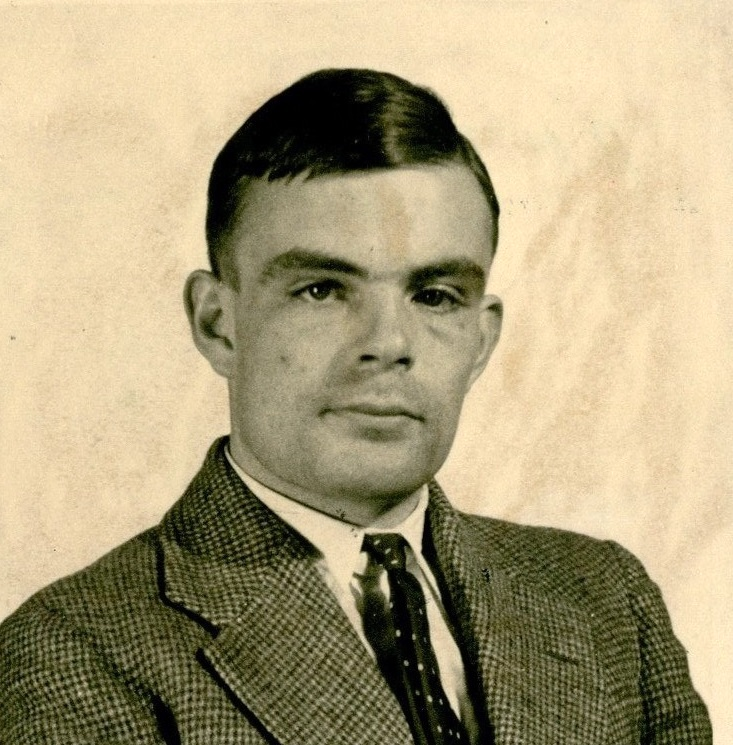
\includegraphics[width=4cm]{data/turing.jpeg}
			};
		\end{tikzpicture}
	\end{frame}

	\setbeamertemplate{footline}[turing]

	\begin{frame}{Historien bak kunstig intelligens} % Turing test
		\begin{tikzpicture}
			\node[] at (0, 0) {};
			\node[] at (10.5, -7.5) {};

			\draw[very thick, gray] (0.5, -1)  -- (1.65, -1) {};

			\node[
				circle,
				draw=activehistory,
				fill=activehistory
			] at (1.65, -1) {};
			\node[
				anchor=north,
				activehistory,
				align=center,
				font=\small\linespread{0.9}\selectfont,
				text height=9pt,
				text depth=3pt,
				inner sep=0pt,
				align=center
			] at (1.65, -1.588) {Turing-\\testen\\(1950)};

			\node[inner sep=0pt, draw=black] (patient) at (5.25, -4.25) {
				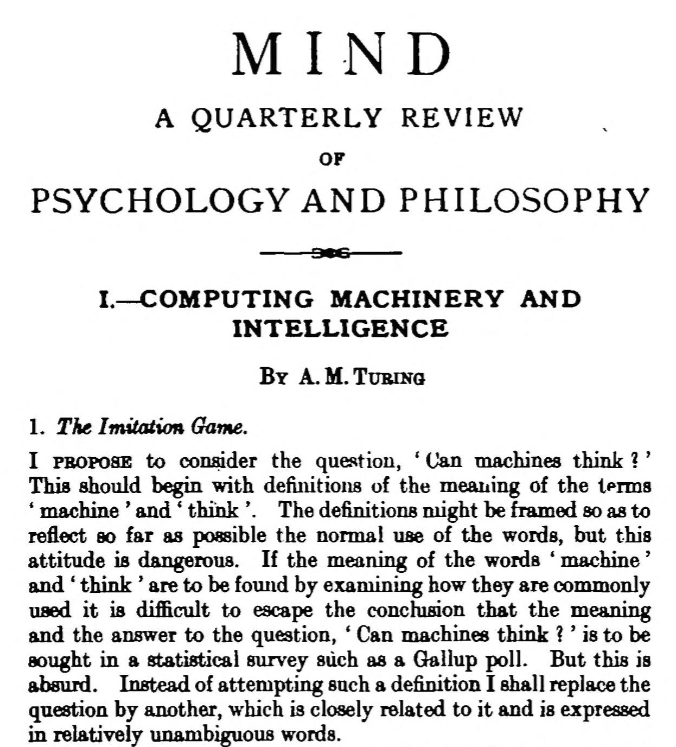
\includegraphics[width=5cm]{data/thinking.png}
			};
		\end{tikzpicture}
	\end{frame}

	\begin{frame}{Historien bak kunstig intelligens} % Dartmouth
		\begin{tikzpicture}
			\node[] at (0, 0) {};
			\node[] at (10.5, -7.5) {};

			\draw[very thick, gray] (0.5, -1)  -- (2.35, -1) {};

			\node[
				circle,
				draw=passivehistory,
				fill=passivehistory
			] at (1.65, -1) {};
			\node[
				anchor=north,
				passivehistory,
				align=center,
				font=\small\linespread{0.9}\selectfont,
				text height=9pt,
				text depth=3pt,
				inner sep=0pt,
				align=center
			] at (1.65, -1.588) {Turing-\\testen\\(1950)};

			\node[
				circle,
				draw=activehistory,
				fill=activehistory,
			] at (2.35, -1) {};
			\node[
				anchor=south,
				activehistory,
				font=\small\linespread{0.9}\selectfont,
				text height=9pt,
				text depth=3pt,
				inner sep=0pt,
				align=center
			] at (2.35, -0.87) {Dartmouth\\(1956)};

			\node[inner sep=0pt] (patient) at (5.25, -4.75) {
				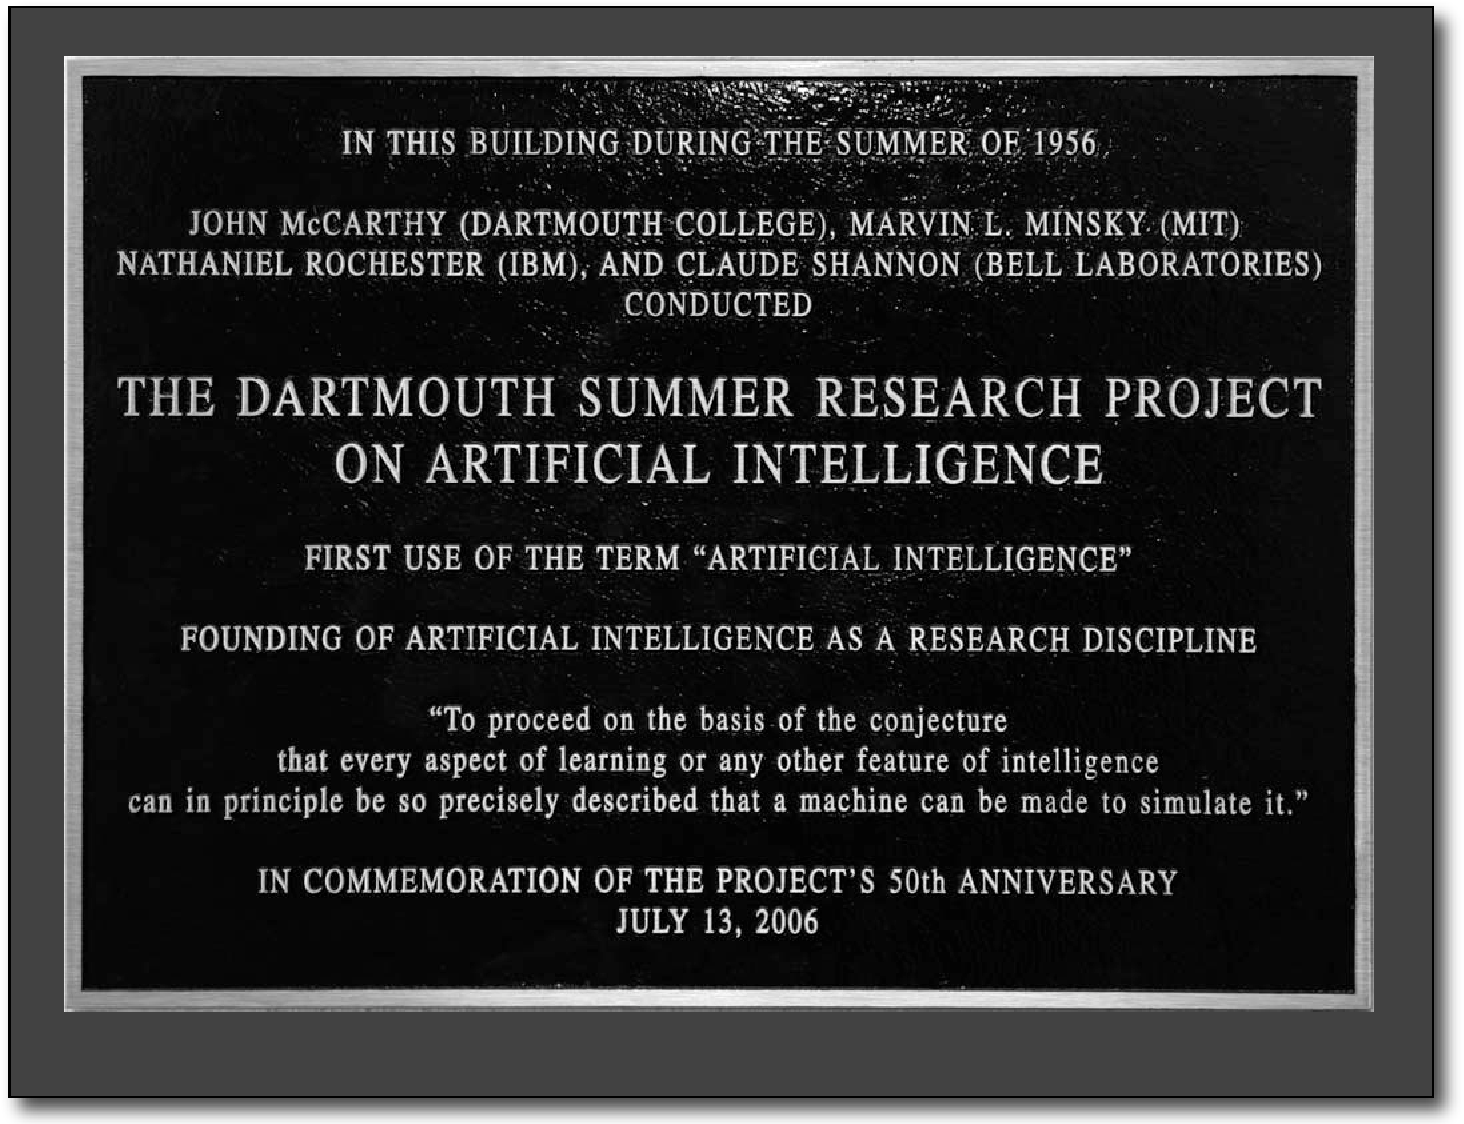
\includegraphics[width=6cm]{data/dartmouth.png}
			};
		\end{tikzpicture}
	\end{frame}

	\setbeamertemplate{footline}[neuron]

	\begin{frame}{Historien bak kunstig intelligens} % Perceptron: Neuron
		\begin{tikzpicture}
			\node[] at (0, 0) {};
			\node[] at (10.5, -7.5) {};

			\draw[very thick, gray] (0.5, -1)  -- (2.68, -1) {};

			\node[
				circle,
				draw=passivehistory,
				fill=passivehistory
			] at (1.65, -1) {};
			\node[
				anchor=north,
				passivehistory,
				align=center,
				font=\small\linespread{0.9}\selectfont,
				text height=9pt,
				text depth=3pt,
				inner sep=0pt,
				align=center
			] at (1.65, -1.588) {Turing-\\testen\\(1950)};

			\node[
				circle,
				draw=passivehistory,
				fill=passivehistory,
			] at (2.35, -1) {};
			\node[
				anchor=south,
				passivehistory,
				font=\small\linespread{0.9}\selectfont,
				text height=9pt,
				text depth=3pt,
				inner sep=0pt,
				align=center
			] at (2.35, -0.87) {Dartmouth\\(1956)};

			\node[
				circle,
				draw=activehistory,
				fill=activehistory,
			] at (2.68, -1) {};
			\node[
				anchor=north,
				activehistory,
				font=\small\linespread{0.9}\selectfont,
				text height=9pt,
				text depth=3pt,
				inner sep=0pt,
				align=center
			] at (2.68, -1.375) {Perceptron\\(1958)};

			\node[draw=black, inner sep=5pt, fill=white] (patient) at (2.875, -4.75) {
				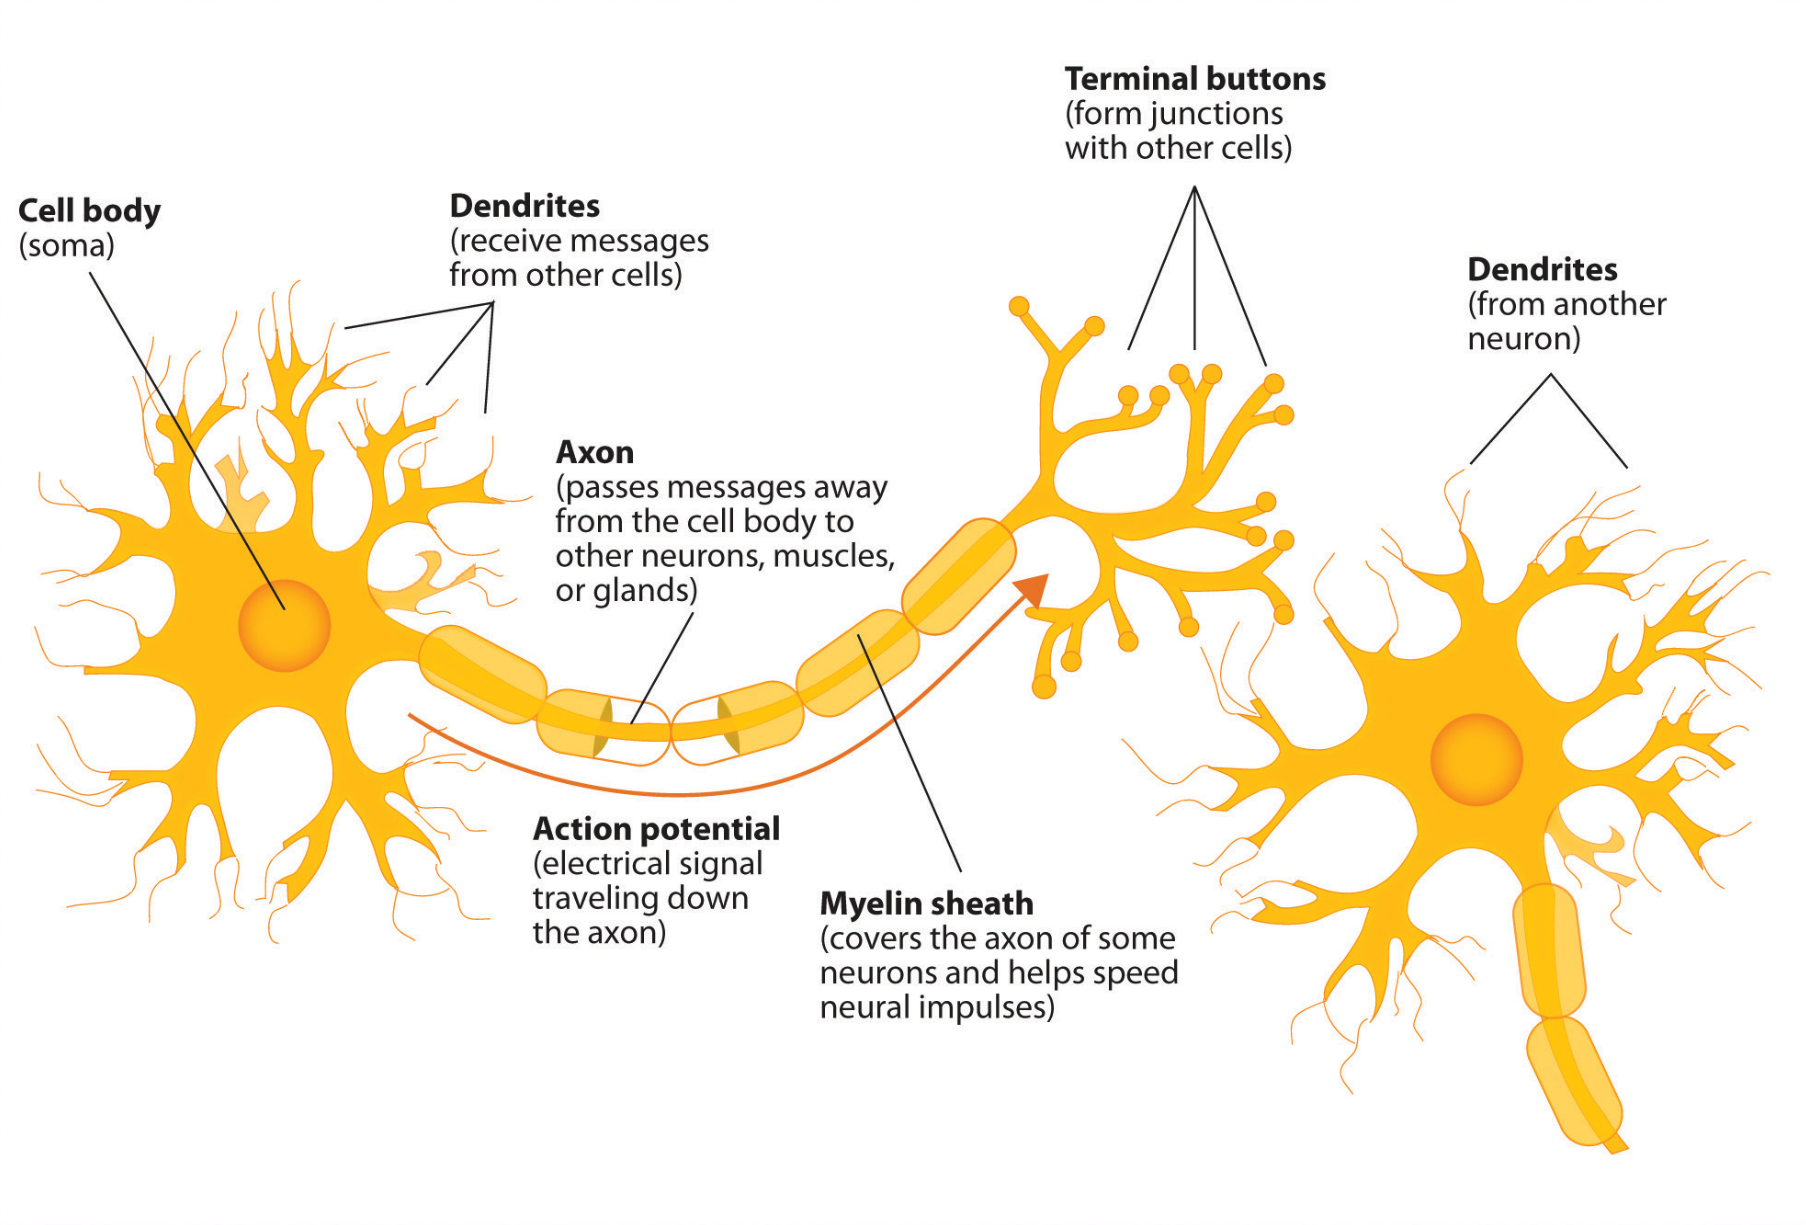
\includegraphics[width=4cm]{data/neuron.png}
			};
		\end{tikzpicture}
	\end{frame}

	\begin{frame}{Historien bak kunstig intelligens} % Perceptron
		\begin{tikzpicture}
			\node[] at (0, 0) {};
			\node[] at (10.5, -7.5) {};

			\draw[very thick, gray] (0.5, -1)  -- (2.68, -1) {};

			\node[
				circle,
				draw=passivehistory,
				fill=passivehistory
			] at (1.65, -1) {};
			\node[
				anchor=north,
				passivehistory,
				align=center,
				font=\small\linespread{0.9}\selectfont,
				text height=9pt,
				text depth=3pt,
				inner sep=0pt,
				align=center
			] at (1.65, -1.588) {Turing-\\testen\\(1950)};

			\node[
				circle,
				draw=passivehistory,
				fill=passivehistory,
			] at (2.35, -1) {};
			\node[
				anchor=south,
				passivehistory,
				font=\small\linespread{0.9}\selectfont,
				text height=9pt,
				text depth=3pt,
				inner sep=0pt,
				align=center
			] at (2.35, -0.87) {Dartmouth\\(1956)};

			\node[
				circle,
				draw=activehistory,
				fill=activehistory,
			] at (2.68, -1) {};
			\node[
				anchor=north,
				activehistory,
				font=\small\linespread{0.9}\selectfont,
				text height=9pt,
				text depth=3pt,
				inner sep=0pt,
				align=center
			] at (2.68, -1.375) {Perceptron\\(1958)};

			\node[draw=black, inner sep=5pt, fill=white] (patient) at (2.875, -4.75) {
				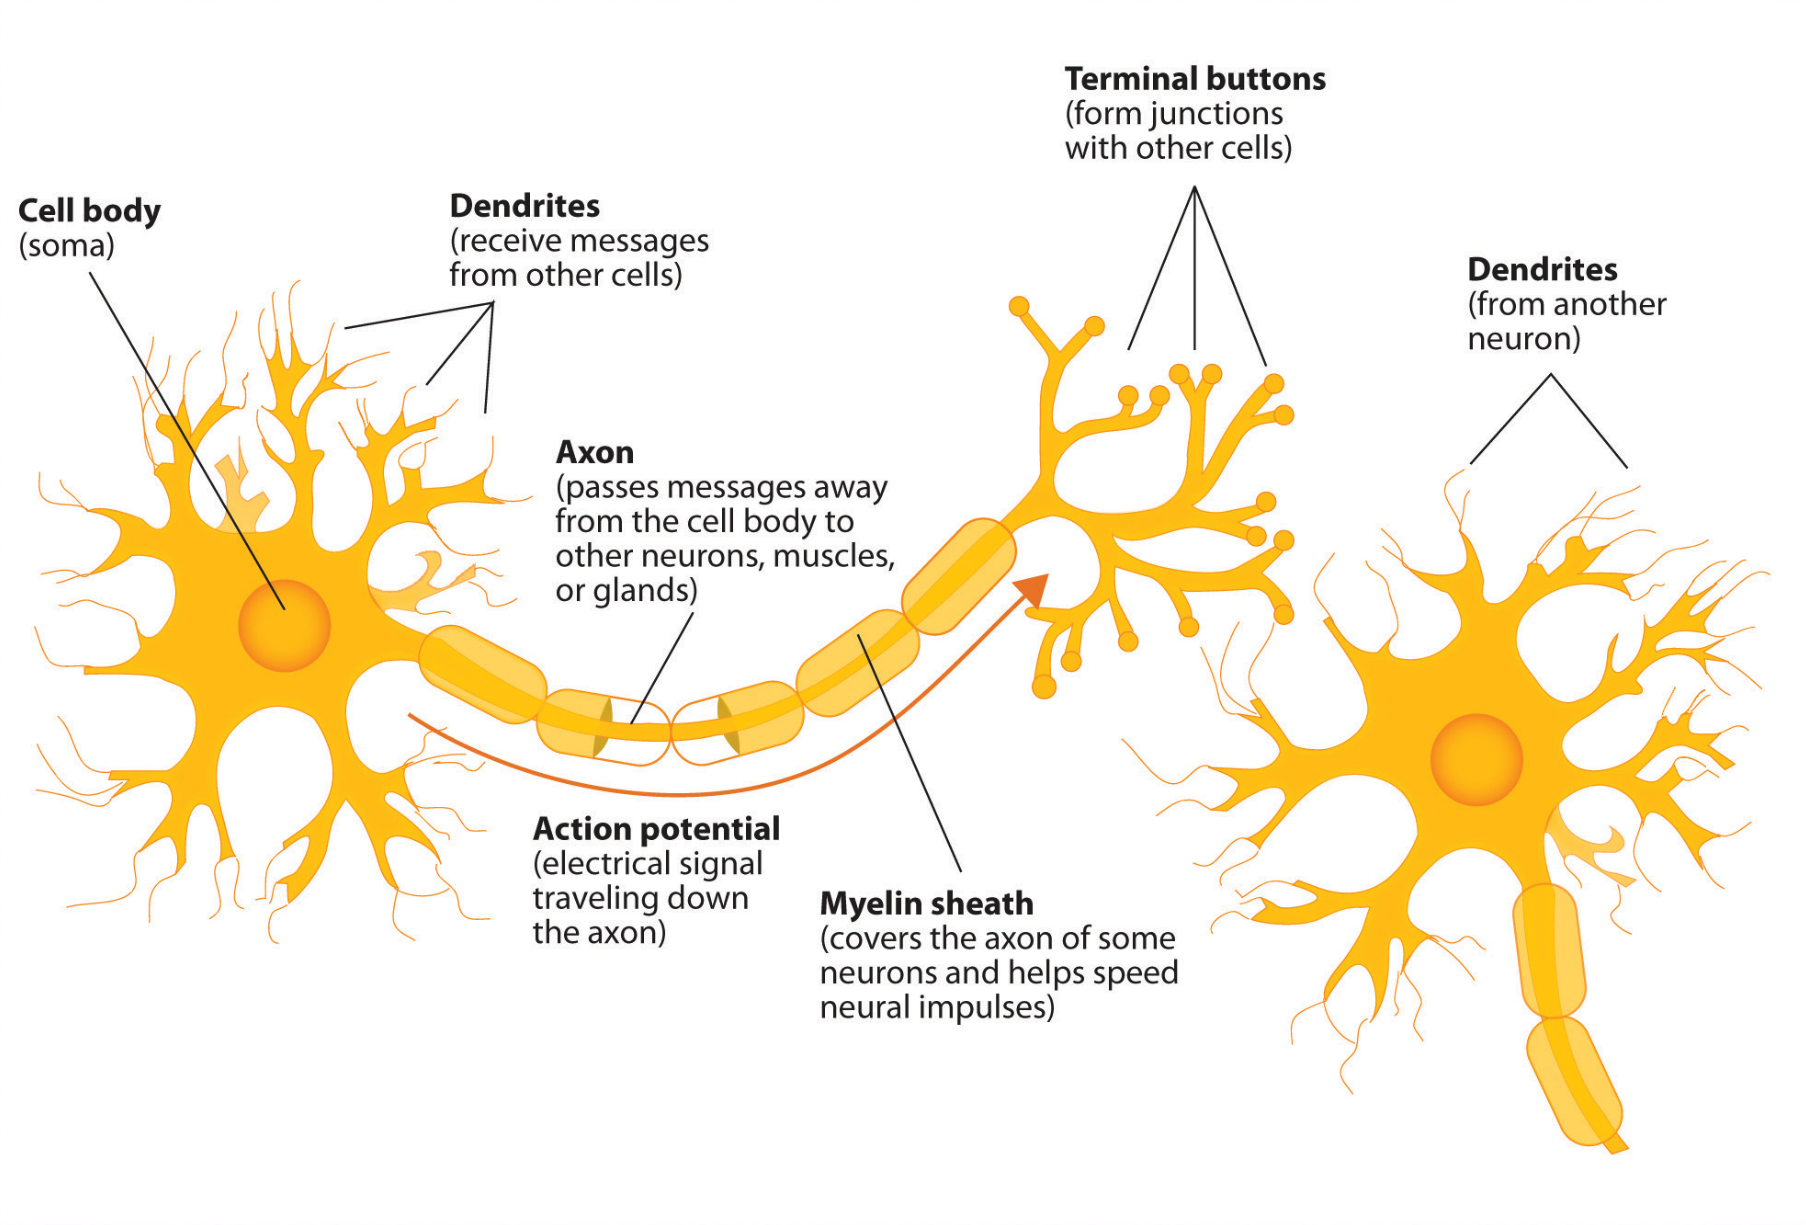
\includegraphics[width=4cm]{data/neuron.png}
			};

			\node[circle, draw=black, fill=nodefill, inner sep=2pt, text depth=0] (node) at (7.625, -4.75) {+};

			\node[] (x0) at (6.375, -3.75) {$\mathrm{input}_0$};
			\node[] (x1) at (6.375, -4.75) {$\mathrm{input}_1$};
			\node[] (x2) at (6.375, -5.75) {$\mathrm{input}_2$};

			\node[align=center] (out) at (8.875, -4.75) {$\mathrm{output}$\\$\mathrm{(0/1)}$};

			\draw[-Latex] (x0) -- (node) node [midway, above] {\small{$w_0$}};
			\draw[-Latex] (x1) -- (node) node [midway, below] {\small{$w_1$}};;
			\draw[-Latex] (x2) -- (node) node [midway, below] {\small{$w_2$}};;
			\draw[-Latex] (node) -- (out);
		\end{tikzpicture}
	\end{frame}

	\setbeamertemplate{footline}[eliza]

	\begin{frame}{Historien bak kunstig intelligens} % Eliza
		\begin{tikzpicture}
			\node[] at (0, 0) {};
			\node[] at (10.5, -7.5) {};

			\draw[very thick, gray] (0.5, -1)  -- (3.28, -1) {};

			\node[
				circle,
				draw=passivehistory,
				fill=passivehistory
			] at (1.65, -1) {};
			\node[
				anchor=north,
				passivehistory,
				align=center,
				font=\small\linespread{0.9}\selectfont,
				text height=9pt,
				text depth=3pt,
				inner sep=0pt,
				align=center
			] at (1.65, -1.588) {Turing-\\testen\\(1950)};

			\node[
				circle,
				draw=passivehistory,
				fill=passivehistory,
			] at (2.35, -1) {};
			\node[
				anchor=south,
				passivehistory,
				font=\small\linespread{0.9}\selectfont,
				text height=9pt,
				text depth=3pt,
				inner sep=0pt,
				align=center
			] at (2.35, -0.87) {Dartmouth\\(1956)};

			\node[
				circle,
				draw=passivehistory,
				fill=passivehistory,
			] at (2.68, -1) {};
			\node[
				anchor=north,
				passivehistory,
				font=\small\linespread{0.9}\selectfont,
				text height=9pt,
				text depth=3pt,
				inner sep=0pt,
				align=center
			] at (2.68, -1.375) {Perceptron\\(1958)};

			\node[
				circle,
				draw=activehistory,
				fill=activehistory
			] at (3.28, -1) {};
			\node[
				anchor=south,
				activehistory,
				font=\small\linespread{0.9}\selectfont,
				text height=9pt,
				text depth=3pt,
				inner sep=0pt,
				align=center
			] at (3.28, -0.87) {Eliza\\(1964)};

			\node[draw=black, inner sep=5pt, fill=white] (patient) at (5.25, -4.75) {
				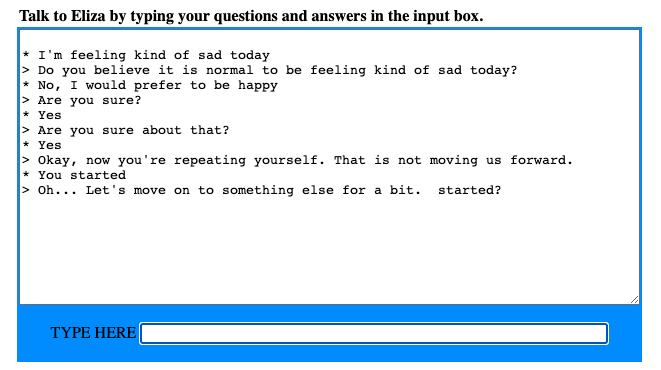
\includegraphics[width=7cm]{data/eliza.png}
			};
		\end{tikzpicture}
	\end{frame}

	\setbeamertemplate{footline}[mycin]

	\begin{frame}{Historien bak kunstig intelligens} % Expert systems: Overview
		\begin{tikzpicture}
			\node[] at (0, 0) {};
			\node[] at (10.5, -7.5) {};

			\draw[very thick, gray] (0.5, -1)  -- (5.13, -1) {};

			\node[
				circle,
				draw=passivehistory,
				fill=passivehistory
			] at (1.65, -1) {};
			\node[
				anchor=north,
				passivehistory,
				align=center,
				font=\small\linespread{0.9}\selectfont,
				text height=9pt,
				text depth=3pt,
				inner sep=0pt,
				align=center
			] at (1.65, -1.588) {Turing-\\testen\\(1950)};

			\node[
				circle,
				draw=passivehistory,
				fill=passivehistory,
			] at (2.35, -1) {};
			\node[
				anchor=south,
				passivehistory,
				font=\small\linespread{0.9}\selectfont,
				text height=9pt,
				text depth=3pt,
				inner sep=0pt,
				align=center
			] at (2.35, -0.87) {Dartmouth\\(1956)};

			\node[
				circle,
				draw=passivehistory,
				fill=passivehistory,
			] at (2.68, -1) {};
			\node[
				anchor=north,
				passivehistory,
				font=\small\linespread{0.9}\selectfont,
				text height=9pt,
				text depth=3pt,
				inner sep=0pt,
				align=center
			] at (2.68, -1.375) {Perceptron\\(1958)};

			\node[
				circle,
				draw=passivehistory,
				fill=passivehistory
			] at (3.28, -1) {};
			\node[
				circle,
				draw=passivehistory,
				fill=passivehistory,
			] at (2.35, -1) {};
			\node[
				anchor=south,
				passivehistory,
				font=\small\linespread{0.9}\selectfont,
				text height=9pt,
				text depth=3pt,
				inner sep=0pt,
				align=center
			] at (3.28, -0.87) {Eliza\\(1964)};

			\node[
				circle,
				draw=activehistory,
				fill=activehistory
			] at (5.13, -1) {};
			\node[
				anchor=north,
				activehistory,
				font=\small\linespread{0.9}\selectfont,
				text height=9pt,
				text depth=3pt,
				inner sep=0pt,
				align=center
			] at (5.13, -1.625) {Ekspert-\\systemer\\(1980)};

			\node[] (patient) at (5.25, -3.25) {
				\Huge{\emoji{face-with-medical-mask}}
			};
			\node[draw=black, align=center ] (interface) at ($ (patient.south) - (0, 0.8) $) {
				User interface
			};

			\node[draw=black] (inference) at ($ (interface.south) - (0, 0.5) $) {
				Inference engine
			};
			\node[draw=black] (database) at ($ (inference.south) - (0, 0.5) $) {
				Knowledge database
			};
			\node[] (doctor) at ($ (database.south) - (0, 0.9) $) {
				\Huge{\emoji{woman-scientist}}
			};

			\draw[-Latex] ($ (patient.south) - (0.1, 0) $) -- ($ (interface.north) - (0.1, 0) $);
			\draw[Latex-] ($ (patient.south) + (0.1, 0) $) -- ($ (interface.north) + (0.1, 0) $);
			\draw[-Latex] ($ (interface.south) - (0.1, 0) $) -- ($ (inference.north) - (0.1, 0) $);
			\draw[Latex-] ($ (interface.south) + (0.1, 0) $) -- ($ (inference.north) + (0.1, 0) $);
			\draw[Latex-] (inference.south) -- (database.north);
			\draw[Latex-, dashed] (database.south) -- (doctor.north);

			\draw[densely dotted] ($ (interface.north west) + (-1.3, 0.1) $) rectangle ($ (database.south east) + (1, -0.1) $);
			\node[anchor=south west] at ($ (interface.north west) + (-1.3, 0.1) $) {MYCIN};

			\node[anchor=north east] at ($ (patient.south) - (0.1, 0.05) $) {\small{Query}};
			\node[anchor=north west] at ($ (patient.south) - (-0.1, 0.05) $) {\small{Response}};
		\end{tikzpicture}
	\end{frame}

	\begin{frame}{Historien bak kunstig intelligens} % Expert systems: Overview
		\begin{tikzpicture}
			\node[] at (0, 0) {};
			\node[] at (10.5, -7.5) {};

			\draw[very thick, gray] (0.5, -1)  -- (5.13, -1) {};

			\node[
				circle,
				draw=passivehistory,
				fill=passivehistory
			] at (1.65, -1) {};
			\node[
				anchor=north,
				passivehistory,
				align=center,
				font=\small\linespread{0.9}\selectfont,
				text height=9pt,
				text depth=3pt,
				inner sep=0pt,
				align=center
			] at (1.65, -1.588) {Turing-\\testen\\(1950)};

			\node[
				circle,
				draw=passivehistory,
				fill=passivehistory,
			] at (2.35, -1) {};
			\node[
				anchor=south,
				passivehistory,
				font=\small\linespread{0.9}\selectfont,
				text height=9pt,
				text depth=3pt,
				inner sep=0pt,
				align=center
			] at (2.35, -0.87) {Dartmouth\\(1956)};

			\node[
				circle,
				draw=passivehistory,
				fill=passivehistory,
			] at (2.68, -1) {};
			\node[
				anchor=north,
				passivehistory,
				font=\small\linespread{0.9}\selectfont,
				text height=9pt,
				text depth=3pt,
				inner sep=0pt,
				align=center
			] at (2.68, -1.375) {Perceptron\\(1958)};

			\node[
				circle,
				draw=passivehistory,
				fill=passivehistory
			] at (3.28, -1) {};
			\node[
				circle,
				draw=passivehistory,
				fill=passivehistory,
			] at (2.35, -1) {};
			\node[
				anchor=south,
				passivehistory,
				font=\small\linespread{0.9}\selectfont,
				text height=9pt,
				text depth=3pt,
				inner sep=0pt,
				align=center
			] at (3.28, -0.87) {Eliza\\(1964)};

			\node[
				circle,
				draw=activehistory,
				fill=activehistory
			] at (5.13, -1) {};
			\node[
				anchor=north,
				activehistory,
				font=\small\linespread{0.9}\selectfont,
				text height=9pt,
				text depth=3pt,
				inner sep=0pt,
				align=center
			] at (5.13, -1.625) {Ekspert-\\systemer\\(1980s)};

			\node[inner sep=0pt, draw=black] (patient) at (5.25, -4.75) {
				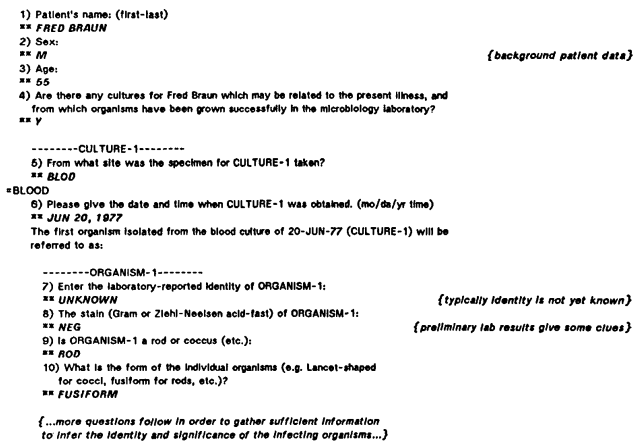
\includegraphics[width=7cm]{data/mycin.png}
			};
		\end{tikzpicture}
	\end{frame}

	\setbeamertemplate{footline}[backprop]

	\begin{frame}{Historien bak kunstig intelligens} % ANN: Perceptron
		\begin{tikzpicture}
			\node[] at (0, 0) {};
			\node[] at (10.5, -7.5) {};

			\draw[very thick, gray] (0.5, -1)  -- (5.82, -1) {};

			\node[
				circle,
				draw=passivehistory,
				fill=passivehistory
			] at (1.65, -1) {};
			\node[
				anchor=north,
				passivehistory,
				align=center,
				font=\small\linespread{0.9}\selectfont,
				text height=9pt,
				text depth=3pt,
				inner sep=0pt,
				align=center
			] at (1.65, -1.588) {Turing-\\testen\\(1950)};

			\node[
				circle,
				draw=passivehistory,
				fill=passivehistory,
			] at (2.35, -1) {};
			\node[
				anchor=south,
				passivehistory,
				font=\small\linespread{0.9}\selectfont,
				text height=9pt,
				text depth=3pt,
				inner sep=0pt,
				align=center
			] at (2.35, -0.87) {Dartmouth\\(1956)};

			\node[
				circle,
				draw=passivehistory,
				fill=passivehistory,
			] at (2.68, -1) {};
			\node[
				anchor=north,
				passivehistory,
				font=\small\linespread{0.9}\selectfont,
				text height=9pt,
				text depth=3pt,
				inner sep=0pt,
				align=center
			] at (2.68, -1.375) {Perceptron\\(1958)};

			\node[
				circle,
				draw=passivehistory,
				fill=passivehistory
			] at (3.28, -1) {};
			\node[
				circle,
				draw=passivehistory,
				fill=passivehistory,
			] at (2.35, -1) {};
			\node[
				anchor=south,
				passivehistory,
				font=\small\linespread{0.9}\selectfont,
				text height=9pt,
				text depth=3pt,
				inner sep=0pt,
				align=center
			] at (3.28, -0.87) {Eliza\\(1964)};

			\node[
				circle,
				draw=passivehistory,
				fill=passivehistory
			] at (5.13, -1) {};
			\node[
				anchor=north,
				passivehistory,
				font=\small\linespread{0.9}\selectfont,
				text height=9pt,
				text depth=3pt,
				inner sep=0pt,
				align=center
			] at (5.13, -1.625) {Ekspert-\\systemer\\(1980s)};

			\node[
				circle,
				draw=activehistory,
				fill=activehistory
			] at (5.82, -1) {};
			\node[
				anchor=south,
				activehistory,
				font=\small\linespread{0.9}\selectfont,
				text height=9pt,
				text depth=3pt,
				inner sep=0pt,
				align=center
			] at (5.82, -0.87) {ANN\\(1986)};

			\node[inner sep=0pt, minimum size=0.4cm, draw=black, circle, fill=nodefill] (n00) at (5.25, -4.75) {};

			\node[] (x0) at (4, -4) {$\mathrm{input}_0$};
			\node[] (x1) at (4, -4.75) {$\mathrm{input}_1$};
			\node[] (x2) at (4, -5.5) {$\mathrm{input}_2$};

			\node[] (out) at (6.5, -4.75) {$\mathrm{output}$};

			\draw[-] (x0.east) -- (n00);
			\draw[-] (x1.east) -- (n00);
			\draw[-] (x2.east) -- (n00);

			\draw[->] (n00) -- (out);
		\end{tikzpicture}
	\end{frame}

	\begin{frame}{Historien bak kunstig intelligens} % ANN: Neural net
		\begin{tikzpicture}
			\node[] at (0, 0) {};
			\node[] at (10.5, -7.5) {};

			\draw[very thick, gray] (0.5, -1)  -- (5.82, -1) {};

			\node[
				circle,
				draw=passivehistory,
				fill=passivehistory
			] at (1.65, -1) {};
			\node[
				anchor=north,
				passivehistory,
				align=center,
				font=\small\linespread{0.9}\selectfont,
				text height=9pt,
				text depth=3pt,
				inner sep=0pt,
				align=center
			] at (1.65, -1.588) {Turing-\\testen\\(1950)};

			\node[
				circle,
				draw=passivehistory,
				fill=passivehistory,
			] at (2.35, -1) {};
			\node[
				anchor=south,
				passivehistory,
				font=\small\linespread{0.9}\selectfont,
				text height=9pt,
				text depth=3pt,
				inner sep=0pt,
				align=center
			] at (2.35, -0.87) {Dartmouth\\(1956)};

			\node[
				circle,
				draw=passivehistory,
				fill=passivehistory,
			] at (2.68, -1) {};
			\node[
				anchor=north,
				passivehistory,
				font=\small\linespread{0.9}\selectfont,
				text height=9pt,
				text depth=3pt,
				inner sep=0pt,
				align=center
			] at (2.68, -1.375) {Perceptron\\(1958)};

			\node[
				circle,
				draw=passivehistory,
				fill=passivehistory
			] at (3.28, -1) {};
			\node[
				circle,
				draw=passivehistory,
				fill=passivehistory,
			] at (2.35, -1) {};
			\node[
				anchor=south,
				passivehistory,
				font=\small\linespread{0.9}\selectfont,
				text height=9pt,
				text depth=3pt,
				inner sep=0pt,
				align=center
			] at (3.28, -0.87) {Eliza\\(1964)};

			\node[
				circle,
				draw=passivehistory,
				fill=passivehistory
			] at (5.13, -1) {};
			\node[
				anchor=north,
				passivehistory,
				font=\small\linespread{0.9}\selectfont,
				text height=9pt,
				text depth=3pt,
				inner sep=0pt,
				align=center
			] at (5.13, -1.625) {Ekspert-\\systemer\\(1980s)};

			\node[
				circle,
				draw=activehistory,
				fill=activehistory
			] at (5.82, -1) {};
			\node[
				anchor=south,
				activehistory,
				font=\small\linespread{0.9}\selectfont,
				text height=9pt,
				text depth=3pt,
				inner sep=0pt,
				align=center
			] at (5.82, -0.87) {ANN\\(1986)};

			\node[] (x0) at (2.5, -4) {$\mathrm{input}_0$};
			\node[] (x1) at (2.5, -4.75) {$\mathrm{input}_1$};
			\node[] (x2) at (2.5, -5.5) {$\mathrm{input}_2$};

			\node[inner sep=0pt, minimum size=0.4cm, draw=black, circle, fill=nodefill] (n00) at (3.75, -3.75) {};
			\node[inner sep=0pt, minimum size=0.4cm, draw=black, circle, fill=nodefill] (n01) at (3.75, -4.25) {};
			\node[inner sep=0pt, minimum size=0.4cm, draw=black, circle, fill=nodefill] (n02) at (3.75, -4.75) {};
			\node[inner sep=0pt, minimum size=0.4cm, draw=black, circle, fill=nodefill] (n03) at (3.75, -5.25) {};
			\node[inner sep=0pt, minimum size=0.4cm, draw=black, circle, fill=nodefill] (n04) at (3.75, -5.75) {};

			\node[inner sep=0pt, minimum size=0.4cm, draw=black, circle, fill=nodefill] (n10) at (4.5, -4) {};
			\node[inner sep=0pt, minimum size=0.4cm, draw=black, circle, fill=nodefill] (n11) at (4.5, -4.5) {};
			\node[inner sep=0pt, minimum size=0.4cm, draw=black, circle, fill=nodefill] (n12) at (4.5, -5) {};
			\node[inner sep=0pt, minimum size=0.4cm, draw=black, circle, fill=nodefill] (n13) at (4.5, -5.5) {};

			\node[inner sep=0pt, minimum size=0.4cm, draw=black, circle, fill=nodefill] (n20) at (5.25, -4.25) {};
			\node[inner sep=0pt, minimum size=0.4cm, draw=black, circle, fill=nodefill] (n21) at (5.25, -4.75) {};
			\node[inner sep=0pt, minimum size=0.4cm, draw=black, circle, fill=nodefill] (n22) at (5.25, -5.25) {};

			\node[inner sep=0pt, minimum size=0.4cm, draw=black, circle, fill=nodefill] (n30) at (6, -4.5) {};
			\node[inner sep=0pt, minimum size=0.4cm, draw=black, circle, fill=nodefill] (n31) at (6, -5) {};

			\node[inner sep=0pt, minimum size=0.4cm, draw=black, circle, fill=nodefill, text depth=0] (n40) at (6.75, -4.75) {};
			\node[] (out) at (8, -4.75) {$\mathrm{output}$};

			\draw[-] (x0.east) -- (n00);
			\draw[-] (x0.east) -- (n01);
			\draw[-] (x0.east) -- (n02);
			\draw[-] (x0.east) -- (n03);
			\draw[-] (x0.east) -- (n04);
			\draw[-] (x1.east) -- (n00);
			\draw[-] (x1.east) -- (n01);
			\draw[-] (x1.east) -- (n02);
			\draw[-] (x1.east) -- (n03);
			\draw[-] (x1.east) -- (n04);
			\draw[-] (x2.east) -- (n00);
			\draw[-] (x2.east) -- (n01);
			\draw[-] (x2.east) -- (n02);
			\draw[-] (x2.east) -- (n03);
			\draw[-] (x2.east) -- (n04);

			\draw[-] (n00) -- (n10);
			\draw[-] (n00) -- (n11);
			\draw[-] (n00) -- (n12);
			\draw[-] (n00) -- (n13);
			\draw[-] (n01) -- (n10);
			\draw[-] (n01) -- (n11);
			\draw[-] (n01) -- (n12);
			\draw[-] (n01) -- (n13);
			\draw[-] (n02) -- (n10);
			\draw[-] (n02) -- (n11);
			\draw[-] (n02) -- (n12);
			\draw[-] (n02) -- (n13);
			\draw[-] (n03) -- (n10);
			\draw[-] (n03) -- (n11);
			\draw[-] (n03) -- (n12);
			\draw[-] (n03) -- (n13);
			\draw[-] (n04) -- (n10);
			\draw[-] (n04) -- (n11);
			\draw[-] (n04) -- (n12);
			\draw[-] (n04) -- (n13);

			\draw[-] (n10) -- (n20);
			\draw[-] (n10) -- (n21);
			\draw[-] (n10) -- (n22);
			\draw[-] (n11) -- (n20);
			\draw[-] (n11) -- (n21);
			\draw[-] (n11) -- (n22);
			\draw[-] (n12) -- (n20);
			\draw[-] (n12) -- (n21);
			\draw[-] (n12) -- (n22);
			\draw[-] (n13) -- (n20);
			\draw[-] (n13) -- (n21);
			\draw[-] (n13) -- (n22);

			\draw[-] (n20) -- (n30);
			\draw[-] (n20) -- (n31);
			\draw[-] (n21) -- (n30);
			\draw[-] (n21) -- (n31);
			\draw[-] (n22) -- (n30);
			\draw[-] (n22) -- (n31);

			\draw[-] (n30) -- (n40);
			\draw[-] (n31) -- (n40);

			\draw[->] (n40) -- (out);
		\end{tikzpicture}
	\end{frame}

	\begin{frame}{Historien bak kunstig intelligens} % ANN: Paper
		\begin{tikzpicture}
			\node[] at (0, 0) {};
			\node[] at (10.5, -7.5) {};

			\draw[very thick, gray] (0.5, -1)  -- (5.82, -1) {};

			\node[
				circle,
				draw=passivehistory,
				fill=passivehistory
			] at (1.65, -1) {};
			\node[
				anchor=north,
				passivehistory,
				align=center,
				font=\small\linespread{0.9}\selectfont,
				text height=9pt,
				text depth=3pt,
				inner sep=0pt,
				align=center
			] at (1.65, -1.588) {Turing-\\testen\\(1950)};

			\node[
				circle,
				draw=passivehistory,
				fill=passivehistory,
			] at (2.35, -1) {};
			\node[
				anchor=south,
				passivehistory,
				font=\small\linespread{0.9}\selectfont,
				text height=9pt,
				text depth=3pt,
				inner sep=0pt,
				align=center
			] at (2.35, -0.87) {Dartmouth\\(1956)};

			\node[
				circle,
				draw=passivehistory,
				fill=passivehistory,
			] at (2.68, -1) {};
			\node[
				anchor=north,
				passivehistory,
				font=\small\linespread{0.9}\selectfont,
				text height=9pt,
				text depth=3pt,
				inner sep=0pt,
				align=center
			] at (2.68, -1.375) {Perceptron\\(1958)};

			\node[
				circle,
				draw=passivehistory,
				fill=passivehistory
			] at (3.28, -1) {};
			\node[
				circle,
				draw=passivehistory,
				fill=passivehistory,
			] at (2.35, -1) {};
			\node[
				anchor=south,
				passivehistory,
				font=\small\linespread{0.9}\selectfont,
				text height=9pt,
				text depth=3pt,
				inner sep=0pt,
				align=center
			] at (3.28, -0.87) {Eliza\\(1964)};

			\node[
				circle,
				draw=passivehistory,
				fill=passivehistory
			] at (5.13, -1) {};
			\node[
				anchor=north,
				passivehistory,
				font=\small\linespread{0.9}\selectfont,
				text height=9pt,
				text depth=3pt,
				inner sep=0pt,
				align=center
			] at (5.13, -1.625) {Ekspert-\\systemer\\(1980s)};

			\node[
				circle,
				draw=activehistory,
				fill=activehistory
			] at (5.82, -1) {};
			\node[
				anchor=south,
				activehistory,
				font=\small\linespread{0.9}\selectfont,
				text height=9pt,
				text depth=3pt,
				inner sep=0pt,
				align=center
			] at (5.82, -0.87) {ANN\\(1986)};

			\node[inner sep=0pt, draw=black] (img3) at (5.25, -4.75) {
				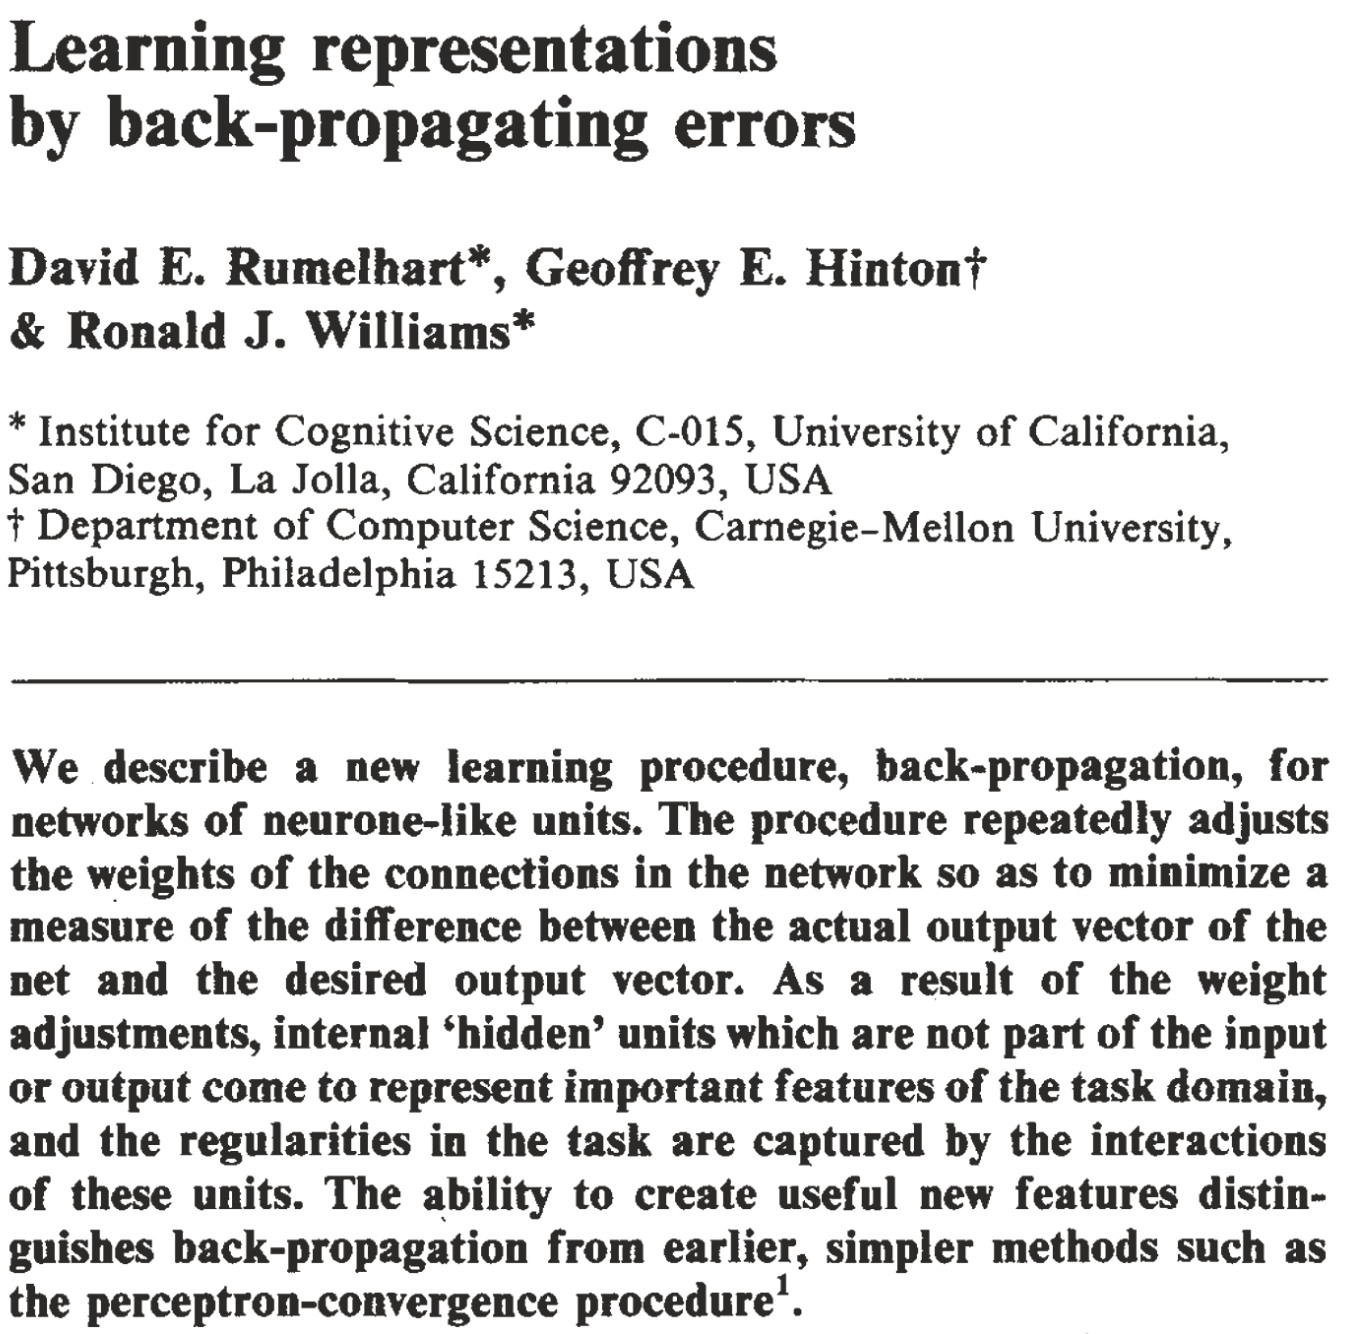
\includegraphics[width=4cm]{data/backprop.png}
			};
		\end{tikzpicture}
	\end{frame}

	\begin{frame}{Historien bak kunstig intelligens} % ANN: Backprop
		\begin{tikzpicture}
			\node[] at (0, 0) {};
			\node[] at (10.5, -7.5) {};

			\draw[very thick, gray] (0.5, -1)  -- (5.82, -1) {};

			\node[
				circle,
				draw=passivehistory,
				fill=passivehistory
			] at (1.65, -1) {};
			\node[
				anchor=north,
				passivehistory,
				align=center,
				font=\small\linespread{0.9}\selectfont,
				text height=9pt,
				text depth=3pt,
				inner sep=0pt,
				align=center
			] at (1.65, -1.588) {Turing-\\testen\\(1950)};

			\node[
				circle,
				draw=passivehistory,
				fill=passivehistory,
			] at (2.35, -1) {};
			\node[
				anchor=south,
				passivehistory,
				font=\small\linespread{0.9}\selectfont,
				text height=9pt,
				text depth=3pt,
				inner sep=0pt,
				align=center
			] at (2.35, -0.87) {Dartmouth\\(1956)};

			\node[
				circle,
				draw=passivehistory,
				fill=passivehistory,
			] at (2.68, -1) {};
			\node[
				anchor=north,
				passivehistory,
				font=\small\linespread{0.9}\selectfont,
				text height=9pt,
				text depth=3pt,
				inner sep=0pt,
				align=center
			] at (2.68, -1.375) {Perceptron\\(1958)};

			\node[
				circle,
				draw=passivehistory,
				fill=passivehistory
			] at (3.28, -1) {};
			\node[
				circle,
				draw=passivehistory,
				fill=passivehistory,
			] at (2.35, -1) {};
			\node[
				anchor=south,
				passivehistory,
				font=\small\linespread{0.9}\selectfont,
				text height=9pt,
				text depth=3pt,
				inner sep=0pt,
				align=center
			] at (3.28, -0.87) {Eliza\\(1964)};

			\node[
				circle,
				draw=passivehistory,
				fill=passivehistory
			] at (5.13, -1) {};
			\node[
				anchor=north,
				passivehistory,
				font=\small\linespread{0.9}\selectfont,
				text height=9pt,
				text depth=3pt,
				inner sep=0pt,
				align=center
			] at (5.13, -1.625) {Ekspert-\\systemer\\(1980s)};

			\node[
				circle,
				draw=activehistory,
				fill=activehistory
			] at (5.82, -1) {};
			\node[
				anchor=south,
				activehistory,
				font=\small\linespread{0.9}\selectfont,
				text height=9pt,
				text depth=3pt,
				inner sep=0pt,
				align=center
			] at (5.82, -0.87) {ANN\\(1986)};

			\node[] (x0) at (2.5, -4) {$\mathrm{input}_0$};
			\node[] (x1) at (2.5, -4.75) {$\mathrm{input}_1$};
			\node[] (x2) at (2.5, -5.5) {$\mathrm{input}_2$};

			\node[inner sep=0pt, minimum size=0.4cm, draw=black, circle, fill=nodefill] (n00) at (3.75, -3.75) {};
			\node[inner sep=0pt, minimum size=0.4cm, draw=black, circle, fill=nodefill] (n01) at (3.75, -4.25) {};
			\node[inner sep=0pt, minimum size=0.4cm, draw=black, circle, fill=nodefill] (n02) at (3.75, -4.75) {};
			\node[inner sep=0pt, minimum size=0.4cm, draw=black, circle, fill=nodefill] (n03) at (3.75, -5.25) {};
			\node[inner sep=0pt, minimum size=0.4cm, draw=black, circle, fill=nodefill] (n04) at (3.75, -5.75) {};

			\node[inner sep=0pt, minimum size=0.4cm, draw=black, circle, fill=nodefill] (n10) at (4.5, -4) {};
			\node[inner sep=0pt, minimum size=0.4cm, draw=black, circle, fill=nodefill] (n11) at (4.5, -4.5) {};
			\node[inner sep=0pt, minimum size=0.4cm, draw=black, circle, fill=nodefill] (n12) at (4.5, -5) {};
			\node[inner sep=0pt, minimum size=0.4cm, draw=black, circle, fill=nodefill] (n13) at (4.5, -5.5) {};

			\node[inner sep=0pt, minimum size=0.4cm, draw=black, circle, fill=nodefill] (n20) at (5.25, -4.25) {};
			\node[inner sep=0pt, minimum size=0.4cm, draw=black, circle, fill=nodefill] (n21) at (5.25, -4.75) {};
			\node[inner sep=0pt, minimum size=0.4cm, draw=black, circle, fill=nodefill] (n22) at (5.25, -5.25) {};

			\node[inner sep=0pt, minimum size=0.4cm, draw=black, circle, fill=nodefill] (n30) at (6, -4.5) {};
			\node[inner sep=0pt, minimum size=0.4cm, draw=black, circle, fill=nodefill] (n31) at (6, -5) {};

			\node[inner sep=0pt, minimum size=0.4cm, draw=black, circle, fill=nodefill, text depth=0] (n40) at (6.75, -4.75) {};
			\node[] (out) at (8, -4.75) {$\mathrm{output}$};

			\draw[-] (x0.east) -- (n00);
			\draw[-] (x0.east) -- (n01);
			\draw[-] (x0.east) -- (n02);
			\draw[-] (x0.east) -- (n03);
			\draw[-] (x0.east) -- (n04);
			\draw[-] (x1.east) -- (n00);
			\draw[-] (x1.east) -- (n01);
			\draw[-] (x1.east) -- (n02);
			\draw[-] (x1.east) -- (n03);
			\draw[-] (x1.east) -- (n04);
			\draw[-] (x2.east) -- (n00);
			\draw[-] (x2.east) -- (n01);
			\draw[-] (x2.east) -- (n02);
			\draw[-] (x2.east) -- (n03);
			\draw[-] (x2.east) -- (n04);

			\draw[Latex-, red] (n00) -- (n10);
			\draw[Latex-, red] (n00) -- (n11);
			\draw[Latex-, red] (n00) -- (n12);
			\draw[Latex-, red] (n00) -- (n13);
			\draw[Latex-, red] (n01) -- (n10);
			\draw[Latex-, red] (n01) -- (n11);
			\draw[Latex-, red] (n01) -- (n12);
			\draw[Latex-, red] (n01) -- (n13);
			\draw[Latex-, red] (n02) -- (n10);
			\draw[Latex-, red] (n02) -- (n11);
			\draw[Latex-, red] (n02) -- (n12);
			\draw[Latex-, red] (n02) -- (n13);
			\draw[Latex-, red] (n03) -- (n10);
			\draw[Latex-, red] (n03) -- (n11);
			\draw[Latex-, red] (n03) -- (n12);
			\draw[Latex-, red] (n03) -- (n13);
			\draw[Latex-, red] (n04) -- (n10);
			\draw[Latex-, red] (n04) -- (n11);
			\draw[Latex-, red] (n04) -- (n12);
			\draw[Latex-, red] (n04) -- (n13);

			\draw[Latex-, red] (n10) -- (n20);
			\draw[Latex-, red] (n10) -- (n21);
			\draw[Latex-, red] (n10) -- (n22);
			\draw[Latex-, red] (n11) -- (n20);
			\draw[Latex-, red] (n11) -- (n21);
			\draw[Latex-, red] (n11) -- (n22);
			\draw[Latex-, red] (n12) -- (n20);
			\draw[Latex-, red] (n12) -- (n21);
			\draw[Latex-, red] (n12) -- (n22);
			\draw[Latex-, red] (n13) -- (n20);
			\draw[Latex-, red] (n13) -- (n21);
			\draw[Latex-, red] (n13) -- (n22);

			\draw[Latex-, red] (n20) -- (n30);
			\draw[Latex-, red] (n20) -- (n31);
			\draw[Latex-, red] (n21) -- (n30);
			\draw[Latex-, red] (n21) -- (n31);
			\draw[Latex-, red] (n22) -- (n30);
			\draw[Latex-, red] (n22) -- (n31);

			\draw[Latex-, red] (n30) -- (n40);
			\draw[Latex-, red] (n31) -- (n40);

			\draw[Latex-, red] (n40) -- (out);
		\end{tikzpicture}
	\end{frame}

	\setbeamertemplate{footline}[default]

	\begin{frame}{Historien bak kunstig intelligens} % Deep blue
		\begin{tikzpicture}
			\node[] at (0, 0) {};
			\node[] at (10.5, -7.5) {};

			\draw[very thick, gray] (0.5, -1)  -- (7.1, -1) {};

			\node[
				circle,
				draw=passivehistory,
				fill=passivehistory
			] at (1.65, -1) {};
			\node[
				anchor=north,
				passivehistory,
				align=center,
				font=\small\linespread{0.9}\selectfont,
				text height=9pt,
				text depth=3pt,
				inner sep=0pt,
				align=center
			] at (1.65, -1.588) {Turing-\\testen\\(1950)};

			\node[
				circle,
				draw=passivehistory,
				fill=passivehistory,
			] at (2.35, -1) {};
			\node[
				anchor=south,
				passivehistory,
				font=\small\linespread{0.9}\selectfont,
				text height=9pt,
				text depth=3pt,
				inner sep=0pt,
				align=center
			] at (2.35, -0.87) {Dartmouth\\(1956)};

			\node[
				circle,
				draw=passivehistory,
				fill=passivehistory,
			] at (2.68, -1) {};
			\node[
				anchor=north,
				passivehistory,
				font=\small\linespread{0.9}\selectfont,
				text height=9pt,
				text depth=3pt,
				inner sep=0pt,
				align=center
			] at (2.68, -1.375) {Perceptron\\(1958)};

			\node[
				circle,
				draw=passivehistory,
				fill=passivehistory
			] at (3.28, -1) {};
			\node[
				circle,
				draw=passivehistory,
				fill=passivehistory,
			] at (2.35, -1) {};
			\node[
				anchor=south,
				passivehistory,
				font=\small\linespread{0.9}\selectfont,
				text height=9pt,
				text depth=3pt,
				inner sep=0pt,
				align=center
			] at (3.28, -0.87) {Eliza\\(1964)};

			\node[
				circle,
				draw=passivehistory,
				fill=passivehistory
			] at (5.13, -1) {};
			\node[
				anchor=north,
				passivehistory,
				font=\small\linespread{0.9}\selectfont,
				text height=9pt,
				text depth=3pt,
				inner sep=0pt,
				align=center
			] at (5.13, -1.625) {Ekspert-\\systemer\\(1980s)};

			\node[
				circle,
				draw=passivehistory,
				fill=passivehistory
			] at (5.82, -1) {};
			\node[
				anchor=south,
				passivehistory,
				font=\small\linespread{0.9}\selectfont,
				text height=9pt,
				text depth=3pt,
				inner sep=0pt,
				align=center
			] at (5.82, -0.87) {ANN\\(1986)};

			\node[
				circle,
				draw=activehistory,
				fill=activehistory
			] at (7.10, -1) {};
			\node[
				anchor=north,
				activehistory,
				font=\small\linespread{0.9}\selectfont,
				text height=9pt,
				text depth=3pt,
				inner sep=0pt,
				align=center
			] at (7.10, -1.372) {Deep blue\\(1997)};

			\node[inner sep=0pt, draw=black, label=below:{\small{DALL-E: "A robot playing chess"}}] (img) at (2.75, -4.75) {
				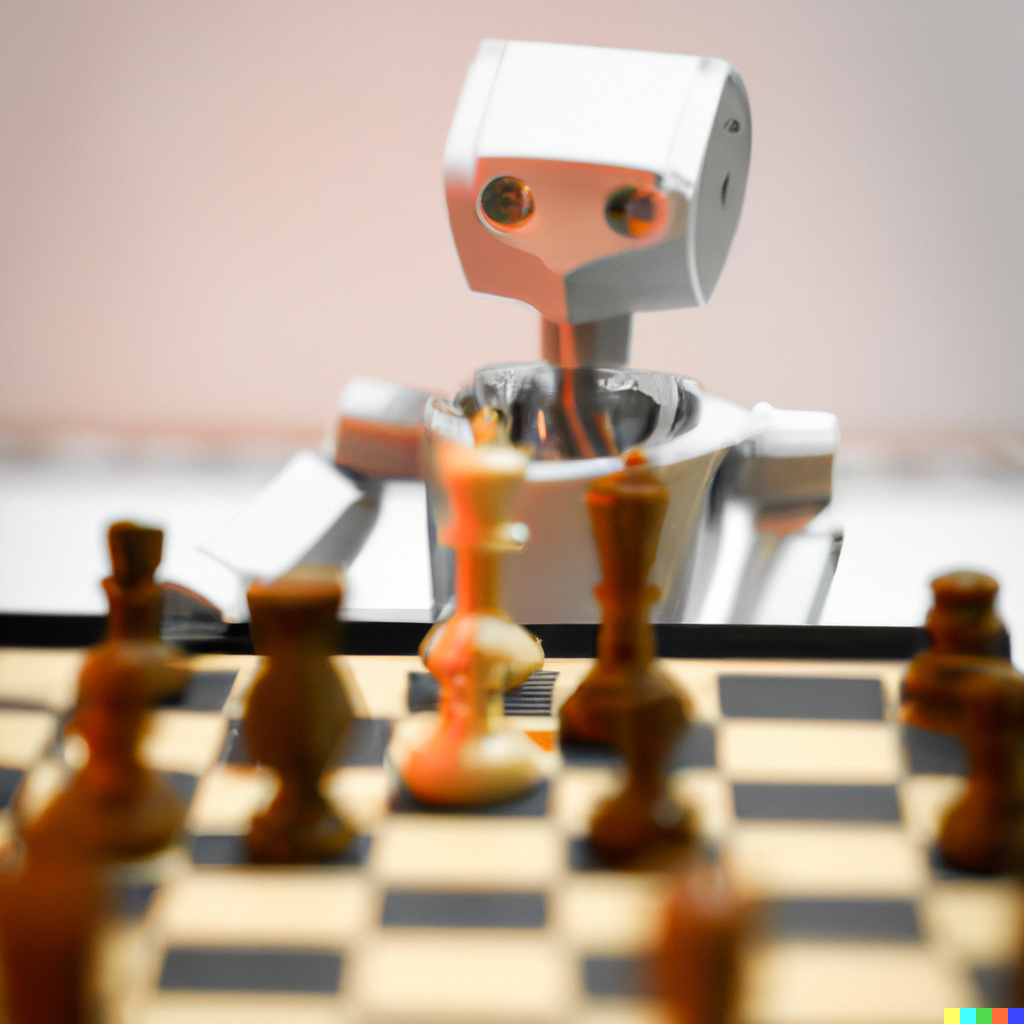
\includegraphics[width=4cm]{data/chess.png}
			};
			\node[anchor=north west, align=left] at ($ (img.north east)  + (0.1, 0) $) {
				\bullet\hspace{0.1cm}IBMs Deep Blue slår Garry Kasparov og\\blir den første datamaskinen til å slå den\\sittende verdensmesteren i sjakk.\\
				\bullet\hspace{0.1cm}Deep blue vant med 3\textonehalf { }poeng mot\\Kasparovs 2\textonehalf{ } over 6 spill.\\
				\bullet\hspace{0.1cm}Kasparov uttalte at \\"Deep Blue was intelligent the way your\\programmable alarm clock is intelligent."\\
				\bullet\hspace{0.1cm}Kombinasjon av maskinlæring og\\hardkodet kunnskap fra sjakkeksperter.
			};
		\end{tikzpicture}
	\end{frame}

	\begin{frame}{Historien bak kunstig intelligens} %DL (image classification)
		\begin{tikzpicture}
			\node[] at (0, 0) {};
			\node[] at (10.5, -7.5) {};

			\draw[very thick, gray] (0.5, -1)  -- (8.84, -1) {};

			\node[
				circle,
				draw=passivehistory,
				fill=passivehistory
			] at (1.65, -1) {};
			\node[
				anchor=north,
				passivehistory,
				align=center,
				font=\small\linespread{0.9}\selectfont,
				text height=9pt,
				text depth=3pt,
				inner sep=0pt,
				align=center
			] at (1.65, -1.588) {Turing-\\testen\\(1950)};

			\node[
				circle,
				draw=passivehistory,
				fill=passivehistory,
			] at (2.35, -1) {};
			\node[
				anchor=south,
				passivehistory,
				font=\small\linespread{0.9}\selectfont,
				text height=9pt,
				text depth=3pt,
				inner sep=0pt,
				align=center
			] at (2.35, -0.87) {Dartmouth\\(1956)};

			\node[
				circle,
				draw=passivehistory,
				fill=passivehistory,
			] at (2.68, -1) {};
			\node[
				anchor=north,
				passivehistory,
				font=\small\linespread{0.9}\selectfont,
				text height=9pt,
				text depth=3pt,
				inner sep=0pt,
				align=center
			] at (2.68, -1.375) {Perceptron\\(1958)};

			\node[
				circle,
				draw=passivehistory,
				fill=passivehistory
			] at (3.28, -1) {};
			\node[
				circle,
				draw=passivehistory,
				fill=passivehistory,
			] at (2.35, -1) {};
			\node[
				anchor=south,
				passivehistory,
				font=\small\linespread{0.9}\selectfont,
				text height=9pt,
				text depth=3pt,
				inner sep=0pt,
				align=center
			] at (3.28, -0.87) {Eliza\\(1964)};

			\node[
				circle,
				draw=passivehistory,
				fill=passivehistory
			] at (5.13, -1) {};
			\node[
				anchor=north,
				passivehistory,
				font=\small\linespread{0.9}\selectfont,
				text height=9pt,
				text depth=3pt,
				inner sep=0pt,
				align=center
			] at (5.13, -1.625) {Ekspert-\\systemer\\(1980s)};

			\node[
				circle,
				draw=passivehistory,
				fill=passivehistory
			] at (5.82, -1) {};
			\node[
				anchor=south,
				passivehistory,
				font=\small\linespread{0.9}\selectfont,
				text height=9pt,
				text depth=3pt,
				inner sep=0pt,
				align=center
			] at (5.82, -0.87) {ANN\\(1986)};

			\node[
				circle,
				draw=passivehistory,
				fill=passivehistory
			] at (7.10, -1) {};
			\node[
				anchor=north,
				passivehistory,
				font=\small\linespread{0.9}\selectfont,
				text height=9pt,
				text depth=3pt,
				inner sep=0pt,
				align=center
			] at (7.10, -1.372) {Deep blue\\(1997)};

			\node[
				circle,
				draw=activehistory,
				fill=activehistory
			] at (8.84, -1) {};
			\node[
				anchor=south,
				activehistory,
				font=\small\linespread{0.9}\selectfont,
				text height=9pt,
				text depth=3pt,
				inner sep=0pt,
				align=center
			] at (8.84, -0.87) {Deep learning\\(2012)};

			\node[inner sep=0pt, label=below:\small{Katt}] (img3) at (5.25, -4.75) {
				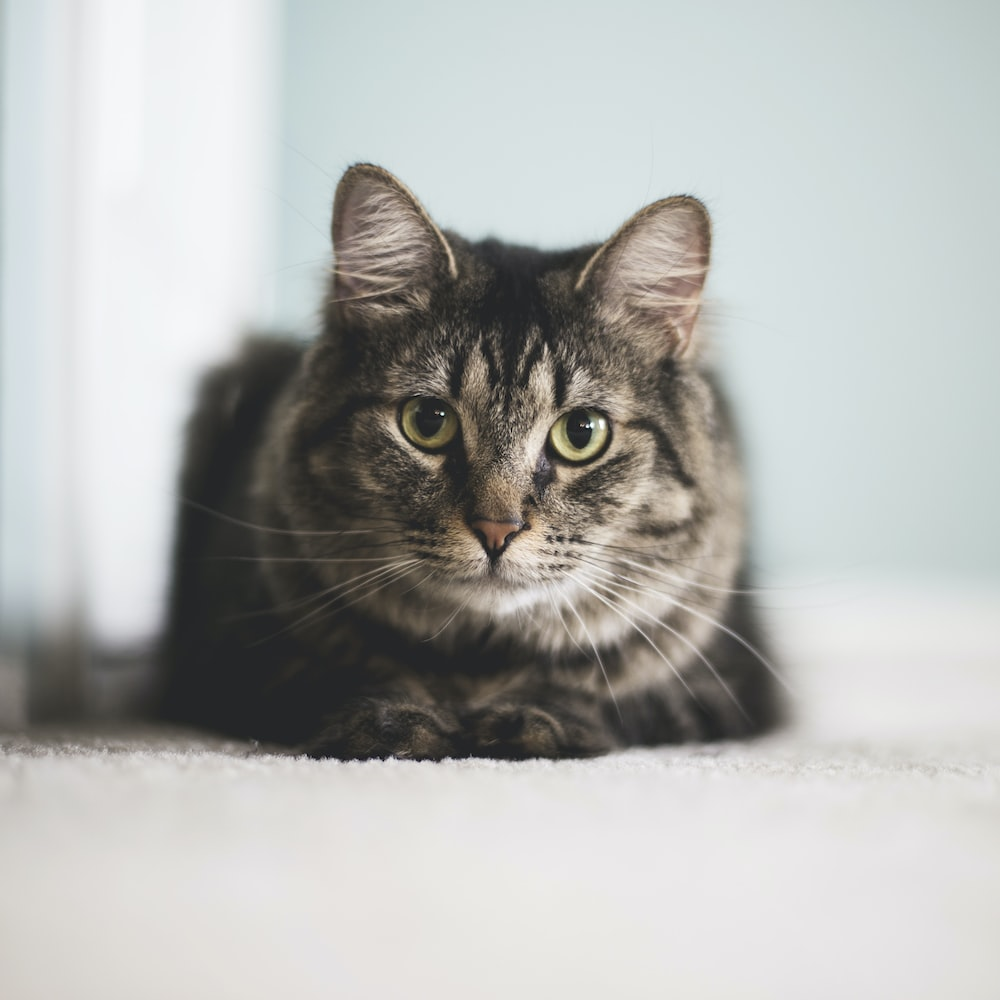
\includegraphics[width=1.5cm]{data/cat.jpeg}
			};
		\end{tikzpicture}
	\end{frame}

	\begin{frame}{Historien bak kunstig intelligens} %DL (imagenet)
		\begin{tikzpicture}
			\node[] at (0, 0) {};
			\node[] at (10.5, -7.5) {};

			\draw[very thick, gray] (0.5, -1)  -- (8.84, -1) {};

			\node[
				circle,
				draw=passivehistory,
				fill=passivehistory
			] at (1.65, -1) {};
			\node[
				anchor=north,
				passivehistory,
				align=center,
				font=\small\linespread{0.9}\selectfont,
				text height=9pt,
				text depth=3pt,
				inner sep=0pt,
				align=center
			] at (1.65, -1.588) {Turing-\\testen\\(1950)};

			\node[
				circle,
				draw=passivehistory,
				fill=passivehistory,
			] at (2.35, -1) {};
			\node[
				anchor=south,
				passivehistory,
				font=\small\linespread{0.9}\selectfont,
				text height=9pt,
				text depth=3pt,
				inner sep=0pt,
				align=center
			] at (2.35, -0.87) {Dartmouth\\(1956)};

			\node[
				circle,
				draw=passivehistory,
				fill=passivehistory,
			] at (2.68, -1) {};
			\node[
				anchor=north,
				passivehistory,
				font=\small\linespread{0.9}\selectfont,
				text height=9pt,
				text depth=3pt,
				inner sep=0pt,
				align=center
			] at (2.68, -1.375) {Perceptron\\(1958)};

			\node[
				circle,
				draw=passivehistory,
				fill=passivehistory
			] at (3.28, -1) {};
			\node[
				circle,
				draw=passivehistory,
				fill=passivehistory,
			] at (2.35, -1) {};
			\node[
				anchor=south,
				passivehistory,
				font=\small\linespread{0.9}\selectfont,
				text height=9pt,
				text depth=3pt,
				inner sep=0pt,
				align=center
			] at (3.28, -0.87) {Eliza\\(1964)};

			\node[
				circle,
				draw=passivehistory,
				fill=passivehistory
			] at (5.13, -1) {};
			\node[
				anchor=north,
				passivehistory,
				font=\small\linespread{0.9}\selectfont,
				text height=9pt,
				text depth=3pt,
				inner sep=0pt,
				align=center
			] at (5.13, -1.625) {Ekspert-\\systemer\\(1980s)};

			\node[
				circle,
				draw=passivehistory,
				fill=passivehistory
			] at (5.82, -1) {};
			\node[
				anchor=south,
				passivehistory,
				font=\small\linespread{0.9}\selectfont,
				text height=9pt,
				text depth=3pt,
				inner sep=0pt,
				align=center
			] at (5.82, -0.87) {ANN\\(1986)};

			\node[
				circle,
				draw=passivehistory,
				fill=passivehistory
			] at (7.10, -1) {};
			\node[
				anchor=north,
				passivehistory,
				font=\small\linespread{0.9}\selectfont,
				text height=9pt,
				text depth=3pt,
				inner sep=0pt,
				align=center
			] at (7.10, -1.372) {Deep blue\\(1997)};

			\node[
				circle,
				draw=activehistory,
				fill=activehistory
			] at (8.84, -1) {};
			\node[
				anchor=south,
				activehistory,
				font=\small\linespread{0.9}\selectfont,
				text height=9pt,
				text depth=3pt,
				inner sep=0pt,
				align=center
			] at (8.84, -0.87) {Deep learning\\(2012)};

			\node[inner sep=0pt, label=below:\small{Katt}] (img3) at (5.25, -4.75) {
				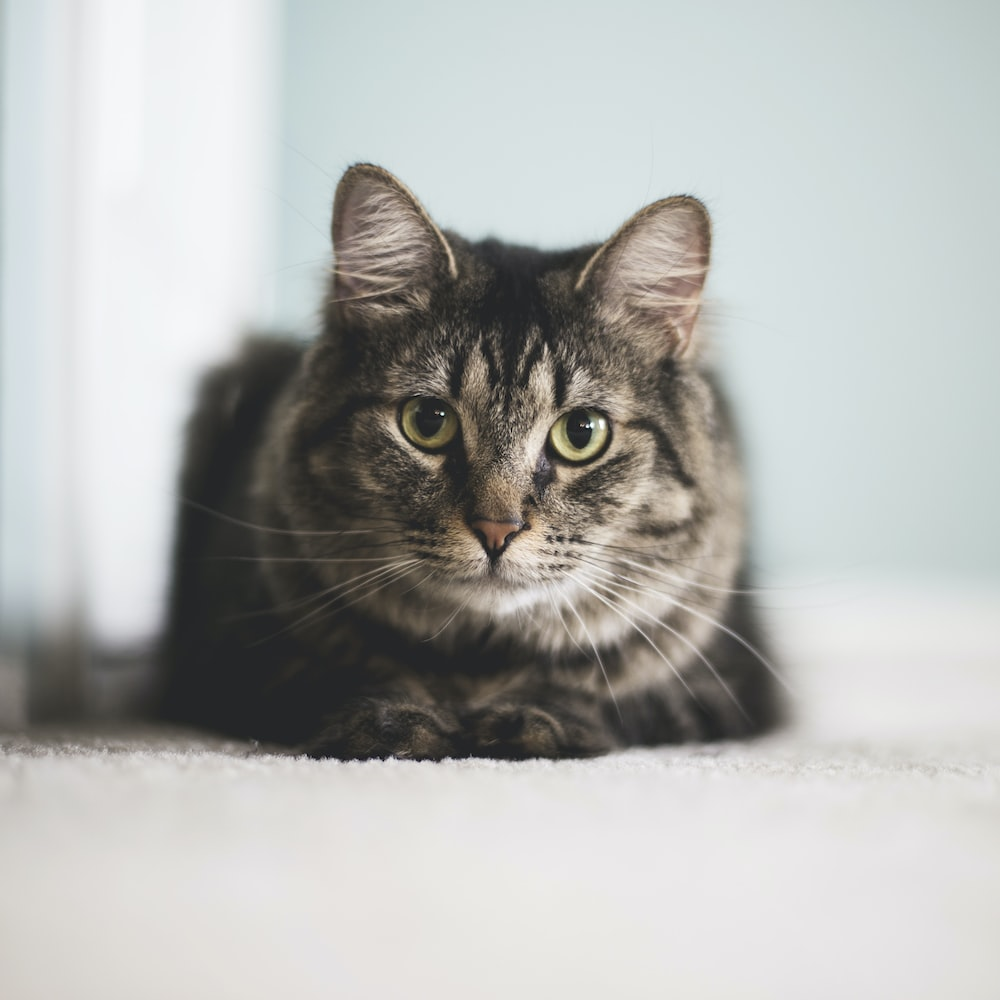
\includegraphics[width=1.5cm]{data/cat.jpeg}
			};
			\node[inner sep=0pt, label=below:\small{Fly}, anchor=west] (img4) at ($ (img3.east) + (0.1, 0) $) {
				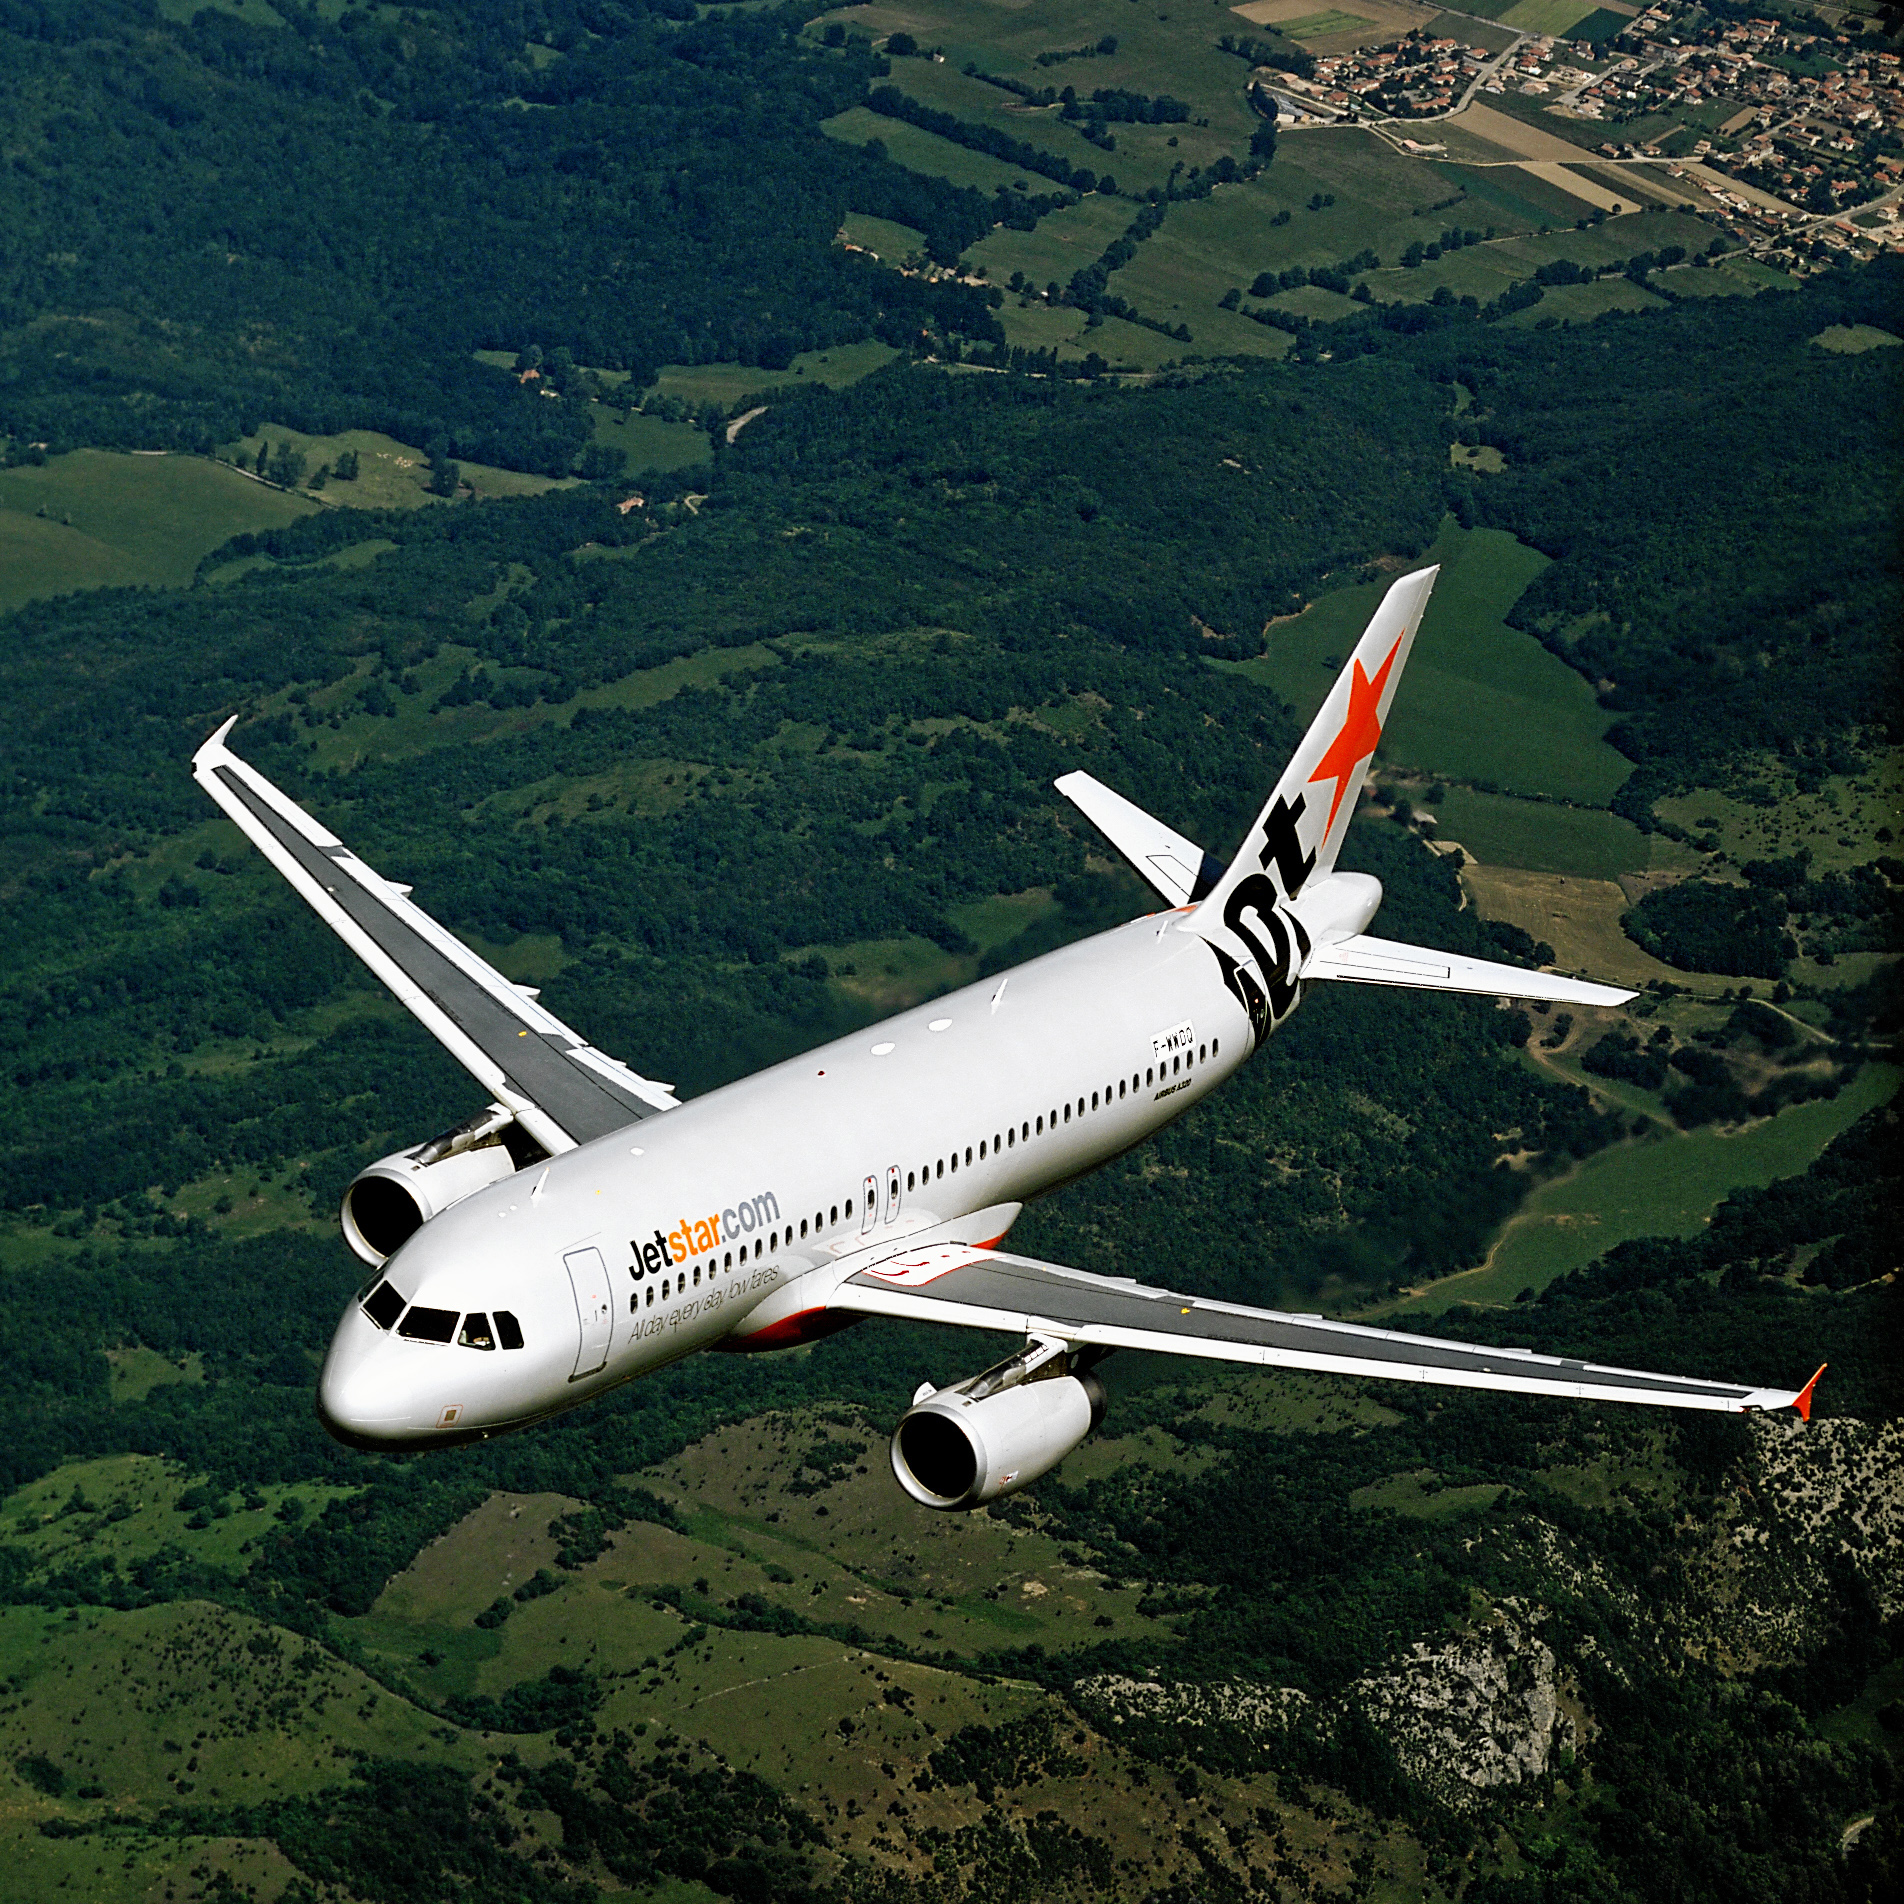
\includegraphics[width=1.5cm]{data/airplane.jpeg}
			};
			\node[inner sep=0pt, label=below:\small{Hvithai}, anchor=west] (img5) at ($ (img4.east) + (0.1, 0) $) {
				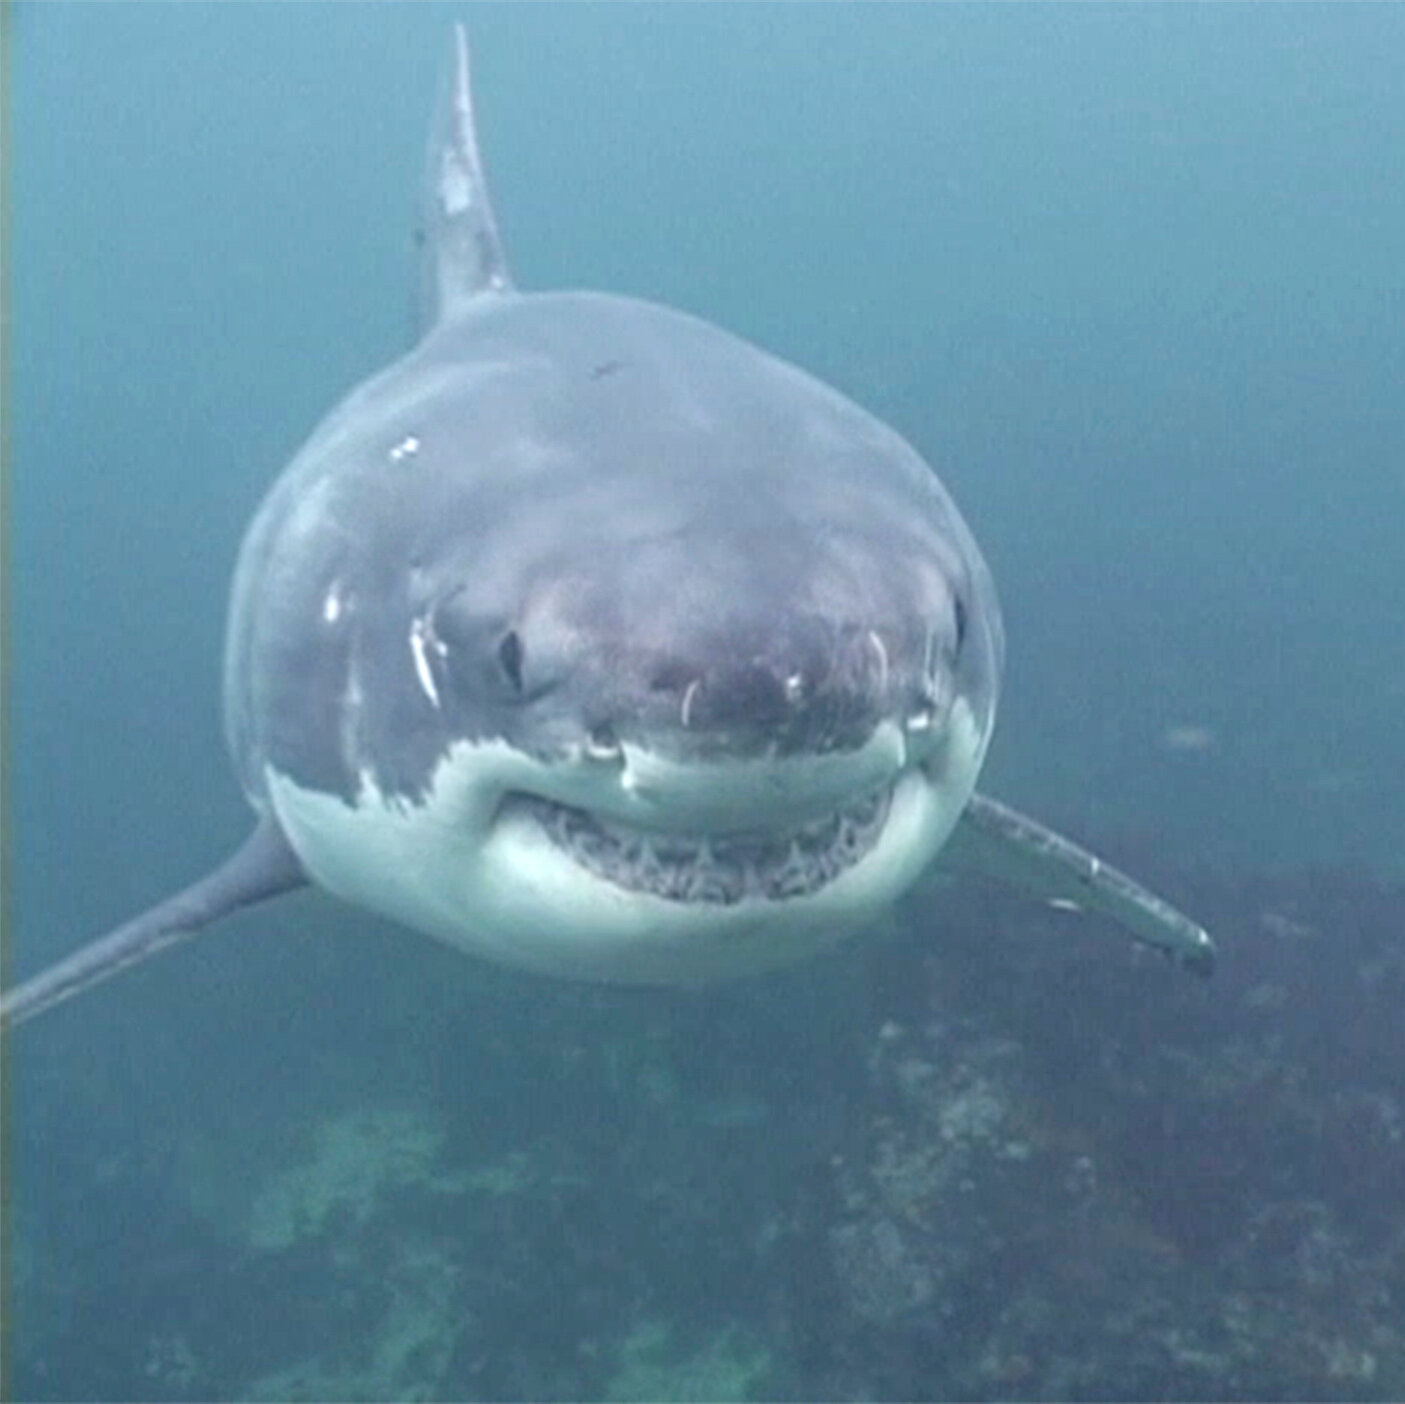
\includegraphics[width=1.5cm]{data/shark.jpeg}
			};
			\node[inner sep=0pt, label=below:\small{Marihøne}, anchor=east] (img2) at ($ (img3.west) - (0.1, 0) $) {
				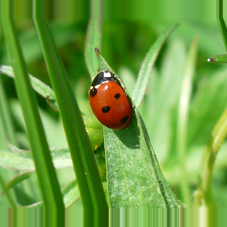
\includegraphics[width=1.5cm]{data/ladybug.png}
			};
			\node[inner sep=0pt, label=below:\small{Solsikke}, anchor=east] (img1) at ($ (img2.west) - (0.1, 0) $) {
				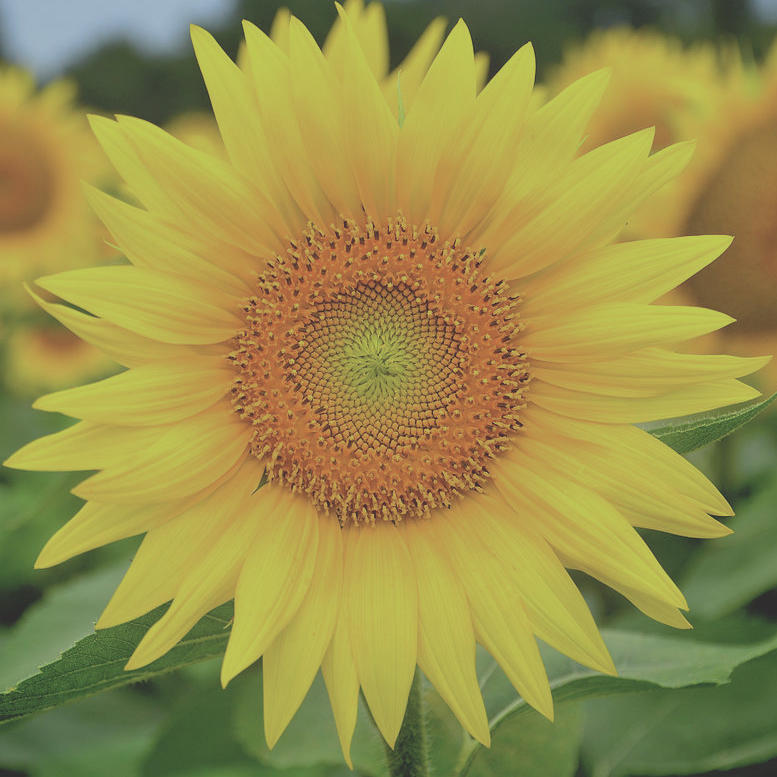
\includegraphics[width=1.5cm]{data/sunflower.jpeg}
			};
			\node[] at (5.25, -6.5) {
				ImageNet: $\sim$14m bilder, $\sim$22k kategorier
			};
		\end{tikzpicture}
	\end{frame}

	\begin{frame}{Historien bak kunstig intelligens} %DL (old)
		\newsavebox{\imagenetold}
		\sbox{\imagenetold}{%
			\begin{tikzpicture}
				\begin{axis}[
					ylabel={Feilrate},
					xlabel={År},
					xtick={2010, 2012, 2014, 2016, 2018, 2020},
					xticklabels={2010, 2012, 2014, 2016, 2018, 2020},
					ytick={0, 10, 20, 30},
					yticklabels={0\%, 10\%, 20\%, 30\%},
					ytick style={draw=none},
					ytick pos=left,
					xtick pos=bottom,
					ymajorgrids=true,
					ymax=29,
					ymin=0,
					xmin=2009,
					xmax=2021,
					width=8cm,
					height=5cm
				]
					\addplot[mark=*, purple,thick] coordinates {
						(2010, 28.2)
						(2011, 25.8)
					};

					\node[anchor=north, inner sep=5pt] at (axis cs: 2010, 28.2) {
						\small{28.2}
					};
					\node[anchor=north, inner sep=5pt] at (axis cs: 2011, 25.8) {
						\small{25.8}
					};
				\end{axis}
			\end{tikzpicture}
		}

		\begin{tikzpicture}
			\node[] at (0, 0) {};
			\node[] at (10.5, -7.5) {};

			\draw[very thick, gray] (0.5, -1)  -- (8.84, -1) {};

			\node[
				circle,
				draw=passivehistory,
				fill=passivehistory
			] at (1.65, -1) {};
			\node[
				anchor=north,
				passivehistory,
				align=center,
				font=\small\linespread{0.9}\selectfont,
				text height=9pt,
				text depth=3pt,
				inner sep=0pt,
				align=center
			] at (1.65, -1.588) {Turing-\\testen\\(1950)};

			\node[
				circle,
				draw=passivehistory,
				fill=passivehistory,
			] at (2.35, -1) {};
			\node[
				anchor=south,
				passivehistory,
				font=\small\linespread{0.9}\selectfont,
				text height=9pt,
				text depth=3pt,
				inner sep=0pt,
				align=center
			] at (2.35, -0.87) {Dartmouth\\(1956)};

			\node[
				circle,
				draw=passivehistory,
				fill=passivehistory,
			] at (2.68, -1) {};
			\node[
				anchor=north,
				passivehistory,
				font=\small\linespread{0.9}\selectfont,
				text height=9pt,
				text depth=3pt,
				inner sep=0pt,
				align=center
			] at (2.68, -1.375) {Perceptron\\(1958)};

			\node[
				circle,
				draw=passivehistory,
				fill=passivehistory
			] at (3.28, -1) {};
			\node[
				circle,
				draw=passivehistory,
				fill=passivehistory,
			] at (2.35, -1) {};
			\node[
				anchor=south,
				passivehistory,
				font=\small\linespread{0.9}\selectfont,
				text height=9pt,
				text depth=3pt,
				inner sep=0pt,
				align=center
			] at (3.28, -0.87) {Eliza\\(1964)};

			\node[
				circle,
				draw=passivehistory,
				fill=passivehistory
			] at (5.13, -1) {};
			\node[
				anchor=north,
				passivehistory,
				font=\small\linespread{0.9}\selectfont,
				text height=9pt,
				text depth=3pt,
				inner sep=0pt,
				align=center
			] at (5.13, -1.625) {Ekspert-\\systemer\\(1980s)};

			\node[
				circle,
				draw=passivehistory,
				fill=passivehistory
			] at (5.82, -1) {};
			\node[
				anchor=south,
				passivehistory,
				font=\small\linespread{0.9}\selectfont,
				text height=9pt,
				text depth=3pt,
				inner sep=0pt,
				align=center
			] at (5.82, -0.87) {ANN\\(1986)};

			\node[
				circle,
				draw=passivehistory,
				fill=passivehistory
			] at (7.10, -1) {};
			\node[
				anchor=north,
				passivehistory,
				font=\small\linespread{0.9}\selectfont,
				text height=9pt,
				text depth=3pt,
				inner sep=0pt,
				align=center
			] at (7.10, -1.372) {Deep blue\\(1997)};

			\node[
				circle,
				draw=activehistory,
				fill=activehistory
			] at (8.84, -1) {};
			\node[
				anchor=south,
				activehistory,
				font=\small\linespread{0.9}\selectfont,
				text height=9pt,
				text depth=3pt,
				inner sep=0pt,
				align=center
			] at (8.84, -0.87) {Deep learning\\(2012)};

			\node[inner sep=0pt] at (5.25, -4.75) {
				\usebox{\imagenetold}
			};
		\end{tikzpicture}
	\end{frame}

	\begin{frame}{Historien bak kunstig intelligens} %DL (CNN)
		\newsavebox{\imagenetcnn}
		\sbox{\imagenetcnn}{%
			\begin{tikzpicture}
				\begin{axis}[
					ylabel={Feilate},
					xlabel={År},
					xtick={2010, 2012, 2014, 2016, 2018, 2020},
					xticklabels={2010, 2012, 2014, 2016, 2018, 2020},
					ytick={0, 10, 20, 30},
					yticklabels={0\%, 10\%, 20\%, 30\%},
					ytick style={draw=none},
					ytick pos=left,
					xtick pos=bottom,
					ymajorgrids=true,
					ymax=29,
					ymin=0,
					xmin=2009,
					xmax=2021,
					width=8cm,
					height=5cm
				]
					\addplot[mark=*, purple,thick] coordinates {
						(2010, 28.2)
						(2011, 25.8)
						(2012, 16.4)
					};

					\node[anchor=north, inner sep=5pt] at (axis cs: 2010, 28.2) {
						\small{28.2}
					};
					\node[anchor=north, inner sep=5pt] at (axis cs: 2011, 25.8) {
						\small{25.8}
					};
					\node[anchor=north, inner sep=5pt] at (axis cs: 2012, 16.4) {
						\small{16.4}
					};

					\addplot[densely dotted] coordinates {
						(2011.5, 30)
						(2011.5, 0)
					};
				\end{axis}
			\end{tikzpicture}
		}

		\begin{tikzpicture}
			\node[] at (0, 0) {};
			\node[] at (10.5, -7.5) {};

			\draw[very thick, gray] (0.5, -1)  -- (8.84, -1) {};

			\node[
				circle,
				draw=passivehistory,
				fill=passivehistory
			] at (1.65, -1) {};
			\node[
				anchor=north,
				passivehistory,
				align=center,
				font=\small\linespread{0.9}\selectfont,
				text height=9pt,
				text depth=3pt,
				inner sep=0pt,
				align=center
			] at (1.65, -1.588) {Turing-\\testen\\(1950)};

			\node[
				circle,
				draw=passivehistory,
				fill=passivehistory,
			] at (2.35, -1) {};
			\node[
				anchor=south,
				passivehistory,
				font=\small\linespread{0.9}\selectfont,
				text height=9pt,
				text depth=3pt,
				inner sep=0pt,
				align=center
			] at (2.35, -0.87) {Dartmouth\\(1956)};

			\node[
				circle,
				draw=passivehistory,
				fill=passivehistory,
			] at (2.68, -1) {};
			\node[
				anchor=north,
				passivehistory,
				font=\small\linespread{0.9}\selectfont,
				text height=9pt,
				text depth=3pt,
				inner sep=0pt,
				align=center
			] at (2.68, -1.375) {Perceptron\\(1958)};

			\node[
				circle,
				draw=passivehistory,
				fill=passivehistory
			] at (3.28, -1) {};
			\node[
				circle,
				draw=passivehistory,
				fill=passivehistory,
			] at (2.35, -1) {};
			\node[
				anchor=south,
				passivehistory,
				font=\small\linespread{0.9}\selectfont,
				text height=9pt,
				text depth=3pt,
				inner sep=0pt,
				align=center
			] at (3.28, -0.87) {Eliza\\(1964)};

			\node[
				circle,
				draw=passivehistory,
				fill=passivehistory
			] at (5.13, -1) {};
			\node[
				anchor=north,
				passivehistory,
				font=\small\linespread{0.9}\selectfont,
				text height=9pt,
				text depth=3pt,
				inner sep=0pt,
				align=center
			] at (5.13, -1.625) {Ekspert-\\systemer\\(1980s)};

			\node[
				circle,
				draw=passivehistory,
				fill=passivehistory
			] at (5.82, -1) {};
			\node[
				anchor=south,
				passivehistory,
				font=\small\linespread{0.9}\selectfont,
				text height=9pt,
				text depth=3pt,
				inner sep=0pt,
				align=center
			] at (5.82, -0.87) {ANN\\(1986)};

			\node[
				circle,
				draw=passivehistory,
				fill=passivehistory
			] at (7.10, -1) {};
			\node[
				anchor=north,
				passivehistory,
				font=\small\linespread{0.9}\selectfont,
				text height=9pt,
				text depth=3pt,
				inner sep=0pt,
				align=center
			] at (7.10, -1.372) {Deep blue\\(1997)};

			\node[
				circle,
				draw=activehistory,
				fill=activehistory
			] at (8.84, -1) {};
			\node[
				anchor=south,
				activehistory,
				font=\small\linespread{0.9}\selectfont,
				text height=9pt,
				text depth=3pt,
				inner sep=0pt,
				align=center
			] at (8.84, -0.87) {Deep learning\\(2012)};

			\node[inner sep=0pt] at (5.25, -4.75) {
				\usebox{\imagenetcnn}
			};
		\end{tikzpicture}
	\end{frame}

	\begin{frame}{Historien bak kunstig intelligens} %DL (2020)
		\newsavebox{\imagenetlatest}
		\sbox{\imagenetlatest}{%
			\begin{tikzpicture}
				\begin{axis}[
					ylabel={Feilrate},
					xlabel={År},
					xtick={2010, 2012, 2014, 2016, 2018, 2020},
					xticklabels={2010, 2012, 2014, 2016, 2018, 2020},
					ytick={0, 10, 20, 30},
					yticklabels={0\%, 10\%, 20\%, 30\%},
					ytick style={draw=none},
					ytick pos=left,
					xtick pos=bottom,
					ymajorgrids=true,
					ymax=29,
					ymin=0,
					xmin=2009,
					xmax=2021,
					width=8cm,
					height=5cm
				]
					\addplot[mark=*, purple,thick] coordinates {
						(2010, 28.2)
						(2011, 25.8)
						(2012, 16.4)
						(2013, 11.7)
						(2014, 7.3)
						(2015, 3.5)
						(2016, 3.0)
						(2017, 2.3)
						(2018, 1.8)
						(2019, 1.3)
						(2020, 0.9)
					};

					\node[anchor=north, inner sep=5pt] at (axis cs: 2010, 28.2) {
						\small{28.2}
					};
					\node[anchor=north, inner sep=5pt] at (axis cs: 2011, 25.8) {
						\small{25.8}
					};
					\node[anchor=north, inner sep=5pt] at (axis cs: 2012, 16.4) {
						\small{16.4}
					};
					\node[anchor=north, inner sep=5pt] at (axis cs: 2013, 11.7) {
						\small{11.7}
					};
					\node[anchor=north, inner sep=5pt] at (axis cs: 2014, 7.3) {
						\small{7.3}
					};
					\node[anchor=north, inner sep=5pt] at (axis cs: 2015, 3.5) {
						\small{3.5}
					};
					\node[anchor=south, inner sep=5pt] at (axis cs: 2016, 3.0) {
						\small{3.0}
					};
					\node[anchor=south, inner sep=5pt] at (axis cs: 2017, 2.3) {
						\small{2.3}
					};
					\node[anchor=south, inner sep=5pt] at (axis cs: 2018, 1.8) {
						\small{1.8}
					};
					\node[anchor=south, inner sep=5pt] at (axis cs: 2019, 1.3) {
						\small{1.3}
					};
					\node[anchor=south, inner sep=5pt] at (axis cs: 2020, 0.9) {
						\small{\textbf{0.9}}
					};

					\addplot[densely dotted] coordinates {
						(2011.5, 30)
						(2011.5, 0)
					};
				\end{axis}
			\end{tikzpicture}
		}

		\begin{tikzpicture}
			\node[] at (0, 0) {};
			\node[] at (10.5, -7.5) {};

			\draw[very thick, gray] (0.5, -1)  -- (8.84, -1) {};

			\node[
				circle,
				draw=passivehistory,
				fill=passivehistory
			] at (1.65, -1) {};
			\node[
				anchor=north,
				passivehistory,
				align=center,
				font=\small\linespread{0.9}\selectfont,
				text height=9pt,
				text depth=3pt,
				inner sep=0pt,
				align=center
			] at (1.65, -1.588) {Turing-\\testen\\(1950)};

			\node[
				circle,
				draw=passivehistory,
				fill=passivehistory,
			] at (2.35, -1) {};
			\node[
				anchor=south,
				passivehistory,
				font=\small\linespread{0.9}\selectfont,
				text height=9pt,
				text depth=3pt,
				inner sep=0pt,
				align=center
			] at (2.35, -0.87) {Dartmouth\\(1956)};

			\node[
				circle,
				draw=passivehistory,
				fill=passivehistory,
			] at (2.68, -1) {};
			\node[
				anchor=north,
				passivehistory,
				font=\small\linespread{0.9}\selectfont,
				text height=9pt,
				text depth=3pt,
				inner sep=0pt,
				align=center
			] at (2.68, -1.375) {Perceptron\\(1958)};

			\node[
				circle,
				draw=passivehistory,
				fill=passivehistory
			] at (3.28, -1) {};
			\node[
				circle,
				draw=passivehistory,
				fill=passivehistory,
			] at (2.35, -1) {};
			\node[
				anchor=south,
				passivehistory,
				font=\small\linespread{0.9}\selectfont,
				text height=9pt,
				text depth=3pt,
				inner sep=0pt,
				align=center
			] at (3.28, -0.87) {Eliza\\(1964)};

			\node[
				circle,
				draw=passivehistory,
				fill=passivehistory
			] at (5.13, -1) {};
			\node[
				anchor=north,
				passivehistory,
				font=\small\linespread{0.9}\selectfont,
				text height=9pt,
				text depth=3pt,
				inner sep=0pt,
				align=center
			] at (5.13, -1.625) {Ekspert-\\systemer\\(1980s)};

			\node[
				circle,
				draw=passivehistory,
				fill=passivehistory
			] at (5.82, -1) {};
			\node[
				anchor=south,
				passivehistory,
				font=\small\linespread{0.9}\selectfont,
				text height=9pt,
				text depth=3pt,
				inner sep=0pt,
				align=center
			] at (5.82, -0.87) {ANN\\(1986)};

			\node[
				circle,
				draw=passivehistory,
				fill=passivehistory
			] at (7.10, -1) {};
			\node[
				anchor=north,
				passivehistory,
				font=\small\linespread{0.9}\selectfont,
				text height=9pt,
				text depth=3pt,
				inner sep=0pt,
				align=center
			] at (7.10, -1.372) {Deep blue\\(1997)};

			\node[
				circle,
				draw=activehistory,
				fill=activehistory
			] at (8.84, -1) {};
			\node[
				anchor=south,
				activehistory,
				font=\small\linespread{0.9}\selectfont,
				text height=9pt,
				text depth=3pt,
				inner sep=0pt,
				align=center
			] at (8.84, -0.87) {Deep learning\\(2012)};

			\node[inner sep=0pt] at (5.25, -4.75) {
				\usebox{\imagenetlatest}
			};
		\end{tikzpicture}
	\end{frame}

	\begin{frame}{Historien bak kunstig intelligens} %DL (human)
		\newsavebox{\imagenethuman}
		\sbox{\imagenethuman}{%
			\begin{tikzpicture}
				\begin{axis}[
					ylabel={Feilrate},
					xlabel={År},
					xtick={2010, 2012, 2014, 2016, 2018, 2020},
					xticklabels={2010, 2012, 2014, 2016, 2018, 2020},
					ytick={0, 10, 20, 30},
					yticklabels={0\%, 10\%, 20\%, 30\%},
					ytick style={draw=none},
					ytick pos=left,
					xtick pos=bottom,
					ymajorgrids=true,
					ymax=29,
					ymin=0,
					xmin=2009,
					xmax=2021,
					width=8cm,
					height=5cm
				]
					\addplot[mark=*, purple,thick] coordinates {
						(2010, 28.2)
						(2011, 25.8)
						(2012, 16.4)
						(2013, 11.7)
						(2014, 7.3)
						(2015, 3.5)
						(2016, 3.0)
						(2017, 2.3)
						(2018, 1.8)
						(2019, 1.3)
						(2020, 0.9)
					};

					\node[anchor=north, inner sep=5pt] at (axis cs: 2010, 28.2) {
						\small{28.2}
					};
					\node[anchor=north, inner sep=5pt] at (axis cs: 2011, 25.8) {
						\small{25.8}
					};
					\node[anchor=north, inner sep=5pt] at (axis cs: 2012, 16.4) {
						\small{16.4}
					};
					\node[anchor=north, inner sep=5pt] at (axis cs: 2013, 11.7) {
						\small{11.7}
					};
					\node[anchor=north, inner sep=5pt] at (axis cs: 2014, 7.3) {
						\small{7.3}
					};
					\node[anchor=north, inner sep=5pt] at (axis cs: 2015, 3.5) {
						\small{3.5}
					};
					\node[anchor=south, inner sep=5pt] at (axis cs: 2016, 3.0) {
						\small{3.0}
					};
					\node[anchor=south, inner sep=5pt] at (axis cs: 2017, 2.3) {
						\small{2.3}
					};
					\node[anchor=south, inner sep=5pt] at (axis cs: 2018, 1.8) {
						\small{1.8}
					};
					\node[anchor=south, inner sep=5pt] at (axis cs: 2019, 1.3) {
						\small{1.3}
					};
					\node[anchor=south, inner sep=5pt] at (axis cs: 2020, 0.9) {
						\small{\textbf{0.9}}
					};

					\addplot[densely dotted] coordinates {
						(2011.5, 30)
						(2011.5, 0)
					};

					\addplot[dashed, red] coordinates {
						(2009, 5.1)
						(2021, 5.1)
					};

					\node[anchor=south east] at (axis cs: 2021, 5.1) {
						\textcolor{red}{\small{Menneskelig nivå}}
					};
				\end{axis}
			\end{tikzpicture}
		}

		\begin{tikzpicture}
			\node[] at (0, 0) {};
			\node[] at (10.5, -7.5) {};

			\draw[very thick, gray] (0.5, -1)  -- (8.84, -1) {};

			\node[
				circle,
				draw=passivehistory,
				fill=passivehistory
			] at (1.65, -1) {};
			\node[
				anchor=north,
				passivehistory,
				align=center,
				font=\small\linespread{0.9}\selectfont,
				text height=9pt,
				text depth=3pt,
				inner sep=0pt,
				align=center
			] at (1.65, -1.588) {Turing-\\testen\\(1950)};

			\node[
				circle,
				draw=passivehistory,
				fill=passivehistory,
			] at (2.35, -1) {};
			\node[
				anchor=south,
				passivehistory,
				font=\small\linespread{0.9}\selectfont,
				text height=9pt,
				text depth=3pt,
				inner sep=0pt,
				align=center
			] at (2.35, -0.87) {Dartmouth\\(1956)};

			\node[
				circle,
				draw=passivehistory,
				fill=passivehistory,
			] at (2.68, -1) {};
			\node[
				anchor=north,
				passivehistory,
				font=\small\linespread{0.9}\selectfont,
				text height=9pt,
				text depth=3pt,
				inner sep=0pt,
				align=center
			] at (2.68, -1.375) {Perceptron\\(1958)};

			\node[
				circle,
				draw=passivehistory,
				fill=passivehistory
			] at (3.28, -1) {};
			\node[
				circle,
				draw=passivehistory,
				fill=passivehistory,
			] at (2.35, -1) {};
			\node[
				anchor=south,
				passivehistory,
				font=\small\linespread{0.9}\selectfont,
				text height=9pt,
				text depth=3pt,
				inner sep=0pt,
				align=center
			] at (3.28, -0.87) {Eliza\\(1964)};

			\node[
				circle,
				draw=passivehistory,
				fill=passivehistory
			] at (5.13, -1) {};
			\node[
				anchor=north,
				passivehistory,
				font=\small\linespread{0.9}\selectfont,
				text height=9pt,
				text depth=3pt,
				inner sep=0pt,
				align=center
			] at (5.13, -1.625) {Ekspert-\\systemer\\(1980s)};

			\node[
				circle,
				draw=passivehistory,
				fill=passivehistory
			] at (5.82, -1) {};
			\node[
				anchor=south,
				passivehistory,
				font=\small\linespread{0.9}\selectfont,
				text height=9pt,
				text depth=3pt,
				inner sep=0pt,
				align=center
			] at (5.82, -0.87) {ANN\\(1986)};

			\node[
				circle,
				draw=passivehistory,
				fill=passivehistory
			] at (7.10, -1) {};
			\node[
				anchor=north,
				passivehistory,
				font=\small\linespread{0.9}\selectfont,
				text height=9pt,
				text depth=3pt,
				inner sep=0pt,
				align=center
			] at (7.10, -1.372) {Deep blue\\(1997)};

			\node[
				circle,
				draw=activehistory,
				fill=activehistory
			] at (8.84, -1) {};
			\node[
				anchor=south,
				activehistory,
				font=\small\linespread{0.9}\selectfont,
				text height=9pt,
				text depth=3pt,
				inner sep=0pt,
				align=center
			] at (8.84, -0.87) {Deep learning\\(2012)};

			\node[inner sep=0pt] at (5.25, -4.75) {
				\usebox{\imagenethuman}
			};
		\end{tikzpicture}
	\end{frame}

	\begin{frame}{Historien bak kunstig intelligens} %ChatGPT
		\begin{tikzpicture}
			\node[] at (0, 0) {};
			\node[] at (10.5, -7.5) {};

			\draw[very thick, gray] (0.5, -1)  -- (10, -1) {};

			\node[
				circle,
				draw=passivehistory,
				fill=passivehistory
			] at (1.65, -1) {};
			\node[
				anchor=north,
				passivehistory,
				align=center,
				font=\small\linespread{0.9}\selectfont,
				text height=9pt,
				text depth=3pt,
				inner sep=0pt,
				align=center
			] at (1.65, -1.588) {Turing-\\testen\\(1950)};

			\node[
				circle,
				draw=passivehistory,
				fill=passivehistory,
			] at (2.35, -1) {};
			\node[
				anchor=south,
				passivehistory,
				font=\small\linespread{0.9}\selectfont,
				text height=9pt,
				text depth=3pt,
				inner sep=0pt,
				align=center
			] at (2.35, -0.87) {Dartmouth\\(1956)};

			\node[
				circle,
				draw=passivehistory,
				fill=passivehistory,
			] at (2.68, -1) {};
			\node[
				anchor=north,
				passivehistory,
				font=\small\linespread{0.9}\selectfont,
				text height=9pt,
				text depth=3pt,
				inner sep=0pt,
				align=center
			] at (2.68, -1.375) {Perceptron\\(1958)};

			\node[
				circle,
				draw=passivehistory,
				fill=passivehistory
			] at (3.28, -1) {};
			\node[
				circle,
				draw=passivehistory,
				fill=passivehistory,
			] at (2.35, -1) {};
			\node[
				anchor=south,
				passivehistory,
				font=\small\linespread{0.9}\selectfont,
				text height=9pt,
				text depth=3pt,
				inner sep=0pt,
				align=center
			] at (3.28, -0.87) {Eliza\\(1964)};

			\node[
				circle,
				draw=passivehistory,
				fill=passivehistory
			] at (5.13, -1) {};
			\node[
				anchor=north,
				passivehistory,
				font=\small\linespread{0.9}\selectfont,
				text height=9pt,
				text depth=3pt,
				inner sep=0pt,
				align=center
			] at (5.13, -1.625) {Ekspert-\\systemer\\(1980s)};

			\node[
				circle,
				draw=passivehistory,
				fill=passivehistory
			] at (5.82, -1) {};
			\node[
				anchor=south,
				passivehistory,
				font=\small\linespread{0.9}\selectfont,
				text height=9pt,
				text depth=3pt,
				inner sep=0pt,
				align=center
			] at (5.82, -0.87) {ANN\\(1986)};

			\node[
				circle,
				draw=passivehistory,
				fill=passivehistory
			] at (7.10, -1) {};
			\node[
				anchor=north,
				passivehistory,
				font=\small\linespread{0.9}\selectfont,
				text height=9pt,
				text depth=3pt,
				inner sep=0pt,
				align=center
			] at (7.10, -1.372) {Deep blue\\(1997)};

			\node[
				circle,
				draw=passivehistory,
				fill=passivehistory
			] at (8.84, -1) {};
			\node[
				anchor=south,
				passivehistory,
				font=\small\linespread{0.9}\selectfont,
				text height=9pt,
				text depth=3pt,
				inner sep=0pt,
				align=center
			] at (8.84, -0.87) {Deep learning\\(2012)};

			\node[
				circle,
				draw=activehistory,
				fill=activehistory
			] at (10, -1) {};
			\node[
				anchor=north,
				activehistory,
				font=\small\linespread{0.9}\selectfont,
				text height=9pt,
				text depth=3pt,
				inner sep=0pt,
				align=center
			] at (10, -1.33) {ChatGPT\\(2022)};

			\node[inner sep=0pt, draw=black] at (5.25, -4.75) {
				
\includegraphics[width=6cm]{data/chatgpt.png}
			};
		\end{tikzpicture}
	\end{frame}

	\section{Terminologi og konsepter}

	\begin{frame}{Terminologi og konsepter: Begreper} % Taxonomy, Artificial intelligence
		\centering
		\vfill
		\begin{tikzpicture}
			\node[circle, fill=blue!60, minimum size=6cm] (ai) at (0, 0) {};
			\node[text=white, anchor=north] at ($ (ai.north) - (0, 0.3) $) {\textbf{Kunstig intelligens}};
			\node[anchor=north west, align=left, font=\small] (ai-text) at ($ (ai.north) + (3.5, 0.2) $) {\textbf{Kunstig intelligens:}\\Maskiner som løser oppgaver\\som krever intelligens};
			\node[] at (-3, 3) {};
			\node[] at (7.7, -3.2) {};
		\end{tikzpicture}
		\vfill
	\end{frame}

	\begin{frame}{Terminologi og konsepter: Begreper} % Taxonomy, Symbolsk AI
		\centering
		\vfill
		\begin{tikzpicture}
			\node[circle, fill=blue!60, minimum size=6cm] (ai) at (0, 0) {};
			\node[text=white, anchor=north] at ($ (ai.north) - (0, 0.3) $) {\textbf{Kunstig intelligens}};
			\node[text=white] at ($ (ai.north) - (-1.1, 1.2) $) {Symbolsk AI};
			\node[anchor=north west, align=left, font=\small, text=gray!40] (ai-text) at ($ (ai.north) + (3.5, 0.2) $) {\textbf{Kunstig intelligens:}\\Maskiner som løser oppgaver\\som krever intelligens};

			\node[] at (-3, 3) {};
			\node[] at (7.7, -3.2) {};
		\end{tikzpicture}
		\vfill
	\end{frame}

	\begin{frame}{Terminologi og konsepter: Begreper} % Taxonomy, Machine learning explanation
		\centering
		\vfill
		\begin{tikzpicture}
			\node[circle, fill=blue!60, minimum size=6cm] (ai) at (0, 0) {};
			\node[text=white, anchor=north] at ($ (ai.north) - (0, 0.3) $) {\textbf{Kunstig intelligens}};
			\node[text=white] at ($ (ai.north) - (-1.1, 1.2) $) {Symbolsk AI};
			\node[circle, fill=purple!60, minimum size=4.5cm, anchor=south] (ml) at ($ (ai.south) + (0, 0.05) $) {};
			\node[text=white, anchor=north] at ($ (ml.north) - (0, 0.3) $) {\textbf{Maskinlæring}};
			\node[anchor=north west, align=left, font=\small, text=gray!40] (ai-text) at ($ (ai.north) + (3.5, 0.2) $) {\textbf{Kunstig intelligens:}\\Maskiner som løser oppgaver\\som krever intelligens};
			\node[anchor=north west, align=left, font=\small] (ml-text) at ($ (ai-text.south west) - (0, 0) $) {\textbf{Maskinlæring:}\\Maskiner som løser problemer\\gjennom å lære seg å finne\\mønster i data};
			\node[] at (-3, 3) {};
			\node[] at (7.7, -3.2) {};
		\end{tikzpicture}
		\vfill
	\end{frame}

	\begin{frame}{Terminologi og konsepter: Begreper} % Taxonomy, Deep learning
		\centering
		\vfill
		\begin{tikzpicture}
			\node[circle, fill=blue!60, minimum size=6cm] (ai) at (0, 0) {};
			\node[text=white, anchor=north] at ($ (ai.north) - (0, 0.3) $) {\textbf{Kunstig intelligens}};
			\node[text=white] at ($ (ai.north) - (-1.1, 1.2) $) {Symbolsk AI};
			\node[circle, fill=purple!60, minimum size=4.5cm, anchor=south] (ml) at ($ (ai.south) + (0, 0.05) $) {};
			\node[text=white, anchor=north] at ($ (ml.north) - (0, 0.3) $) {\textbf{Maskinlæring}};
			\node[text=white, align=center, font=\linespread{0.5}\selectfont] at ($ (ml.north) - (1, 1.1) $) {Lineær\\regresjon};
			\node[anchor=north west, align=left, font=\small, text=gray!40] (ai-text) at ($ (ai.north) + (3.5, 0.2) $) {\textbf{Kunstig intelligens:}\\Maskiner som løser oppgaver\\som krever intelligens};
			\node[anchor=north west, align=left, font=\small, text=gray!40] (ml-text) at ($ (ai-text.south west) - (0, 0) $) {\textbf{Maskinlæring:}\\Maskiner som løser problemer\\gjennom å lære seg å finne\\mønster i data};

			\node[] at (-3, 3) {};
			\node[] at (7.7, -3.2) {};
		\end{tikzpicture}
		\vfill
	\end{frame}

	\begin{frame}{Terminologi og konsepter: Begreper} % Taxonomy, Deep learning
		\centering
		\vfill
		\begin{tikzpicture}
			\node[circle, fill=blue!60, minimum size=6cm] (ai) at (0, 0) {};
			\node[text=white, anchor=north] at ($ (ai.north) - (0, 0.3) $) {\textbf{Kunstig intelligens}};
			\node[text=white] at ($ (ai.north) - (-1.1, 1.2) $) {Symbolsk AI};
			\node[circle, fill=purple!60, minimum size=4.5cm, anchor=south] (ml) at ($ (ai.south) + (0, 0.05) $) {};
			\node[text=white, anchor=north] at ($ (ml.north) - (0, 0.3) $) {\textbf{Maskinlæring}};
			\node[text=white, align=center, font=\linespread{0.5}\selectfont] at ($ (ml.north) - (1, 1.1) $) {Lineær\\regresjon};
			\node[circle, fill=red!60, minimum size=3cm, anchor=south] (dl) at ($ (ai.south) + (0, 0.1) $) {};
			\node[text=white, anchor=north] at ($ (dl.north) - (0, 0.3) $) {\textbf{Dyplæring}};
			\node[anchor=north west, align=left, font=\small, text=gray!40] (ai-text) at ($ (ai.north) + (3.5, 0.2) $) {\textbf{Kunstig intelligens:}\\Maskiner som løser oppgaver\\som krever intelligens};
			\node[anchor=north west, align=left, font=\small, text=gray!40] (ml-text) at ($ (ai-text.south west) - (0, 0) $) {\textbf{Maskinlæring:}\\Maskiner som løser problemer\\gjennom å lære seg å finne\\mønster i data};
			\node[anchor=north west, align=left, font=\small] (dl-text) at ($ (ml-text.south west) - (0, 0) $) {\textbf{Dyplæring:}\\Maskinlæringsmodeller som\\er organisert i hierarkier\\($\approx$ dype nevrale nettverk)\\inspirert av hjernen};
			\node[] at (-3, 3) {};
			\node[] at (7.7, -3.2) {};
		\end{tikzpicture}
		\vfill
	\end{frame}

	\begin{frame}{Terminologi og konsepter: Begreper} % Taxonomy, CNNs and LLMs
		\centering
		\vfill
		\begin{tikzpicture}
			\node[circle, fill=blue!60, minimum size=6cm] (ai) at (0, 0) {};
			\node[text=white, anchor=north] at ($ (ai.north) - (0, 0.3) $) {\textbf{Kunstig intelligens}};
			\node[text=white] at ($ (ai.north) - (-1.1, 1.2) $) {Symbolsk AI};
			\node[circle, fill=purple!60, minimum size=4.5cm, anchor=south] (ml) at ($ (ai.south) + (0, 0.05) $) {};
			\node[text=white, anchor=north] at ($ (ml.north) - (0, 0.3) $) {\textbf{Maskinlæring}};
			\node[text=white, align=center, font=\linespread{0.5}\selectfont] at ($ (ml.north) - (1, 1.1) $) {Lineær\\regresjon};
			\node[circle, fill=red!60, minimum size=3cm, anchor=south] (dl) at ($ (ai.south) + (0, 0.1) $) {};
			\node[text=white, anchor=north] at ($ (dl.north) - (0, 0.3) $) {\textbf{Dyplæring}};
			\node[align=center, text=white, font=\linespread{0.5}\selectfont] at ($ (dl.north) - (-0.2, 1.2) $) {Konvolusjonelle\\nevrale nettverk};
			\node[align=center, text=white, font=\linespread{0.5}\selectfont] at ($ (dl.north) - (0.2, 2.1) $) {Store\\språkmodeller};
			\node[anchor=north west, align=left, font=\small, text=gray!40] (ai-text) at ($ (ai.north) + (3.5, 0.2) $) {\textbf{Kunstig intelligens:}\\Maskiner som løser oppgaver\\som krever intelligens};
			\node[anchor=north west, align=left, font=\small, text=gray!40] (ml-text) at ($ (ai-text.south west) - (0, 0) $) {\textbf{Maskinlæring:}\\Maskiner som løser problemer\\gjennom å lære seg å finne\\mønster i data};
			\node[anchor=north west, align=left, font=\small, text=gray!40] (dl-text) at ($ (ml-text.south west) - (0, 0) $) {\textbf{Dyplæring:}\\Maskinlæringsmodeller som\\er organisert i hierarkier\\($\approx$ dype nevrale nettverk)\\inspirert av hjernen};
			\node[anchor=north west, align=left, font=\small] (cnn-text) at ($ (dl-text.south west) - (0, 0) $) {\textbf{Konvolusjonelle nevrale nettverk:}\\Nevrale nettverk for\\bildedata};
			\node[anchor=north west, align=left, font=\small] at ($ (cnn-text.south west) - (0, 0) $) {\textbf{Store språkmodeller:}\\Nevrale nettverk for\\språkdata (ChatGPT)};
			\node[] at (-3, 3) {};
			\node[] at (7.7, -3.2) {};
		\end{tikzpicture}
		\vfill
	\end{frame}

	\begin{frame}{Terminologi og konsepter: Veiledning} % Supervised vs unsupervised
		\centering
		\vfill
		\begin{tikzpicture}
			\node[align=center, anchor=north] (supervised) at (0, 0) {Veiledet læring\\(supervised learning)};
			\node[align=center, anchor=north] (unsupervised) at (7, 0) {Ikke-veiledet læring\\(unsupervised learning)};
			\draw[] (3.5, 0) -- (3.5, -7.5);
			\node[] (cat1) at ($ (supervised.south) + (-1, -0.8) $) {
				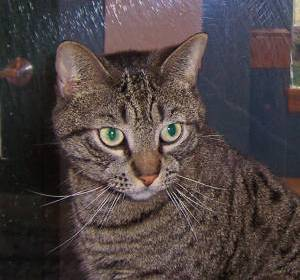
\includegraphics[width=1.2cm]{data/cat.1.jpg}
			};
			\node[anchor=west] (cattext1) at ($ (cat1.east) + (1.2, 0) $) {Katt};
			\draw[->] (cat1) -- (cattext1);
			\node[anchor=north] (dog1) at ($ (cat1.south) + (0, -0.1) $) {
				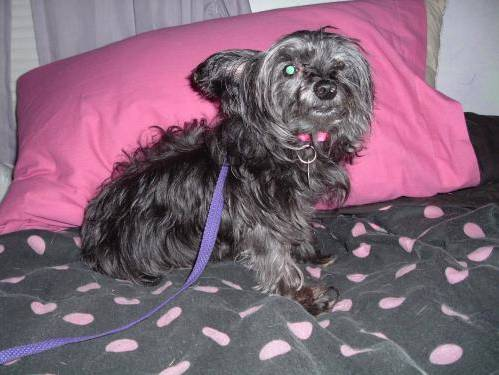
\includegraphics[width=1.2cm]{data/dog.0.jpg}
			};
			\node[anchor=west] (dogtext1) at ($ (dog1.east) + (1.2, 0) $) {Hund};
			\draw[->] (dog1) -- (dogtext1);
			\node[anchor=north] (cat2) at ($ (dog1.south) + (0, -0.1) $) {
				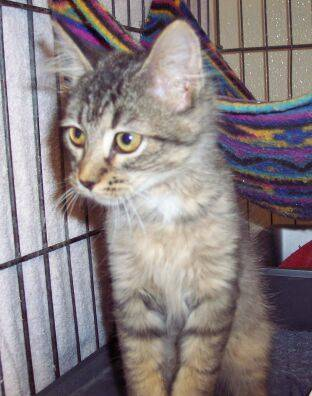
\includegraphics[width=1.2cm]{data/cat.2.jpg}
			};
			\node[anchor=west] (cattext2) at ($ (cat2.east) + (1.2, 0) $) {Katt};
			\draw[->] (cat2) -- (cattext2);
			\node[anchor=north] (dog2) at ($ (cat2.south) + (0, -0.1) $) {
				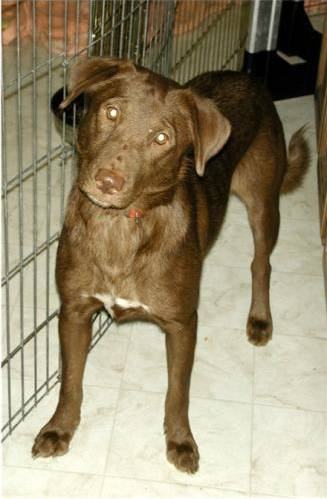
\includegraphics[width=1.2cm]{data/dog.1.jpg}
			};
			\node[anchor=west] (dogtext2) at ($ (dog2.east) + (1.2, 0) $) {Hund};
			\draw[->] (dog2) -- (dogtext2);

			\node[] (cat1) at ($ (unsupervised.south) + (-1.2, -2.4) $) {
				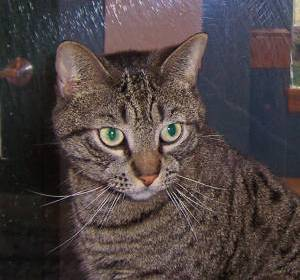
\includegraphics[width=0.8cm]{data/cat.1.jpg}
			};
			\node[] (cat2) at ($ (cat1) + (-0.9, 0.2) $) {
				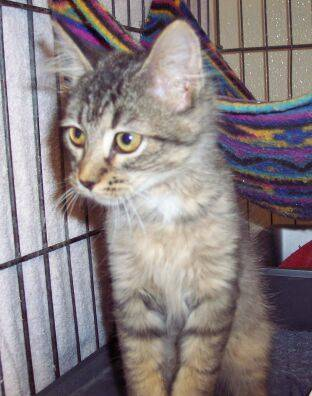
\includegraphics[width=0.8cm]{data/cat.2.jpg}
			};
			\node[] (cat3) at ($ (cat1) + (-0.5, -0.8) $) {
				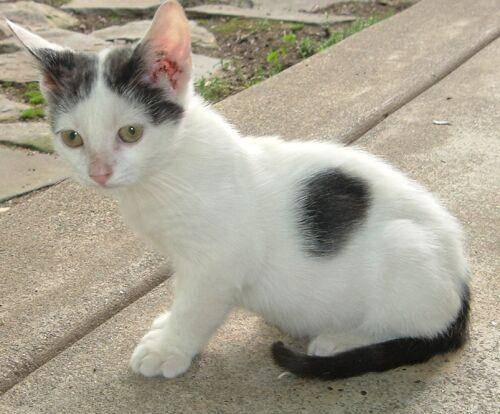
\includegraphics[width=0.8cm]{data/cat.3.jpg}
			};
			\node[] (cat4) at ($ (cat1) + (0.9, -0.1) $) {
				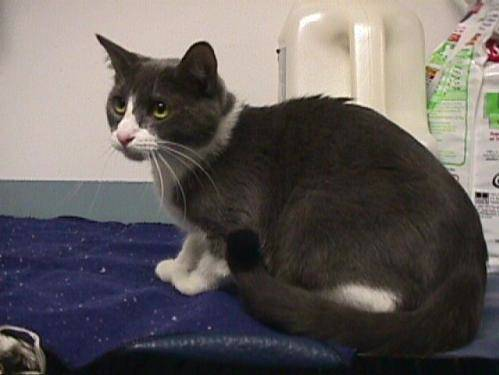
\includegraphics[width=0.8cm]{data/cat.4.jpg}
			};

			\node[] (dog1) at ($ (cat1) + (1.8, -1.5) $) {
				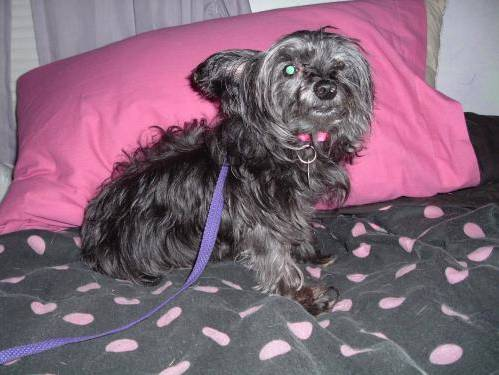
\includegraphics[width=0.8cm]{data/dog.0.jpg}
			};
			\node[] (dog2) at ($ (dog1) + (0.9, 0.1) $) {
				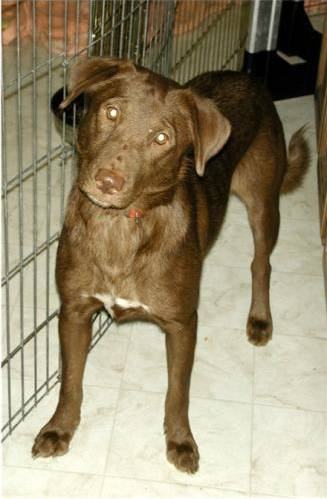
\includegraphics[width=0.8cm]{data/dog.1.jpg}
			};
			\node[] (dog3) at ($ (dog1) + (0.3, -0.8) $) {
				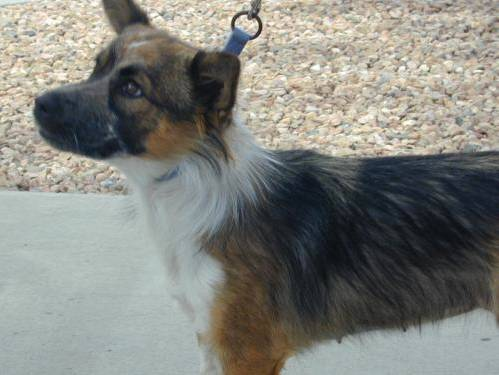
\includegraphics[width=0.8cm]{data/dog.3.jpg}
			};
			\node[] (dog4) at ($ (dog1) + (-0.9, -0.3) $) {
				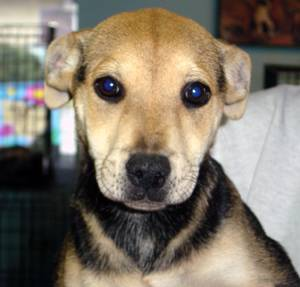
\includegraphics[width=0.8cm]{data/dog.4.jpg}
			};
			\draw[dashed, thick, red] ($ (cat1) + (-0.9, -1.7) $) -- ($ (dog1) + (1.2, 1.7) $);
		\end{tikzpicture}
		\vfill
	\end{frame}

	\begin{frame}{Terminology: Smal og generell AI} % Strong vs weak, axis
		\centering
		\vfill
		\begin{tikzpicture}
			\draw[<->] (0, 0) -- (10, 0);
			\node[anchor=north west] at (0, -0.1) {Mer spesifikk};
			\node[anchor=north east] at (10, -0.1) {Mer generell};
			\node[anchor=north west] at (0, 6) {Smal (svak)};
			\node[anchor=north east] at (10, 6) {Generell (sterk)};

			\draw[red, ->, thick] (2, 4) -- (8, 4);
			\node[anchor=south,align=center,text=red] at (5, 4.1) {I stand til å løse et bredere spekter med\\problemer innenfor flere domener};

			\node[] at (10.2, -0.4) {};
			\node[] at (-0.2, 5.9) {};
		\end{tikzpicture}
		\vfill
	\end{frame}

	\begin{frame}{Terminology: Smal og generell AI} % Strong vs weak, dichotomi
		\centering
		\vfill
		\begin{tikzpicture}
			\draw[<->] (0, 0) -- (10, 0);
			\node[anchor=north west] at (0, -0.1) {Mer spesifikk};
			\node[anchor=north east] at (10, -0.1) {Mer generell};
			\node[anchor=north west] at (0, 6) {Smal (svak)};
			\node[anchor=north east] at (10, 6) {Generell (sterk)};

			\draw[red, ->, thick] (2, 4) -- (8, 4);
			\node[anchor=south,align=center,text=red] at (5, 4.1) {I stand til å løse et bredere spekter med\\problemer innenfor flere domener};
			\node[anchor=south east] at (9.5, 0.2) {
				
\includegraphics[width=1.3cm]{data/human.png}
			};
			\node[anchor=south west] at (0.5, 0.2) {
				
\includegraphics[width=1.3cm]{data/laptop.png}
			};
			\node[] at (10.2, -0.4) {};
			\node[] at (-0.2, 5.9) {};
		\end{tikzpicture}
		\vfill
	\end{frame}

	\begin{frame}{Terminology: Smal og generell AI} % Strong vs weak, weak
		\centering
		\vfill
		\begin{tikzpicture}
			\draw[<->] (0, 0) -- (10, 0);
			\node[anchor=north west] at (0, -0.1) {Mer spesifikk};
			\node[anchor=north east] at (10, -0.1) {Mer generell};
			\node[anchor=north west] at (0, 6) {Smal (svak)};
			\node[anchor=north east] at (10, 6) {Generell (sterk)};

			\draw[red, ->, thick] (2, 4) -- (8, 4);
			\node[anchor=south,align=center,text=red] at (5, 4.1) {I stand til å løse et bredere spekter med\\problemer innenfor flere domener};
			\node[anchor=south east] at (9.5, 0.2) {
				
\includegraphics[width=1.3cm]{data/human.png}
			};
			\node[anchor=south west] at (0.5, 0.2) {
				
\includegraphics[width=1.3cm]{data/laptop.png}
			};
			\node[align=center,font=\small, fill=blue!60, text=white, minimum width=1.6cm, rounded corners=.1cm] at (3, 2.1) {
				Bilde-\\
				diagnostikk
			};
			\node[align=center,font=\small, fill=blue!60, text=white, minimum width=1.6cm, rounded corners=.1cm] at (3, 1.3) {
				Forsikrings-\\
				prising
			};
			\node[align=center,font=\small, fill=blue!60, text=white, minimum width=1.6cm, rounded corners=.1cm] at (3, 0.5) {
				Dokument-\\
				lesing
			};
			\node[] at (10.2, -0.4) {};
			\node[] at (-0.2, 5.9) {};
		\end{tikzpicture}
		\vfill
	\end{frame}

	\begin{frame}{Terminology: Smal og generell AI} % Strong vs weak, stronger
		\centering
		\vfill
		\begin{tikzpicture}
			\draw[<->] (0, 0) -- (10, 0);
			\node[anchor=north west] at (0, -0.1) {Mer spesifikk};
			\node[anchor=north east] at (10, -0.1) {Mer generell};
			\node[anchor=north west] at (0, 6) {Smal (svak)};
			\node[anchor=north east] at (10, 6) {Generell (sterk)};

			\draw[red, ->, thick] (2, 4) -- (8, 4);
			\node[anchor=south,align=center,text=red] at (5, 4.1) {I stand til å løse et bredere spekter med\\problemer innenfor flere domener};
			\node[anchor=south east] at (9.5, 0.2) {
				
\includegraphics[width=1.3cm]{data/human.png}
			};
			\node[anchor=south west] at (0.5, 0.2) {
				
\includegraphics[width=1.3cm]{data/laptop.png}
			};
			\node[align=center,font=\small, fill=blue!60, text=white, minimum width=1.6cm, rounded corners=.1cm] at (3, 2.1) {
				Bilde-\\
				diagnostikk
			};
			\node[align=center,font=\small, fill=blue!60, text=white, minimum width=1.6cm, rounded corners=.1cm] at (3, 1.3) {
				Forsikrings-\\
				prising
			};
			\node[align=center,font=\small, fill=blue!60, text=white, minimum width=1.6cm, rounded corners=.1cm] at (3, 0.5) {
				Dokument-\\
				lesing
			};
			\node[align=center,font=\small, fill=blue!60, text=white, minimum width=1.6cm, rounded corners=.1cm] at (4.8, 0.5) {
				Tesla
			};
			\node[align=center,font=\small, fill=blue!60, text=white, minimum width=1.6cm, rounded corners=.1cm] at (5.4, 1.1) {
				ChatGPT
			};
			\node[] at (10.2, -0.4) {};
			\node[] at (-0.2, 5.9) {};
		\end{tikzpicture}
		\vfill
	\end{frame}

	\section{Teori}

	\begin{frame}{Teori: Maskinlæringsmodeller}
		\centering
		\begin{tikzpicture}
			\node[minimum width=2.5cm, minimum height=1.5cm, draw=black, fill=gray!10] (model) at (0, 0) {Modell};
			\node[anchor=east] (in) at (-3, 0) {Input};
			\node[anchor=west] (out) at (3, 0) {Output};

			\draw[->] (in) -- (model);
			\draw[->] (model) -- (out);

			\node[] at (-4, 2) {};
			\node[] at (4, -2) {};

		\end{tikzpicture}
	\end{frame}

	\begin{frame}{Teori: Maskinlæringsmodeller}
		\centering
		\begin{tikzpicture}
			\node[minimum width=2.5cm, minimum height=1.5cm, draw=black, fill=gray!10] (model) at (0, 0) {Modell};
			\node[anchor=east] (in) at (-3, 0) {Areal};
			\node[anchor=west] (out) at (3, 0) {Pris};

			\draw[->] (in) -- (model);
			\draw[->] (model) -- (out);

			\node[] at (-4, 2) {};
			\node[] at (4, -2) {};

		\end{tikzpicture}
	\end{frame}

	\begin{frame}{Teori: Maskinlæringsmodeller} % Finn.no data
		\centering
		\vfill
		\begin{tikzpicture}
			\node[draw=black, inner sep=0pt] at (0, 0) {
				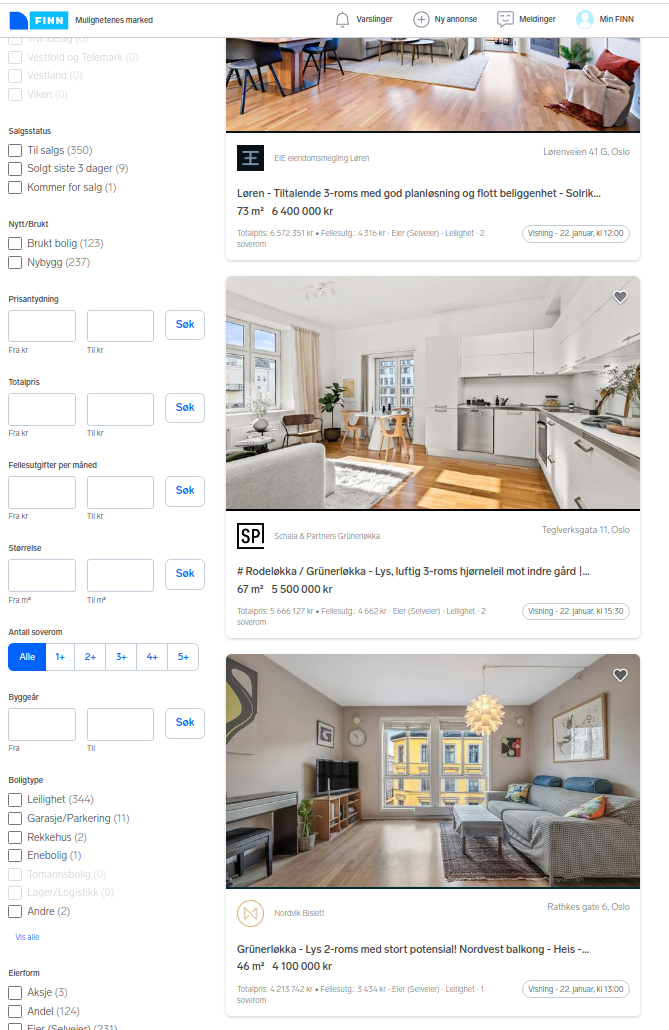
\includegraphics[height=7cm]{data/finn.png}
			};
		\end{tikzpicture}
		\vfill
	\end{frame}

	\colorlet{model1}{red}
	\colorlet{model2}{green}
	\colorlet{model3}{orange}

	\begin{frame}{Teori: Maskinlæringsmodeller} % Dataset
		\centering
		\vfill
		\begin{table}
			\begin{tabular}{|c|c|}
				\hline
				\textbf{$m^2$}&\textbf{Pris}\\
				\hline
				72&5.127.379\\
				\hline
				50&4.552.170\\
				\hline
				45&4.486.654\\
				\hline
				62&5.709.276\\
				\hline
				53&4.634.912\\
				\hline
				81&8.388.570\\
				\hline
				44&4.828.170\\
				\hline
				78&7.557.770\\
				\hline
				37&4.016.520\\
				\hline
				73&6.572.351\\
				\hline
			\end{tabular}
		\end{table}
		\vfill
	\end{frame}

	\begin{frame}{Teori: Maskinlæringsmodeller} % 2d dataset
		\vfill
		\begin{tikzpicture}
			\begin{axis}[
				xlabel=$m^2$,
				ylabel=NOK,
				ytick={4000000, 5000000, 6000000, 7000000, 8000000},
				yticklabels={4M, 5M, 6M, 7M, 8M},
				scaled y ticks=false,
				xtick pos=bottom,
				ytick pos=left,
				xmin=30,
				xmax=90,,
				ymin=3500000,
				ymax=8800000
			]
				\addplot[
					only marks,
					mark size=3pt,
					mark options={draw=black, fill=cyan}
				] coordinates {
					(72, 5127379)
					(50, 4552170)
					(45, 4486654)
					(62, 5709276)
					(53, 4634912)
					(81, 8388570)
					(44, 4828170)
					(78, 7557770)
					(37, 4016520)
					(73, 6572351)
				};

				\newcommand{\loss}[2]{
					\addplot[dashed] coordinates {
						(####1, 3500000 + ####1 * 30000)
						(####1, ####2)
					};
				}

				\coordinate (center) at (axis cs: 60, 3500000);
			\end{axis}

			\node[] at ($ (center) - (5.3, 1.8) $) {};
			\node[] at ($ (center) + (5.3, 5.8) $) {};
		\end{tikzpicture}
		\vfill
	\end{frame}

	\begin{frame}{Teori: Maskinlæringsmodeller} % Use case
		\vfill
		\begin{tikzpicture}
			\begin{axis}[
				xlabel=$m^2$,
				ylabel=NOK,
				ytick={4000000, 5000000, 6000000, 7000000, 8000000},
				yticklabels={4M, 5M, 6M, 7M, 8M},
				scaled y ticks=false,
				xtick pos=bottom,
				ytick pos=left,
				xmin=30,
				xmax=90,,
				ymin=3500000,
				ymax=8800000
			]
				\addplot[
					only marks,
					mark size=3pt,
					mark options={draw=black, fill=cyan}
				] coordinates {
					(72, 5127379)
					(50, 4552170)
					(45, 4486654)
					(62, 5709276)
					(53, 4634912)
					(81, 8388570)
					(44, 4828170)
					(78, 7557770)
					(37, 4016520)
					(73, 6572351)
				};
				\addplot[red, thick] coordinates {
					(57, 3500000)
					(57, 8800000)
				};

				\coordinate (center) at (axis cs: 60, 3500000);
			\end{axis}
			\node[anchor=north,align=center] (m1) at ($ (center) - (0, 1) $) {
				$\hat{y}=f($\textcolor{red}{$57$}$)$
			};

			\node[] at ($ (center) - (5.3, 1.8) $) {};
			\node[] at ($ (center) + (5.3, 5.8) $) {};
		\end{tikzpicture}
		\vfill
	\end{frame}

	\begin{frame}{Teori: Maskinlæringsmodeller} % Concrete model
		\vfill
		\begin{tikzpicture}
			\begin{axis}[
				xlabel=$m^2$,
				ylabel=NOK,
				ytick={4000000, 5000000, 6000000, 7000000, 8000000},
				yticklabels={4M, 5M, 6M, 7M, 8M},
				scaled y ticks=false,
				xtick pos=bottom,
				ytick pos=left,
				xmin=30,
				xmax=90,,
				ymin=3500000,
				ymax=8800000
			]
				\addplot[
					only marks,
					mark size=3pt,
					mark options={draw=black, fill=cyan}
				] coordinates {
					(72, 5127379)
					(50, 4552170)
					(45, 4486654)
					(62, 5709276)
					(53, 4634912)
					(81, 8388570)
					(44, 4828170)
					(78, 7557770)
					(37, 4016520)
					(73, 6572351)
				};
				\addplot[model2] coordinates {
					(0, 3500000)
					(100, 6500000)
				};

				\newcommand{\loss}[2]{
					\addplot[dashed] coordinates {
						(####1, 3500000 + ####1 * 30000)
						(####1, ####2)
					};
				}

				\coordinate (center) at (axis cs: 60, 3500000);
			\end{axis}

			\node[] at ($ (center) - (5.3, 1.8) $) {};
			\node[] at ($ (center) + (5.3, 5.8) $) {};
		\end{tikzpicture}
		\vfill
	\end{frame}

	\begin{frame}{Teori: Maskinlæringsmodeller} % Concrete model
		\vfill
		\begin{tikzpicture}
			\begin{axis}[
				xlabel=$m^2$,
				ylabel=NOK,
				ytick={4000000, 5000000, 6000000, 7000000, 8000000},
				yticklabels={4M, 5M, 6M, 7M, 8M},
				scaled y ticks=false,
				xtick pos=bottom,
				ytick pos=left,
				xmin=30,
				xmax=90,,
				ymin=3500000,
				ymax=8800000
			]
				\addplot[
					only marks,
					mark size=3pt,
					mark options={draw=black, fill=cyan}
				] coordinates {
					(72, 5127379)
					(50, 4552170)
					(45, 4486654)
					(62, 5709276)
					(53, 4634912)
					(81, 8388570)
					(44, 4828170)
					(78, 7557770)
					(37, 4016520)
					(73, 6572351)
				};
				\addplot[model2] coordinates {
					(0, 3500000)
					(100, 6500000)
				};

				\newcommand{\loss}[2]{
					\addplot[dashed] coordinates {
						(####1, 3500000 + ####1 * 30000)
						(####1, ####2)
					};
				}

				\coordinate (center) at (axis cs: 60, 3500000);
			\end{axis}
			\node[anchor=north,align=center, text=model2] (m1) at ($ (center) - (0, 1) $) {
				$\hat{y}=30000x + 3500000$
			};

			\node[] at ($ (center) - (5.3, 1.8) $) {};
			\node[] at ($ (center) + (5.3, 5.8) $) {};
		\end{tikzpicture}
		\vfill
	\end{frame}

	\begin{frame}{Teori: Maskinlæringsmodeller} % Alternative models
		\vfill
		\begin{tikzpicture}
			\begin{axis}[
				xlabel=$m^2$,
				ylabel=NOK,
				ytick={4000000, 5000000, 6000000, 7000000, 8000000},
				yticklabels={4M, 5M, 6M, 7M, 8M},
				scaled y ticks=false,
				xtick pos=bottom,
				ytick pos=left,
				xmin=30,
				xmax=90,,
				ymin=3500000,
				ymax=8800000
			]
				\addplot[
					only marks,
					mark size=3pt,
					mark options={draw=black, fill=cyan}
				] coordinates {
					(72, 5127379)
					(50, 4552170)
					(45, 4486654)
					(62, 5709276)
					(53, 4634912)
					(81, 8388570)
					(44, 4828170)
					(78, 7557770)
					(37, 4016520)
					(73, 6572351)
				};
				\addplot[model1] coordinates {
					(0, 6000000)
					(100, 6000000)
				};
				\addplot[model2] coordinates {
					(0, 3500000)
					(100, 6500000)
				};
				\addplot[model3] coordinates {
					(0, 706495)
					(100, 8909658)
				};

				\newcommand{\loss}[2]{
					\addplot[dashed] coordinates {
						(####1, 3500000 + ####1 * 30000)
						(####1, ####2)
					};
				}

				\coordinate (center) at (axis cs: 60, 3500000);
			\end{axis}
			\node[anchor=north,align=center, text=model2] (m1) at ($ (center) - (0, 1) $) {
				$\hat{y}=30000x + 3500000$
			};

			\node[anchor=east,align=center, text=model1] at ($ (m1.west) + (-1, 0) $) {
				$\hat{y}=0x + 6000000$
			};

			\node[anchor=west,align=center, text=model3] at ($ (m1.east) + (1, 0) $) {
				$\hat{y}=82031x + 706495$
			};

			\node[] at ($ (center) - (5.3, 1.8) $) {};
			\node[] at ($ (center) + (5.3, 5.8) $) {};
		\end{tikzpicture}
		\vfill
	\end{frame}

	\begin{frame}{Teori: Kostfunksjon} % Model
		\vfill
		\begin{tikzpicture}
			\begin{axis}[
				xlabel=$m^2$,
				ylabel=NOK,
				ytick={4000000, 5000000, 6000000, 7000000, 8000000},
				yticklabels={4M, 5M, 6M, 7M, 8M},
				scaled y ticks=false,
				xtick pos=bottom,
				ytick pos=left,
				xmin=30,
				xmax=90,,
				ymin=3500000,
				ymax=8800000
			]
				\addplot[
					only marks,
					mark size=3pt,
					mark options={draw=black, fill=cyan}
				] coordinates {
					(72, 5127379)
					(50, 4552170)
					(45, 4486654)
					(62, 5709276)
					(53, 4634912)
					(81, 8388570)
					(44, 4828170)
					(78, 7557770)
					(37, 4016520)
					(73, 6572351)
				};
				\addplot[model2] coordinates {
					(0, 3500000)
					(100, 6500000)
				};

				\newcommand{\loss}[2]{
					\addplot[dashed] coordinates {
						(####1, 3500000 + ####1 * 30000)
						(####1, ####2)
					};
				}

				\coordinate (center) at (axis cs: 60, 3500000);
			\end{axis}
			\node[anchor=north,align=center, text=model2] (m1) at ($ (center) - (0, 1) $) {
				$\hat{y}=30000x + 3500000$
			};

			\node[] at ($ (center) - (5.3, 1.8) $) {};
			\node[] at ($ (center) + (5.3, 5.8) $) {};
		\end{tikzpicture}
		\vfill
	\end{frame}

	\begin{frame}{Teori: Kostfunksjon} % Prediction
		\vfill
		\begin{tikzpicture}
			\begin{axis}[
				xlabel=$m^2$,
				ylabel=NOK,
				ytick={4000000, 5000000, 6000000, 7000000, 8000000},
				yticklabels={4M, 5M, 6M, 7M, 8M},
				scaled y ticks=false,
				xtick pos=bottom,
				ytick pos=left,
				xmin=30,
				xmax=90,,
				ymin=3500000,
				ymax=8800000
			]
				\addplot[
					only marks,
					mark size=3pt,
					mark options={draw=black, fill=cyan}
				] coordinates {
					(72, 5127379)
					(50, 4552170)
					(45, 4486654)
					(62, 5709276)
					(53, 4634912)
					(81, 8388570)
					(44, 4828170)
					(78, 7557770)
					(37, 4016520)
					(73, 6572351)
				};
				\addplot[
					only marks,
					mark size=3pt,
					mark options={draw=green, fill=white},
					fill opacity=0
				] coordinates {
					(78, 3500000 + 78 * 30000)
				};
				\addplot[model2] coordinates {
					(0, 3500000)
					(100, 6500000)
				};

				\newcommand{\loss}[2]{
					\addplot[dashed] coordinates {
						(####1, 3500000 + ####1 * 30000)
						(####1, ####2)
					};
				}

				\coordinate (center) at (axis cs: 60, 3500000);
				\node[anchor=west] at (axis cs: 79, 5840000) {\footnotesize{$\hat{y}$}};
				\node[anchor=west] at (axis cs: 79, 7557770) {\footnotesize{$y$}};
			\end{axis}
			\node[anchor=north,align=center, text=model2] (m1) at ($ (center) - (0, 1) $) {
				$\hat{y}=30000x + 3500000$
			};

			\node[] at ($ (center) - (5.3, 1.8) $) {};
			\node[] at ($ (center) + (5.3, 5.8) $) {};
		\end{tikzpicture}
		\vfill
	\end{frame}

	\begin{frame}{Teori: Kostfunksjon} % Squared error
		\vfill
		\begin{tikzpicture}
			\begin{axis}[
				xlabel=$m^2$,
				ylabel=NOK,
				ytick={4000000, 5000000, 6000000, 7000000, 8000000},
				yticklabels={4M, 5M, 6M, 7M, 8M},
				scaled y ticks=false,
				xtick pos=bottom,
				ytick pos=left,
				xmin=30,
				xmax=90,,
				ymin=3500000,
				ymax=8800000
			]
				\addplot[
					only marks,
					mark size=3pt,
					mark options={draw=black, fill=cyan}
				] coordinates {
					(72, 5127379)
					(50, 4552170)
					(45, 4486654)
					(62, 5709276)
					(53, 4634912)
					(81, 8388570)
					(44, 4828170)
					(78, 7557770)
					(37, 4016520)
					(73, 6572351)
				};
				\addplot[
					only marks,
					mark size=3pt,
					mark options={draw=green, fill=white},
					fill opacity=0
				] coordinates {
					(78, 3500000 + 78 * 30000)
				};
				\addplot[model2] coordinates {
					(0, 3500000)
					(100, 6500000)
				};

				\newcommand{\loss}[2]{
					\addplot[dashed] coordinates {
						(####1, 3500000 + ####1 * 30000)
						(####1, ####2)
					};
				}

				\loss{78}{7557770}

				\coordinate (center) at (axis cs: 60, 3500000);
				\node[anchor=west] at (axis cs: 79, 5840000) {\footnotesize{$\hat{y}$}};
				\node[anchor=west] at (axis cs: 79, 7557770) {\footnotesize{$y$}};
				\node[anchor=west] at (axis cs: 78, 6698885) {\footnotesize{$\ell=(y-\hat{y})^2$}};
			\end{axis}
			\node[anchor=north,align=center, text=model2] (m1) at ($ (center) - (0, 1) $) {
				$\hat{y}=30000x + 3500000$
			};

			\node[] at ($ (center) - (5.3, 1.8) $) {};
			\node[] at ($ (center) + (5.3, 5.8) $) {};
		\end{tikzpicture}
		\vfill
	\end{frame}

	\begin{frame}{Teori: Kostfunksjon} % Mean squared error
		\vfill
		\begin{tikzpicture}
			\begin{axis}[
				xlabel=$m^2$,
				ylabel=NOK,
				ytick={4000000, 5000000, 6000000, 7000000, 8000000},
				yticklabels={4M, 5M, 6M, 7M, 8M},
				scaled y ticks=false,
				xtick pos=bottom,
				ytick pos=left,
				xmin=30,
				xmax=90,,
				ymin=3500000,
				ymax=8800000
			]
				\addplot[
					only marks,
					mark size=3pt,
					mark options={draw=black, fill=cyan}
				] coordinates {
					(72, 5127379)
					(50, 4552170)
					(45, 4486654)
					(62, 5709276)
					(53, 4634912)
					(81, 8388570)
					(44, 4828170)
					(78, 7557770)
					(37, 4016520)
					(73, 6572351)
				};
				\addplot[
					only marks,
					mark size=3pt,
					mark options={draw=green, fill=white},
					fill opacity=0
				] coordinates {
					(72, 3500000 + 72 * 30000)
					(50, 3500000 + 50 * 30000)
					(45, 3500000 + 45 * 30000)
					(62, 3500000 + 62 * 30000)
					(53, 3500000 + 53 * 30000)
					(81, 3500000 + 81 * 30000)
					(44, 3500000 + 44 * 30000)
					(78, 3500000 + 78 * 30000)
					(37, 3500000 + 37 * 30000)
					(73, 3500000 + 73 * 30000)
				};
				\addplot[model2] coordinates {
					(0, 3500000)
					(100, 6500000)
				};

				\newcommand{\loss}[2]{
					\addplot[dashed] coordinates {
						(####1, 3500000 + ####1 * 30000)
						(####1, ####2)
					};
				}

				\loss{72}{5127379}
				\loss{50}{4552170}
				\loss{45}{4486654}
				\loss{62}{5709276}
				\loss{53}{4634912}
				\loss{81}{8388570}
				\loss{44}{4828170}
				\loss{78}{7557770}
				\loss{37}{4016520}
				\loss{73}{6572351}

				\coordinate (center) at (axis cs: 60, 3500000);
			\end{axis}
			\node[anchor=north,align=center, text=model2] (m1) at ($ (center) - (0, 1) $) {
				$\hat{y}=30000x + 3500000$\\
				$\ell=\sum (y - \hat{y})^2$
			};

			\node[] at ($ (center) - (5.3, 1.8) $) {};
			\node[] at ($ (center) + (5.3, 5.8) $) {};
		\end{tikzpicture}
		\vfill
	\end{frame}

	\begin{frame}{Teori: Kostfunksjon} % Loss computation
		\vfill
		\begin{tikzpicture}
			\begin{axis}[
				xlabel=$m^2$,
				ylabel=NOK,
				ytick={4000000, 5000000, 6000000, 7000000, 8000000},
				yticklabels={4M, 5M, 6M, 7M, 8M},
				scaled y ticks=false,
				xtick pos=bottom,
				ytick pos=left,
				xmin=30,
				xmax=90,,
				ymin=3500000,
				ymax=8800000
			]
				\addplot[
					only marks,
					mark size=3pt,
					mark options={draw=black, fill=cyan}
				] coordinates {
					(72, 5127379)
					(50, 4552170)
					(45, 4486654)
					(62, 5709276)
					(53, 4634912)
					(81, 8388570)
					(44, 4828170)
					(78, 7557770)
					(37, 4016520)
					(73, 6572351)
				};
				\addplot[
					only marks,
					mark size=3pt,
					mark options={draw=green, fill=white},
					fill opacity=0
				] coordinates {
					(72, 3500000 + 72 * 30000)
					(50, 3500000 + 50 * 30000)
					(45, 3500000 + 45 * 30000)
					(62, 3500000 + 62 * 30000)
					(53, 3500000 + 53 * 30000)
					(81, 3500000 + 81 * 30000)
					(44, 3500000 + 44 * 30000)
					(78, 3500000 + 78 * 30000)
					(37, 3500000 + 37 * 30000)
					(73, 3500000 + 73 * 30000)
				};
				\addplot[model2] coordinates {
					(0, 3500000)
					(100, 6500000)
				};

				\newcommand{\loss}[2]{
					\addplot[dashed] coordinates {
						(####1, 3500000 + ####1 * 30000)
						(####1, ####2)
					};
				}

				\loss{72}{5127379}
				\loss{50}{4552170}
				\loss{45}{4486654}
				\loss{62}{5709276}
				\loss{53}{4634912}
				\loss{81}{8388570}
				\loss{44}{4828170}
				\loss{78}{7557770}
				\loss{37}{4016520}
				\loss{73}{6572351}

				\coordinate (center) at (axis cs: 60, 3500000);
			\end{axis}
			\node[anchor=north,align=center, text=model2] (m1) at ($ (center) - (0, 1) $) {
				$\hat{y}=30000x + 3500000$\\
				$\ell=1.10 \times 10^{13}$
			};

			\node[] at ($ (center) - (5.3, 1.8) $) {};
			\node[] at ($ (center) + (5.3, 5.8) $) {};
		\end{tikzpicture}
		\vfill
	\end{frame}

	\begin{frame}{Teori: Kostfunksjon} % Loss comparison
		\vfill
		\begin{tikzpicture}
			\begin{axis}[
				xlabel=$m^2$,
				ylabel=NOK,
				ytick={4000000, 5000000, 6000000, 7000000, 8000000},
				yticklabels={4M, 5M, 6M, 7M, 8M},
				scaled y ticks=false,
				xtick pos=bottom,
				ytick pos=left,
				xmin=30,
				xmax=90,,
				ymin=3500000,
				ymax=8800000
			]
				\addplot[
					only marks,
					mark size=3pt,
					mark options={draw=black, fill=cyan}
				] coordinates {
					(72, 5127379)
					(50, 4552170)
					(45, 4486654)
					(62, 5709276)
					(53, 4634912)
					(81, 8388570)
					(44, 4828170)
					(78, 7557770)
					(37, 4016520)
					(73, 6572351)
				};
				\addplot[model1] coordinates {
					(0, 6000000)
					(100, 6000000)
				};
				\addplot[model2] coordinates {
					(0, 3500000)
					(100, 6500000)
				};
				\addplot[model3] coordinates {
					(0, 706495)
					(100, 8909658)
				};
				\coordinate (center) at (axis cs: 60, 3500000);
			\end{axis}
			\node[anchor=north,align=center, text=model2] (m1) at ($ (center) - (0, 1) $) {
				$\hat{y}=30000x + 3500000$\\
				$\ell=1.10 \times 10^{13}$
			};


			\node[anchor=east,align=center, text=model1] at ($ (m1.west) + (-1, 0) $) {
				$\hat{y}=0x + 6000000$\\
				$\ell=2.08 \times 10^{13}$
			};

			\node[anchor=west,align=center, text=model3] at ($ (m1.east) + (1, 0) $) {
				$\hat{y}=82031x + 706495$\\
				$\ell=4.09 \times 10^{12}$
			};

			\node[] at ($ (center) - (5.3, 1.8) $) {};
			\node[] at ($ (center) + (5.3, 5.8) $) {};
		\end{tikzpicture}
		\vfill
	\end{frame}

	\begin{frame}{Teori: Trening} % Formulas
		\vfill
		\begin{tikzpicture}
			\begin{axis}[
				xlabel=$m^2$,
				ylabel=NOK,
				ytick={4000000, 5000000, 6000000, 7000000, 8000000},
				yticklabels={4M, 5M, 6M, 7M, 8M},
				scaled y ticks=false,
				xtick pos=bottom,
				ytick pos=left,
				xmin=30,
				xmax=90,,
				ymin=3500000,
				ymax=8800000
			]
				\addplot[
					only marks,
					mark size=3pt,
					mark options={draw=black, fill=cyan}
				] coordinates {
					(72, 5127379)
					(50, 4552170)
					(45, 4486654)
					(62, 5709276)
					(53, 4634912)
					(81, 8388570)
					(44, 4828170)
					(78, 7557770)
					(37, 4016520)
					(73, 6572351)
				};
				\addplot[model2] coordinates {
					(0, 3500000)
					(100, 6500000)
				};
				\coordinate (center) at (axis cs: 60, 3500000);
			\end{axis}
			\node[anchor=north,align=center] (m1) at ($ (center) - (0, 1) $) {
				$\hat{y}=wx + b$\\
				$\ell=\sum (y - \hat{y})^2$
			};

			\node[] at ($ (center) - (5.3, 1.8) $) {};
			\node[] at ($ (center) + (5.3, 5.8) $) {};
		\end{tikzpicture}
		\vfill
	\end{frame}

	\begin{frame}{Teori: Trening} % Formula replacement
		\vfill
		\begin{tikzpicture}
			\begin{axis}[
				xlabel=$m^2$,
				ylabel=NOK,
				ytick={4000000, 5000000, 6000000, 7000000, 8000000},
				yticklabels={4M, 5M, 6M, 7M, 8M},
				scaled y ticks=false,
				xtick pos=bottom,
				ytick pos=left,
				xmin=30,
				xmax=90,,
				ymin=3500000,
				ymax=8800000
			]
				\addplot[
					only marks,
					mark size=3pt,
					mark options={draw=black, fill=cyan}
				] coordinates {
					(72, 5127379)
					(50, 4552170)
					(45, 4486654)
					(62, 5709276)
					(53, 4634912)
					(81, 8388570)
					(44, 4828170)
					(78, 7557770)
					(37, 4016520)
					(73, 6572351)
				};
				\addplot[model2] coordinates {
					(0, 3500000)
					(100, 6500000)
				};
				\coordinate (center) at (axis cs: 60, 3500000);
			\end{axis}


			\node[anchor=north,align=center] (m1) at ($ (center) - (0, 1) $) {
				$\hat{y}=wx + b$\\
				$\ell=\sum (y - \hat{y})^2$
			};
			\node[
				draw=red,
				anchor=north west,
				minimum height=0.4cm,
				minimum width=0.3cm
			] at ($ (m1.north west) + (0.21, -0.03) $) {};
			\node[
				draw=red,
				anchor=south east,
				minimum height=0.4cm,
				minimum width=0.3cm
			] at ($ (m1.south east) + (-0.27, 0.05) $) {};

			\node[] at ($ (center) - (5.3, 1.8) $) {};
			\node[] at ($ (center) + (5.3, 5.8) $) {};
		\end{tikzpicture}
		\vfill
	\end{frame}

	\begin{frame}{Teori: Trening} % Single formula
		\vfill
		\begin{tikzpicture}
			\begin{axis}[
				xlabel=$m^2$,
				ylabel=NOK,
				ytick={4000000, 5000000, 6000000, 7000000, 8000000},
				yticklabels={4M, 5M, 6M, 7M, 8M},
				scaled y ticks=false,
				xtick pos=bottom,
				ytick pos=left,
				xmin=30,
				xmax=90,,
				ymin=3500000,
				ymax=8800000
			]
				\addplot[
					only marks,
					mark size=3pt,
					mark options={draw=black, fill=cyan}
				] coordinates {
					(72, 5127379)
					(50, 4552170)
					(45, 4486654)
					(62, 5709276)
					(53, 4634912)
					(81, 8388570)
					(44, 4828170)
					(78, 7557770)
					(37, 4016520)
					(73, 6572351)
				};
				\addplot[model2] coordinates {
					(0, 3500000)
					(100, 6500000)
				};
				\coordinate (center) at (axis cs: 60, 3500000);
			\end{axis}


			\node[anchor=north,align=center] (m1) at ($ (center) - (0, 1) $) {
				$\ell=\sum (y - (wx + b))^2$
			};

			\node[] at ($ (center) - (5.3, 1.8) $) {};
			\node[] at ($ (center) + (5.3, 5.8) $) {};
		\end{tikzpicture}
		\vfill
	\end{frame}

	\begin{frame}{Teori: Trening} % Actual formula
		\vfill
		\begin{tikzpicture}
			\begin{axis}[
				xlabel=$m^2$,
				ylabel=NOK,
				ytick={4000000, 5000000, 6000000, 7000000, 8000000},
				yticklabels={4M, 5M, 6M, 7M, 8M},
				scaled y ticks=false,
				xtick pos=bottom,
				ytick pos=left,
				xmin=30,
				xmax=90,,
				ymin=3500000,
				ymax=8800000
			]
				\addplot[
					only marks,
					mark size=3pt,
					mark options={draw=black, fill=cyan}
				] coordinates {
					(72, 5127379)
					(50, 4552170)
					(45, 4486654)
					(62, 5709276)
					(53, 4634912)
					(81, 8388570)
					(44, 4828170)
					(78, 7557770)
					(37, 4016520)
					(73, 6572351)
				};
				\addplot[model2] coordinates {
					(0, 3500000)
					(100, 6500000)
				};
				\coordinate (center) at (axis cs: 60, 3500000);
			\end{axis}


			\node[anchor=north,align=center] (m1) at ($ (center) - (0, 1) $) {
				$1.10 \times 10^{13}=\sum (y - (30000x + 3500000))^2$
			};

			\node[] at ($ (center) - (5.3, 1.8) $) {};
			\node[] at ($ (center) + (5.3, 5.8) $) {};
		\end{tikzpicture}
		\vfill
	\end{frame}

	\begin{frame}{Teori: Trening} % Update
		\vfill
		\begin{tikzpicture}
			\begin{axis}[
				xlabel=$m^2$,
				ylabel=NOK,
				ytick={4000000, 5000000, 6000000, 7000000, 8000000},
				yticklabels={4M, 5M, 6M, 7M, 8M},
				scaled y ticks=false,
				xtick pos=bottom,
				ytick pos=left,
				xmin=30,
				xmax=90,,
				ymin=3500000,
				ymax=8800000
			]
				\addplot[
					only marks,
					mark size=3pt,
					mark options={draw=black, fill=cyan}
				] coordinates {
					(72, 5127379)
					(50, 4552170)
					(45, 4486654)
					(62, 5709276)
					(53, 4634912)
					(81, 8388570)
					(44, 4828170)
					(78, 7557770)
					(37, 4016520)
					(73, 6572351)
				};
				\addplot[model2] coordinates {
					(0, 3000000)
					(100, 7500000)
				};
				\coordinate (center) at (axis cs: 60, 3500000);
			\end{axis}


			\node[anchor=north,align=center] (m1) at ($ (center) - (0, 1) $) {
				$7.24 \times 10^{12}=\sum (y - (45000x + 3000000))^2$
			};

			\node[] at ($ (center) - (5.3, 1.8) $) {};
			\node[] at ($ (center) + (5.3, 5.8) $) {};
		\end{tikzpicture}
		\vfill
	\end{frame}

	\begin{frame}{Teori: Trening} % Update
		\centering
		Demo!
	\end{frame}

	\colorlet{nodefill}{green!20}

	\begin{frame}{Teori: Nevrale nettverk} % Linear regression
		\def\nodesize{14pt}
		\centering
		\vfill
		\begin{tikzpicture}
			\node[] at (-5, 3) {};
			\node[] at (5, -4.5) {};

			\node[
				circle,
				draw=black,
				fill=nodefill,
				minimum size=\nodesize,
				inner sep=0pt
			] (n) at (0, 1.5) {};
			\node[] (x) at (-1.5, 1.5) {$x$};
			\node[] (b) at (0, 2.5) {$b$};
			\node[] (y) at (1.5, 1.5) {$\hat{y}$};
			\node[] at (0, 0) {$\hat{y}=wx+b$};

			\draw[->] (x) -- (n) node [midway, above] {$w$};
			\draw[->] (b) -- (n);
			\draw[->] (n) -- (y);
		\end{tikzpicture}
		\vfill
	\end{frame}


	\begin{frame}{Teori: Nevrale nettverk} % 2-layer MLP
		\def\nodesize{14pt}
		\centering
		\vfill
		\begin{tikzpicture}
			\node[] at (-3.5, 1.25) {};
			\node[] at (3.5, -6.25) {};
			\node[
				circle,
				draw=black,
				fill=green!20,
				minimum size=\nodesize,
				inner sep=0pt,
				text depth=0
			] (x0) at (-3, 0.5) {\footnotesize{$x_0$}};
			\node[
				circle,
				draw=black,
				fill=green!20,
				minimum size=\nodesize,
				inner sep=0pt,
				text depth=0
			] (x1) at (-3, -0.5) {\footnotesize{$x_1$}};

			\node[
				circle,
				draw=black,
				fill=green!20,
				minimum size=\nodesize,
				inner sep=0pt
			] (n00) at (-1, 1) {};
			\node[
				circle,
				draw=black,
				fill=green!20,
				minimum size=\nodesize,
				inner sep=0pt
			] (n01) at (-1, 0) {};
			\node[
				circle,
				draw=black,
				fill=green!20,
				minimum size=\nodesize,
				inner sep=0pt
			] (n02) at (-1, -1) {};

			\node[
				circle,
				draw=black,
				fill=green!20,
				minimum size=\nodesize,
				inner sep=0pt
			] (n10) at (1, 1) {};

			\node[
				circle,
				draw=black,
				fill=green!20,
				minimum size=\nodesize,
				inner sep=0pt
			] (n11) at (1, 0) {};
			\node[
				circle,
				draw=black,
				fill=green!20,
				minimum size=\nodesize,
				inner sep=0pt
			] (n12) at (1, -1) {};

			\node[
				circle,
				draw=black,
				fill=green!20,
				minimum size=\nodesize,
				inner sep=0pt,
				text depth=0
			] (y) at (3, 0) {\footnotesize{$\hat{y}$}};

			\draw[->] (x0) -- (n00);
			\draw[->] (x0) -- (n01);
			\draw[->] (x0) -- (n02);
			\draw[->] (x1) -- (n00);
			\draw[->] (x1) -- (n01);
			\draw[->] (x1) -- (n02);

			\draw[->] (n00) -- (n10);
			\draw[->] (n00) -- (n11);
			\draw[->] (n00) -- (n12);
			\draw[->] (n01) -- (n10);
			\draw[->] (n01) -- (n11);
			\draw[->] (n01) -- (n12);
			\draw[->] (n02) -- (n10);
			\draw[->] (n02) -- (n11);
			\draw[->] (n02) -- (n12);

			\draw[->] (n10) -- (y);
			\draw[->] (n11) -- (y);
			\draw[->] (n12) -- (y);

			\def\spacing{-0.1cm}
			\node[anchor=north] at (0, -1.5) {\tiny{
				\begin{math}
					\begin{alignedat}{5}
						\hat{y} &= max(0, &&w^2_{0,0}*max(0, &&w^1_{0,0}*max(0, w^0_{0,0}*x_0+w^0_{1,0}*x_{1}+b_{0,0})+\\[\spacing]
						& && &&w^1_{1,0}*max(0, w^0_{0,1}*x_0+w^0_{1,1}*x_{1}+b_{0,1})+\\[\spacing]
						& && &&w^1_{2,0}*max(0, w^0_{0,2}*x_0+w^0_{1,2}*x_{1}+b_{0,2})+\\[\spacing]
						& && &&b_{1,0})+\\[\spacing]
						& &&w^2_{1,0}*max(0, &&w^1_{0,1}*max(0, w^0_{0,0}*x_0+w^0_{1,0}*x_{1}+b_{0,0})+\\[\spacing]
						& && &&w^1_{1,1}*max(0, w^0_{0,1}*x_0+w^0_{1,1}*x_{1}+b_{0,1})+\\[\spacing]
						& && &&w^1_{2,1}*max(0, w^0_{0,2}*x_0+w^0_{1,2}*x_{1}+b_{0,2})+\\[\spacing]
						& && &&b_{1,1})+\\[\spacing]
						& &&w^2_{2,0}*max(0, &&w^1_{0,2}*max(0, w^0_{0,0}*x_0+w^0_{1,0}*x_{1}+b_{0,0})+\\[\spacing]
						& && &&w^1_{1,2}*max(0, w^0_{0,1}*x_0+w^0_{1,1}*x_{1}+b_{0,1})+\\[\spacing]
						& && &&w^1_{2,2}*max(0, w^0_{0,2}*x_0+w^0_{1,2}*x_{1}+b_{0,2})+\\[\spacing]
						& && &&b_{1,2})+\\[\spacing]
						& &&b_2)&&\\
					\end{alignedat}
				\end{math}
			}};
		\end{tikzpicture}
		\vfill
	\end{frame}


	\begin{frame}{Teori: Konvolusjonelle nevrale nettverk} % Architecture
		\centering
		\vfill
		\resizebox{\textwidth}{!}{
		\begin{tikzpicture}[
			ampersand replacement=\&
		]
			\node[inner sep=0pt, draw=black] (l0) at (0, 0) {
				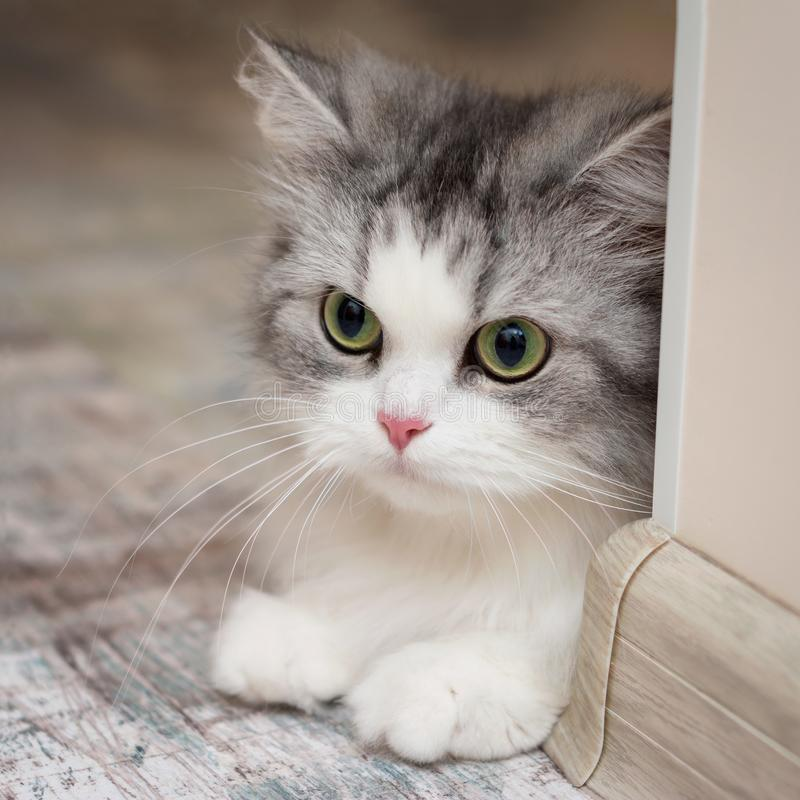
\includegraphics[width=1cm]{data/cat.png}
			};

			\matrix[every node/.style={minimum height=0.15cm, minimum width=0.15cm, draw=black, fill=green!20, inner sep=0pt}] at (1.65, 0.1) {
				\node{}; \& \node{}; \& \node{}; \& \node{}; \& \node{}; \& \node{}; \& \node{}; \& \node{};\\
				\node{}; \& \node{}; \& \node{}; \& \node{}; \& \node{}; \& \node{}; \& \node{}; \& \node{};\\
				\node{}; \& \node{}; \& \node{}; \& \node{}; \& \node{}; \& \node{}; \& \node{}; \& \node{};\\
				\node{}; \& \node{}; \& \node{}; \& \node{}; \& \node{}; \& \node{}; \& \node{}; \& \node{};\\
				\node{}; \& \node{}; \& \node{}; \& \node{}; \& \node{}; \& \node{}; \& \node{}; \& \node{};\\
				\node{}; \& \node{}; \& \node{}; \& \node{}; \& \node{}; \& \node{}; \& \node{}; \& \node{};\\
				\node{}; \& \node{}; \& \node{}; \& \node{}; \& \node{}; \& \node{}; \& \node{}; \& \node{};\\
				\node{}; \& \node{}; \& \node{}; \& \node{}; \& \node{}; \& \node{}; \& \node{}; \& \node{};\\
			};

			\matrix[every node/.style={minimum height=0.15cm, minimum width=0.15cm, draw=black, fill=green!20, inner sep=0pt, outer sep=0pt}] (l1) at (1.75, 0) {
				\node{}; \& \node{}; \& \node{}; \& \node{}; \& \node{}; \& \node{}; \& \node{}; \& \node{};\\
				\node{}; \& \node{}; \& \node{}; \& \node{}; \& \node{}; \& \node{}; \& \node{}; \& \node{};\\
				\node{}; \& \node{}; \& \node{}; \& \node{}; \& \node{}; \& \node{}; \& \node{}; \& \node{};\\
				\node{}; \& \node{}; \& \node{}; \& \node{}; \& \node{}; \& \node{}; \& \node{}; \& \node{};\\
				\node{}; \& \node{}; \& \node{}; \& \node{}; \& \node{}; \& \node{}; \& \node{}; \& \node{};\\
				\node{}; \& \node{}; \& \node{}; \& \node{}; \& \node{}; \& \node{}; \& \node{}; \& \node{};\\
				\node{}; \& \node{}; \& \node{}; \& \node{}; \& \node{}; \& \node{}; \& \node{}; \& \node{};\\
				\node{}; \& \node{}; \& \node{}; \& \node{}; \& \node{}; \& \node{}; \& \node{}; \& \node{};\\
			};
			\draw[->] (l0) -- (l1);
			\node[text depth=0] at ($(l0)!0.5!(l1) + (0, -1) $) {\tiny{Convolution}};

			\matrix[every node/.style={minimum height=0.15cm, minimum width=0.15cm, draw=black, fill=green!20, inner sep=0pt}] at (1.85, -0.1) {
				\node{}; \& \node{}; \& \node{}; \& \node{}; \& \node{}; \& \node{}; \& \node{}; \& \node{};\\
				\node{}; \& \node{}; \& \node{}; \& \node{}; \& \node{}; \& \node{}; \& \node{}; \& \node{};\\
				\node{}; \& \node{}; \& \node{}; \& \node{}; \& \node{}; \& \node{}; \& \node{}; \& \node{};\\
				\node{}; \& \node{}; \& \node{}; \& \node{}; \& \node{}; \& \node{}; \& \node{}; \& \node{};\\
				\node{}; \& \node{}; \& \node{}; \& \node{}; \& \node{}; \& \node{}; \& \node{}; \& \node{};\\
				\node{}; \& \node{}; \& \node{}; \& \node{}; \& \node{}; \& \node{}; \& \node{}; \& \node{};\\
				\node{}; \& \node{}; \& \node{}; \& \node{}; \& \node{}; \& \node{}; \& \node{}; \& \node{};\\
				\node{}; \& \node{}; \& \node{}; \& \node{}; \& \node{}; \& \node{}; \& \node{}; \& \node{};\\
			};

			\matrix[every node/.style={minimum height=0.15cm, minimum width=0.15cm, draw=black, fill=green!20, inner sep=0pt}] at (3.4, 0.1) {
				\node{}; \& \node{}; \& \node{}; \& \node{}; \& \node{}; \& \node{};\\
				\node{}; \& \node{}; \& \node{}; \& \node{}; \& \node{}; \& \node{};\\
				\node{}; \& \node{}; \& \node{}; \& \node{}; \& \node{}; \& \node{};\\
				\node{}; \& \node{}; \& \node{}; \& \node{}; \& \node{}; \& \node{};\\
				\node{}; \& \node{}; \& \node{}; \& \node{}; \& \node{}; \& \node{};\\
				\node{}; \& \node{}; \& \node{}; \& \node{}; \& \node{}; \& \node{};\\
			};

			\matrix[every node/.style={minimum height=0.15cm, minimum width=0.15cm, draw=black, fill=green!20, inner sep=0pt}] (l2)at (3.5, 0) {
				\node{}; \& \node{}; \& \node{}; \& \node{}; \& \node{}; \& \node{};\\
				\node{}; \& \node{}; \& \node{}; \& \node{}; \& \node{}; \& \node{};\\
				\node{}; \& \node{}; \& \node{}; \& \node{}; \& \node{}; \& \node{};\\
				\node{}; \& \node{}; \& \node{}; \& \node{}; \& \node{}; \& \node{};\\
				\node{}; \& \node{}; \& \node{}; \& \node{}; \& \node{}; \& \node{};\\
				\node{}; \& \node{}; \& \node{}; \& \node{}; \& \node{}; \& \node{};\\
			};
			\draw[->] (l1) -- (l2);
			\node[text depth=0] at ($(l1)!0.5!(l2) + (0, -1) $) {\tiny{Pooling}};

			\matrix[every node/.style={minimum height=0.15cm, minimum width=0.15cm, draw=black, fill=green!20, inner sep=0pt}] at (3.6, -0.1) {
				\node{}; \& \node{}; \& \node{}; \& \node{}; \& \node{}; \& \node{};\\
				\node{}; \& \node{}; \& \node{}; \& \node{}; \& \node{}; \& \node{};\\
				\node{}; \& \node{}; \& \node{}; \& \node{}; \& \node{}; \& \node{};\\
				\node{}; \& \node{}; \& \node{}; \& \node{}; \& \node{}; \& \node{};\\
				\node{}; \& \node{}; \& \node{}; \& \node{}; \& \node{}; \& \node{};\\
				\node{}; \& \node{}; \& \node{}; \& \node{}; \& \node{}; \& \node{};\\
			};

			\matrix[every node/.style={minimum height=0.15cm, minimum width=0.15cm, draw=black, fill=green!20, inner sep=0pt}] at (5.05, 0.2) {
				\node{}; \& \node{}; \& \node{}; \& \node{}; \& \node{}; \& \node{};\\
				\node{}; \& \node{}; \& \node{}; \& \node{}; \& \node{}; \& \node{};\\
				\node{}; \& \node{}; \& \node{}; \& \node{}; \& \node{}; \& \node{};\\
				\node{}; \& \node{}; \& \node{}; \& \node{}; \& \node{}; \& \node{};\\
				\node{}; \& \node{}; \& \node{}; \& \node{}; \& \node{}; \& \node{};\\
				\node{}; \& \node{}; \& \node{}; \& \node{}; \& \node{}; \& \node{};\\
			};

			\matrix[every node/.style={minimum height=0.15cm, minimum width=0.15cm, draw=black, fill=green!20, inner sep=0pt}] at (5.15, 0.1) {
				\node{}; \& \node{}; \& \node{}; \& \node{}; \& \node{}; \& \node{};\\
				\node{}; \& \node{}; \& \node{}; \& \node{}; \& \node{}; \& \node{};\\
				\node{}; \& \node{}; \& \node{}; \& \node{}; \& \node{}; \& \node{};\\
				\node{}; \& \node{}; \& \node{}; \& \node{}; \& \node{}; \& \node{};\\
				\node{}; \& \node{}; \& \node{}; \& \node{}; \& \node{}; \& \node{};\\
				\node{}; \& \node{}; \& \node{}; \& \node{}; \& \node{}; \& \node{};\\
			};

			\matrix[every node/.style={minimum height=0.15cm, minimum width=0.15cm, draw=black, fill=green!20, inner sep=0pt}] (l3) at (5.25, 0) {
				\node{}; \& \node{}; \& \node{}; \& \node{}; \& \node{}; \& \node{};\\
				\node{}; \& \node{}; \& \node{}; \& \node{}; \& \node{}; \& \node{};\\
				\node{}; \& \node{}; \& \node{}; \& \node{}; \& \node{}; \& \node{};\\
				\node{}; \& \node{}; \& \node{}; \& \node{}; \& \node{}; \& \node{};\\
				\node{}; \& \node{}; \& \node{}; \& \node{}; \& \node{}; \& \node{};\\
				\node{}; \& \node{}; \& \node{}; \& \node{}; \& \node{}; \& \node{};\\
			};
			\draw[->] (l2) -- ($ (l3.west) - (0.1, 0) $);
			\node[text depth=0] at ($(l2)!0.5!(l3) + (0, -1) $) {\tiny{Convolution}};

			\matrix[every node/.style={minimum height=0.15cm, minimum width=0.15cm, draw=black, fill=green!20, inner sep=0pt}] at (5.35, -0.1) {
				\node{}; \& \node{}; \& \node{}; \& \node{}; \& \node{}; \& \node{};\\
				\node{}; \& \node{}; \& \node{}; \& \node{}; \& \node{}; \& \node{};\\
				\node{}; \& \node{}; \& \node{}; \& \node{}; \& \node{}; \& \node{};\\
				\node{}; \& \node{}; \& \node{}; \& \node{}; \& \node{}; \& \node{};\\
				\node{}; \& \node{}; \& \node{}; \& \node{}; \& \node{}; \& \node{};\\
				\node{}; \& \node{}; \& \node{}; \& \node{}; \& \node{}; \& \node{};\\
			};

			\matrix[every node/.style={minimum height=0.15cm, minimum width=0.15cm, draw=black, fill=green!20, inner sep=0pt}] at (5.45, -0.2) {
				\node{}; \& \node{}; \& \node{}; \& \node{}; \& \node{}; \& \node{};\\
				\node{}; \& \node{}; \& \node{}; \& \node{}; \& \node{}; \& \node{};\\
				\node{}; \& \node{}; \& \node{}; \& \node{}; \& \node{}; \& \node{};\\
				\node{}; \& \node{}; \& \node{}; \& \node{}; \& \node{}; \& \node{};\\
				\node{}; \& \node{}; \& \node{}; \& \node{}; \& \node{}; \& \node{};\\
				\node{}; \& \node{}; \& \node{}; \& \node{}; \& \node{}; \& \node{};\\
			};

			\matrix[every node/.style={minimum height=0.15cm, minimum width=0.15cm, draw=black, fill=green!20, inner sep=0pt}] at (6.8, 0.2) {
				\node{}; \& \node{}; \& \node{}; \& \node{};\\
				\node{}; \& \node{}; \& \node{}; \& \node{};\\
				\node{}; \& \node{}; \& \node{}; \& \node{};\\
				\node{}; \& \node{}; \& \node{}; \& \node{};\\
			};

			\matrix[every node/.style={minimum height=0.15cm, minimum width=0.15cm, draw=black, fill=green!20, inner sep=0pt}] at (6.9, 0.1) {
				\node{}; \& \node{}; \& \node{}; \& \node{};\\
				\node{}; \& \node{}; \& \node{}; \& \node{};\\
				\node{}; \& \node{}; \& \node{}; \& \node{};\\
				\node{}; \& \node{}; \& \node{}; \& \node{};\\
			};

			\matrix[every node/.style={minimum height=0.15cm, minimum width=0.15cm, draw=black, fill=green!20, inner sep=0pt}] (l4) at (7, 0) {
				\node{}; \& \node{}; \& \node{}; \& \node{};\\
				\node{}; \& \node{}; \& \node{}; \& \node{};\\
				\node{}; \& \node{}; \& \node{}; \& \node{};\\
				\node{}; \& \node{}; \& \node{}; \& \node{};\\
			};
			\draw[->] ($ (l3.east) + (0.1, 0) $) -- ($ (l4.west) + (-0.1, 0) $);
			\node[text depth=0] at ($(l3)!0.5!(l4) + (0, -1) $) {\tiny{Pooling}};

			\matrix[every node/.style={minimum height=0.15cm, minimum width=0.15cm, draw=black, fill=green!20, inner sep=0pt}] at (7.1, -0.1) {
				\node{}; \& \node{}; \& \node{}; \& \node{};\\
				\node{}; \& \node{}; \& \node{}; \& \node{};\\
				\node{}; \& \node{}; \& \node{}; \& \node{};\\
				\node{}; \& \node{}; \& \node{}; \& \node{};\\
			};
			\matrix[every node/.style={minimum height=0.15cm, minimum width=0.15cm, draw=black, fill=green!20, inner sep=0pt}] at (7.2, -0.2) {
				\node{}; \& \node{}; \& \node{}; \& \node{};\\
				\node{}; \& \node{}; \& \node{}; \& \node{};\\
				\node{}; \& \node{}; \& \node{}; \& \node{};\\
				\node{}; \& \node{}; \& \node{}; \& \node{};\\
			};

			\matrix[every node/.style={minimum height=0.15cm, minimum width=0.15cm, draw=black, fill=green!20, inner sep=0pt}] at (8.25, 0.3) {
				\node{}; \& \node{}; \& \node{}; \& \node{};\\
				\node{}; \& \node{}; \& \node{}; \& \node{};\\
				\node{}; \& \node{}; \& \node{}; \& \node{};\\
				\node{}; \& \node{}; \& \node{}; \& \node{};\\
			};

			\matrix[every node/.style={minimum height=0.15cm, minimum width=0.15cm, draw=black, fill=green!20, inner sep=0pt}] at (8.35, 0.2) {
				\node{}; \& \node{}; \& \node{}; \& \node{};\\
				\node{}; \& \node{}; \& \node{}; \& \node{};\\
				\node{}; \& \node{}; \& \node{}; \& \node{};\\
				\node{}; \& \node{}; \& \node{}; \& \node{};\\
			};

			\matrix[every node/.style={minimum height=0.15cm, minimum width=0.15cm, draw=black, fill=green!20, inner sep=0pt}] at (8.45, 0.1) {
				\node{}; \& \node{}; \& \node{}; \& \node{};\\
				\node{}; \& \node{}; \& \node{}; \& \node{};\\
				\node{}; \& \node{}; \& \node{}; \& \node{};\\
				\node{}; \& \node{}; \& \node{}; \& \node{};\\
			};

			\matrix[every node/.style={minimum height=0.15cm, minimum width=0.15cm, draw=black, fill=green!20, inner sep=0pt}] (l5) at (8.55, 0) {
				\node{}; \& \node{}; \& \node{}; \& \node{};\\
				\node{}; \& \node{}; \& \node{}; \& \node{};\\
				\node{}; \& \node{}; \& \node{}; \& \node{};\\
				\node{}; \& \node{}; \& \node{}; \& \node{};\\
			};
			\draw[->] ($ (l4.east) + (0.1, 0) $) -- ($ (l5.west) + (-0.2, 0) $);
			\node[text depth=0] at ($(l4)!0.5!(l5) + (0, -1) $) {\tiny{Convolution}};

			\matrix[every node/.style={minimum height=0.15cm, minimum width=0.15cm, draw=black, fill=green!20, inner sep=0pt}] at (8.65, -0.1) {
				\node{}; \& \node{}; \& \node{}; \& \node{};\\
				\node{}; \& \node{}; \& \node{}; \& \node{};\\
				\node{}; \& \node{}; \& \node{}; \& \node{};\\
				\node{}; \& \node{}; \& \node{}; \& \node{};\\
			};

			\matrix[every node/.style={minimum height=0.15cm, minimum width=0.15cm, draw=black, fill=green!20, inner sep=0pt}] at (8.75, -0.2) {
				\node{}; \& \node{}; \& \node{}; \& \node{};\\
				\node{}; \& \node{}; \& \node{}; \& \node{};\\
				\node{}; \& \node{}; \& \node{}; \& \node{};\\
				\node{}; \& \node{}; \& \node{}; \& \node{};\\
			};

			\matrix[every node/.style={minimum height=0.15cm, minimum width=0.15cm, draw=black, fill=green!20, inner sep=0pt}] at (8.85, -0.3) {
				\node{}; \& \node{}; \& \node{}; \& \node{};\\
				\node{}; \& \node{}; \& \node{}; \& \node{};\\
				\node{}; \& \node{}; \& \node{}; \& \node{};\\
				\node{}; \& \node{}; \& \node{}; \& \node{};\\
			};


			\node[circle, draw=black, fill=green!20, text depth=0, inner sep=2pt] (y1) at (10.5, 0.125) {\tiny{$y_0$}};
			\node[circle, draw=black, fill=green!20, text depth=0, inner sep=2pt] (y2) at (10.75, -0.125) {\tiny{$y_1$}};

			\node[minimum height=0.15cm, minimum width=0.15cm, draw=black, fill=green!20, inner sep=0pt] (n0) at (9.4, 0.3) {};
			\draw[->] (n0) -- (y1);
			\node[minimum height=0.15cm, minimum width=0.15cm, draw=black, fill=green!20, inner sep=0pt] (n1) at (9.5, 0.2) {};
			\draw[->] (n1) -- (y1);
			\node[minimum height=0.15cm, minimum width=0.15cm, draw=black, fill=green!20, inner sep=0pt] (n2) at (9.6, 0.1) {};
			\draw[->] (n2) -- (y1);
			\node[minimum height=0.15cm, minimum width=0.15cm, draw=black, fill=green!20, inner sep=0pt] (n3) at (9.7, 0) {};
			\draw[->] ($ (l5.east) + (0.2, 0) $) -- ($ (n3.west) + (-0.15, 0) $);
			\node[text depth=0] at ($(l5)!0.5!(n3) + (0, -1) $) {\tiny{Pooling}};
			\draw[->] (n3) -- (y1);
			\node[minimum height=0.15cm, minimum width=0.15cm, draw=black, fill=green!20, inner sep=0pt] (n4) at (9.8, -0.1) {};
			\draw[->] (n4) -- (y1);
			\node[minimum height=0.15cm, minimum width=0.15cm, draw=black, fill=green!20, inner sep=0pt] (n5) at (9.9, -0.2) {};
			\draw[->] (n5) -- (y1);
			\node[minimum height=0.15cm, minimum width=0.15cm, draw=black, fill=green!20, inner sep=0pt] (n6) at (10, -0.3) {};
			\draw[->] (n6) -- (y1);

			\node[minimum height=0.15cm, minimum width=0.15cm, draw=black, fill=green!20, inner sep=0pt] (n0) at (9.4, 0.3) {};
			\draw[->] (n0) -- (y2);
			\node[minimum height=0.15cm, minimum width=0.15cm, draw=black, fill=green!20, inner sep=0pt] (n1) at (9.5, 0.2) {};
			\draw[->] (n1) -- (y2);
			\node[minimum height=0.15cm, minimum width=0.15cm, draw=black, fill=green!20, inner sep=0pt] (n2) at (9.6, 0.1) {};
			\draw[->] (n2) -- (y2);
			\node[minimum height=0.15cm, minimum width=0.15cm, draw=black, fill=green!20, inner sep=0pt] (n3) at (9.7, 0) {};
			\draw[->] (n3) -- (y2);
			\node[minimum height=0.15cm, minimum width=0.15cm, draw=black, fill=green!20, inner sep=0pt] (n4) at (9.8, -0.1) {};
			\draw[->] (n4) -- (y2);
			\node[minimum height=0.15cm, minimum width=0.15cm, draw=black, fill=green!20, inner sep=0pt] (n5) at (9.9, -0.2) {};
			\draw[->] (n5) -- (y2);
			\node[minimum height=0.15cm, minimum width=0.15cm, draw=black, fill=green!20, inner sep=0pt] (n6) at (10, -0.3) {};
			\draw[->] (n6) -- (y2);

		\end{tikzpicture}
		}
		\vfill
	\end{frame}

	\begin{frame}{Teori: Konvolusjonelle nevrale nettverk} % Patterns
		\centering
		\vfill
		\resizebox{\textwidth}{!}{
		\begin{tikzpicture}[
			ampersand replacement=\&
		]
			\node[inner sep=0pt, draw=black] (l0) at (0, 0) {
				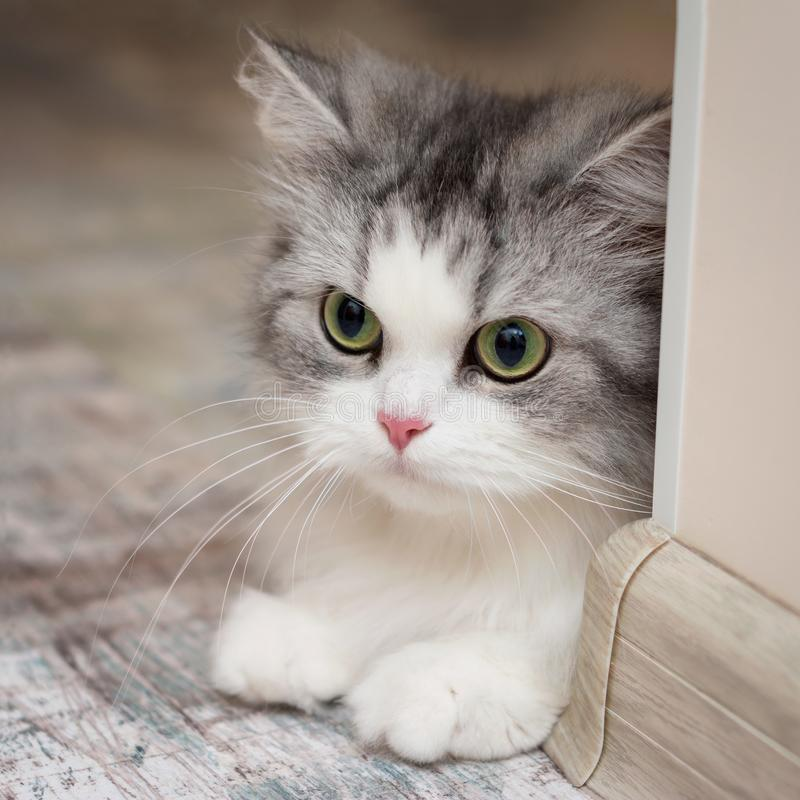
\includegraphics[width=1cm]{data/cat.png}
			};

			\matrix[every node/.style={minimum height=0.15cm, minimum width=0.15cm, draw=black, fill=green!20, inner sep=0pt}] at (1.65, 0.1) {
				\node{}; \& \node{}; \& \node{}; \& \node{}; \& \node{}; \& \node{}; \& \node{}; \& \node{};\\
				\node{}; \& \node{}; \& \node{}; \& \node{}; \& \node{}; \& \node{}; \& \node{}; \& \node{};\\
				\node{}; \& \node{}; \& \node{}; \& \node{}; \& \node{}; \& \node{}; \& \node{}; \& \node{};\\
				\node{}; \& \node{}; \& \node{}; \& \node{}; \& \node{}; \& \node{}; \& \node{}; \& \node{};\\
				\node{}; \& \node{}; \& \node{}; \& \node{}; \& \node{}; \& \node{}; \& \node{}; \& \node{};\\
				\node{}; \& \node{}; \& \node{}; \& \node{}; \& \node{}; \& \node{}; \& \node{}; \& \node{};\\
				\node{}; \& \node{}; \& \node{}; \& \node{}; \& \node{}; \& \node{}; \& \node{}; \& \node{};\\
				\node{}; \& \node{}; \& \node{}; \& \node{}; \& \node{}; \& \node{}; \& \node{}; \& \node{};\\
			};

			\matrix[every node/.style={minimum height=0.15cm, minimum width=0.15cm, draw=black, fill=green!20, inner sep=0pt, outer sep=0pt}] (l1) at (1.75, 0) {
				\node{}; \& \node{}; \& \node{}; \& \node{}; \& \node{}; \& \node{}; \& \node{}; \& \node{};\\
				\node{}; \& \node{}; \& \node{}; \& \node{}; \& \node{}; \& \node{}; \& \node{}; \& \node{};\\
				\node{}; \& \node{}; \& \node{}; \& \node{}; \& \node{}; \& \node{}; \& \node{}; \& \node{};\\
				\node{}; \& \node{}; \& \node{}; \& \node{}; \& \node{}; \& \node{}; \& \node{}; \& \node{};\\
				\node{}; \& \node{}; \& \node{}; \& \node{}; \& \node{}; \& \node{}; \& \node{}; \& \node{};\\
				\node{}; \& \node{}; \& \node{}; \& \node{}; \& \node{}; \& \node{}; \& \node{}; \& \node{};\\
				\node{}; \& \node{}; \& \node{}; \& \node{}; \& \node{}; \& \node{}; \& \node{}; \& \node{};\\
				\node{}; \& \node{}; \& \node{}; \& \node{}; \& \node{}; \& \node{}; \& \node{}; \& \node{};\\
			};
			\draw[->] (l0) -- (l1);
			\node[text depth=0] at ($(l0)!0.5!(l1) + (0, -1) $) {\tiny{Convolution}};

			\matrix[every node/.style={minimum height=0.15cm, minimum width=0.15cm, draw=black, fill=green!20, inner sep=0pt}] at (1.85, -0.1) {
				\node{}; \& \node{}; \& \node{}; \& \node{}; \& \node{}; \& \node{}; \& \node{}; \& \node{};\\
				\node{}; \& \node{}; \& \node{}; \& \node{}; \& \node{}; \& \node{}; \& \node{}; \& \node{};\\
				\node{}; \& \node{}; \& \node{}; \& \node{}; \& \node{}; \& \node{}; \& \node{}; \& \node{};\\
				\node{}; \& \node{}; \& \node{}; \& \node{}; \& \node{}; \& \node{}; \& \node{}; \& \node{};\\
				\node{}; \& \node{}; \& \node{}; \& \node{}; \& \node{}; \& \node{}; \& \node{}; \& \node{};\\
				\node{}; \& \node{}; \& \node{}; \& \node{}; \& \node{}; \& \node{}; \& \node{}; \& \node{};\\
				\node{}; \& \node{}; \& \node{}; \& \node{}; \& \node{}; \& \node{}; \& \node{}; \& \node{};\\
				\node{}; \& \node{}; \& \node{}; \& \node{}; \& \node{}; \& \node{}; \& \node{}; \& \node{};\\
			};

			\matrix[every node/.style={minimum height=0.15cm, minimum width=0.15cm, draw=black, fill=green!20, inner sep=0pt}] at (3.4, 0.1) {
				\node{}; \& \node{}; \& \node{}; \& \node{}; \& \node{}; \& \node{};\\
				\node{}; \& \node{}; \& \node{}; \& \node{}; \& \node{}; \& \node{};\\
				\node{}; \& \node{}; \& \node{}; \& \node{}; \& \node{}; \& \node{};\\
				\node{}; \& \node{}; \& \node{}; \& \node{}; \& \node{}; \& \node{};\\
				\node{}; \& \node{}; \& \node{}; \& \node{}; \& \node{}; \& \node{};\\
				\node{}; \& \node{}; \& \node{}; \& \node{}; \& \node{}; \& \node{};\\
			};

			\matrix[every node/.style={minimum height=0.15cm, minimum width=0.15cm, draw=black, fill=green!20, inner sep=0pt}] (l2)at (3.5, 0) {
				\node{}; \& \node{}; \& \node{}; \& \node{}; \& \node{}; \& \node{};\\
				\node{}; \& \node{}; \& \node{}; \& \node{}; \& \node{}; \& \node{};\\
				\node{}; \& \node{}; \& \node{}; \& \node{}; \& \node{}; \& \node{};\\
				\node{}; \& \node{}; \& \node{}; \& \node{}; \& \node{}; \& \node{};\\
				\node{}; \& \node{}; \& \node{}; \& \node{}; \& \node{}; \& \node{};\\
				\node{}; \& \node{}; \& \node{}; \& \node{}; \& \node{}; \& \node{};\\
			};
			\draw[->] (l1) -- (l2);
			\node[text depth=0] at ($(l1)!0.5!(l2) + (0, -1) $) {\tiny{Pooling}};

			\matrix[every node/.style={minimum height=0.15cm, minimum width=0.15cm, draw=black, fill=green!20, inner sep=0pt}] at (3.6, -0.1) {
				\node{}; \& \node{}; \& \node{}; \& \node{}; \& \node{}; \& \node{};\\
				\node{}; \& \node{}; \& \node{}; \& \node{}; \& \node{}; \& \node{};\\
				\node{}; \& \node{}; \& \node{}; \& \node{}; \& \node{}; \& \node{};\\
				\node{}; \& \node{}; \& \node{}; \& \node{}; \& \node{}; \& \node{};\\
				\node{}; \& \node{}; \& \node{}; \& \node{}; \& \node{}; \& \node{};\\
				\node{}; \& \node{}; \& \node{}; \& \node{}; \& \node{}; \& \node{};\\
			};

			\matrix[every node/.style={minimum height=0.15cm, minimum width=0.15cm, draw=black, fill=green!20, inner sep=0pt}] at (5.05, 0.2) {
				\node{}; \& \node{}; \& \node{}; \& \node{}; \& \node{}; \& \node{};\\
				\node{}; \& \node{}; \& \node{}; \& \node{}; \& \node{}; \& \node{};\\
				\node{}; \& \node{}; \& \node{}; \& \node{}; \& \node{}; \& \node{};\\
				\node{}; \& \node{}; \& \node{}; \& \node{}; \& \node{}; \& \node{};\\
				\node{}; \& \node{}; \& \node{}; \& \node{}; \& \node{}; \& \node{};\\
				\node{}; \& \node{}; \& \node{}; \& \node{}; \& \node{}; \& \node{};\\
			};

			\matrix[every node/.style={minimum height=0.15cm, minimum width=0.15cm, draw=black, fill=green!20, inner sep=0pt}] at (5.15, 0.1) {
				\node{}; \& \node{}; \& \node{}; \& \node{}; \& \node{}; \& \node{};\\
				\node{}; \& \node{}; \& \node{}; \& \node{}; \& \node{}; \& \node{};\\
				\node{}; \& \node{}; \& \node{}; \& \node{}; \& \node{}; \& \node{};\\
				\node{}; \& \node{}; \& \node{}; \& \node{}; \& \node{}; \& \node{};\\
				\node{}; \& \node{}; \& \node{}; \& \node{}; \& \node{}; \& \node{};\\
				\node{}; \& \node{}; \& \node{}; \& \node{}; \& \node{}; \& \node{};\\
			};

			\matrix[every node/.style={minimum height=0.15cm, minimum width=0.15cm, draw=black, fill=green!20, inner sep=0pt}] (l3) at (5.25, 0) {
				\node{}; \& \node{}; \& \node{}; \& \node{}; \& \node{}; \& \node{};\\
				\node{}; \& \node{}; \& \node{}; \& \node{}; \& \node{}; \& \node{};\\
				\node{}; \& \node{}; \& \node{}; \& \node{}; \& \node{}; \& \node{};\\
				\node{}; \& \node{}; \& \node{}; \& \node{}; \& \node{}; \& \node{};\\
				\node{}; \& \node{}; \& \node{}; \& \node{}; \& \node{}; \& \node{};\\
				\node{}; \& \node{}; \& \node{}; \& \node{}; \& \node{}; \& \node{};\\
			};
			\draw[->] (l2) -- ($ (l3.west) - (0.1, 0) $);
			\node[text depth=0] at ($(l2)!0.5!(l3) + (0, -1) $) {\tiny{Convolution}};

			\matrix[every node/.style={minimum height=0.15cm, minimum width=0.15cm, draw=black, fill=green!20, inner sep=0pt}] at (5.35, -0.1) {
				\node{}; \& \node{}; \& \node{}; \& \node{}; \& \node{}; \& \node{};\\
				\node{}; \& \node{}; \& \node{}; \& \node{}; \& \node{}; \& \node{};\\
				\node{}; \& \node{}; \& \node{}; \& \node{}; \& \node{}; \& \node{};\\
				\node{}; \& \node{}; \& \node{}; \& \node{}; \& \node{}; \& \node{};\\
				\node{}; \& \node{}; \& \node{}; \& \node{}; \& \node{}; \& \node{};\\
				\node{}; \& \node{}; \& \node{}; \& \node{}; \& \node{}; \& \node{};\\
			};

			\matrix[every node/.style={minimum height=0.15cm, minimum width=0.15cm, draw=black, fill=green!20, inner sep=0pt}] at (5.45, -0.2) {
				\node{}; \& \node{}; \& \node{}; \& \node{}; \& \node{}; \& \node{};\\
				\node{}; \& \node{}; \& \node{}; \& \node{}; \& \node{}; \& \node{};\\
				\node{}; \& \node{}; \& \node{}; \& \node{}; \& \node{}; \& \node{};\\
				\node{}; \& \node{}; \& \node{}; \& \node{}; \& \node{}; \& \node{};\\
				\node{}; \& \node{}; \& \node{}; \& \node{}; \& \node{}; \& \node{};\\
				\node{}; \& \node{}; \& \node{}; \& \node{}; \& \node{}; \& \node{};\\
			};

			\matrix[every node/.style={minimum height=0.15cm, minimum width=0.15cm, draw=black, fill=green!20, inner sep=0pt}] at (6.8, 0.2) {
				\node{}; \& \node{}; \& \node{}; \& \node{};\\
				\node{}; \& \node{}; \& \node{}; \& \node{};\\
				\node{}; \& \node{}; \& \node{}; \& \node{};\\
				\node{}; \& \node{}; \& \node{}; \& \node{};\\
			};

			\matrix[every node/.style={minimum height=0.15cm, minimum width=0.15cm, draw=black, fill=green!20, inner sep=0pt}] at (6.9, 0.1) {
				\node{}; \& \node{}; \& \node{}; \& \node{};\\
				\node{}; \& \node{}; \& \node{}; \& \node{};\\
				\node{}; \& \node{}; \& \node{}; \& \node{};\\
				\node{}; \& \node{}; \& \node{}; \& \node{};\\
			};

			\matrix[every node/.style={minimum height=0.15cm, minimum width=0.15cm, draw=black, fill=green!20, inner sep=0pt}] (l4) at (7, 0) {
				\node{}; \& \node{}; \& \node{}; \& \node{};\\
				\node{}; \& \node{}; \& \node{}; \& \node{};\\
				\node{}; \& \node{}; \& \node{}; \& \node{};\\
				\node{}; \& \node{}; \& \node{}; \& \node{};\\
			};
			\draw[->] ($ (l3.east) + (0.1, 0) $) -- ($ (l4.west) + (-0.1, 0) $);
			\node[text depth=0] at ($(l3)!0.5!(l4) + (0, -1) $) {\tiny{Pooling}};

			\matrix[every node/.style={minimum height=0.15cm, minimum width=0.15cm, draw=black, fill=green!20, inner sep=0pt}] at (7.1, -0.1) {
				\node{}; \& \node{}; \& \node{}; \& \node{};\\
				\node{}; \& \node{}; \& \node{}; \& \node{};\\
				\node{}; \& \node{}; \& \node{}; \& \node{};\\
				\node{}; \& \node{}; \& \node{}; \& \node{};\\
			};
			\matrix[every node/.style={minimum height=0.15cm, minimum width=0.15cm, draw=black, fill=green!20, inner sep=0pt}] at (7.2, -0.2) {
				\node{}; \& \node{}; \& \node{}; \& \node{};\\
				\node{}; \& \node{}; \& \node{}; \& \node{};\\
				\node{}; \& \node{}; \& \node{}; \& \node{};\\
				\node{}; \& \node{}; \& \node{}; \& \node{};\\
			};

			\matrix[every node/.style={minimum height=0.15cm, minimum width=0.15cm, draw=black, fill=green!20, inner sep=0pt}] at (8.25, 0.3) {
				\node{}; \& \node{}; \& \node{}; \& \node{};\\
				\node{}; \& \node{}; \& \node{}; \& \node{};\\
				\node{}; \& \node{}; \& \node{}; \& \node{};\\
				\node{}; \& \node{}; \& \node{}; \& \node{};\\
			};

			\matrix[every node/.style={minimum height=0.15cm, minimum width=0.15cm, draw=black, fill=green!20, inner sep=0pt}] at (8.35, 0.2) {
				\node{}; \& \node{}; \& \node{}; \& \node{};\\
				\node{}; \& \node{}; \& \node{}; \& \node{};\\
				\node{}; \& \node{}; \& \node{}; \& \node{};\\
				\node{}; \& \node{}; \& \node{}; \& \node{};\\
			};

			\matrix[every node/.style={minimum height=0.15cm, minimum width=0.15cm, draw=black, fill=green!20, inner sep=0pt}] at (8.45, 0.1) {
				\node{}; \& \node{}; \& \node{}; \& \node{};\\
				\node{}; \& \node{}; \& \node{}; \& \node{};\\
				\node{}; \& \node{}; \& \node{}; \& \node{};\\
				\node{}; \& \node{}; \& \node{}; \& \node{};\\
			};

			\matrix[every node/.style={minimum height=0.15cm, minimum width=0.15cm, draw=black, fill=green!20, inner sep=0pt}] (l5) at (8.55, 0) {
				\node{}; \& \node{}; \& \node{}; \& \node{};\\
				\node{}; \& \node{}; \& \node{}; \& \node{};\\
				\node{}; \& \node{}; \& \node{}; \& \node{};\\
				\node{}; \& \node{}; \& \node{}; \& \node{};\\
			};
			\draw[->] ($ (l4.east) + (0.1, 0) $) -- ($ (l5.west) + (-0.2, 0) $);
			\node[text depth=0] at ($(l4)!0.5!(l5) + (0, -1) $) {\tiny{Convolution}};

			\matrix[every node/.style={minimum height=0.15cm, minimum width=0.15cm, draw=black, fill=green!20, inner sep=0pt}] at (8.65, -0.1) {
				\node{}; \& \node{}; \& \node{}; \& \node{};\\
				\node{}; \& \node{}; \& \node{}; \& \node{};\\
				\node{}; \& \node{}; \& \node{}; \& \node{};\\
				\node{}; \& \node{}; \& \node{}; \& \node{};\\
			};

			\matrix[every node/.style={minimum height=0.15cm, minimum width=0.15cm, draw=black, fill=green!20, inner sep=0pt}] at (8.75, -0.2) {
				\node{}; \& \node{}; \& \node{}; \& \node{};\\
				\node{}; \& \node{}; \& \node{}; \& \node{};\\
				\node{}; \& \node{}; \& \node{}; \& \node{};\\
				\node{}; \& \node{}; \& \node{}; \& \node{};\\
			};

			\matrix[every node/.style={minimum height=0.15cm, minimum width=0.15cm, draw=black, fill=green!20, inner sep=0pt}] at (8.85, -0.3) {
				\node{}; \& \node{}; \& \node{}; \& \node{};\\
				\node{}; \& \node{}; \& \node{}; \& \node{};\\
				\node{}; \& \node{}; \& \node{}; \& \node{};\\
				\node{}; \& \node{}; \& \node{}; \& \node{};\\
			};


			\node[circle, draw=black, fill=green!20, text depth=0, inner sep=2pt] (y1) at (10.5, 0.125) {\tiny{$y_0$}};
			\node[circle, draw=black, fill=green!20, text depth=0, inner sep=2pt] (y2) at (10.75, -0.125) {\tiny{$y_1$}};

			\node[minimum height=0.15cm, minimum width=0.15cm, draw=black, fill=green!20, inner sep=0pt] (n0) at (9.4, 0.3) {};
			\draw[->] (n0) -- (y1);
			\node[minimum height=0.15cm, minimum width=0.15cm, draw=black, fill=green!20, inner sep=0pt] (n1) at (9.5, 0.2) {};
			\draw[->] (n1) -- (y1);
			\node[minimum height=0.15cm, minimum width=0.15cm, draw=black, fill=green!20, inner sep=0pt] (n2) at (9.6, 0.1) {};
			\draw[->] (n2) -- (y1);
			\node[minimum height=0.15cm, minimum width=0.15cm, draw=black, fill=green!20, inner sep=0pt] (n3) at (9.7, 0) {};
			\draw[->] ($ (l5.east) + (0.2, 0) $) -- ($ (n3.west) + (-0.15, 0) $);
			\node[text depth=0] at ($(l5)!0.5!(n3) + (0, -1) $) {\tiny{Pooling}};
			\draw[->] (n3) -- (y1);
			\node[minimum height=0.15cm, minimum width=0.15cm, draw=black, fill=green!20, inner sep=0pt] (n4) at (9.8, -0.1) {};
			\draw[->] (n4) -- (y1);
			\node[minimum height=0.15cm, minimum width=0.15cm, draw=black, fill=green!20, inner sep=0pt] (n5) at (9.9, -0.2) {};
			\draw[->] (n5) -- (y1);
			\node[minimum height=0.15cm, minimum width=0.15cm, draw=black, fill=green!20, inner sep=0pt] (n6) at (10, -0.3) {};
			\draw[->] (n6) -- (y1);

			\node[minimum height=0.15cm, minimum width=0.15cm, draw=black, fill=green!20, inner sep=0pt] (n0) at (9.4, 0.3) {};
			\draw[->] (n0) -- (y2);
			\node[minimum height=0.15cm, minimum width=0.15cm, draw=black, fill=green!20, inner sep=0pt] (n1) at (9.5, 0.2) {};
			\draw[->] (n1) -- (y2);
			\node[minimum height=0.15cm, minimum width=0.15cm, draw=black, fill=green!20, inner sep=0pt] (n2) at (9.6, 0.1) {};
			\draw[->] (n2) -- (y2);
			\node[minimum height=0.15cm, minimum width=0.15cm, draw=black, fill=green!20, inner sep=0pt] (n3) at (9.7, 0) {};
			\draw[->] (n3) -- (y2);
			\node[minimum height=0.15cm, minimum width=0.15cm, draw=black, fill=green!20, inner sep=0pt] (n4) at (9.8, -0.1) {};
			\draw[->] (n4) -- (y2);
			\node[minimum height=0.15cm, minimum width=0.15cm, draw=black, fill=green!20, inner sep=0pt] (n5) at (9.9, -0.2) {};
			\draw[->] (n5) -- (y2);
			\node[minimum height=0.15cm, minimum width=0.15cm, draw=black, fill=green!20, inner sep=0pt] (n6) at (10, -0.3) {};
			\draw[->] (n6) -- (y2);

			\node[text depth=0] at ($(l0)!0.5!(l1) + (0, -3) $) {
				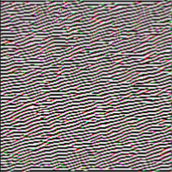
\includegraphics[height=2cm, width=2cm]{data/first.png}
			};

			\node[text depth=0] at ($(l2)!0.5!(l3) + (0, -3) $) {
				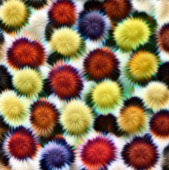
\includegraphics[height=2cm, width=2cm]{data/third.png}
			};

			\node[text depth=0] at ($(l4)!0.5!(l5) + (0, -3) $) {
				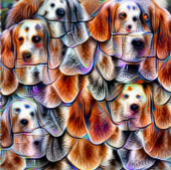
\includegraphics[height=2cm, width=2cm]{data/fifth.png}
			};

			\end{tikzpicture}
		}
		\vfill
	\end{frame}

	\section{AI i hjerneforskning}

	\begin{frame}{AI i hjerneforskning: Oversikt}
		\centering
		\begin{tikzpicture}
			\node[inner sep=0pt, label=below:{Artikler om dyplæring i medisin per år}, draw=black] {
				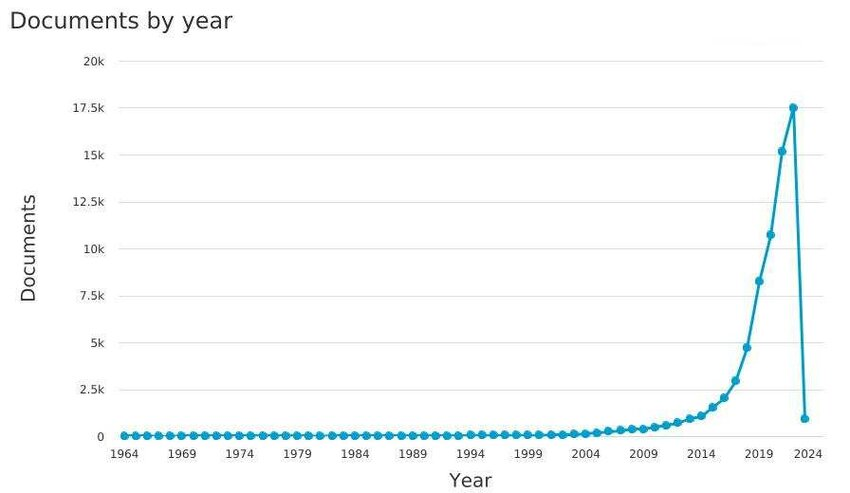
\includegraphics[width=8cm]{data/scopus.png}
			};
		\end{tikzpicture}
	\end{frame}

	\begin{frame}[b]{AI i hjerneforskning: Segmentering}
		\centering
		\begin{tikzpicture}
			\node[draw=black] {
				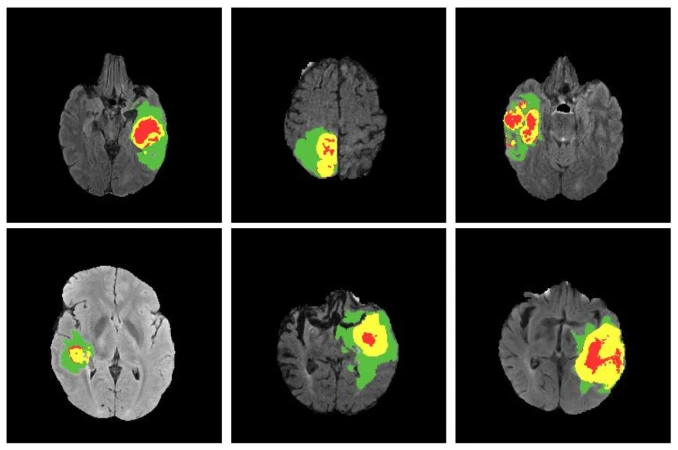
\includegraphics[width=8cm]{data/glioblastoma.png}
			};
		\end{tikzpicture}\\
		\vspace{1cm}
		Segmentering av hjernesvulster (glioblastoma) basert på MR-bilder
	\end{frame}

	\begin{frame}{AI i hjerneforskning: Diagnostisk klassifisering} % Prediction
		\centering
		\begin{tikzpicture}
          \newcommand{\mrivsep}{0.52}
			\newcommand{\mrihsep}{0.44}
			\def\plotwidth{11.68}

			\newcommand{\nodesize}{11pt}
			\newcommand{\hsep}{28pt}
			\newcommand{\vsep}{14pt}

			\newcommand{\arrowwidth}{0.05cm}
			\newcommand{\innerarrow}{{Latex[length=0.1cm, width=0.15cm]}}
			\newcommand{\outerarrow}{{Latex[length=0.2cm, width=0.3cm]}}

			\definecolor{cb-green}{HTML}{4dac93}
			\definecolor{cb-blue}{HTML}{3594d6}
			\definecolor{outercolor}{RGB}{128, 128, 128}
			\colorlet{train-fill}{cb-blue}

			\newcommand{\patientlocation}[1]{($ (1, -1.6) + ####1 $)}
			\newcommand{\controllocation}[1]{($ (1, -2.8) + ####1 $)}
			\newcommand{\modellocation}[1]{($ (0.5 * \plotwidth, -2.2) + ####1 $)}

			\node[draw=none, outer sep=0pt, inner sep=0pt] (input) at \modellocation{(-4.5 * \hsep, 0)} {
				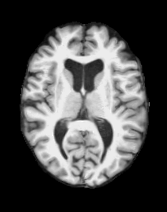
\includegraphics[width=1.5cm] {
					data/mris/control_0.png
				}
			};

			\node[circle, inner sep=0pt, fill=none, outer sep=0pt, line width=0pt, draw=none] (n00) at \modellocation{(-3 * \hsep, 0)} {};

			\node[circle, minimum size=\nodesize, inner sep=0pt, fill=train-fill!35, outer sep=0pt, line width=0pt, draw=train-fill!35] (n10) at \modellocation{(-2 * \hsep, 2 * \vsep)} {};
			\node[circle, minimum size=\nodesize, inner sep=0pt, fill=train-fill, outer sep=0pt, line width=0pt, draw=train-fill] (n11) at \modellocation{(-2 * \hsep, 1 * \vsep)} {};
			\node[circle, minimum size=\nodesize, inner sep=0pt, fill=train-fill!15, outer sep=0pt, line width=0pt, draw=train-fill!15] (n12) at \modellocation{(-2 * \hsep, 0)} {};
			\node[circle, minimum size=\nodesize, inner sep=0pt, fill=train-fill!85, outer sep=0pt, line width=0pt, draw=train-fill!85] (n13) at \modellocation{(-2 * \hsep, -1 * \vsep)} {};
			\node[circle, minimum size=\nodesize, inner sep=0pt, fill=train-fill!90, outer sep=0pt, line width=0pt, draw=train-fill!90] (n14) at \modellocation{(-2 * \hsep, -2 * \vsep)} {};

			\node[circle, minimum size=\nodesize, inner sep=0pt, fill=train-fill!55, outer sep=0pt, line width=0pt, draw=train-fill!55] (n20) at \modellocation{(-1 * \hsep, 1.5 * \vsep)} {};
			\node[circle, minimum size=\nodesize, inner sep=0pt, fill=train-fill!20, outer sep=0pt, line width=0pt, draw=train-fill!20] (n21) at \modellocation{(-1 * \hsep, 0.5 * \vsep)} {};
			\node[circle, minimum size=\nodesize, inner sep=0pt, fill=train-fill!90, outer sep=0pt, line width=0pt, draw=train-fill!50] (n22) at \modellocation{(-1 * \hsep, -0.5 * \vsep)} {};
			\node[circle, minimum size=\nodesize, inner sep=0pt, fill=train-fill!35, outer sep=0pt, line width=0pt, draw=train-fill!35] (n23) at \modellocation{(-1 * \hsep, -1.5 * \vsep)} {};

			\node[circle, minimum size=\nodesize, inner sep=0pt, fill=train-fill!95, outer sep=0pt, line width=0pt, draw=train-fill!65] (n30) at \modellocation{(0 * \hsep, 1.5 * \vsep)} {};
			\node[circle, minimum size=\nodesize, inner sep=0pt, fill=train-fill!20, outer sep=0pt, line width=0pt, draw=train-fill!20] (n31) at \modellocation{(0 * \hsep, 0.5 * \vsep)} {};
			\node[circle, minimum size=\nodesize, inner sep=0pt, fill=train-fill!90, outer sep=0pt, line width=0pt, draw=train-fill!90] (n32) at \modellocation{(0 * \hsep, -0.5 * \vsep)} {};
			\node[circle, minimum size=\nodesize, inner sep=0pt, fill=train-fill!80, outer sep=0pt, line width=0pt, draw=train-fill!80] (n33) at \modellocation{(0 * \hsep, -1.5 * \vsep)} {};

			\node[circle, minimum size=\nodesize, inner sep=0pt, fill=train-fill!50, outer sep=0pt, line width=0pt, draw=train-fill!50] (n40) at \modellocation{(1 * \hsep, 1*\vsep)} {};
			\node[circle, minimum size=\nodesize, inner sep=0pt, fill=train-fill!90, outer sep=0pt, line width=0pt, draw=train-fill!70] (n41) at \modellocation{(1 * \hsep, 0*\vsep)} {};
			\node[circle, minimum size=\nodesize, inner sep=0pt, fill=train-fill!70, outer sep=0pt, line width=0pt, draw=train-fill!30] (n42) at \modellocation{(1 * \hsep, -1*\vsep)} {};

			\node[circle, minimum size=\nodesize, inner sep=0pt, fill=train-fill, outer sep=0pt, line width=0pt, draw=train-fill] (n50) at \modellocation{(2 * \hsep, 1*\vsep)} {};
			\node[circle, minimum size=\nodesize, inner sep=0pt, fill=train-fill!70, outer sep=0pt, line width=0pt, draw=train-fill!70] (n51) at \modellocation{(2 * \hsep, 0*\vsep)} {};
			\node[circle, minimum size=\nodesize, inner sep=0pt, fill=train-fill!30, outer sep=0pt, line width=0pt, draw=train-fill!30] (n52) at \modellocation{(2 * \hsep, -1*\vsep)} {};

			\node[circle, minimum size=\nodesize, inner sep=0pt, fill=train-fill!80, outer sep=0pt, line width=0pt, draw=train-fill!65] (n60) at \modellocation{(3 * \hsep, 0)} {};

			\node[align=left, font=\linespread{0.8}\selectfont] (loss) at (0.2+2.1*4.85, -2.2) {Diagnose};

			\draw[
				color=train-fill!35,
				-\innerarrow,
				line width=\arrowwidth
			] (n00) to [out=20,in=200] (n10) {};
			\draw[
				color=train-fill,
				-\innerarrow,
				line width=\arrowwidth
			] (n00) to [out=10,in=190] (n11) {};
			\draw[
				color=train-fill!15,
				-\innerarrow,
				line width=\arrowwidth
			] (n00) to [out=0,in=180] (n12) {};
			\draw[
				color=train-fill!85,
				-\innerarrow,
				line width=\arrowwidth
			] (n00) to [out=-10,in=170] (n13) {};
			\draw[
				color=train-fill!90,
				-\innerarrow,
				line width=\arrowwidth
			] (n00) to [out=-20,in=160] (n14) {};

			\draw[
				color=train-fill!35,
				-\innerarrow,
				line width=\arrowwidth
			] (n10) to [out=-5,in=175] (n20) {};
			\draw[
				color=train-fill!10,
				-\innerarrow,
				line width=\arrowwidth
			] (n10) to [out=-15,in=165] (n21) {};
			\draw[
				color=train-fill!70,
				-\innerarrow,
				line width=\arrowwidth
			] (n10) to [out=-25,in=155] (n22) {};
			\draw[
				color=train-fill!50,
				-\innerarrow,
				line width=\arrowwidth
			] (n10) to [out=-35,in=145] (n23) {};

			\draw[
				color=train-fill!30,
				-\innerarrow,
				line width=\arrowwidth
			] (n11) to [out=5,in=185] (n20) {};
			\draw[
				color=train-fill!25,
				-\innerarrow,
				line width=\arrowwidth
			] (n11) to [out=-5,in=175] (n21) {};
			\draw[
				color=train-fill!95,
				-\innerarrow,
				line width=\arrowwidth
			] (n11) to [out=-15,in=165] (n22) {};
			\draw[
				color=train-fill!35,
				-\innerarrow,
				line width=\arrowwidth
			] (n11) to [out=-25,in=155] (n23) {};

			\draw[
				color=train-fill!70,
				-\innerarrow,
				line width=\arrowwidth
			] (n12) to [out=15,in=195] (n20) {};
			\draw[
				color=train-fill!20,
				-\innerarrow,
				line width=\arrowwidth
			] (n12) to [out=5,in=185] (n21) {};
			\draw[
				color=train-fill!80,
				-\innerarrow,
				line width=\arrowwidth
			] (n12) to [out=-5,in=175] (n22) {};
			\draw[
				color=train-fill,
				-\innerarrow,
				line width=\arrowwidth
			] (n12) to [out=-15,in=165] (n23) {};

			\draw[
				color=train-fill!40,
				-\innerarrow,
				line width=\arrowwidth
			] (n13) to [out=25,in=205] (n20) {};
			\draw[
				color=train-fill!35,
				-\innerarrow,
				line width=\arrowwidth
			] (n13) to [out=15,in=195] (n21) {};
			\draw[
				color=train-fill!20,
				-\innerarrow,
				line width=\arrowwidth
			] (n13) to [out=5,in=185] (n22) {};
			\draw[
				color=white,
				-\innerarrow,
				line width=\arrowwidth
			] (n13) to [out=-5,in=175] (n23) {};

			\draw[
				color=train-fill!40,
				-\innerarrow,
				line width=\arrowwidth
			] (n14) to [out=35,in=215] (n20) {};
			\draw[
				color=train-fill!85,
				-\innerarrow,
				line width=\arrowwidth
			] (n14) to [out=25,in=205] (n21) {};
			\draw[
				color=train-fill!35,
				-\innerarrow,
				line width=\arrowwidth
			] (n14) to [out=15,in=195] (n22) {};
			\draw[
				color=train-fill,
				-\innerarrow,
				line width=\arrowwidth
			] (n14) to [out=5,in=185] (n23) {};

			\draw[
				color=train-fill!85,
				-\innerarrow,
				line width=\arrowwidth
			] (n20) to [out=0,in=180] (n30) {};
			\draw[
				color=train-fill!50,
				-\innerarrow,
				line width=\arrowwidth
			] (n20) to [out=-10,in=170] (n31) {};
			\draw[
				color=train-fill!75,
				-\innerarrow,
				line width=\arrowwidth
			] (n20) to [out=-20,in=160] (n32) {};
			\draw[
				color=white,
				-\innerarrow,
				line width=\arrowwidth
			] (n20) to [out=-30,in=150] (n33) {};

			\draw[
				color=train-fill,
				-\innerarrow,
				line width=\arrowwidth
			] (n21) to [out=10,in=190] (n30) {};
			\draw[
				color=train-fill!30,
				-\innerarrow,
				line width=\arrowwidth
			] (n21) to [out=0,in=180] (n31) {};
			\draw[
				color=train-fill!25,
				-\innerarrow,
				line width=\arrowwidth
			] (n21) to [out=-10,in=170] (n32) {};
			\draw[
				color=white,
				-\innerarrow,
				line width=\arrowwidth
			] (n21) to [out=-20,in=160] (n33) {};

			\draw[
				color=train-fill!35,
				-\innerarrow,
				line width=\arrowwidth
			] (n22) to [out=20,in=200] (n30) {};
			\draw[
				color=train-fill!95,
				-\innerarrow,
				line width=\arrowwidth
			] (n22) to [out=10,in=190] (n31) {};
			\draw[
				color=train-fill!80,
				-\innerarrow,
				line width=\arrowwidth
			] (n22) to [out=0,in=180] (n32) {};
			\draw[
				color=white,
				-\innerarrow,
				line width=\arrowwidth
			] (n22) to [out=-10,in=170] (n33) {};

			\draw[
				color=train-fill!45,
				-\innerarrow,
				line width=\arrowwidth
			] (n23) to [out=30,in=210] (n30) {};
			\draw[
				color=train-fill!70,
				-\innerarrow,
				line width=\arrowwidth
			] (n23) to [out=20,in=200] (n31) {};
			\draw[
				color=train-fill!10,
				-\innerarrow,
				line width=\arrowwidth
			] (n23) to [out=10,in=190] (n32) {};
			\draw[
				color=train-fill!20,
				-\innerarrow,
				line width=\arrowwidth
			] (n23) to [out=0,in=180] (n33) {};

			\draw[
				color=train-fill!50,
				-\innerarrow,
				line width=\arrowwidth
			] (n30) to [out=-5,in=175] (n40) {};
			\draw[
				color=train-fill!30,
				-\innerarrow,
				line width=\arrowwidth
			] (n30) to [out=-15,in=165] (n41) {};
			\draw[
				color=train-fill,
				-\innerarrow,
				line width=\arrowwidth
			] (n30) to [out=-25,in=155] (n42) {};

			\draw[
				color=train-fill!45,
				-\innerarrow,
				line width=\arrowwidth
			] (n31) to [out=5,in=185] (n40) {};
			\draw[
				color=train-fill!90,
				-\innerarrow,
				line width=\arrowwidth
			] (n31) to [out=-5,in=175] (n41) {};
			\draw[
				color=train-fill!45,
				-\innerarrow,
				line width=\arrowwidth
			] (n31) to [out=-15,in=165] (n42) {};

			\draw[
				color=train-fill!15,
				-\innerarrow,
				line width=\arrowwidth
			] (n32) to [out=15,in=195] (n40) {};
			\draw[
				color=train-fill!70,
				-\innerarrow,
				line width=\arrowwidth
			] (n32) to [out=5,in=185] (n41) {};
			\draw[
				color=train-fill!50,
				-\innerarrow,
				line width=\arrowwidth
			] (n32) to [out=-5,in=175] (n42) {};

			\draw[
				color=train-fill!40,
				-\innerarrow,
				line width=\arrowwidth
			] (n33) to [out=25,in=205] (n40) {};
			\draw[
				color=train-fill!20,
				-\innerarrow,
				line width=\arrowwidth
			] (n33) to [out=15,in=195] (n41) {};
			\draw[
				color=train-fill!90,
				-\innerarrow,
				line width=\arrowwidth
			] (n33) to [out=5,in=185] (n42) {};

			\draw[
				color=train-fill!25,
				-\innerarrow,
				line width=\arrowwidth
			] (n40) to [out=0,in=180] (n50) {};
			\draw[
				color=train-fill!15,
				-\innerarrow,
				line width=\arrowwidth
			] (n40) to [out=-10,in=170] (n51) {};
			\draw[
				color=train-fill,
				-\innerarrow,
				line width=\arrowwidth
			] (n40) to [out=-20,in=160] (n52) {};

			\draw[
				color=train-fill!35,
				-\innerarrow,
				line width=\arrowwidth
			] (n41) to [out=10,in=190] (n50) {};
			\draw[
				color=train-fill!10,
				-\innerarrow,
				line width=\arrowwidth
			] (n41) to [out=0,in=180] (n51) {};
			\draw[
				color=train-fill!90,
				-\innerarrow,
				line width=\arrowwidth
			] (n41) to [out=-10,in=170] (n52) {};

			\draw[
				color=train-fill!50,
				-\innerarrow,
				line width=\arrowwidth
			] (n42) to [out=20,in=200] (n50) {};
			\draw[
				color=train-fill!40,
				-\innerarrow,
				line width=\arrowwidth
			] (n42) to [out=10,in=190] (n51) {};
			\draw[
				color=train-fill!20,
				-\innerarrow,
				line width=\arrowwidth
			] (n42) to [out=0,in=180] (n52) {};

			\draw[
				color=train-fill!80,
				-\innerarrow,
				line width=\arrowwidth,
			] (n50) to [out=-10,in=170] (n60) {};
			\draw[
				color=train-fill!90,
				-\innerarrow,
				line width=\arrowwidth,
			] (n51) to [out=0,in=180] (n60) {};
			\draw[
				color=train-fill!30,
				-\innerarrow,
				line width=\arrowwidth,
			] (n52) to [out=10,in=190] (n60) {};

			\draw[black] (n00.center) --
							($ (n00) + (0, 2*\vsep+0.5*\nodesize+2pt) $) --
							($ (n00) + (6*\hsep+0.5*\nodesize+2pt, 2*\vsep+0.5*\nodesize+2pt) $) --
							($ (n00) + (6*\hsep+0.5*\nodesize+2pt, -2*\vsep-0.5*\nodesize-2pt) $) --
							($ (n00) + (0, -2*\vsep-0.5*\nodesize-2pt) $) --
							(n00.center);

			\node[] at ($ (n30) + (0, \vsep+0.5*\nodesize) $) {Konvolusjonelt nevralt nett};

			\draw[
				color=outercolor,
				-\outerarrow,
				line width=0.1cm
			] (input.east) to [out=0,in=180] (n00) {};
			\draw[
				color=outercolor,
				-\outerarrow,
				line width=0.1cm
			] (n60) to [out=0,in=180] (loss) {};

			\node[] at (0.6, 1.5) {};
			\node[] at (11, -5.5) {};
		\end{tikzpicture}
	\end{frame}

	\begin{frame}{AI i hjerneforskning: Diagnostisk klassifisering} % Training
		\centering
		\begin{tikzpicture}
          \newcommand{\mrivsep}{0.52}
			\newcommand{\mrihsep}{0.44}
			\def\plotwidth{11.68}

			\newcommand{\nodesize}{11pt}
			\newcommand{\hsep}{28pt}
			\newcommand{\vsep}{14pt}

			\newcommand{\arrowwidth}{0.05cm}
			\newcommand{\innerarrow}{{Latex[length=0.1cm, width=0.15cm]}}
			\newcommand{\outerarrow}{{Latex[length=0.2cm, width=0.3cm]}}

			\definecolor{cb-green}{HTML}{4dac93}
			\definecolor{cb-blue}{HTML}{3594d6}
			\definecolor{outercolor}{RGB}{128, 128, 128}
			\colorlet{train-fill}{cb-blue}

			\newcommand{\patientlocation}[1]{($ (1, -1.6) + ####1 $)}
			\newcommand{\controllocation}[1]{($ (1, -2.8) + ####1 $)}
			\newcommand{\modellocation}[1]{($ (0.5 * \plotwidth, -2.2) + ####1 $)}

			\node[draw=none, outer sep=0pt, inner sep=0pt] (i1) at \modellocation{(-4.5 * \hsep, 1.4)} {
				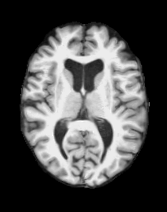
\includegraphics[width=0.5cm] {
					data/mris/control_0.png
				}
			};
			\node[draw=none, outer sep=0pt, inner sep=0pt] (i1) at \modellocation{(-3.9 * \hsep, 1.6)} {
				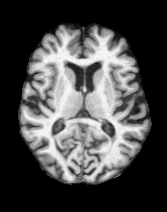
\includegraphics[width=0.5cm] {
					data/mris/control_1.png
				}
			};
			\node[draw=none, outer sep=0pt, inner sep=0pt] (i1) at \modellocation{(-4.7 * \hsep, 2.1)} {
				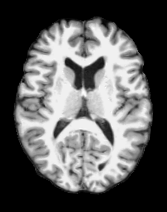
\includegraphics[width=0.5cm] {
					data/mris/control_2.png
				}
			};
			\node[draw=none, outer sep=0pt, inner sep=0pt] (i1) at \modellocation{(-4 * \hsep, 0.7)} {
				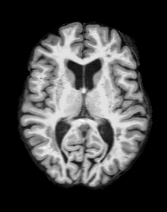
\includegraphics[width=0.5cm] {
					data/mris/control_3.png
				}
			};
			\node[draw=none, outer sep=0pt, inner sep=0pt] (i1) at \modellocation{(-5.1 * \hsep, 1.2)} {
				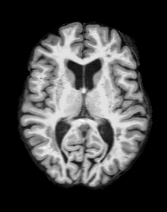
\includegraphics[width=0.5cm] {
					data/mris/control_3.png
				}
			};
			\node[align=center,font=\small\linespread{0.8}\selectfont] at \modellocation{(-4.5 * \hsep, 2.8)} {Friske\\kontroller};

			\node[draw=none, outer sep=0pt, inner sep=0pt] (i1) at \modellocation{(-4.5 * \hsep, -1.1)} {
				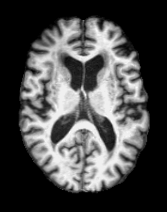
\includegraphics[width=0.5cm] {
					data/mris/dementia_0.png
				}
			};
			\node[draw=none, outer sep=0pt, inner sep=0pt] (i1) at \modellocation{(-5.1 * \hsep, -1.3)} {
				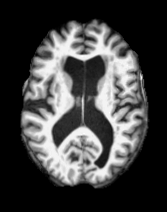
\includegraphics[width=0.5cm] {
					data/mris/dementia_1.png
				}
			};
			\node[draw=none, outer sep=0pt, inner sep=0pt] (i1) at \modellocation{(-3.9 * \hsep, -1)} {
				\includegraphics[width=0.5cm] {
					data/mris/dementia_2.png
				}
			};
			\node[draw=none, outer sep=0pt, inner sep=0pt] (i1) at \modellocation{(-4.1 * \hsep, -1.8)} {
				\includegraphics[width=0.5cm] {
					data/mris/dementia_3.png
				}
			};
			\colorlet{train-fill}{green}

			\node[align=center,font=\small\linespread{0.8}\selectfont] at \modellocation{(-4.5 * \hsep, -2.4)} {Pasienter};


			\node[circle, inner sep=0pt, fill=none, outer sep=0pt, line width=0pt, draw=none] (n00) at \modellocation{(-3 * \hsep, 0)} {};

			\node[circle, minimum size=\nodesize, inner sep=0pt, fill=train-fill!35, outer sep=0pt, line width=0pt, draw=train-fill!35] (n10) at \modellocation{(-2 * \hsep, 2 * \vsep)} {};
			\node[circle, minimum size=\nodesize, inner sep=0pt, fill=train-fill, outer sep=0pt, line width=0pt, draw=train-fill] (n11) at \modellocation{(-2 * \hsep, 1 * \vsep)} {};
			\node[circle, minimum size=\nodesize, inner sep=0pt, fill=train-fill!15, outer sep=0pt, line width=0pt, draw=train-fill!15] (n12) at \modellocation{(-2 * \hsep, 0)} {};
			\node[circle, minimum size=\nodesize, inner sep=0pt, fill=train-fill!85, outer sep=0pt, line width=0pt, draw=train-fill!85] (n13) at \modellocation{(-2 * \hsep, -1 * \vsep)} {};
			\node[circle, minimum size=\nodesize, inner sep=0pt, fill=train-fill!90, outer sep=0pt, line width=0pt, draw=train-fill!90] (n14) at \modellocation{(-2 * \hsep, -2 * \vsep)} {};

			\node[circle, minimum size=\nodesize, inner sep=0pt, fill=train-fill!55, outer sep=0pt, line width=0pt, draw=train-fill!55] (n20) at \modellocation{(-1 * \hsep, 1.5 * \vsep)} {};
			\node[circle, minimum size=\nodesize, inner sep=0pt, fill=train-fill!20, outer sep=0pt, line width=0pt, draw=train-fill!20] (n21) at \modellocation{(-1 * \hsep, 0.5 * \vsep)} {};
			\node[circle, minimum size=\nodesize, inner sep=0pt, fill=train-fill!90, outer sep=0pt, line width=0pt, draw=train-fill!50] (n22) at \modellocation{(-1 * \hsep, -0.5 * \vsep)} {};
			\node[circle, minimum size=\nodesize, inner sep=0pt, fill=train-fill!35, outer sep=0pt, line width=0pt, draw=train-fill!35] (n23) at \modellocation{(-1 * \hsep, -1.5 * \vsep)} {};

			\node[circle, minimum size=\nodesize, inner sep=0pt, fill=train-fill!95, outer sep=0pt, line width=0pt, draw=train-fill!65] (n30) at \modellocation{(0 * \hsep, 1.5 * \vsep)} {};
			\node[circle, minimum size=\nodesize, inner sep=0pt, fill=train-fill!20, outer sep=0pt, line width=0pt, draw=train-fill!20] (n31) at \modellocation{(0 * \hsep, 0.5 * \vsep)} {};
			\node[circle, minimum size=\nodesize, inner sep=0pt, fill=train-fill!90, outer sep=0pt, line width=0pt, draw=train-fill!90] (n32) at \modellocation{(0 * \hsep, -0.5 * \vsep)} {};
			\node[circle, minimum size=\nodesize, inner sep=0pt, fill=train-fill!80, outer sep=0pt, line width=0pt, draw=train-fill!80] (n33) at \modellocation{(0 * \hsep, -1.5 * \vsep)} {};

			\node[circle, minimum size=\nodesize, inner sep=0pt, fill=train-fill!50, outer sep=0pt, line width=0pt, draw=train-fill!50] (n40) at \modellocation{(1 * \hsep, 1*\vsep)} {};
			\node[circle, minimum size=\nodesize, inner sep=0pt, fill=train-fill!90, outer sep=0pt, line width=0pt, draw=train-fill!70] (n41) at \modellocation{(1 * \hsep, 0*\vsep)} {};
			\node[circle, minimum size=\nodesize, inner sep=0pt, fill=train-fill!70, outer sep=0pt, line width=0pt, draw=train-fill!30] (n42) at \modellocation{(1 * \hsep, -1*\vsep)} {};

			\node[circle, minimum size=\nodesize, inner sep=0pt, fill=train-fill, outer sep=0pt, line width=0pt, draw=train-fill] (n50) at \modellocation{(2 * \hsep, 1*\vsep)} {};
			\node[circle, minimum size=\nodesize, inner sep=0pt, fill=train-fill!70, outer sep=0pt, line width=0pt, draw=train-fill!70] (n51) at \modellocation{(2 * \hsep, 0*\vsep)} {};
			\node[circle, minimum size=\nodesize, inner sep=0pt, fill=train-fill!30, outer sep=0pt, line width=0pt, draw=train-fill!30] (n52) at \modellocation{(2 * \hsep, -1*\vsep)} {};

			\node[circle, minimum size=\nodesize, inner sep=0pt, fill=train-fill!80, outer sep=0pt, line width=0pt, draw=train-fill!65] (n60) at \modellocation{(3 * \hsep, 0)} {};

			\node[align=left, font=\linespread{0.8}\selectfont] (loss) at (0.2+2.1*4.85, -2.2) {Diagnose};

			\draw[
				color=train-fill!35,
				\innerarrow-\innerarrow,
				line width=\arrowwidth
			] (n00) to [out=20,in=200] (n10) {};
			\draw[
				color=train-fill,
				\innerarrow-\innerarrow,
				line width=\arrowwidth
			] (n00) to [out=10,in=190] (n11) {};
			\draw[
				color=train-fill!15,
				\innerarrow-\innerarrow,
				line width=\arrowwidth
			] (n00) to [out=0,in=180] (n12) {};
			\draw[
				color=train-fill!85,
				\innerarrow-\innerarrow,
				line width=\arrowwidth
			] (n00) to [out=-10,in=170] (n13) {};
			\draw[
				color=train-fill!90,
				\innerarrow-\innerarrow,
				line width=\arrowwidth
			] (n00) to [out=-20,in=160] (n14) {};

			\draw[
				color=train-fill!35,
				\innerarrow-\innerarrow,
				line width=\arrowwidth
			] (n10) to [out=-5,in=175] (n20) {};
			\draw[
				color=train-fill!10,
				\innerarrow-\innerarrow,
				line width=\arrowwidth
			] (n10) to [out=-15,in=165] (n21) {};
			\draw[
				color=train-fill!70,
				\innerarrow-\innerarrow,
				line width=\arrowwidth
			] (n10) to [out=-25,in=155] (n22) {};
			\draw[
				color=train-fill!50,
				\innerarrow-\innerarrow,
				line width=\arrowwidth
			] (n10) to [out=-35,in=145] (n23) {};

			\draw[
				color=train-fill!30,
				\innerarrow-\innerarrow,
				line width=\arrowwidth
			] (n11) to [out=5,in=185] (n20) {};
			\draw[
				color=train-fill!25,
				\innerarrow-\innerarrow,
				line width=\arrowwidth
			] (n11) to [out=-5,in=175] (n21) {};
			\draw[
				color=train-fill!95,
				\innerarrow-\innerarrow,
				line width=\arrowwidth
			] (n11) to [out=-15,in=165] (n22) {};
			\draw[
				color=train-fill!35,
				\innerarrow-\innerarrow,
				line width=\arrowwidth
			] (n11) to [out=-25,in=155] (n23) {};

			\draw[
				color=train-fill!70,
				\innerarrow-\innerarrow,
				line width=\arrowwidth
			] (n12) to [out=15,in=195] (n20) {};
			\draw[
				color=train-fill!20,
				\innerarrow-\innerarrow,
				line width=\arrowwidth
			] (n12) to [out=5,in=185] (n21) {};
			\draw[
				color=train-fill!80,
				\innerarrow-\innerarrow,
				line width=\arrowwidth
			] (n12) to [out=-5,in=175] (n22) {};
			\draw[
				color=train-fill,
				\innerarrow-\innerarrow,
				line width=\arrowwidth
			] (n12) to [out=-15,in=165] (n23) {};

			\draw[
				color=train-fill!40,
				\innerarrow-\innerarrow,
				line width=\arrowwidth
			] (n13) to [out=25,in=205] (n20) {};
			\draw[
				color=train-fill!35,
				\innerarrow-\innerarrow,
				line width=\arrowwidth
			] (n13) to [out=15,in=195] (n21) {};
			\draw[
				color=train-fill!20,
				\innerarrow-\innerarrow,
				line width=\arrowwidth
			] (n13) to [out=5,in=185] (n22) {};
			\draw[
				color=white,
				\innerarrow-\innerarrow,
				line width=\arrowwidth
			] (n13) to [out=-5,in=175] (n23) {};

			\draw[
				color=train-fill!40,
				\innerarrow-\innerarrow,
				line width=\arrowwidth
			] (n14) to [out=35,in=215] (n20) {};
			\draw[
				color=train-fill!85,
				\innerarrow-\innerarrow,
				line width=\arrowwidth
			] (n14) to [out=25,in=205] (n21) {};
			\draw[
				color=train-fill!35,
				\innerarrow-\innerarrow,
				line width=\arrowwidth
			] (n14) to [out=15,in=195] (n22) {};
			\draw[
				color=train-fill,
				\innerarrow-\innerarrow,
				line width=\arrowwidth
			] (n14) to [out=5,in=185] (n23) {};

			\draw[
				color=train-fill!85,
				\innerarrow-\innerarrow,
				line width=\arrowwidth
			] (n20) to [out=0,in=180] (n30) {};
			\draw[
				color=train-fill!50,
				\innerarrow-\innerarrow,
				line width=\arrowwidth
			] (n20) to [out=-10,in=170] (n31) {};
			\draw[
				color=train-fill!75,
				\innerarrow-\innerarrow,
				line width=\arrowwidth
			] (n20) to [out=-20,in=160] (n32) {};
			\draw[
				color=white,
				\innerarrow-\innerarrow,
				line width=\arrowwidth
			] (n20) to [out=-30,in=150] (n33) {};

			\draw[
				color=train-fill,
				\innerarrow-\innerarrow,
				line width=\arrowwidth
			] (n21) to [out=10,in=190] (n30) {};
			\draw[
				color=train-fill!30,
				\innerarrow-\innerarrow,
				line width=\arrowwidth
			] (n21) to [out=0,in=180] (n31) {};
			\draw[
				color=train-fill!25,
				\innerarrow-\innerarrow,
				line width=\arrowwidth
			] (n21) to [out=-10,in=170] (n32) {};
			\draw[
				color=white,
				\innerarrow-\innerarrow,
				line width=\arrowwidth
			] (n21) to [out=-20,in=160] (n33) {};

			\draw[
				color=train-fill!35,
				\innerarrow-\innerarrow,
				line width=\arrowwidth
			] (n22) to [out=20,in=200] (n30) {};
			\draw[
				color=train-fill!95,
				\innerarrow-\innerarrow,
				line width=\arrowwidth
			] (n22) to [out=10,in=190] (n31) {};
			\draw[
				color=train-fill!80,
				\innerarrow-\innerarrow,
				line width=\arrowwidth
			] (n22) to [out=0,in=180] (n32) {};
			\draw[
				color=white,
				\innerarrow-\innerarrow,
				line width=\arrowwidth
			] (n22) to [out=-10,in=170] (n33) {};

			\draw[
				color=train-fill!45,
				\innerarrow-\innerarrow,
				line width=\arrowwidth
			] (n23) to [out=30,in=210] (n30) {};
			\draw[
				color=train-fill!70,
				\innerarrow-\innerarrow,
				line width=\arrowwidth
			] (n23) to [out=20,in=200] (n31) {};
			\draw[
				color=train-fill!10,
				\innerarrow-\innerarrow,
				line width=\arrowwidth
			] (n23) to [out=10,in=190] (n32) {};
			\draw[
				color=train-fill!20,
				\innerarrow-\innerarrow,
				line width=\arrowwidth
			] (n23) to [out=0,in=180] (n33) {};

			\draw[
				color=train-fill!50,
				\innerarrow-\innerarrow,
				line width=\arrowwidth
			] (n30) to [out=-5,in=175] (n40) {};
			\draw[
				color=train-fill!30,
				\innerarrow-\innerarrow,
				line width=\arrowwidth
			] (n30) to [out=-15,in=165] (n41) {};
			\draw[
				color=train-fill,
				\innerarrow-\innerarrow,
				line width=\arrowwidth
			] (n30) to [out=-25,in=155] (n42) {};

			\draw[
				color=train-fill!45,
				\innerarrow-\innerarrow,
				line width=\arrowwidth
			] (n31) to [out=5,in=185] (n40) {};
			\draw[
				color=train-fill!90,
				-\innerarrow,
				line width=\arrowwidth
			] (n31) to [out=-5,in=175] (n41) {};
			\draw[
				color=train-fill!45,
				\innerarrow-\innerarrow,
				line width=\arrowwidth
			] (n31) to [out=-15,in=165] (n42) {};

			\draw[
				color=train-fill!15,
				\innerarrow-\innerarrow,
				line width=\arrowwidth
			] (n32) to [out=15,in=195] (n40) {};
			\draw[
				color=train-fill!70,
				\innerarrow-\innerarrow,
				line width=\arrowwidth
			] (n32) to [out=5,in=185] (n41) {};
			\draw[
				color=train-fill!50,
				\innerarrow-\innerarrow,
				line width=\arrowwidth
			] (n32) to [out=-5,in=175] (n42) {};

			\draw[
				color=train-fill!40,
				\innerarrow-\innerarrow,
				line width=\arrowwidth
			] (n33) to [out=25,in=205] (n40) {};
			\draw[
				color=train-fill!20,
				\innerarrow-\innerarrow,
				line width=\arrowwidth
			] (n33) to [out=15,in=195] (n41) {};
			\draw[
				color=train-fill!90,
				\innerarrow-\innerarrow,
				line width=\arrowwidth
			] (n33) to [out=5,in=185] (n42) {};

			\draw[
				color=train-fill!25,
				\innerarrow-\innerarrow,
				line width=\arrowwidth
			] (n40) to [out=0,in=180] (n50) {};
			\draw[
				color=train-fill!15,
				-\innerarrow,
				line width=\arrowwidth
			] (n40) to [out=-10,in=170] (n51) {};
			\draw[
				color=train-fill,
				\innerarrow-\innerarrow,
				line width=\arrowwidth
			] (n40) to [out=-20,in=160] (n52) {};

			\draw[
				color=train-fill!35,
				\innerarrow-\innerarrow,
				line width=\arrowwidth
			] (n41) to [out=10,in=190] (n50) {};
			\draw[
				color=train-fill!10,
				\innerarrow-\innerarrow,
				line width=\arrowwidth
			] (n41) to [out=0,in=180] (n51) {};
			\draw[
				color=train-fill!90,
				\innerarrow-\innerarrow,
				line width=\arrowwidth
			] (n41) to [out=-10,in=170] (n52) {};

			\draw[
				color=train-fill!50,
				\innerarrow-\innerarrow,
				line width=\arrowwidth
			] (n42) to [out=20,in=200] (n50) {};
			\draw[
				color=train-fill!40,
				\innerarrow-\innerarrow,
				line width=\arrowwidth
			] (n42) to [out=10,in=190] (n51) {};
			\draw[
				color=train-fill!20,
				\innerarrow-\innerarrow,
				line width=\arrowwidth
			] (n42) to [out=0,in=180] (n52) {};

			\draw[
				color=train-fill!80,
				\innerarrow-\innerarrow,
				line width=\arrowwidth,
			] (n50) to [out=-10,in=170] (n60) {};
			\draw[
				color=train-fill!90,
				\innerarrow-\innerarrow,
				line width=\arrowwidth,
			] (n51) to [out=0,in=180] (n60) {};
			\draw[
				color=train-fill!30,
				\innerarrow-\innerarrow,
				line width=\arrowwidth,
			] (n52) to [out=10,in=190] (n60) {};

			\draw[black] (n00.center) --
							($ (n00) + (0, 2*\vsep+0.5*\nodesize+2pt) $) --
							($ (n00) + (6*\hsep+0.5*\nodesize+2pt, 2*\vsep+0.5*\nodesize+2pt) $) --
							($ (n00) + (6*\hsep+0.5*\nodesize+2pt, -2*\vsep-0.5*\nodesize-2pt) $) --
							($ (n00) + (0, -2*\vsep-0.5*\nodesize-2pt) $) --
							(n00.center);

			\node[] at ($ (n30) + (0, \vsep+0.5*\nodesize) $) {Konvolusjonelt nevralt nett};

			\draw[
				color=outercolor,
				-\outerarrow,
				line width=0.1cm
			] \modellocation{(-4.5 * \hsep, -0.6)} to [out=90,in=180] (n00) {};

			\draw[
				color=outercolor,
				-\outerarrow,
				line width=0.1cm
			] \modellocation{(-4.5 * \hsep, 0.6)} to [out=270,in=180] (n00) {};

			\draw[
				color=outercolor,
				-\outerarrow,
				line width=0.1cm
			] (n60) to [out=0,in=180] (loss) {};

			\node[] at (0.6, 1.5) {};
			\node[] at (11, -5.5) {};
		\end{tikzpicture}
	\end{frame}

	\begin{frame}[b]{AI i hjerneforskning: Diagnostisk klassifisering} % Alzheimer
		\centering
		\begin{tikzpicture}
			\begin{axis}[
				xmode=log,
				xlabel={Antall scans},
				ylabel=Treffsikkerhet,
				ytick={80, 85, 90, 95},
				yticklabels={80\%, 85\%, 90\%, 95\%},
				xtick={100, 1000, 10000},
				xticklabels={100, 1000, 10000}
			]
				\addplot[only marks,fill=teal!40] coordinates {
					(1805,89.8)
					(518,88.5)
					(60,88)
					(149,91)
					(16455,87)
					(388,84.4)
					(510,85)
					(319,85.5)
					(60,86.8)
					(23,95.7)
					(577,90.7)
					(386,88.8)
					(197,82.7)
					(346,92.5)
					(1116,86.1)
					(716,87)
					(60,95)
					(636,89.5)
					(821,90.3)
					(83,88)
					(40,90)
					(575,92.3)
					(69,92.1)
					(176,94.2)
					(83,96.8)
					(382,93.2)
					(102,79.2)
					(565,85.2)
					(200,88)
					(200,90)
					(46,92.5)
					(467,95.8)
					(469,90.7)
					(258,91.3)
					(258,90.0)
					(258,89.2)
				};
			\end{axis}
		\end{tikzpicture}\\
		\vspace{1cm}
		Klassifisering av Alzheimer's sykdom\\
	\end{frame}

	\begin{frame}{AI i hjerneforskning: Diagnostisk klassifisering} % Psychiatric
		\centering
		\begin{tikzpicture}
			\node[inner sep=0pt, draw=black] {
				\includegraphics[width=8cm]{data/psychiatric.jpg}
			};
		\end{tikzpicture}
	\end{frame}

	\begin{frame}{AI i hjerneforskning: Diagnostisk klassifisering} % Summary
		\noindent Hvorfor er diagnostisk klassifisering i mange tilfeller lite hensiktsmessig?
		\begin{itemize}
			\item Forutsetter at pasientene allerede er syke.
			\item Forutsetter at vi allerede vet at pasientene er syke.
			\item Forutsetter at det finnes en vel-definert pasient-gruppe.
			\item Vi har en god klassifikator. Hva nå?
		\end{itemize}
	\end{frame}

	\begin{frame}{AI i hjerneforskning: Hjernealder} % Outline
		\centering
		\vfill
		\begin{tikzpicture}
			\node[
				inner sep=0pt,
				outer sep=0pt,
				draw=black,
				fill=white,
			] at (0, 0) {
				\includegraphics[width=7cm]{data/cole.jpg}
			};
		\end{tikzpicture}
		\vfill
	\end{frame}

	\setbeamertemplate{footline}[deep]

	\begin{frame}{AI i hjerneforskning: Hjernealder} % Datasett
		\definecolor{hbn-clr}{RGB}{255, 0, 40}
		\definecolor{adhd200-clr}{RGB}{255, 27, 0}
		\definecolor{ping-clr}{RGB}{255, 96, 0}
		\definecolor{ds000119-clr}{RGB}{255, 165, 0}
		\definecolor{abide-clr}{RGB}{255, 234, 0}
		\definecolor{slim-clr}{RGB}{206, 255, 0}
		\definecolor{abide2-clr}{RGB}{137, 255, 0}
		\definecolor{beijing-clr}{RGB}{68, 255, 0}
		\definecolor{aomic-clr}{RGB}{0, 255, 0}
		\definecolor{corr-clr}{RGB}{0, 255, 68}
		\definecolor{mpi-clr}{RGB}{0, 255, 137}
		\definecolor{hcp-clr}{RGB}{0, 255, 205}
		\definecolor{fcon-clr}{RGB}{0, 235, 255}
		\definecolor{nki-clr}{RGB}{0, 166, 255}
		\definecolor{sald-clr}{RGB}{0, 97, 255}
		\definecolor{ds000222-clr}{RGB}{0, 27, 255}
		\definecolor{dlbs-clr}{RGB}{41, 0, 255}
		\definecolor{camcan-clr}{RGB}{110, 0, 255}
		\definecolor{ukb-clr}{RGB}{180, 0, 255}
		\definecolor{oasis-clr}{RGB}{249, 0, 255}
		\definecolor{ds000202-clr}{RGB}{255, 0, 191}

		\centering
		\vfill
		\begin{tikzpicture}
			\begin{axis}[
				width=0.9\textwidth,
				height=0.65\textwidth,
				xmin=0,
				xmax=100,
				ymin=-1200,
				ymax=1200,
				yticklabels={,,},
				ytick=\empty,
				xtick pos=bottom,
				y dir=reverse,
				axis x line=middle,
				axis y line=none,
				xtick={0,10,20,30,40,50,60,70,80}
			]
				\addplot [draw=none, name path=zero] coordinates {
					(0, 0)
					(100, 0)
				};

				\addplot [draw=none, name path=hbn] table [col sep=comma, x=age,y=hbn] {data/paper1/dataset/M.csv};
				\addplot [hbn-clr] fill between [of=zero and hbn];
				\addplot [draw=none, name path=adhd200] table [col sep=comma, x=age,y=adhd200-hc] {data/paper1/dataset/M.csv};
				\addplot [adhd200-clr] fill between [of=hbn and adhd200];\label{trace:adhd200}
				\addplot [draw=none, name path=ping] table [col sep=comma, x=age,y=ping] {data/paper1/dataset/M.csv};
				\addplot [ping-clr] fill between [of=adhd200 and ping];\label{trace:ping}

				\addplot [draw=none, name path=ds000119] table [col sep=comma, x=age,y=ds000119] {data/paper1/dataset/M.csv};
				\addplot [ds000119-clr] fill between [of=ping and ds000119];\label{trace:ds000119}
				\addplot [draw=none, name path=abide] table [col sep=comma, x=age,y=abide-hc] {data/paper1/dataset/M.csv};
				\addplot [abide-clr] fill between [of=ds000119 and abide];\label{trace:abide}
				\addplot [draw=none, name path=slim] table [col sep=comma, x=age,y=slim] {data/paper1/dataset/M.csv};
				\addplot [slim-clr] fill between [of=abide and slim];\label{trace:slim}
				\addplot [draw=none, name path=abide2] table [col sep=comma, x=age,y=abide2-hc] {data/paper1/dataset/M.csv};
				\addplot [abide2-clr] fill between [of=slim and abide2];\label{trace:abide2}
				\addplot [draw=none, name path=beijing] table [col sep=comma, x=age,y=beijing-enhanced] {data/paper1/dataset/M.csv};
				\addplot [beijing-clr] fill between [of=slim and beijing];\label{trace:beijing}
				\addplot [draw=none, name path=aomic] table [col sep=comma, x=age,y=aomic-id1000] {data/paper1/dataset/M.csv};
				\addplot [aomic-clr] fill between [of=beijing and aomic];\label{trace:aomic}
				\addplot [draw=none, name path=corr] table [col sep=comma, x=age,y=corr] {data/paper1/dataset/M.csv};
				\addplot [corr-clr] fill between [of=aomic and corr];\label{trace:corr}
				\addplot [draw=none, name path=mpi] table [col sep=comma, x=age,y=mpi-lemon] {data/paper1/dataset/M.csv};
				\addplot [mpi-clr] fill between [of=corr and mpi];\label{trace:mpi}
				\addplot [draw=none, name path=hcp] table [col sep=comma, x=age,y=hcp] {data/paper1/dataset/M.csv};
				\addplot [hcp-clr] fill between [of=mpi and hcp];\label{trace:hcp}
				\addplot [draw=none, name path=fcon] table [col sep=comma, x=age,y=fcon1000] {data/paper1/dataset/M.csv};
				\addplot [fcon-clr] fill between [of=hcp and fcon];\label{trace:fcon}
				\addplot [draw=none, name path=nki] table [col sep=comma, x=age,y=nki-rockland] {data/paper1/dataset/M.csv};
				\addplot [nki-clr] fill between [of=fcon and nki];\label{trace:nki}
				\addplot [draw=none, name path=sald] table [col sep=comma, x=age,y=sald] {data/paper1/dataset/M.csv};
				\addplot [sald-clr] fill between [of=nki and sald];\label{trace:sald}
				\addplot [draw=none, name path=ds000222] table [col sep=comma, x=age,y=ds000222] {data/paper1/dataset/M.csv};
				\addplot [ds000222-clr] fill between [of=sald and ds000222];\label{trace:ds000222}
				\addplot [draw=none, name path=dlbs] table [col sep=comma, x=age,y=dlbs] {data/paper1/dataset/M.csv};
				\addplot [dlbs-clr] fill between [of=ds000222 and dlbs];\label{trace:dlbs}
				\addplot [draw=none, name path=camcan] table [col sep=comma, x=age,y=camcan] {data/paper1/dataset/M.csv};
				\addplot [camcan-clr] fill between [of=dlbs and camcan];\label{trace:camcan}
				\addplot [draw=none, name path=ukb] table [col sep=comma, x=age,y=ukb] {data/paper1/dataset/M.csv};
				\addplot [ukb-clr] fill between [of=camcan and ukb];\label{trace:ukb}
				\addplot [draw=black, name path=oasis] table [col sep=comma, x=age,y=oasis3-hc] {data/paper1/dataset/M.csv};
				\addplot [oasis-clr] fill between [of=ukb and oasis];\label{trace:oasis}

				\addplot [draw=none, name path=hbn] table [col sep=comma, x=age,y expr=\thisrow{hbn}*-1] {data/paper1/dataset/F.csv};
				\addplot [hbn-clr] fill between [of=zero and hbn];\label{trace:hbn}
				\addplot [draw=none, name path=adhd200] table [col sep=comma, x=age,y=,y expr=\thisrow{adhd200-hc}*-1] {data/paper1/dataset/F.csv};
				\addplot [adhd200-clr] fill between [of=hbn and adhd200];
				\addplot [draw=none, name path=ping] table [col sep=comma, x=age,y expr=\thisrow{ping}*-1] {data/paper1/dataset/F.csv};
				\addplot [ping-clr] fill between [of=adhd200 and ping];
				\addplot [draw=none, name path=abide] table [col sep=comma, x=age,y expr=\thisrow{abide-hc}*-1] {data/paper1/dataset/F.csv};
				\addplot [abide-clr] fill between [of=ping and abide];
				\addplot [draw=none, name path=abide2] table [col sep=comma, x=age,y expr=\thisrow{abide2-hc}*-1] {data/paper1/dataset/F.csv};
				\addplot [abide2-clr] fill between [of=abide and abide2];
				\addplot [draw=none, name path=ds000119] table [col sep=comma, x=age,y=,y expr=\thisrow{ds000119}*-1] {data/paper1/dataset/F.csv};
				\addplot [ds000119-clr] fill between [of=abide2 and ds000119];
				\addplot [draw=none, name path=slim] table [col sep=comma, x=age,y expr=\thisrow{slim}*-1] {data/paper1/dataset/F.csv};
				\addplot [slim-clr] fill between [of=ds000119 and slim];
				\addplot [draw=none, name path=beijing] table [col sep=comma, x=age,y expr=\thisrow{beijing-enhanced}*-1] {data/paper1/dataset/F.csv};
				\addplot [beijing-clr] fill between [of=slim and beijing];
				\addplot [draw=none, name path=ds000202] table [col sep=comma, x=age,y expr=\thisrow{ds000202}*-1] {data/paper1/dataset/F.csv};
				\addplot [ds000202-clr] fill between [of=beijing and ds000202];\label{trace:ds000202}
				\addplot [draw=none, name path=aomic] table [col sep=comma, x=age,y expr=\thisrow{aomic-id1000}*-1] {data/paper1/dataset/F.csv};
				\addplot [aomic-clr] fill between [of=beijing and aomic];
				\addplot [draw=none, name path=mpi] table [col sep=comma, x=age,y expr=\thisrow{mpi-lemon}*-1] {data/paper1/dataset/F.csv};
				\addplot [mpi-clr] fill between [of=aomic and mpi];
				\addplot [draw=none, name path=corr] table [col sep=comma, x=age,y expr=\thisrow{corr}*-1] {data/paper1/dataset/F.csv};
				\addplot [corr-clr] fill between [of=mpi and corr];
				\addplot [draw=none, name path=fcon] table [col sep=comma, x=age,y expr=\thisrow{fcon1000}*-1] {data/paper1/dataset/F.csv};
				\addplot [fcon-clr] fill between [of=corr and fcon];
				\addplot [draw=none, name path=hcp] table [col sep=comma, x=age, y expr=\thisrow{hcp}*-1] {data/paper1/dataset/F.csv};
				\addplot [hcp-clr] fill between [of=fcon and hcp];
				\addplot [draw=none, name path=nki] table [col sep=comma, x=age,y expr=\thisrow{nki-rockland}*-1] {data/paper1/dataset/F.csv};
				\addplot [nki-clr] fill between [of=hcp and nki];
				\addplot [draw=none, name path=ds000222] table [col sep=comma, x=age,y expr=\thisrow{ds000222}*-1] {data/paper1/dataset/F.csv};
				\addplot [ds000222-clr] fill between [of=nki and ds000222];
				\addplot [draw=none, name path=sald] table [col sep=comma, x=age,y expr=\thisrow{sald}*-1] {data/paper1/dataset/F.csv};
				\addplot [sald-clr] fill between [of=ds000222 and sald];
				\addplot [draw=none, name path=camcan] table [col sep=comma, x=age,y expr=\thisrow{camcan}*-1] {data/paper1/dataset/F.csv};
				\addplot [camcan-clr] fill between [of=sald and camcan];
				\addplot [draw=none, name path=dlbs] table [col sep=comma, x=age,y expr=\thisrow{dlbs}*-1] {data/paper1/dataset/F.csv};
				\addplot [dlbs-clr] fill between [of=camcan and dlbs];

				\addplot [draw=none, name path=ukb] table [col sep=comma, x=age,y expr=\thisrow{ukb}*-1] {data/paper1/dataset/F.csv};
				\addplot [ukb-clr] fill between [of=dlbs and ukb];
				\addplot [draw=black, name path=oasis] table [col sep=comma, x=age,y expr=\thisrow{oasis3-hc}*-1] {data/paper1/dataset/F.csv};
				\addplot [oasis-clr] fill between [of=ukb and oasis];

				\addplot [] coordinates {
					(0, 0)
					(100, 0)
				};
				\coordinate (male) at (axis cs:100,35) {};
				\coordinate (female) at (axis cs:100,-35) {};

				\node[] at (50,220) {\textbf{n=53,542}};
			\end{axis}
			\matrix [
				draw=none,
				matrix of nodes,
				anchor=north west,
				row sep=-0.1cm,
				font=\footnotesize,
				column 1/.style={anchor=base west}
			] at (8.2, 6.31) {
				\ref{trace:hbn} HBN \\
				\ref{trace:adhd200} ADHD200 \\
				\ref{trace:ping} PING \\
				\ref{trace:ds000119} ds000119 \\
				\ref{trace:abide} ABIDE \\
				\ref{trace:slim} SLIM \\
				\ref{trace:abide2} ABIDE2 \\
				\ref{trace:beijing} Beijing \\
				\ref{trace:aomic} AOMIC \\
				\ref{trace:corr} CoRR \\
				\ref{trace:mpi} MPI-Lemon \\
				\ref{trace:hcp} HCP \\
				\ref{trace:fcon} FCON1000 \\
				\ref{trace:nki} NKI Rockland \\
				\ref{trace:sald} SALD \\
				\ref{trace:ds000222} ds000222 \\
				\ref{trace:dlbs} DLBS \\
				\ref{trace:camcan} CamCAN \\
				\ref{trace:ukb} UKB \\
				\ref{trace:oasis} OASIS3 \\
				\ref{trace:ds000202} ds000202 \\
			};
			\node [anchor=north east] at (male) {\footnotesize{MENN}};
			\node [anchor=south east] at (female) {\footnotesize{KVINNER}};
		\end{tikzpicture}
		\vfill
	\end{frame}

	\begin{frame}{AI i hjerneforskning: Hjernealder} % Modelling
        \centering
        \vfill
		\begin{tikzpicture}[scale=0.9]
            \newcommand{\mrivsep}{0.52}
			\newcommand{\mrihsep}{0.44}
			\def\plotwidth{11.68}

			\newcommand{\nodesize}{11pt}
			\newcommand{\hsep}{28pt}
			\newcommand{\vsep}{14pt}

			\newcommand{\arrowwidth}{0.05cm}
			\newcommand{\innerarrow}{{Latex[length=0.1cm, width=0.15cm]}}
			\newcommand{\outerarrow}{{Latex[length=0.2cm, width=0.3cm]}}

			\definecolor{cb-green}{HTML}{4dac93}
			\definecolor{cb-blue}{HTML}{3594d6}
			\definecolor{outercolor}{RGB}{128, 128, 128}
			\colorlet{train-fill}{cb-blue}

			\newcommand{\patientlocation}[1]{($ (1, -1.6) + ####1 $)}
			\newcommand{\controllocation}[1]{($ (1, -2.8) + ####1 $)}
			\newcommand{\modellocation}[1]{($ (0.5 * \plotwidth, -2.2) + ####1 $)}

			\node[draw=none, outer sep=0pt, inner sep=0pt] (input) at \modellocation{(-5 * \hsep, 0)} {
				\includegraphics[width=1.5cm] {
					data/mris/control_0.png
				}
			};

			\node[circle, inner sep=0pt, fill=none, outer sep=0pt, line width=0pt, draw=none] (n00) at \modellocation{(-3 * \hsep, 0)} {};

			\node[circle, minimum size=\nodesize, inner sep=0pt, fill=train-fill!35, outer sep=0pt, line width=0pt, draw=train-fill!35] (n10) at \modellocation{(-2 * \hsep, 2 * \vsep)} {};
			\node[circle, minimum size=\nodesize, inner sep=0pt, fill=train-fill, outer sep=0pt, line width=0pt, draw=train-fill] (n11) at \modellocation{(-2 * \hsep, 1 * \vsep)} {};
			\node[circle, minimum size=\nodesize, inner sep=0pt, fill=train-fill!15, outer sep=0pt, line width=0pt, draw=train-fill!15] (n12) at \modellocation{(-2 * \hsep, 0)} {};
			\node[circle, minimum size=\nodesize, inner sep=0pt, fill=train-fill!85, outer sep=0pt, line width=0pt, draw=train-fill!85] (n13) at \modellocation{(-2 * \hsep, -1 * \vsep)} {};
			\node[circle, minimum size=\nodesize, inner sep=0pt, fill=train-fill!90, outer sep=0pt, line width=0pt, draw=train-fill!90] (n14) at \modellocation{(-2 * \hsep, -2 * \vsep)} {};

			\node[circle, minimum size=\nodesize, inner sep=0pt, fill=train-fill!55, outer sep=0pt, line width=0pt, draw=train-fill!55] (n20) at \modellocation{(-1 * \hsep, 1.5 * \vsep)} {};
			\node[circle, minimum size=\nodesize, inner sep=0pt, fill=train-fill!20, outer sep=0pt, line width=0pt, draw=train-fill!20] (n21) at \modellocation{(-1 * \hsep, 0.5 * \vsep)} {};
			\node[circle, minimum size=\nodesize, inner sep=0pt, fill=train-fill!90, outer sep=0pt, line width=0pt, draw=train-fill!50] (n22) at \modellocation{(-1 * \hsep, -0.5 * \vsep)} {};
			\node[circle, minimum size=\nodesize, inner sep=0pt, fill=train-fill!35, outer sep=0pt, line width=0pt, draw=train-fill!35] (n23) at \modellocation{(-1 * \hsep, -1.5 * \vsep)} {};

			\node[circle, minimum size=\nodesize, inner sep=0pt, fill=train-fill!95, outer sep=0pt, line width=0pt, draw=train-fill!65] (n30) at \modellocation{(0 * \hsep, 1.5 * \vsep)} {};
			\node[circle, minimum size=\nodesize, inner sep=0pt, fill=train-fill!20, outer sep=0pt, line width=0pt, draw=train-fill!20] (n31) at \modellocation{(0 * \hsep, 0.5 * \vsep)} {};
			\node[circle, minimum size=\nodesize, inner sep=0pt, fill=train-fill!90, outer sep=0pt, line width=0pt, draw=train-fill!90] (n32) at \modellocation{(0 * \hsep, -0.5 * \vsep)} {};
			\node[circle, minimum size=\nodesize, inner sep=0pt, fill=train-fill!80, outer sep=0pt, line width=0pt, draw=train-fill!80] (n33) at \modellocation{(0 * \hsep, -1.5 * \vsep)} {};

			\node[circle, minimum size=\nodesize, inner sep=0pt, fill=train-fill!50, outer sep=0pt, line width=0pt, draw=train-fill!50] (n40) at \modellocation{(1 * \hsep, 1*\vsep)} {};
			\node[circle, minimum size=\nodesize, inner sep=0pt, fill=train-fill!90, outer sep=0pt, line width=0pt, draw=train-fill!70] (n41) at \modellocation{(1 * \hsep, 0*\vsep)} {};
			\node[circle, minimum size=\nodesize, inner sep=0pt, fill=train-fill!70, outer sep=0pt, line width=0pt, draw=train-fill!30] (n42) at \modellocation{(1 * \hsep, -1*\vsep)} {};

			\node[circle, minimum size=\nodesize, inner sep=0pt, fill=train-fill, outer sep=0pt, line width=0pt, draw=train-fill] (n50) at \modellocation{(2 * \hsep, 1*\vsep)} {};
			\node[circle, minimum size=\nodesize, inner sep=0pt, fill=train-fill!70, outer sep=0pt, line width=0pt, draw=train-fill!70] (n51) at \modellocation{(2 * \hsep, 0*\vsep)} {};
			\node[circle, minimum size=\nodesize, inner sep=0pt, fill=train-fill!30, outer sep=0pt, line width=0pt, draw=train-fill!30] (n52) at \modellocation{(2 * \hsep, -1*\vsep)} {};

			\node[circle, minimum size=\nodesize, inner sep=0pt, fill=train-fill!80, outer sep=0pt, line width=0pt, draw=train-fill!65] (n60) at \modellocation{(3 * \hsep, 0)} {};

			\node[align=left, font=\linespread{0.8}\selectfont] (loss) at (0.5+2.1*4.85, -2.2) {Predikert\\hjernealder};

			\draw[
				color=train-fill!35,
				-\innerarrow,
				line width=\arrowwidth
			] (n00) to [out=20,in=200] (n10) {};
			\draw[
				color=train-fill,
				-\innerarrow,
				line width=\arrowwidth
			] (n00) to [out=10,in=190] (n11) {};
			\draw[
				color=train-fill!15,
				-\innerarrow,
				line width=\arrowwidth
			] (n00) to [out=0,in=180] (n12) {};
			\draw[
				color=train-fill!85,
				-\innerarrow,
				line width=\arrowwidth
			] (n00) to [out=-10,in=170] (n13) {};
			\draw[
				color=train-fill!90,
				-\innerarrow,
				line width=\arrowwidth
			] (n00) to [out=-20,in=160] (n14) {};

			\draw[
				color=train-fill!35,
				-\innerarrow,
				line width=\arrowwidth
			] (n10) to [out=-5,in=175] (n20) {};
			\draw[
				color=train-fill!10,
				-\innerarrow,
				line width=\arrowwidth
			] (n10) to [out=-15,in=165] (n21) {};
			\draw[
				color=train-fill!70,
				-\innerarrow,
				line width=\arrowwidth
			] (n10) to [out=-25,in=155] (n22) {};
			\draw[
				color=train-fill!50,
				-\innerarrow,
				line width=\arrowwidth
			] (n10) to [out=-35,in=145] (n23) {};

			\draw[
				color=train-fill!30,
				-\innerarrow,
				line width=\arrowwidth
			] (n11) to [out=5,in=185] (n20) {};
			\draw[
				color=train-fill!25,
				-\innerarrow,
				line width=\arrowwidth
			] (n11) to [out=-5,in=175] (n21) {};
			\draw[
				color=train-fill!95,
				-\innerarrow,
				line width=\arrowwidth
			] (n11) to [out=-15,in=165] (n22) {};
			\draw[
				color=train-fill!35,
				-\innerarrow,
				line width=\arrowwidth
			] (n11) to [out=-25,in=155] (n23) {};

			\draw[
				color=train-fill!70,
				-\innerarrow,
				line width=\arrowwidth
			] (n12) to [out=15,in=195] (n20) {};
			\draw[
				color=train-fill!20,
				-\innerarrow,
				line width=\arrowwidth
			] (n12) to [out=5,in=185] (n21) {};
			\draw[
				color=train-fill!80,
				-\innerarrow,
				line width=\arrowwidth
			] (n12) to [out=-5,in=175] (n22) {};
			\draw[
				color=train-fill,
				-\innerarrow,
				line width=\arrowwidth
			] (n12) to [out=-15,in=165] (n23) {};

			\draw[
				color=train-fill!40,
				-\innerarrow,
				line width=\arrowwidth
			] (n13) to [out=25,in=205] (n20) {};
			\draw[
				color=train-fill!35,
				-\innerarrow,
				line width=\arrowwidth
			] (n13) to [out=15,in=195] (n21) {};
			\draw[
				color=train-fill!20,
				-\innerarrow,
				line width=\arrowwidth
			] (n13) to [out=5,in=185] (n22) {};
			\draw[
				color=white,
				-\innerarrow,
				line width=\arrowwidth
			] (n13) to [out=-5,in=175] (n23) {};

			\draw[
				color=train-fill!40,
				-\innerarrow,
				line width=\arrowwidth
			] (n14) to [out=35,in=215] (n20) {};
			\draw[
				color=train-fill!85,
				-\innerarrow,
				line width=\arrowwidth
			] (n14) to [out=25,in=205] (n21) {};
			\draw[
				color=train-fill!35,
				-\innerarrow,
				line width=\arrowwidth
			] (n14) to [out=15,in=195] (n22) {};
			\draw[
				color=train-fill,
				-\innerarrow,
				line width=\arrowwidth
			] (n14) to [out=5,in=185] (n23) {};

			\draw[
				color=train-fill!85,
				-\innerarrow,
				line width=\arrowwidth
			] (n20) to [out=0,in=180] (n30) {};
			\draw[
				color=train-fill!50,
				-\innerarrow,
				line width=\arrowwidth
			] (n20) to [out=-10,in=170] (n31) {};
			\draw[
				color=train-fill!75,
				-\innerarrow,
				line width=\arrowwidth
			] (n20) to [out=-20,in=160] (n32) {};
			\draw[
				color=white,
				-\innerarrow,
				line width=\arrowwidth
			] (n20) to [out=-30,in=150] (n33) {};

			\draw[
				color=train-fill,
				-\innerarrow,
				line width=\arrowwidth
			] (n21) to [out=10,in=190] (n30) {};
			\draw[
				color=train-fill!30,
				-\innerarrow,
				line width=\arrowwidth
			] (n21) to [out=0,in=180] (n31) {};
			\draw[
				color=train-fill!25,
				-\innerarrow,
				line width=\arrowwidth
			] (n21) to [out=-10,in=170] (n32) {};
			\draw[
				color=white,
				-\innerarrow,
				line width=\arrowwidth
			] (n21) to [out=-20,in=160] (n33) {};

			\draw[
				color=train-fill!35,
				-\innerarrow,
				line width=\arrowwidth
			] (n22) to [out=20,in=200] (n30) {};
			\draw[
				color=train-fill!95,
				-\innerarrow,
				line width=\arrowwidth
			] (n22) to [out=10,in=190] (n31) {};
			\draw[
				color=train-fill!80,
				-\innerarrow,
				line width=\arrowwidth
			] (n22) to [out=0,in=180] (n32) {};
			\draw[
				color=white,
				-\innerarrow,
				line width=\arrowwidth
			] (n22) to [out=-10,in=170] (n33) {};

			\draw[
				color=train-fill!45,
				-\innerarrow,
				line width=\arrowwidth
			] (n23) to [out=30,in=210] (n30) {};
			\draw[
				color=train-fill!70,
				-\innerarrow,
				line width=\arrowwidth
			] (n23) to [out=20,in=200] (n31) {};
			\draw[
				color=train-fill!10,
				-\innerarrow,
				line width=\arrowwidth
			] (n23) to [out=10,in=190] (n32) {};
			\draw[
				color=train-fill!20,
				-\innerarrow,
				line width=\arrowwidth
			] (n23) to [out=0,in=180] (n33) {};

			\draw[
				color=train-fill!50,
				-\innerarrow,
				line width=\arrowwidth
			] (n30) to [out=-5,in=175] (n40) {};
			\draw[
				color=train-fill!30,
				-\innerarrow,
				line width=\arrowwidth
			] (n30) to [out=-15,in=165] (n41) {};
			\draw[
				color=train-fill,
				-\innerarrow,
				line width=\arrowwidth
			] (n30) to [out=-25,in=155] (n42) {};

			\draw[
				color=train-fill!45,
				-\innerarrow,
				line width=\arrowwidth
			] (n31) to [out=5,in=185] (n40) {};
			\draw[
				color=train-fill!90,
				-\innerarrow,
				line width=\arrowwidth
			] (n31) to [out=-5,in=175] (n41) {};
			\draw[
				color=train-fill!45,
				-\innerarrow,
				line width=\arrowwidth
			] (n31) to [out=-15,in=165] (n42) {};

			\draw[
				color=train-fill!15,
				-\innerarrow,
				line width=\arrowwidth
			] (n32) to [out=15,in=195] (n40) {};
			\draw[
				color=train-fill!70,
				-\innerarrow,
				line width=\arrowwidth
			] (n32) to [out=5,in=185] (n41) {};
			\draw[
				color=train-fill!50,
				-\innerarrow,
				line width=\arrowwidth
			] (n32) to [out=-5,in=175] (n42) {};

			\draw[
				color=train-fill!40,
				-\innerarrow,
				line width=\arrowwidth
			] (n33) to [out=25,in=205] (n40) {};
			\draw[
				color=train-fill!20,
				-\innerarrow,
				line width=\arrowwidth
			] (n33) to [out=15,in=195] (n41) {};
			\draw[
				color=train-fill!90,
				-\innerarrow,
				line width=\arrowwidth
			] (n33) to [out=5,in=185] (n42) {};

			\draw[
				color=train-fill!25,
				-\innerarrow,
				line width=\arrowwidth
			] (n40) to [out=0,in=180] (n50) {};
			\draw[
				color=train-fill!15,
				-\innerarrow,
				line width=\arrowwidth
			] (n40) to [out=-10,in=170] (n51) {};
			\draw[
				color=train-fill,
				-\innerarrow,
				line width=\arrowwidth
			] (n40) to [out=-20,in=160] (n52) {};

			\draw[
				color=train-fill!35,
				-\innerarrow,
				line width=\arrowwidth
			] (n41) to [out=10,in=190] (n50) {};
			\draw[
				color=train-fill!10,
				-\innerarrow,
				line width=\arrowwidth
			] (n41) to [out=0,in=180] (n51) {};
			\draw[
				color=train-fill!90,
				-\innerarrow,
				line width=\arrowwidth
			] (n41) to [out=-10,in=170] (n52) {};

			\draw[
				color=train-fill!50,
				-\innerarrow,
				line width=\arrowwidth
			] (n42) to [out=20,in=200] (n50) {};
			\draw[
				color=train-fill!40,
				-\innerarrow,
				line width=\arrowwidth
			] (n42) to [out=10,in=190] (n51) {};
			\draw[
				color=train-fill!20,
				-\innerarrow,
				line width=\arrowwidth
			] (n42) to [out=0,in=180] (n52) {};

			\draw[
				color=train-fill!80,
				-\innerarrow,
				line width=\arrowwidth,
			] (n50) to [out=-10,in=170] (n60) {};
			\draw[
				color=train-fill!90,
				-\innerarrow,
				line width=\arrowwidth,
			] (n51) to [out=0,in=180] (n60) {};
			\draw[
				color=train-fill!30,
				-\innerarrow,
				line width=\arrowwidth,
			] (n52) to [out=10,in=190] (n60) {};

			\draw[black] (n00.center) --
							($ (n00) + (0, 2*\vsep+0.5*\nodesize+2pt) $) --
							($ (n00) + (6*\hsep+0.5*\nodesize+2pt, 2*\vsep+0.5*\nodesize+2pt) $) --
							($ (n00) + (6*\hsep+0.5*\nodesize+2pt, -2*\vsep-0.5*\nodesize-2pt) $) --
							($ (n00) + (0, -2*\vsep-0.5*\nodesize-2pt) $) --
							(n00.center);

			\node[] at ($ (n30) + (0, \vsep+0.5*\nodesize) $) {Konvolusjonelt nevralt nett};

			\draw[
				color=outercolor,
				-\outerarrow,
				line width=0.1cm
			] (input) to [out=0,in=180] (n00) {};
			\draw[
				color=outercolor,
				-\outerarrow,
				line width=0.1cm
			] (n60) to [out=0,in=180] (loss) {};
		\end{tikzpicture}
        \vfill
	\end{frame}

	\begin{frame}{AI i hjerneforskning: Hjernealder} % Accuracy
		\def\N{1}
		\centering
		\vfill
		\begin{tikzpicture}
			\begin{groupplot}[
				group style={
					group size=2 by 1,
					horizontal sep=1.2cm,
					vertical sep=0.8cm
				},
				width=0.5\linewidth,
				height=0.5\linewidth
			]

				\nextgroupplot[
					xmin=0,
					xmax=100,
					ymin=0,
					ymax=100,
					xtick pos=bottom,
					ytick pos=left,
					ticklabel style = {font=\footnotesize},
					xlabel={Kronologisk alder},
					ylabel={Predikert hjernealder},
					title={Testsett}
				]
					\addplot [red] coordinates {(0,0) (100,100)};
					\addplot [
						only marks,
						mark size=1.5pt,
						color=black,
						opacity=0.35
					] table [
						x=regression,
						y=age,
						each nth point={\N},
						col sep=comma
					] {data/paper1/prediction/test_predictions.csv};
					\node [anchor=south east,inner sep=0pt,outer sep=0pt] (outofsample) at (rel axis cs:0.92,0.08) {\textcolor{red}{MAE=2.47}};

				\nextgroupplot[
					xmin=0,
					xmax=100,
					ymin=0,
					ymax=100,
					xtick pos=bottom,
					ytick pos=left,
					ticklabel style = {font=\footnotesize},
					title={Eksternt testsett}
				]
					\addplot [red] coordinates {(0,0) (100,100)};
					\addplot [
						only marks,
						mark size=1.5pt,
						color=black,
						opacity=0.35
					] table [
						x=regression,
						y=age,
						each nth point={\N},
						col sep=comma
					] {data/paper1/prediction/external_predictions.csv};
					\node [anchor=south east,inner sep=0pt,outer sep=0pt] (outofsample) at (rel axis cs:0.92,0.08) {\textcolor{red}{MAE=3.90}};
			\end{groupplot}
	  \end{tikzpicture}
	  \vfill
	\end{frame}

	\begin{frame}{AI i hjerneforskning: Hjernealder} % Associations
		\definecolor{pwas}{HTML}{70F3FF}
		\definecolor{neg}{HTML}{AAFF99}
		\definecolor{pos}{HTML}{FF8585}
		\definecolor{bars}{HTML}{A899FF}

        \centering
        \vfill

  		\begin{columns}[T]
    		\column{0.6\textwidth}
				\begin{tikzpicture}
					\begin{axis}[
							width=1.15\textwidth,
							height=\textwidth,
							ylabel=$-\mathrm{log}_{10}(p)$,
							y label style={at={(-0.06, 0.5)}},
							ymin=0,
							ymax=11.5,
							xmin=-1,
							xmax=395,
							ytick={2,4,6,8,10},
							yticklabels={-2,-4,-6,-8,-10},
							axis x line*=bottom,
							axis y line=left,
							xtick={32.5,102.5,149.5,177.5,208.5,
								233,254.5,275.5,301.5,334.5,
								358,372,388},
							xticklabels={1,2,3,4,5,6,7,8,9,10,
										11,12,13},
							tick label style={font=\scriptsize},
							clip=false,
							xlabel={Kategorier}
						]
						\addplot[draw=black, only marks, mark size=1.5pt, fill=pwas] table [x=x,y=y,col sep=comma] {data/pwas.csv};
						\addplot[draw=black,dashed] coordinates {(-1, 3.896) (395, 3.896)};
						\addplot[draw=black,dotted] coordinates {(65,0) (65,11.5)};
						\addplot[draw=black,dotted] coordinates {(140,0) (140,11.5)};
						\addplot[draw=black,dotted] coordinates {(159,0) (159,11.5)};
						\addplot[draw=black,dotted] coordinates {(196,0) (196,11.5)};
						\addplot[draw=black,dotted] coordinates {(221,0) (221,11.5)};
						\addplot[draw=black,dotted] coordinates {(245,0) (245,11.5)};
						\addplot[draw=black,dotted] coordinates {(264,0) (264,11.5)};
						\addplot[draw=black,dotted] coordinates {(287,0) (287,11.5)};
						\addplot[draw=black,dotted] coordinates {(316,0) (316,11.5)};
						\addplot[draw=black,dotted] coordinates {(353,0) (353,11.5)};
						\addplot[draw=black,dotted] coordinates {(363,0) (363,11.5)};
						\addplot[draw=black,dotted] coordinates {(381,0) (381,11.5)};
						\addplot[draw=black,dotted] coordinates {(395,0) (395,11.5)};
						\node[anchor=south] at (axis cs:12,6.09) {\tiny{HbA1c}};
						\node[anchor=south] at (axis cs:18,10.49) {\tiny{Glucose}};
						\node[anchor=north] at (axis cs:26,10.23) {\tiny{IGF-1}};
						\node[anchor=south] at (axis cs:49,4.47) {\tiny{Corpuscular volume}};
						\node[anchor=south, align=center] at (axis cs:65,6.72) {\tiny{Vascular/heart}\\[-1.5ex] \tiny{problem}};
						\node[anchor=south, align=center] at (axis cs:89,9.93) {\tiny{Blood pressure}\\[-1.5ex] \tiny{medication}};
						\node[anchor=south] at (axis cs:128,6.64) {\tiny{Diabetes}};
						\node[anchor=south] at (axis cs:254,6.94) {\tiny{Weekly beer/cider intake}};
						\node[anchor=south, align=center] at (axis cs:303,4.61) {\tiny{Total cigarette}\\[-1.5ex] \tiny{packs}};
						\node[anchor=south, align=center] at (axis cs:376,5.33) {\tiny{Non-UK country}\\[-1.5ex] \tiny{of birth}};
					\end{axis}
				\end{tikzpicture}

			\column{0.4\textwidth} % Adjust the width of the second column
				%\vspace*{-0.35cm}
				\begin{tikzpicture}
					\begin{groupplot}[
						group style={
									group size=2 by 1,
									horizontal sep=2cm
								},
								width=0.6\textwidth,
								height=1.5\textwidth,
						]
						\nextgroupplot[
							yticklabels={,,},
							xmin=-1,
							xmax=0,
							xtick={0, -0.5, -1},
							ymin=0,
							ymax=19,
							axis x line=bottom,
							axis y line*=right,
							x axis line style={stealth-},
							ymajorticks=false,
							tick label style={font=\scriptsize}
						]
							\addplot[fill=neg] coordinates {
								(0,0.1)
								(0,0.9)
								(-0.627,0.9)
								(-0.627,0.1)
								(0,0.1)
							};

							\addplot[fill=neg] coordinates {
								(0,1.1)
								(0,1.9)
								(-0.272,1.9)
								(-0.272,1.1)
								(0,1.1)
							};

							\addplot[fill=neg] coordinates {
								(0,2.1)
								(0,2.9)
								(-0.225,2.9)
								(-0.225,2.1)
								(0,2.1)
							};

							\addplot[fill=neg] coordinates {
								(0,3.1)
								(0,3.9)
								(-0.166,3.9)
								(-0.166,3.1)
								(0,3.1)
							};

							\addplot[fill=neg] coordinates {
								(0,4.1)
								(0,4.9)
								(-0.136,4.9)
								(-0.136,4.1)
								(0,4.1)
							};

							\coordinate (1) at (axis cs: 0.99,0.5) {};
							\coordinate (2) at (axis cs: 0.99,1.5) {};
							\coordinate (3) at (axis cs: 0.99,2.5) {};
							\coordinate (4) at (axis cs: 0.99,3.5) {};
							\coordinate (5) at (axis cs: 0.99,4.5) {};
							\coordinate (6) at (axis cs: 0.99,5.5) {};
							\coordinate (7) at (axis cs: 0.99,6.5) {};
							\coordinate (8) at (axis cs: 0.99,7.5) {};
							\coordinate (9) at (axis cs: 0.99,8.5) {};
							\coordinate (10) at (axis cs: 0.99,9.5) {};
							\coordinate (11) at (axis cs: 0.99,10.5) {};
							\coordinate (12) at (axis cs: 0.99,11.5) {};
							\coordinate (13) at (axis cs: 0.99,12.5) {};
							\coordinate (14) at (axis cs: 0.99,13.5) {};
							\coordinate (15) at (axis cs: 0.99,14.5) {};
							\coordinate (16) at (axis cs: 0.99,15.5) {};
							\coordinate (17) at (axis cs: 0.99,16.5) {};
							\coordinate (18) at (axis cs: 0.99,17.5) {};
							\coordinate (19) at (axis cs: 0.99,18.5) {};
						\nextgroupplot[
							yticklabels={,,},
							xmin=0,
							xmax=2,
							ymin=0,
							ymax=19,
							axis x line=bottom,
							axis y line*=left,
							ymajorticks=false,,
							tick label style={font=\scriptsize}
						]

							\addplot[fill=pos] coordinates {
								(0,5.1)
								(0,5.9)
								(0.127,5.9)
								(0.127,5.1)
								(0,5.1)
							};

							\addplot[fill=pos] coordinates {
								(0,6.1)
								(0,6.9)
								(0.137,6.9)
								(0.137,6.1)
								(0,6.1)
							};

							\addplot[fill=pos] coordinates {
								(0,7.1)
								(0,7.9)
								(0.156,7.9)
								(0.156,7.1)
								(0,7.1)
							};

							\addplot[fill=pos] coordinates {
								(0,8.1)
								(0,8.9)
								(0.161,8.9)
								(0.161,8.1)
								(0,8.1)
							};

							\addplot[fill=pos] coordinates {
								(0,9.1)
								(0,9.9)
								(0.169,9.9)
								(0.169,9.1)
								(0,9.1)
							};

							\addplot[fill=pos] coordinates {
								(0,10.1)
								(0,10.9)
								(0.211,10.9)
								(0.211,10.1)
								(0,10.1)
							};

							\addplot[fill=pos] coordinates {
								(0,11.1)
								(0,11.9)
								(0.230,11.9)
								(0.230,11.1)
								(0,11.1)
							};

							\addplot[fill=pos] coordinates {
								(0,12.1)
								(0,12.9)
								(0.246,12.9)
								(0.246,12.1)
								(0,12.1)
							};

							\addplot[fill=pos] coordinates {
								(0,13.1)
								(0,13.9)
								(0.251,13.9)
								(0.251,13.1)
								(0,13.1)
							};

							\addplot[fill=pos] coordinates {
								(0,14.1)
								(0,14.9)
								(0.265,14.9)
								(0.265,14.1)
								(0,14.1)
							};

							\addplot[fill=pos] coordinates {
								(0,15.1)
								(0,15.9)
								(0.415,15.9)
								(0.415,15.1)
								(0,15.1)
							};

							\addplot[fill=pos] coordinates {
								(0,16.1)
								(0,16.9)
								(0.540,16.9)
								(0.540,16.1)
								(0,16.1)
							};

							\addplot[fill=pos] coordinates {
								(0,17.1)
								(0,17.9)
								(0.74,17.9)
								(0.74,17.1)
								(0,17.1)
							};

							\addplot[fill=pos] coordinates {
								(0,18.1)
								(0,18.9)
								(1.786,18.9)
								(1.786,18.1)
								(0,18.1)
							};

					\end{groupplot}
					\node [align=center] at ($ (1) - (0, 0.6) $) {Effektstørrelser};
					\node [align=center,font=\tiny\linespread{0.8}\selectfont] at (1) {Non-UK country of birth};
					\node [align=center,font=\tiny\linespread{0.8}\selectfont] at (2) {Other group activity};
					\node [align=center,font=\tiny\linespread{0.8}\selectfont] at (3) {IGF-1};
					\node [align=center,font=\tiny\linespread{0.8}\selectfont] at (4) {Cereal intake};
					\node [align=center,font=\tiny\linespread{0.8}\selectfont] at (5) {Number in household};
					\node [align=center,font=\tiny\linespread{0.8}\selectfont] at (6) {Alcohol intake freq.};
					\node [align=center,font=\tiny\linespread{0.8}\selectfont] at (7) {Corpuscular volume};
					\node [align=center,font=\tiny\linespread{0.8}\selectfont] at (8) {Diastolic BP};
					\node [align=center,font=\tiny\linespread{0.8}\selectfont] at (9) {Systolic BP};
					\node [align=center,font=\tiny\linespread{0.8}\selectfont] at (10) {HbA1c};
					\node [align=center,font=\tiny\linespread{0.8}\selectfont] at (11) {Weekly beer/cider intake};
					\node [align=center,font=\tiny\linespread{0.8}\selectfont] at (12) {Glucose};
					\node [align=center,font=\tiny\linespread{0.8}\selectfont] at (13) {Total cigarette packs};
					\node [align=center,font=\tiny\linespread{0.8}\selectfont] at (14) {Age stopped smoking};
					\node [align=center,font=\tiny\linespread{0.8}\selectfont] at (15) {Cigarette packs per year};
					\node [align=center,font=\tiny\linespread{0.8}\selectfont] at (16) {Vascular/heart problem};
					\node [align=center,font=\tiny\linespread{0.8}\selectfont] at (17) {BP medication};
					\node [align=center,font=\tiny\linespread{0.8}\selectfont] at (18) {Diabetes};
					\node [align=center,font=\tiny\linespread{0.8}\selectfont] at (19) {Diabetic retinopathy};
        		\end{tikzpicture}
		\end{columns}
		\vfill
	\end{frame}

	\begin{frame}{AI i hjerneforskning: Hjernealder} % Patient cohorts
        \centering
        \vfill
		\begin{figure}
			\begin{center}
				\begin{tikzpicture}
					\begin{axis}[
						height=0.7\textwidth,
						width=0.7\textwidth,
						axis x line=bottom,
						hide y axis,
						xmin=-19,
						xmax=19,
						ymin=-0.1,
						ymax=6.6,
						xlabel=Hjernealdergap,
						axis line style={latex-latex}
					]
						\addplot [black, dashed] coordinates {(0,-0.3) (0,9)};

						\addplot [blue,very thick,name path=MScontrols] table [x=x,y expr=\thisrow{control} + 5.5,col sep=comma] {data/paper1/supplementary/MS/delta_distributions.csv};
						\addplot [red,very thick,name path=MSpatients] table [x=x,y expr=\thisrow{patient} + 5.5,col sep=comma] {data/paper1/supplementary/MS/delta_distributions.csv};
						\addplot [draw=none,name path=MSbaseline] coordinates {(-20,5.5) (20,5.5)};
						\addplot [blue,fill opacity=0.3] fill between [of=MScontrols and MSbaseline];
						\addplot [red,fill opacity=0.3] fill between [of=MSpatients and MSbaseline];
						\coordinate (MS) at (axis cs:19,6.7) {};
						\addplot [blue,very thick,name path=ADcontrols] table [x=x,y expr=\thisrow{control} + 4.4,col sep=comma] {data/paper1/supplementary/AD/delta_distributions.csv};
						\addplot [red,very thick,name path=ADpatients] table [x=x,y expr=\thisrow{patient} + 4.4,col sep=comma] {data/paper1/supplementary/AD/delta_distributions.csv};
						\addplot [draw=none,name path=ADbaseline] coordinates {(-20,4.4) (20,4.4)};
						\addplot [blue,fill opacity=0.3] fill between [of=ADcontrols and ADbaseline];
						\addplot [red,fill opacity=0.3] fill between [of=ADpatients and ADbaseline];
						\coordinate (AD) at (axis cs:19,5.6) {};
						\addplot [blue,very thick,name path=MCIcontrols] table [x=x,y expr=\thisrow{control} + 3.3,col sep=comma] {data/paper1/supplementary/MCI/delta_distributions.csv};
						\addplot [red,very thick,name path=MCIpatients] table [x=x,y expr=\thisrow{patient} + 3.3,col sep=comma] {data/paper1/supplementary/MCI/delta_distributions.csv};
						\addplot [draw=none,name path=MCIbaseline] coordinates {(-20,3.3) (20,3.3)};
						\addplot [blue,fill opacity=0.3] fill between [of=MCIcontrols and MCIbaseline];
						\addplot [red,fill opacity=0.3] fill between [of=MCIpatients and MCIbaseline];
						\coordinate (MCI) at (axis cs:19,4.5) {};
						\addplot [blue,very thick,name path=SCZcontrols] table [x=x,y expr=\thisrow{control} + 2.2,col sep=comma] {data/paper1/supplementary/SCZ/delta_distributions.csv};
						\addplot [red,very thick,name path=SCZpatients] table [x=x,y expr=\thisrow{patient} + 2.2,col sep=comma] {data/paper1/supplementary/SCZ/delta_distributions.csv};
						\addplot [draw=none,name path=SCZbaseline] coordinates {(-20,2.2) (20,2.2)};
						\addplot [blue,fill opacity=0.3] fill between [of=SCZcontrols and SCZbaseline];
						\addplot [red,fill opacity=0.3] fill between [of=SCZpatients and SCZbaseline];
						\coordinate (SCZ) at (axis cs:19,3.4) {};
						\addplot [blue,very thick,name path=PSYcontrols] table [x=x,y expr=\thisrow{control} + 1.1,col sep=comma] {data/paper1/supplementary/PSY/delta_distributions.csv};
						\addplot [red,very thick,name path=PSYpatients] table [x=x,y expr=\thisrow{patient} + 1.1,col sep=comma] {data/paper1/supplementary/PSY/delta_distributions.csv};
						\addplot [draw=none,name path=PSYbaseline] coordinates {(-20,1.1) (20,1.1)};
						\addplot [blue,fill opacity=0.3] fill between [of=PSYcontrols and PSYbaseline];
						\addplot [red,fill opacity=0.3] fill between [of=PSYpatients and PSYbaseline];
						\coordinate (PSY) at (axis cs:19,2.3) {};
						\addplot [blue,very thick,name path=MOODcontrols] table [x=x,y expr=\thisrow{control},col sep=comma] {data/paper1/supplementary/MOOD/delta_distributions.csv};
						\addplot [red,very thick,name path=MOODpatients] table [x=x,y expr=\thisrow{patient},col sep=comma] {data/paper1/supplementary/MOOD/delta_distributions.csv};
						\addplot [draw=none,name path=MOODbaseline] coordinates {(-20,0) (20,0)};
						\addplot [blue,fill opacity=0.3] fill between [of=MOODcontrols and MOODbaseline];
						\addplot [red,fill opacity=0.3] fill between [of=MOODpatients and MOODbaseline];
						\coordinate (MOOD) at (axis cs:19,1.2) {};
					\end{axis}
					\matrix [
						matrix of nodes,
						draw=none,
						row sep=-0.15cm,
						anchor=north west,
						column 1/.style={anchor=base west, nodes={font=\tiny}}
					] at (MS) {
						\textbf{\underline{MS}} \\
						$\Delta=4.42$\\
						$p=1.71*10^{-22}$\\
						$d=0.87$\\
					};
					\matrix [
						matrix of nodes,
						draw=none,
						row sep=-0.15cm,
						anchor=north west,
						column 1/.style={anchor=base west, nodes={font=\tiny}}
					] at (AD) {
						\textbf{\underline{AD}} \\
						$\Delta=2.81$\\
						$p=4.27*10^{-20}$\\
						$d=0.58$\\
					};
					\matrix [
						matrix of nodes,
						draw=none,
						row sep=-0.15cm,
						anchor=north west,
						column 1/.style={anchor=base west, nodes={font=\tiny}}
					] at (MCI) {
						\textbf{\underline{MCI}} \\
						$\Delta=2.13$\\
						$p=1.25*10^{-15}$\\
						$d=0.46$\\
					};
					\matrix [
						matrix of nodes,
						draw=none,
						row sep=-0.15cm,
						anchor=north west,
						column 1/.style={anchor=base west, nodes={font=\tiny}}
					] at (SCZ) {
						\textbf{\underline{SCZ}} \\
						$\Delta=1.40$\\
						$p=4.29*10^{-5}$\\
						$d=0.34$\\
					};
					\matrix [
						matrix of nodes,
						draw=none,
						row sep=-0.15cm,
						anchor=north west,
						column 1/.style={anchor=base west, nodes={font=\tiny}}
					] at (PSY) {
						\textbf{\underline{PSY}} \\
						$\Delta=0.74$\\
						$p=0.15$\textcolor{white}{$5^2$}\\
						$d=0.20$\\
					};
					\matrix [
						matrix of nodes,
						draw=none,
						row sep=-0.15cm,
						anchor=north west,
						column 1/.style={anchor=base west, nodes={font=\tiny}}
					] at (MOOD) {
						\textbf{\underline{MOOD}} \\
						$\Delta=0.64$\\
						$p=0.04$\textcolor{white}{$5^2$}\\
						$d=0.17$\\
					};

				\end{tikzpicture}
			\end{center}
		\end{figure}
        \vfill
	\end{frame}

	\begin{frame}{AI i hjerneforskning: Hjernealder} % Summary
		Hjernealder er et potensielt data-derivert mål på hjernens generelle helse
		\begin{itemize}
			\item[\textcolor{green}+] Oppsummerer all informasjonen i en hjernescan i ett tall.
			\item[\textcolor{green}+] Intuitivt.
			\item[\textcolor{green}+] Samvarierer med andre faktorer (hjerteproblemer, alkoholinntak, røyking).
			\item[\textcolor{green}+] Varierer mellom sykdomsgrupper (multippel sklerose, Alzheimer's sykdom).
			\item[\textcolor{red}-] Ikke et direkte mål på helsetilstand.
			\item[\textcolor{red}-] Usikkert hvordan det skal tolkes.
			\item[\textcolor{red}-] Hva er det modellen ser på?
		\end{itemize}
	\end{frame}

	\definecolor{train-fill}{HTML}{0079FF}

	\begin{frame}{AI i hjerneforskning: Forklarbar AI} % ANNs
		\begin{tikzpicture}
			\newcommand{\nodesize}{8pt}
			\newcommand{\hsep}{24pt}
			\newcommand{\vsep}{12pt}

			\newcommand{\arrowwidth}{0.05cm}
			\newcommand{\innerarrow}{{Latex[length=0.1cm, width=0.15cm]}}

			\newcommand{\modellocation}[1]{($ (0, 0) + ####1 $)}

			\node[circle, inner sep=0pt, fill=none, outer sep=0pt, line width=0pt, draw=none] (n00) at \modellocation{(-3 * \hsep, 0)} {};
			\node[] at (-5.5, 1.5) {};
			\node[] at (5.1, -1.2) {};

			\draw[black, fill=gray!20] (n00.center) --
							($ (n00) + (0, 2*\vsep+0.5*\nodesize+2pt) $) --
							($ (n00) + (6*\hsep+0.5*\nodesize+2pt, 2*\vsep+0.5*\nodesize+2pt) $) --
							($ (n00) + (6*\hsep+0.5*\nodesize+2pt, -2*\vsep-0.5*\nodesize-2pt) $) --
							($ (n00) + (0, -2*\vsep-0.5*\nodesize-2pt) $) --
							(n00.center);


			\node[circle, draw=black, minimum size=\nodesize, inner sep=0pt, fill=gray, outer sep=0pt, line width=0pt, draw=gray] (n10) at \modellocation{(-2 * \hsep, 2 * \vsep)} {};
			\node[circle, minimum size=\nodesize, inner sep=0pt, fill=gray, outer sep=0pt, line width=0pt, draw=gray] (n11) at \modellocation{(-2 * \hsep, 1 * \vsep)} {};
			\node[circle, minimum size=\nodesize, inner sep=0pt, fill=gray, outer sep=0pt, line width=0pt, draw=gray] (n12) at \modellocation{(-2 * \hsep, 0)} {};
			\node[circle, minimum size=\nodesize, inner sep=0pt, fill=gray, outer sep=0pt, line width=0pt, draw=gray] (n13) at \modellocation{(-2 * \hsep, -1 * \vsep)} {};
			\node[circle, minimum size=\nodesize, inner sep=0pt, fill=gray, outer sep=0pt, line width=0pt, draw=gray] (n14) at \modellocation{(-2 * \hsep, -2 * \vsep)} {};

			\node[circle, minimum size=\nodesize, inner sep=0pt, fill=gray, outer sep=0pt, line width=0pt, draw=gray] (n20) at \modellocation{(-1 * \hsep, 1.5 * \vsep)} {};
			\node[circle, minimum size=\nodesize, inner sep=0pt, fill=gray, outer sep=0pt, line width=0pt, draw=gray] (n21) at \modellocation{(-1 * \hsep, 0.5 * \vsep)} {};
			\node[circle, minimum size=\nodesize, inner sep=0pt, fill=gray, outer sep=0pt, line width=0pt, draw=gray] (n22) at \modellocation{(-1 * \hsep, -0.5 * \vsep)} {};
			\node[circle, minimum size=\nodesize, inner sep=0pt, fill=gray, outer sep=0pt, line width=0pt, draw=gray] (n23) at \modellocation{(-1 * \hsep, -1.5 * \vsep)} {};

			\node[circle, minimum size=\nodesize, inner sep=0pt, fill=gray, outer sep=0pt, line width=0pt, draw=gray] (n30) at \modellocation{(0 * \hsep, 1.5 * \vsep)} {};
			\node[circle, minimum size=\nodesize, inner sep=0pt, fill=gray, outer sep=0pt, line width=0pt, draw=gray] (n31) at \modellocation{(0 * \hsep, 0.5 * \vsep)} {};
			\node[circle, minimum size=\nodesize, inner sep=0pt, fill=gray, outer sep=0pt, line width=0pt, draw=gray] (n32) at \modellocation{(0 * \hsep, -0.5 * \vsep)} {};
			\node[circle, minimum size=\nodesize, inner sep=0pt, fill=gray, outer sep=0pt, line width=0pt, draw=gray] (n33) at \modellocation{(0 * \hsep, -1.5 * \vsep)} {};

			\node[circle, minimum size=\nodesize, inner sep=0pt, fill=gray, outer sep=0pt, line width=0pt, draw=gray] (n40) at \modellocation{(1 * \hsep, 1*\vsep)} {};
			\node[circle, minimum size=\nodesize, inner sep=0pt, fill=gray, outer sep=0pt, line width=0pt, draw=gray] (n41) at \modellocation{(1 * \hsep, 0*\vsep)} {};
			\node[circle, minimum size=\nodesize, inner sep=0pt, fill=gray, outer sep=0pt, line width=0pt, draw=gray] (n42) at \modellocation{(1 * \hsep, -1*\vsep)} {};

			\node[circle, minimum size=\nodesize, inner sep=0pt, fill=gray, outer sep=0pt, line width=0pt, draw=gray] (n50) at \modellocation{(2 * \hsep, 1*\vsep)} {};
			\node[circle, minimum size=\nodesize, inner sep=0pt, fill=gray, outer sep=0pt, line width=0pt, draw=gray] (n51) at \modellocation{(2 * \hsep, 0*\vsep)} {};
			\node[circle, minimum size=\nodesize, inner sep=0pt, fill=gray, outer sep=0pt, line width=0pt, draw=gray] (n52) at \modellocation{(2 * \hsep, -1*\vsep)} {};

			\node[circle, minimum size=\nodesize, inner sep=0pt, fill=gray, outer sep=0pt, line width=0pt, draw=gray] (n60) at \modellocation{(3 * \hsep, 0)} {};

			\draw[
				color=gray!70,
				-\innerarrow,
				line width=\arrowwidth
			] (n00) to [out=20,in=200] (n10) {};
			\draw[
				color=gray!70,
				-\innerarrow,
				line width=\arrowwidth
			] (n00) to [out=10,in=190] (n11) {};
			\draw[
				color=gray!70,
				-\innerarrow,
				line width=\arrowwidth
			] (n00) to [out=0,in=180] (n12) {};
			\draw[
				color=gray!70,
				-\innerarrow,
				line width=\arrowwidth
			] (n00) to [out=-10,in=170] (n13) {};
			\draw[
				color=gray!70,
				-\innerarrow,
				line width=\arrowwidth
			] (n00) to [out=-20,in=160] (n14) {};

			\draw[
				color=gray!70,
				-\innerarrow,
				line width=\arrowwidth
			] (n10) to [out=-5,in=175] (n20) {};
			\draw[
				color=gray!70,
				-\innerarrow,
				line width=\arrowwidth
			] (n10) to [out=-15,in=165] (n21) {};
			\draw[
				color=gray!70,
				-\innerarrow,
				line width=\arrowwidth
			] (n10) to [out=-25,in=155] (n22) {};
			\draw[
				color=gray!70,
				-\innerarrow,
				line width=\arrowwidth
			] (n10) to [out=-35,in=145] (n23) {};

			\draw[
				color=gray!70,
				-\innerarrow,
				line width=\arrowwidth
			] (n11) to [out=5,in=185] (n20) {};
			\draw[
				color=gray!70,
				-\innerarrow,
				line width=\arrowwidth
			] (n11) to [out=-5,in=175] (n21) {};
			\draw[
				color=gray!70,
				-\innerarrow,
				line width=\arrowwidth
			] (n11) to [out=-15,in=165] (n22) {};
			\draw[
				color=gray!70,
				-\innerarrow,
				line width=\arrowwidth
			] (n11) to [out=-25,in=155] (n23) {};

			\draw[
				color=gray!70,
				-\innerarrow,
				line width=\arrowwidth
			] (n12) to [out=15,in=195] (n20) {};
			\draw[
				color=gray!70,
				-\innerarrow,
				line width=\arrowwidth
			] (n12) to [out=5,in=185] (n21) {};
			\draw[
				color=gray!70,
				-\innerarrow,
				line width=\arrowwidth
			] (n12) to [out=-5,in=175] (n22) {};
			\draw[
				color=gray!70,
				-\innerarrow,
				line width=\arrowwidth
			] (n12) to [out=-15,in=165] (n23) {};

			\draw[
				color=gray!70,
				-\innerarrow,
				line width=\arrowwidth
			] (n13) to [out=25,in=205] (n20) {};
			\draw[
				color=gray!70,
				-\innerarrow,
				line width=\arrowwidth
			] (n13) to [out=15,in=195] (n21) {};
			\draw[
				color=gray!70,
				-\innerarrow,
				line width=\arrowwidth
			] (n13) to [out=5,in=185] (n22) {};
			\draw[
				color=gray!70,
				-\innerarrow,
				line width=\arrowwidth
			] (n13) to [out=-5,in=175] (n23) {};

			\draw[
				color=gray!70,
				-\innerarrow,
				line width=\arrowwidth
			] (n14) to [out=35,in=215] (n20) {};
			\draw[
				color=gray!70,
				-\innerarrow,
				line width=\arrowwidth
			] (n14) to [out=25,in=205] (n21) {};
			\draw[
				color=gray!70,
				-\innerarrow,
				line width=\arrowwidth
			] (n14) to [out=15,in=195] (n22) {};
			\draw[
				color=gray!70,
				-\innerarrow,
				line width=\arrowwidth
			] (n14) to [out=5,in=185] (n23) {};

			\draw[
				color=gray!70,
				-\innerarrow,
				line width=\arrowwidth
			] (n20) to [out=0,in=180] (n30) {};
			\draw[
				color=gray!70,
				-\innerarrow,
				line width=\arrowwidth
			] (n20) to [out=-10,in=170] (n31) {};
			\draw[
				color=gray!70,
				-\innerarrow,
				line width=\arrowwidth
			] (n20) to [out=-20,in=160] (n32) {};
			\draw[
				color=gray!70,
				-\innerarrow,
				line width=\arrowwidth
			] (n20) to [out=-30,in=150] (n33) {};

			\draw[
				color=gray!70,
				-\innerarrow,
				line width=\arrowwidth
			] (n21) to [out=10,in=190] (n30) {};
			\draw[
				color=gray!70,
				-\innerarrow,
				line width=\arrowwidth
			] (n21) to [out=0,in=180] (n31) {};
			\draw[
				color=gray!70,
				-\innerarrow,
				line width=\arrowwidth
			] (n21) to [out=-10,in=170] (n32) {};
			\draw[
				color=gray!70,
				-\innerarrow,
				line width=\arrowwidth
			] (n21) to [out=-20,in=160] (n33) {};

			\draw[
				color=gray!70,
				-\innerarrow,
				line width=\arrowwidth
			] (n22) to [out=20,in=200] (n30) {};
			\draw[
				color=gray!70,
				-\innerarrow,
				line width=\arrowwidth
			] (n22) to [out=10,in=190] (n31) {};
			\draw[
				color=gray!70,
				-\innerarrow,
				line width=\arrowwidth
			] (n22) to [out=0,in=180] (n32) {};
			\draw[
				color=gray!70,
				-\innerarrow,
				line width=\arrowwidth
			] (n22) to [out=-10,in=170] (n33) {};

			\draw[
				color=gray!70,
				-\innerarrow,
				line width=\arrowwidth
			] (n23) to [out=30,in=210] (n30) {};
			\draw[
				color=gray!70,
				-\innerarrow,
				line width=\arrowwidth
			] (n23) to [out=20,in=200] (n31) {};
			\draw[
				color=gray!70,
				-\innerarrow,
				line width=\arrowwidth
			] (n23) to [out=10,in=190] (n32) {};
			\draw[
				color=gray!70,
				-\innerarrow,
				line width=\arrowwidth
			] (n23) to [out=0,in=180] (n33) {};

			\draw[
				color=gray!70,
				-\innerarrow,
				line width=\arrowwidth
			] (n30) to [out=-5,in=175] (n40) {};
			\draw[
				color=gray!70,
				-\innerarrow,
				line width=\arrowwidth
			] (n30) to [out=-15,in=165] (n41) {};
			\draw[
				color=gray!70,
				-\innerarrow,
				line width=\arrowwidth
			] (n30) to [out=-25,in=155] (n42) {};

			\draw[
				color=gray!70,
				-\innerarrow,
				line width=\arrowwidth
			] (n31) to [out=5,in=185] (n40) {};
			\draw[
				color=gray!70,
				-\innerarrow,
				line width=\arrowwidth
			] (n31) to [out=-5,in=175] (n41) {};
			\draw[
				color=gray!70,
				-\innerarrow,
				line width=\arrowwidth
			] (n31) to [out=-15,in=165] (n42) {};

			\draw[
				color=gray!70,
				-\innerarrow,
				line width=\arrowwidth
			] (n32) to [out=15,in=195] (n40) {};
			\draw[
				color=gray!70,
				-\innerarrow,
				line width=\arrowwidth
			] (n32) to [out=5,in=185] (n41) {};
			\draw[
				color=gray!70,
				-\innerarrow,
				line width=\arrowwidth
			] (n32) to [out=-5,in=175] (n42) {};

			\draw[
				color=gray!70,
				-\innerarrow,
				line width=\arrowwidth
			] (n33) to [out=25,in=205] (n40) {};
			\draw[
				color=gray!70,
				-\innerarrow,
				line width=\arrowwidth
			] (n33) to [out=15,in=195] (n41) {};
			\draw[
				color=gray!70,
				-\innerarrow,
				line width=\arrowwidth
			] (n33) to [out=5,in=185] (n42) {};

			\draw[
				color=gray!70,
				-\innerarrow,
				line width=\arrowwidth
			] (n40) to [out=0,in=180] (n50) {};
			\draw[
				color=gray!70,
				-\innerarrow,
				line width=\arrowwidth
			] (n40) to [out=-10,in=170] (n51) {};
			\draw[
				color=gray!70,
				-\innerarrow,
				line width=\arrowwidth
			] (n40) to [out=-20,in=160] (n52) {};

			\draw[
				color=gray!70,
				-\innerarrow,
				line width=\arrowwidth
			] (n41) to [out=10,in=190] (n50) {};
			\draw[
				color=gray!70,
				-\innerarrow,
				line width=\arrowwidth
			] (n41) to [out=0,in=180] (n51) {};
			\draw[
				color=gray!70,
				-\innerarrow,
				line width=\arrowwidth
			] (n41) to [out=-10,in=170] (n52) {};

			\draw[
				color=gray!70,
				-\innerarrow,
				line width=\arrowwidth
			] (n42) to [out=20,in=200] (n50) {};
			\draw[
				color=gray!70,
				-\innerarrow,
				line width=\arrowwidth
			] (n42) to [out=10,in=190] (n51) {};
			\draw[
				color=gray!70,
				-\innerarrow,
				line width=\arrowwidth
			] (n42) to [out=0,in=180] (n52) {};

			\draw[
				color=gray!70,
				-\innerarrow,
				line width=\arrowwidth,
			] (n50) to [out=-10,in=170] (n60) {};
			\draw[
				color=gray!70,
				-\innerarrow,
				line width=\arrowwidth,
			] (n51) to [out=0,in=180] (n60) {};
			\draw[
				color=gray!70,
				-\innerarrow,
				line width=\arrowwidth,
			] (n52) to [out=10,in=190] (n60) {};


			\node[] at ($ (n30) + (0, \vsep+0.75*\nodesize) $) {Konvolusjonelt nevralt nettverk};
		\end{tikzpicture}
	\end{frame}

	\begin{frame}{AI i hjerneforskning: Forklarbar AI} % Input
		\begin{tikzpicture}
			\newcommand{\nodesize}{8pt}
			\newcommand{\hsep}{24pt}
			\newcommand{\vsep}{12pt}

			\newcommand{\arrowwidth}{0.05cm}
			\newcommand{\innerarrow}{{Latex[length=0.1cm, width=0.15cm]}}

			\newcommand{\modellocation}[1]{($ (0, 0) + ####1 $)}

			\node[circle, inner sep=0pt, fill=none, outer sep=0pt, line width=0pt, draw=none] (n00) at \modellocation{(-3 * \hsep, 0)} {};
			\node[] at (-5.5, 1.5) {};
			\node[] at (5.1, -1.2) {};

			\draw[black, fill=gray!20] (n00.center) --
							($ (n00) + (0, 2*\vsep+0.5*\nodesize+2pt) $) --
							($ (n00) + (6*\hsep+0.5*\nodesize+2pt, 2*\vsep+0.5*\nodesize+2pt) $) --
							($ (n00) + (6*\hsep+0.5*\nodesize+2pt, -2*\vsep-0.5*\nodesize-2pt) $) --
							($ (n00) + (0, -2*\vsep-0.5*\nodesize-2pt) $) --
							(n00.center);


			\node[circle, draw=black, minimum size=\nodesize, inner sep=0pt, fill=gray, outer sep=0pt, line width=0pt, draw=gray] (n10) at \modellocation{(-2 * \hsep, 2 * \vsep)} {};
			\node[circle, minimum size=\nodesize, inner sep=0pt, fill=gray, outer sep=0pt, line width=0pt, draw=gray] (n11) at \modellocation{(-2 * \hsep, 1 * \vsep)} {};
			\node[circle, minimum size=\nodesize, inner sep=0pt, fill=gray, outer sep=0pt, line width=0pt, draw=gray] (n12) at \modellocation{(-2 * \hsep, 0)} {};
			\node[circle, minimum size=\nodesize, inner sep=0pt, fill=gray, outer sep=0pt, line width=0pt, draw=gray] (n13) at \modellocation{(-2 * \hsep, -1 * \vsep)} {};
			\node[circle, minimum size=\nodesize, inner sep=0pt, fill=gray, outer sep=0pt, line width=0pt, draw=gray] (n14) at \modellocation{(-2 * \hsep, -2 * \vsep)} {};

			\node[circle, minimum size=\nodesize, inner sep=0pt, fill=gray, outer sep=0pt, line width=0pt, draw=gray] (n20) at \modellocation{(-1 * \hsep, 1.5 * \vsep)} {};
			\node[circle, minimum size=\nodesize, inner sep=0pt, fill=gray, outer sep=0pt, line width=0pt, draw=gray] (n21) at \modellocation{(-1 * \hsep, 0.5 * \vsep)} {};
			\node[circle, minimum size=\nodesize, inner sep=0pt, fill=gray, outer sep=0pt, line width=0pt, draw=gray] (n22) at \modellocation{(-1 * \hsep, -0.5 * \vsep)} {};
			\node[circle, minimum size=\nodesize, inner sep=0pt, fill=gray, outer sep=0pt, line width=0pt, draw=gray] (n23) at \modellocation{(-1 * \hsep, -1.5 * \vsep)} {};

			\node[circle, minimum size=\nodesize, inner sep=0pt, fill=gray, outer sep=0pt, line width=0pt, draw=gray] (n30) at \modellocation{(0 * \hsep, 1.5 * \vsep)} {};
			\node[circle, minimum size=\nodesize, inner sep=0pt, fill=gray, outer sep=0pt, line width=0pt, draw=gray] (n31) at \modellocation{(0 * \hsep, 0.5 * \vsep)} {};
			\node[circle, minimum size=\nodesize, inner sep=0pt, fill=gray, outer sep=0pt, line width=0pt, draw=gray] (n32) at \modellocation{(0 * \hsep, -0.5 * \vsep)} {};
			\node[circle, minimum size=\nodesize, inner sep=0pt, fill=gray, outer sep=0pt, line width=0pt, draw=gray] (n33) at \modellocation{(0 * \hsep, -1.5 * \vsep)} {};

			\node[circle, minimum size=\nodesize, inner sep=0pt, fill=gray, outer sep=0pt, line width=0pt, draw=gray] (n40) at \modellocation{(1 * \hsep, 1*\vsep)} {};
			\node[circle, minimum size=\nodesize, inner sep=0pt, fill=gray, outer sep=0pt, line width=0pt, draw=gray] (n41) at \modellocation{(1 * \hsep, 0*\vsep)} {};
			\node[circle, minimum size=\nodesize, inner sep=0pt, fill=gray, outer sep=0pt, line width=0pt, draw=gray] (n42) at \modellocation{(1 * \hsep, -1*\vsep)} {};

			\node[circle, minimum size=\nodesize, inner sep=0pt, fill=gray, outer sep=0pt, line width=0pt, draw=gray] (n50) at \modellocation{(2 * \hsep, 1*\vsep)} {};
			\node[circle, minimum size=\nodesize, inner sep=0pt, fill=gray, outer sep=0pt, line width=0pt, draw=gray] (n51) at \modellocation{(2 * \hsep, 0*\vsep)} {};
			\node[circle, minimum size=\nodesize, inner sep=0pt, fill=gray, outer sep=0pt, line width=0pt, draw=gray] (n52) at \modellocation{(2 * \hsep, -1*\vsep)} {};

			\node[circle, minimum size=\nodesize, inner sep=0pt, fill=gray, outer sep=0pt, line width=0pt, draw=gray] (n60) at \modellocation{(3 * \hsep, 0)} {};

			\draw[
				color=gray!70,
				-\innerarrow,
				line width=\arrowwidth
			] (n00) to [out=20,in=200] (n10) {};
			\draw[
				color=gray!70,
				-\innerarrow,
				line width=\arrowwidth
			] (n00) to [out=10,in=190] (n11) {};
			\draw[
				color=gray!70,
				-\innerarrow,
				line width=\arrowwidth
			] (n00) to [out=0,in=180] (n12) {};
			\draw[
				color=gray!70,
				-\innerarrow,
				line width=\arrowwidth
			] (n00) to [out=-10,in=170] (n13) {};
			\draw[
				color=gray!70,
				-\innerarrow,
				line width=\arrowwidth
			] (n00) to [out=-20,in=160] (n14) {};

			\draw[
				color=gray!70,
				-\innerarrow,
				line width=\arrowwidth
			] (n10) to [out=-5,in=175] (n20) {};
			\draw[
				color=gray!70,
				-\innerarrow,
				line width=\arrowwidth
			] (n10) to [out=-15,in=165] (n21) {};
			\draw[
				color=gray!70,
				-\innerarrow,
				line width=\arrowwidth
			] (n10) to [out=-25,in=155] (n22) {};
			\draw[
				color=gray!70,
				-\innerarrow,
				line width=\arrowwidth
			] (n10) to [out=-35,in=145] (n23) {};

			\draw[
				color=gray!70,
				-\innerarrow,
				line width=\arrowwidth
			] (n11) to [out=5,in=185] (n20) {};
			\draw[
				color=gray!70,
				-\innerarrow,
				line width=\arrowwidth
			] (n11) to [out=-5,in=175] (n21) {};
			\draw[
				color=gray!70,
				-\innerarrow,
				line width=\arrowwidth
			] (n11) to [out=-15,in=165] (n22) {};
			\draw[
				color=gray!70,
				-\innerarrow,
				line width=\arrowwidth
			] (n11) to [out=-25,in=155] (n23) {};

			\draw[
				color=gray!70,
				-\innerarrow,
				line width=\arrowwidth
			] (n12) to [out=15,in=195] (n20) {};
			\draw[
				color=gray!70,
				-\innerarrow,
				line width=\arrowwidth
			] (n12) to [out=5,in=185] (n21) {};
			\draw[
				color=gray!70,
				-\innerarrow,
				line width=\arrowwidth
			] (n12) to [out=-5,in=175] (n22) {};
			\draw[
				color=gray!70,
				-\innerarrow,
				line width=\arrowwidth
			] (n12) to [out=-15,in=165] (n23) {};

			\draw[
				color=gray!70,
				-\innerarrow,
				line width=\arrowwidth
			] (n13) to [out=25,in=205] (n20) {};
			\draw[
				color=gray!70,
				-\innerarrow,
				line width=\arrowwidth
			] (n13) to [out=15,in=195] (n21) {};
			\draw[
				color=gray!70,
				-\innerarrow,
				line width=\arrowwidth
			] (n13) to [out=5,in=185] (n22) {};
			\draw[
				color=gray!70,
				-\innerarrow,
				line width=\arrowwidth
			] (n13) to [out=-5,in=175] (n23) {};

			\draw[
				color=gray!70,
				-\innerarrow,
				line width=\arrowwidth
			] (n14) to [out=35,in=215] (n20) {};
			\draw[
				color=gray!70,
				-\innerarrow,
				line width=\arrowwidth
			] (n14) to [out=25,in=205] (n21) {};
			\draw[
				color=gray!70,
				-\innerarrow,
				line width=\arrowwidth
			] (n14) to [out=15,in=195] (n22) {};
			\draw[
				color=gray!70,
				-\innerarrow,
				line width=\arrowwidth
			] (n14) to [out=5,in=185] (n23) {};

			\draw[
				color=gray!70,
				-\innerarrow,
				line width=\arrowwidth
			] (n20) to [out=0,in=180] (n30) {};
			\draw[
				color=gray!70,
				-\innerarrow,
				line width=\arrowwidth
			] (n20) to [out=-10,in=170] (n31) {};
			\draw[
				color=gray!70,
				-\innerarrow,
				line width=\arrowwidth
			] (n20) to [out=-20,in=160] (n32) {};
			\draw[
				color=gray!70,
				-\innerarrow,
				line width=\arrowwidth
			] (n20) to [out=-30,in=150] (n33) {};

			\draw[
				color=gray!70,
				-\innerarrow,
				line width=\arrowwidth
			] (n21) to [out=10,in=190] (n30) {};
			\draw[
				color=gray!70,
				-\innerarrow,
				line width=\arrowwidth
			] (n21) to [out=0,in=180] (n31) {};
			\draw[
				color=gray!70,
				-\innerarrow,
				line width=\arrowwidth
			] (n21) to [out=-10,in=170] (n32) {};
			\draw[
				color=gray!70,
				-\innerarrow,
				line width=\arrowwidth
			] (n21) to [out=-20,in=160] (n33) {};

			\draw[
				color=gray!70,
				-\innerarrow,
				line width=\arrowwidth
			] (n22) to [out=20,in=200] (n30) {};
			\draw[
				color=gray!70,
				-\innerarrow,
				line width=\arrowwidth
			] (n22) to [out=10,in=190] (n31) {};
			\draw[
				color=gray!70,
				-\innerarrow,
				line width=\arrowwidth
			] (n22) to [out=0,in=180] (n32) {};
			\draw[
				color=gray!70,
				-\innerarrow,
				line width=\arrowwidth
			] (n22) to [out=-10,in=170] (n33) {};

			\draw[
				color=gray!70,
				-\innerarrow,
				line width=\arrowwidth
			] (n23) to [out=30,in=210] (n30) {};
			\draw[
				color=gray!70,
				-\innerarrow,
				line width=\arrowwidth
			] (n23) to [out=20,in=200] (n31) {};
			\draw[
				color=gray!70,
				-\innerarrow,
				line width=\arrowwidth
			] (n23) to [out=10,in=190] (n32) {};
			\draw[
				color=gray!70,
				-\innerarrow,
				line width=\arrowwidth
			] (n23) to [out=0,in=180] (n33) {};

			\draw[
				color=gray!70,
				-\innerarrow,
				line width=\arrowwidth
			] (n30) to [out=-5,in=175] (n40) {};
			\draw[
				color=gray!70,
				-\innerarrow,
				line width=\arrowwidth
			] (n30) to [out=-15,in=165] (n41) {};
			\draw[
				color=gray!70,
				-\innerarrow,
				line width=\arrowwidth
			] (n30) to [out=-25,in=155] (n42) {};

			\draw[
				color=gray!70,
				-\innerarrow,
				line width=\arrowwidth
			] (n31) to [out=5,in=185] (n40) {};
			\draw[
				color=gray!70,
				-\innerarrow,
				line width=\arrowwidth
			] (n31) to [out=-5,in=175] (n41) {};
			\draw[
				color=gray!70,
				-\innerarrow,
				line width=\arrowwidth
			] (n31) to [out=-15,in=165] (n42) {};

			\draw[
				color=gray!70,
				-\innerarrow,
				line width=\arrowwidth
			] (n32) to [out=15,in=195] (n40) {};
			\draw[
				color=gray!70,
				-\innerarrow,
				line width=\arrowwidth
			] (n32) to [out=5,in=185] (n41) {};
			\draw[
				color=gray!70,
				-\innerarrow,
				line width=\arrowwidth
			] (n32) to [out=-5,in=175] (n42) {};

			\draw[
				color=gray!70,
				-\innerarrow,
				line width=\arrowwidth
			] (n33) to [out=25,in=205] (n40) {};
			\draw[
				color=gray!70,
				-\innerarrow,
				line width=\arrowwidth
			] (n33) to [out=15,in=195] (n41) {};
			\draw[
				color=gray!70,
				-\innerarrow,
				line width=\arrowwidth
			] (n33) to [out=5,in=185] (n42) {};

			\draw[
				color=gray!70,
				-\innerarrow,
				line width=\arrowwidth
			] (n40) to [out=0,in=180] (n50) {};
			\draw[
				color=gray!70,
				-\innerarrow,
				line width=\arrowwidth
			] (n40) to [out=-10,in=170] (n51) {};
			\draw[
				color=gray!70,
				-\innerarrow,
				line width=\arrowwidth
			] (n40) to [out=-20,in=160] (n52) {};

			\draw[
				color=gray!70,
				-\innerarrow,
				line width=\arrowwidth
			] (n41) to [out=10,in=190] (n50) {};
			\draw[
				color=gray!70,
				-\innerarrow,
				line width=\arrowwidth
			] (n41) to [out=0,in=180] (n51) {};
			\draw[
				color=gray!70,
				-\innerarrow,
				line width=\arrowwidth
			] (n41) to [out=-10,in=170] (n52) {};

			\draw[
				color=gray!70,
				-\innerarrow,
				line width=\arrowwidth
			] (n42) to [out=20,in=200] (n50) {};
			\draw[
				color=gray!70,
				-\innerarrow,
				line width=\arrowwidth
			] (n42) to [out=10,in=190] (n51) {};
			\draw[
				color=gray!70,
				-\innerarrow,
				line width=\arrowwidth
			] (n42) to [out=0,in=180] (n52) {};

			\draw[
				color=gray!70,
				-\innerarrow,
				line width=\arrowwidth,
			] (n50) to [out=-10,in=170] (n60) {};
			\draw[
				color=gray!70,
				-\innerarrow,
				line width=\arrowwidth,
			] (n51) to [out=0,in=180] (n60) {};
			\draw[
				color=gray!70,
				-\innerarrow,
				line width=\arrowwidth,
			] (n52) to [out=10,in=190] (n60) {};

			\node[inner sep=0pt, outer sep=0pt, draw=black] (input) at ($ (n00) - (2, 0) $) {
				\includegraphics[height=2cm]{data/ladybug.png}
			};

			\newcommand{\outerarrow}{{Latex[length=0.2cm, width=0.3cm]}}
			\draw[-\outerarrow, line width=4pt, draw=gray] (input) to (n00);

			\node[] at ($ (n30) + (0, \vsep+0.75*\nodesize) $) {Konvolusjonelt nevralt nettverk};
		\end{tikzpicture}
	\end{frame}

	\begin{frame}{AI i hjerneforskning: Forklarbar AI} % Prediction
		\begin{tikzpicture}
			\newcommand{\nodesize}{8pt}
			\newcommand{\hsep}{24pt}
			\newcommand{\vsep}{12pt}

			\newcommand{\arrowwidth}{0.05cm}
			\newcommand{\innerarrow}{{Latex[length=0.1cm, width=0.15cm]}}

			\newcommand{\modellocation}[1]{($ (0, 0) + ####1 $)}

			\node[circle, inner sep=0pt, fill=none, outer sep=0pt, line width=0pt, draw=none] (n00) at \modellocation{(-3 * \hsep, 0)} {};
			\node[] at (-5.5, 1.5) {};
			\node[] at (5.1, -1.2) {};

			\draw[black, fill=gray!20] (n00.center) --
							($ (n00) + (0, 2*\vsep+0.5*\nodesize+2pt) $) --
							($ (n00) + (6*\hsep+0.5*\nodesize+2pt, 2*\vsep+0.5*\nodesize+2pt) $) --
							($ (n00) + (6*\hsep+0.5*\nodesize+2pt, -2*\vsep-0.5*\nodesize-2pt) $) --
							($ (n00) + (0, -2*\vsep-0.5*\nodesize-2pt) $) --
							(n00.center);


			\node[circle, draw=black, minimum size=\nodesize, inner sep=0pt, fill=train-fill!35, outer sep=0pt, line width=0pt, draw=train-fill!35] (n10) at \modellocation{(-2 * \hsep, 2 * \vsep)} {};
			\node[circle, minimum size=\nodesize, inner sep=0pt, fill=train-fill, outer sep=0pt, line width=0pt, draw=train-fill] (n11) at \modellocation{(-2 * \hsep, 1 * \vsep)} {};
			\node[circle, minimum size=\nodesize, inner sep=0pt, fill=train-fill!15, outer sep=0pt, line width=0pt, draw=train-fill!15] (n12) at \modellocation{(-2 * \hsep, 0)} {};
			\node[circle, minimum size=\nodesize, inner sep=0pt, fill=train-fill!85, outer sep=0pt, line width=0pt, draw=train-fill!85] (n13) at \modellocation{(-2 * \hsep, -1 * \vsep)} {};
			\node[circle, minimum size=\nodesize, inner sep=0pt, fill=train-fill!90, outer sep=0pt, line width=0pt, draw=train-fill!90] (n14) at \modellocation{(-2 * \hsep, -2 * \vsep)} {};

			\node[circle, minimum size=\nodesize, inner sep=0pt, fill=train-fill!55, outer sep=0pt, line width=0pt, draw=train-fill!55] (n20) at \modellocation{(-1 * \hsep, 1.5 * \vsep)} {};
			\node[circle, minimum size=\nodesize, inner sep=0pt, fill=train-fill!20, outer sep=0pt, line width=0pt, draw=train-fill!20] (n21) at \modellocation{(-1 * \hsep, 0.5 * \vsep)} {};
			\node[circle, minimum size=\nodesize, inner sep=0pt, fill=train-fill!90, outer sep=0pt, line width=0pt, draw=train-fill!50] (n22) at \modellocation{(-1 * \hsep, -0.5 * \vsep)} {};
			\node[circle, minimum size=\nodesize, inner sep=0pt, fill=train-fill!35, outer sep=0pt, line width=0pt, draw=train-fill!35] (n23) at \modellocation{(-1 * \hsep, -1.5 * \vsep)} {};

			\node[circle, minimum size=\nodesize, inner sep=0pt, fill=train-fill!95, outer sep=0pt, line width=0pt, draw=train-fill!65] (n30) at \modellocation{(0 * \hsep, 1.5 * \vsep)} {};
			\node[circle, minimum size=\nodesize, inner sep=0pt, fill=train-fill!20, outer sep=0pt, line width=0pt, draw=train-fill!20] (n31) at \modellocation{(0 * \hsep, 0.5 * \vsep)} {};
			\node[circle, minimum size=\nodesize, inner sep=0pt, fill=train-fill!90, outer sep=0pt, line width=0pt, draw=train-fill!90] (n32) at \modellocation{(0 * \hsep, -0.5 * \vsep)} {};
			\node[circle, minimum size=\nodesize, inner sep=0pt, fill=train-fill!80, outer sep=0pt, line width=0pt, draw=train-fill!80] (n33) at \modellocation{(0 * \hsep, -1.5 * \vsep)} {};

			\node[circle, minimum size=\nodesize, inner sep=0pt, fill=train-fill!50, outer sep=0pt, line width=0pt, draw=train-fill!50] (n40) at \modellocation{(1 * \hsep, 1*\vsep)} {};
			\node[circle, minimum size=\nodesize, inner sep=0pt, fill=train-fill!90, outer sep=0pt, line width=0pt, draw=train-fill!70] (n41) at \modellocation{(1 * \hsep, 0*\vsep)} {};
			\node[circle, minimum size=\nodesize, inner sep=0pt, fill=train-fill!70, outer sep=0pt, line width=0pt, draw=train-fill!30] (n42) at \modellocation{(1 * \hsep, -1*\vsep)} {};

			\node[circle, minimum size=\nodesize, inner sep=0pt, fill=train-fill, outer sep=0pt, line width=0pt, draw=train-fill] (n50) at \modellocation{(2 * \hsep, 1*\vsep)} {};
			\node[circle, minimum size=\nodesize, inner sep=0pt, fill=train-fill!70, outer sep=0pt, line width=0pt, draw=train-fill!70] (n51) at \modellocation{(2 * \hsep, 0*\vsep)} {};
			\node[circle, minimum size=\nodesize, inner sep=0pt, fill=train-fill!30, outer sep=0pt, line width=0pt, draw=train-fill!30] (n52) at \modellocation{(2 * \hsep, -1*\vsep)} {};

			\node[circle, minimum size=\nodesize, inner sep=0pt, fill=train-fill!80, outer sep=0pt, line width=0pt, draw=train-fill!80] (n60) at \modellocation{(3 * \hsep, 0)} {};

			\draw[
				color=train-fill!35,
				-\innerarrow,
				line width=\arrowwidth
			] (n00) to [out=20,in=200] (n10) {};
			\draw[
				color=train-fill,
				-\innerarrow,
				line width=\arrowwidth
			] (n00) to [out=10,in=190] (n11) {};
			\draw[
				color=train-fill!15,
				-\innerarrow,
				line width=\arrowwidth
			] (n00) to [out=0,in=180] (n12) {};
			\draw[
				color=train-fill!85,
				-\innerarrow,
				line width=\arrowwidth
			] (n00) to [out=-10,in=170] (n13) {};
			\draw[
				color=train-fill!90,
				-\innerarrow,
				line width=\arrowwidth
			] (n00) to [out=-20,in=160] (n14) {};

			\draw[
				color=train-fill!35,
				-\innerarrow,
				line width=\arrowwidth
			] (n10) to [out=-5,in=175] (n20) {};
			\draw[
				color=train-fill!10,
				-\innerarrow,
				line width=\arrowwidth
			] (n10) to [out=-15,in=165] (n21) {};
			\draw[
				color=train-fill!70,
				-\innerarrow,
				line width=\arrowwidth
			] (n10) to [out=-25,in=155] (n22) {};
			\draw[
				color=train-fill!50,
				-\innerarrow,
				line width=\arrowwidth
			] (n10) to [out=-35,in=145] (n23) {};

			\draw[
				color=train-fill!30,
				-\innerarrow,
				line width=\arrowwidth
			] (n11) to [out=5,in=185] (n20) {};
			\draw[
				color=train-fill!25,
				-\innerarrow,
				line width=\arrowwidth
			] (n11) to [out=-5,in=175] (n21) {};
			\draw[
				color=train-fill!95,
				-\innerarrow,
				line width=\arrowwidth
			] (n11) to [out=-15,in=165] (n22) {};
			\draw[
				color=train-fill!35,
				-\innerarrow,
				line width=\arrowwidth
			] (n11) to [out=-25,in=155] (n23) {};

			\draw[
				color=train-fill!70,
				-\innerarrow,
				line width=\arrowwidth
			] (n12) to [out=15,in=195] (n20) {};
			\draw[
				color=train-fill!20,
				-\innerarrow,
				line width=\arrowwidth
			] (n12) to [out=5,in=185] (n21) {};
			\draw[
				color=train-fill!80,
				-\innerarrow,
				line width=\arrowwidth
			] (n12) to [out=-5,in=175] (n22) {};
			\draw[
				color=train-fill,
				-\innerarrow,
				line width=\arrowwidth
			] (n12) to [out=-15,in=165] (n23) {};

			\draw[
				color=train-fill!40,
				-\innerarrow,
				line width=\arrowwidth
			] (n13) to [out=25,in=205] (n20) {};
			\draw[
				color=train-fill!35,
				-\innerarrow,
				line width=\arrowwidth
			] (n13) to [out=15,in=195] (n21) {};
			\draw[
				color=train-fill!20,
				-\innerarrow,
				line width=\arrowwidth
			] (n13) to [out=5,in=185] (n22) {};
			\draw[
				color=white,
				-\innerarrow,
				line width=\arrowwidth
			] (n13) to [out=-5,in=175] (n23) {};

			\draw[
				color=train-fill!40,
				-\innerarrow,
				line width=\arrowwidth
			] (n14) to [out=35,in=215] (n20) {};
			\draw[
				color=train-fill!85,
				-\innerarrow,
				line width=\arrowwidth
			] (n14) to [out=25,in=205] (n21) {};
			\draw[
				color=train-fill!35,
				-\innerarrow,
				line width=\arrowwidth
			] (n14) to [out=15,in=195] (n22) {};
			\draw[
				color=train-fill,
				-\innerarrow,
				line width=\arrowwidth
			] (n14) to [out=5,in=185] (n23) {};

			\draw[
				color=train-fill!85,
				-\innerarrow,
				line width=\arrowwidth
			] (n20) to [out=0,in=180] (n30) {};
			\draw[
				color=train-fill!50,
				-\innerarrow,
				line width=\arrowwidth
			] (n20) to [out=-10,in=170] (n31) {};
			\draw[
				color=train-fill!75,
				-\innerarrow,
				line width=\arrowwidth
			] (n20) to [out=-20,in=160] (n32) {};
			\draw[
				color=white,
				-\innerarrow,
				line width=\arrowwidth
			] (n20) to [out=-30,in=150] (n33) {};

			\draw[
				color=train-fill,
				-\innerarrow,
				line width=\arrowwidth
			] (n21) to [out=10,in=190] (n30) {};
			\draw[
				color=train-fill!30,
				-\innerarrow,
				line width=\arrowwidth
			] (n21) to [out=0,in=180] (n31) {};
			\draw[
				color=train-fill!25,
				-\innerarrow,
				line width=\arrowwidth
			] (n21) to [out=-10,in=170] (n32) {};
			\draw[
				color=white,
				-\innerarrow,
				line width=\arrowwidth
			] (n21) to [out=-20,in=160] (n33) {};

			\draw[
				color=train-fill!35,
				-\innerarrow,
				line width=\arrowwidth
			] (n22) to [out=20,in=200] (n30) {};
			\draw[
				color=train-fill!95,
				-\innerarrow,
				line width=\arrowwidth
			] (n22) to [out=10,in=190] (n31) {};
			\draw[
				color=train-fill!80,
				-\innerarrow,
				line width=\arrowwidth
			] (n22) to [out=0,in=180] (n32) {};
			\draw[
				color=white,
				-\innerarrow,
				line width=\arrowwidth
			] (n22) to [out=-10,in=170] (n33) {};

			\draw[
				color=train-fill!45,
				-\innerarrow,
				line width=\arrowwidth
			] (n23) to [out=30,in=210] (n30) {};
			\draw[
				color=train-fill!70,
				-\innerarrow,
				line width=\arrowwidth
			] (n23) to [out=20,in=200] (n31) {};
			\draw[
				color=train-fill!10,
				-\innerarrow,
				line width=\arrowwidth
			] (n23) to [out=10,in=190] (n32) {};
			\draw[
				color=train-fill!20,
				-\innerarrow,
				line width=\arrowwidth
			] (n23) to [out=0,in=180] (n33) {};

			\draw[
				color=train-fill!50,
				-\innerarrow,
				line width=\arrowwidth
			] (n30) to [out=-5,in=175] (n40) {};
			\draw[
				color=train-fill!30,
				-\innerarrow,
				line width=\arrowwidth
			] (n30) to [out=-15,in=165] (n41) {};
			\draw[
				color=train-fill,
				-\innerarrow,
				line width=\arrowwidth
			] (n30) to [out=-25,in=155] (n42) {};

			\draw[
				color=train-fill!45,
				-\innerarrow,
				line width=\arrowwidth
			] (n31) to [out=5,in=185] (n40) {};
			\draw[
				color=train-fill!90,
				-\innerarrow,
				line width=\arrowwidth
			] (n31) to [out=-5,in=175] (n41) {};
			\draw[
				color=train-fill!45,
				-\innerarrow,
				line width=\arrowwidth
			] (n31) to [out=-15,in=165] (n42) {};

			\draw[
				color=train-fill!15,
				-\innerarrow,
				line width=\arrowwidth
			] (n32) to [out=15,in=195] (n40) {};
			\draw[
				color=train-fill!70,
				-\innerarrow,
				line width=\arrowwidth
			] (n32) to [out=5,in=185] (n41) {};
			\draw[
				color=train-fill!50,
				-\innerarrow,
				line width=\arrowwidth
			] (n32) to [out=-5,in=175] (n42) {};

			\draw[
				color=train-fill!40,
				-\innerarrow,
				line width=\arrowwidth
			] (n33) to [out=25,in=205] (n40) {};
			\draw[
				color=train-fill!20,
				-\innerarrow,
				line width=\arrowwidth
			] (n33) to [out=15,in=195] (n41) {};
			\draw[
				color=train-fill!90,
				-\innerarrow,
				line width=\arrowwidth
			] (n33) to [out=5,in=185] (n42) {};

			\draw[
				color=train-fill!25,
				-\innerarrow,
				line width=\arrowwidth
			] (n40) to [out=0,in=180] (n50) {};
			\draw[
				color=train-fill!15,
				-\innerarrow,
				line width=\arrowwidth
			] (n40) to [out=-10,in=170] (n51) {};
			\draw[
				color=train-fill,
				-\innerarrow,
				line width=\arrowwidth
			] (n40) to [out=-20,in=160] (n52) {};

			\draw[
				color=train-fill!35,
				-\innerarrow,
				line width=\arrowwidth
			] (n41) to [out=10,in=190] (n50) {};
			\draw[
				color=train-fill!10,
				-\innerarrow,
				line width=\arrowwidth
			] (n41) to [out=0,in=180] (n51) {};
			\draw[
				color=train-fill!90,
				-\innerarrow,
				line width=\arrowwidth
			] (n41) to [out=-10,in=170] (n52) {};

			\draw[
				color=train-fill!50,
				-\innerarrow,
				line width=\arrowwidth
			] (n42) to [out=20,in=200] (n50) {};
			\draw[
				color=train-fill!40,
				-\innerarrow,
				line width=\arrowwidth
			] (n42) to [out=10,in=190] (n51) {};
			\draw[
				color=train-fill!20,
				-\innerarrow,
				line width=\arrowwidth
			] (n42) to [out=0,in=180] (n52) {};

			\draw[
				color=train-fill!80,
				-\innerarrow,
				line width=\arrowwidth,
			] (n50) to [out=-10,in=170] (n60) {};
			\draw[
				color=train-fill!90,
				-\innerarrow,
				line width=\arrowwidth,
			] (n51) to [out=0,in=180] (n60) {};
			\draw[
				color=train-fill!30,
				-\innerarrow,
				line width=\arrowwidth,
			] (n52) to [out=10,in=190] (n60) {};


			\node[] at ($ (n30) + (0, \vsep+0.75*\nodesize) $) {Konvolusjonelt nevralt nettverk};

			\node[inner sep=0pt, outer sep=0pt, draw=black] (input) at ($ (n00) - (2, 0) $) {
				\includegraphics[height=2cm]{data/ladybug.png}
			};
			\node[] (output) at ($ (n60) + (2, 0) $) {
				"marihøne"
			};

			\newcommand{\outerarrow}{{Latex[length=0.2cm, width=0.3cm]}}
			\draw[-\outerarrow, line width=4pt, draw=gray] (input) to (n00);
			\draw[-\outerarrow, line width=4pt, draw=gray] ($ (n60.east) + (0.076, 0) $) to (output);


		\end{tikzpicture}
	\end{frame}

	\begin{frame}{AI i hjerneforskning: Forklarbar AI} % Heatmap
		\begin{tikzpicture}
			\newcommand{\nodesize}{8pt}
			\newcommand{\hsep}{24pt}
			\newcommand{\vsep}{12pt}

			\newcommand{\arrowwidth}{0.05cm}
			\newcommand{\innerarrow}{{Latex[length=0.1cm, width=0.15cm]}}

			\newcommand{\lrplocation}[1]{($ (0, 0) + ####1 $)}

			\colorlet{lrp-fill}{red}
			\colorlet{predict-fill}{blue}

			\node[circle, inner sep=0pt, fill=none, outer sep=0pt, line width=0pt, draw=none] (n00) at \lrplocation{(-3 * \hsep, 0)} {};
			\node[] at (-5.5, 1.5) {};
			\node[] at (5.1, -1.2) {};

			\draw[black, fill=gray!20] (n00.center) --
							($ (n00) + (0, 2*\vsep+0.5*\nodesize+2pt) $) --
							($ (n00) + (6*\hsep+0.5*\nodesize+2pt, 2*\vsep+0.5*\nodesize+2pt) $) --
							($ (n00) + (6*\hsep+0.5*\nodesize+2pt, -2*\vsep-0.5*\nodesize-2pt) $) --
							($ (n00) + (0, -2*\vsep-0.5*\nodesize-2pt) $) --
							(n00.center);


			\node[circle, inner sep=0pt, fill=none, outer sep=0pt, line width=0pt, draw=none] (n00) at \lrplocation{(-3 * \hsep, 0)} {};

			\node[circle, minimum size=\nodesize, inner sep=0pt, fill={rgb:black,5;orange,1}, outer sep=0pt, line width=0pt, draw={rgb:black,5;orange,1}] (n10) at \lrplocation{(-2 * \hsep, 2 * \vsep)} {};
			\node[circle, minimum size=\nodesize, inner sep=0pt, fill={rgb:black,3;red,1}, outer sep=0pt, line width=0pt, draw={rgb:black,3;red,1}] (n11) at \lrplocation{(-2 * \hsep, 1 * \vsep)} {};
			\node[circle, minimum size=\nodesize, inner sep=0pt, fill=yellow, outer sep=0pt, line width=0pt, draw=yellow] (n12) at \lrplocation{(-2 * \hsep, 0)} {};
			\node[circle, minimum size=\nodesize, inner sep=0pt, fill=black, outer sep=0pt, line width=0pt, draw=black] (n13) at \lrplocation{(-2 * \hsep, -1 * \vsep)} {};
			\node[circle, minimum size=\nodesize, inner sep=0pt, fill=red, outer sep=0pt, line width=0pt, draw=red] (n14) at \lrplocation{(-2 * \hsep, -2 * \vsep)} {};

			\node[circle, minimum size=\nodesize, inner sep=0pt, fill={rgb:black,5;white,2;orange,1}, outer sep=0pt, line width=0pt, draw={rgb:black,5;white,2;orange,1}] (n20) at \lrplocation{(-1 * \hsep, 1.5 * \vsep)} {};
			\node[circle, minimum size=\nodesize, inner sep=0pt, fill={rgb:red,10;yellow,6}, outer sep=0pt, line width=0pt, draw={rgb:red,10;yellow,4}] (n21) at \lrplocation{(-1 * \hsep, 0.5 * \vsep)} {};
			\node[circle, minimum size=\nodesize, inner sep=0pt, fill={rgb:red,10;yellow,1}, outer sep=0pt, line width=0pt, draw={rgb:red,10;yellow,1}] (n22) at \lrplocation{(-1 * \hsep, -0.5 * \vsep)} {};
			\node[circle, minimum size=\nodesize, inner sep=0pt, fill={rgb:black,10;red,2}, outer sep=0pt, line width=0pt, draw={rgb:black,10;red,2}] (n23) at \lrplocation{(-1 * \hsep, -1.5 * \vsep)} {};

			\node[circle, minimum size=\nodesize, inner sep=0pt, fill={rgb:red,3;orange,2}, outer sep=0pt, line width=0pt, draw={rgb:red,3;orange,1}] (n30) at \lrplocation{(0 * \hsep, 1.5 * \vsep)} {};
			\node[circle, minimum size=\nodesize, inner sep=0pt, fill={rgb:yellow,3;orange,1}, outer sep=0pt, line width=0pt, draw={rgb:yellow,3;orange,1}] (n31) at \lrplocation{(0 * \hsep, 0.5 * \vsep)} {};
			\node[circle, minimum size=\nodesize, inner sep=0pt, fill={rgb:black,10;white,5;red,1}, outer sep=0pt, line width=0pt, draw={rgb:black,10;white,5;red,1}] (n32) at \lrplocation{(0 * \hsep, -0.5 * \vsep)} {};
			\node[circle, minimum size=\nodesize, inner sep=0pt, fill={rgb:gray,5;red,1}, outer sep=0pt, line width=0pt, draw={rgb:gray,5;red,1}] (n33) at \lrplocation{(0 * \hsep, -1.5 * \vsep)} {};

			\node[circle, minimum size=\nodesize, inner sep=0pt, fill={rgb:yellow,10;orange,1}, outer sep=0pt, line width=0pt, draw={rgb:yellow,10;orange,1}] (n40) at \lrplocation{(1 * \hsep, 1*\vsep)} {};
			\node[circle, minimum size=\nodesize, inner sep=0pt, fill={rgb:red,1}, outer sep=0pt, line width=0pt, draw={rgb:red,1}] (n41) at \lrplocation{(1 * \hsep, 0*\vsep)} {};
			\node[circle, minimum size=\nodesize, inner sep=0pt, fill={rgb:black,10;white,15;red,2}, outer sep=0pt, line width=0pt, draw={rgb:black,10;white,15;red,2}] (n42) at \lrplocation{(1 * \hsep, -1*\vsep)} {};

			\node[circle, minimum size=\nodesize, inner sep=0pt, fill={rgb:red,5;black,1;yellow,2}, outer sep=0pt, line width=0pt, draw={rgb:red,5;black,1;yellow,2}] (n50) at \lrplocation{(2 * \hsep, 1*\vsep)} {};
			\node[circle, minimum size=\nodesize, inner sep=0pt, fill={rgb:gray,5;red,1}, outer sep=0pt, line width=0pt, draw={rgb:gray,5;red,1}] (n51) at \lrplocation{(2 * \hsep, 0*\vsep)} {};
			\node[circle, minimum size=\nodesize, inner sep=0pt, fill={rgb:yellow,5;orange,1}, outer sep=0pt, line width=0pt, draw={rgb:yellow,5;orange,1}] (n52) at \lrplocation{(2 * \hsep, -1*\vsep)} {};

			\node[circle, minimum size=\nodesize, inner sep=0pt, fill={rgb:orange,7;yellow,4;black,1}, outer sep=0pt, line width=0pt, draw={rgb:orange,7;yellow,4;black,1}] (n60) at \lrplocation{(3 * \hsep, 0)} {};

			\draw[
				color={rgb:black,5;orange,1},
				\innerarrow-,
				line width=\arrowwidth
			] (n00) to [out=20,in=200] (n10) {};
			\draw[
				color={rgb:black,3;red,1},
				\innerarrow-,
				line width=\arrowwidth
			] (n00) to [out=10,in=190] (n11) {};
			\draw[
				color=yellow,
				\innerarrow-,
				line width=\arrowwidth
			] (n00) to [out=0,in=180] (n12) {};
			\draw[
				color=black,
				\innerarrow-,
				line width=\arrowwidth
			] (n00) to [out=-10,in=170] (n13) {};
			\draw[
				color=red,
				\innerarrow-,
				line width=\arrowwidth
			] (n00) to [out=-20,in=160] (n14) {};

			\draw[
				color={rgb:black,5;white,1;orange,1},
				\innerarrow-,
				line width=\arrowwidth
			] (n10) to [out=-5,in=175] (n20) {};
			\draw[
				color={rgb:black,3;orange,1},
				\innerarrow-,
				line width=\arrowwidth
			] (n10) to [out=-15,in=165] (n21) {};
			\draw[
				color={rgb:black,4;red,2;yellow,1},
				\innerarrow-,
				line width=\arrowwidth
			] (n10) to [out=-25,in=155] (n22) {};
			\draw[
				color={rgb:black,3;red,1},
				\innerarrow-,
				line width=\arrowwidth
			] (n10) to [out=-35,in=145] (n23) {};

			\draw[
				color={rgb:black,10;orange,2},
				\innerarrow-,
				line width=\arrowwidth
			] (n11) to [out=5,in=185] (n20) {};
			\draw[
				color={rgb:black,3;orange,1},
				\innerarrow-,
				line width=\arrowwidth
			] (n11) to [out=-5,in=175] (n21) {};
			\draw[
				color={rgb:black,3;red,1},
				\innerarrow-,
				line width=\arrowwidth
			] (n11) to [out=-15,in=165] (n22) {};
			\draw[
				color={rgb:black,10;red,1},
				\innerarrow-,
				line width=\arrowwidth
			] (n11) to [out=-25,in=155] (n23) {};

			\draw[
				color={rgb:black,5;orange,3},
				\innerarrow-,
				line width=\arrowwidth
			] (n12) to [out=15,in=195] (n20) {};
			\draw[
				color={rgb:red,3;yellow,5},
				\innerarrow-,
				line width=\arrowwidth
			] (n12) to [out=5,in=185] (n21) {};
			\draw[
				color={rgb:red,5;yellow,3},
				\innerarrow-,
				line width=\arrowwidth
			] (n12) to [out=-5,in=175] (n22) {};
			\draw[
				color={rgb:black,5;orange,2},
				\innerarrow-,
				line width=\arrowwidth
			] (n12) to [out=-15,in=165] (n23) {};

			\draw[
				color={rgb:black,5;red,1},
				\innerarrow-,
				line width=\arrowwidth
			] (n13) to [out=25,in=205] (n20) {};
			\draw[
				color={rgb:black,5;orange,2},
				\innerarrow-,
				line width=\arrowwidth
			] (n13) to [out=15,in=195] (n21) {};
			\draw[
				color={rgb:black,5;red,3},
				\innerarrow-,
				line width=\arrowwidth
			] (n13) to [out=5,in=185] (n22) {};
			\draw[
				color=black,
				\innerarrow-,
				line width=\arrowwidth
			] (n13) to [out=-5,in=175] (n23) {};

			\draw[
				color={rgb:black,5;orange,2},
				\innerarrow-,
				line width=\arrowwidth
			] (n14) to [out=35,in=215] (n20) {};
			\draw[
				color={rgb:red,3;orange,1},
				\innerarrow-,
				line width=\arrowwidth
			] (n14) to [out=25,in=205] (n21) {};
			\draw[
				color={rgb:red,5;yellow,2},
				\innerarrow-,
				line width=\arrowwidth
			] (n14) to [out=15,in=195] (n22) {};
			\draw[
				color={rgb:black,5;red,3},
				\innerarrow-,
				line width=\arrowwidth
			] (n14) to [out=5,in=185] (n23) {};

			\draw[
				color={rgb:black,1;red,1},
				\innerarrow-,
				line width=\arrowwidth
			] (n20) to [out=0,in=180] (n30) {};
			\draw[
				color={rgb:black,3;orange,1},
				\innerarrow-,
				line width=\arrowwidth
			] (n20) to [out=-10,in=170] (n31) {};
			\draw[
				color={rgb:black,10;red,1},
				\innerarrow-,
				line width=\arrowwidth
			] (n20) to [out=-20,in=160] (n32) {};
			\draw[
				color={rgb:black,5;red,1},
				\innerarrow-,
				line width=\arrowwidth
			] (n20) to [out=-30,in=150] (n33) {};

			\draw[
				color={rgb:orange,5;red,2},
				\innerarrow-,
				line width=\arrowwidth
			] (n21) to [out=10,in=190] (n30) {};
			\draw[
				color={rgb:yellow,10;orange,4},
				\innerarrow-,
				line width=\arrowwidth
			] (n21) to [out=0,in=180] (n31) {};
			\draw[
				color={rgb:black,2;red,1},
				\innerarrow-,
				line width=\arrowwidth
			] (n21) to [out=-10,in=170] (n32) {};
			\draw[
				color={rgb:black,1;orange,2;red,1},
				\innerarrow-,
				line width=\arrowwidth
			] (n21) to [out=-20,in=160] (n33) {};

			\draw[
				color={rgb:red,2;orange,1},
				\innerarrow-,
				line width=\arrowwidth
			] (n22) to [out=20,in=200] (n30) {};
			\draw[
				color={rgb:yellow,2;orange,1},
				\innerarrow-,
				line width=\arrowwidth
			] (n22) to [out=10,in=190] (n31) {};
			\draw[
				color={rgb:black,2;red,2},
				\innerarrow-,
				line width=\arrowwidth
			] (n22) to [out=0,in=180] (n32) {};
			\draw[
				color={rgb:black,2;orange,1},
				\innerarrow-,
				line width=\arrowwidth
			] (n22) to [out=-10,in=170] (n33) {};

			\draw[
				color={rgb:black,4;red,2},
				\innerarrow-,
				line width=\arrowwidth
			] (n23) to [out=30,in=210] (n30) {};
			\draw[
				color={rgb:orange,2;black,1},
				\innerarrow-,
				line width=\arrowwidth
			] (n23) to [out=20,in=200] (n31) {};
			\draw[
				color={rgb:black,5;orange,1},
				\innerarrow-,
				line width=\arrowwidth
			] (n23) to [out=10,in=190] (n32) {};
			\draw[
				color={rgb:black,5;red,2},
				\innerarrow-,
				line width=\arrowwidth
			] (n23) to [out=0,in=180] (n33) {};

			\draw[
				color={rgb:orange,3;red,1},
				\innerarrow-,
				line width=\arrowwidth
			] (n30) to [out=-5,in=175] (n40) {};
			\draw[
				color={rgb:gray,1;orange,1;red,2},
				\innerarrow-,
				line width=\arrowwidth
			] (n30) to [out=-15,in=165] (n41) {};
			\draw[
				color={rgb:orange,2;black,2;white,1},
				\innerarrow-,
				line width=\arrowwidth
			] (n30) to [out=-25,in=155] (n42) {};

			\draw[
				color={rgb:yellow,5;orange,1},
				\innerarrow-,
				line width=\arrowwidth
			] (n31) to [out=5,in=185] (n40) {};
			\draw[
				color={rgb:red,3;orange,1},
				\innerarrow-,
				line width=\arrowwidth
			] (n31) to [out=-5,in=175] (n41) {};
			\draw[
				color={rgb:gray,1;red,2},
				\innerarrow-,
				line width=\arrowwidth
			] (n31) to [out=-15,in=165] (n42) {};

			\draw[
				color={rgb:gray,3;orange,1},
				\innerarrow-,
				line width=\arrowwidth
			] (n32) to [out=15,in=195] (n40) {};
			\draw[
				color={rgb:gray,1;red,1},
				\innerarrow-,
				line width=\arrowwidth
			] (n32) to [out=5,in=185] (n41) {};
			\draw[
				color={rgb:gray,1},
				\innerarrow-,
				line width=\arrowwidth
			] (n32) to [out=-5,in=175] (n42) {};

			\draw[
				color={rgb:gray,2;orange,3},
				\innerarrow-,
				line width=\arrowwidth
			] (n33) to [out=25,in=205] (n40) {};
			\draw[
				color={rgb:gray,1;orange,1},
				\innerarrow-,
				line width=\arrowwidth
			] (n33) to [out=15,in=195] (n41) {};
			\draw[
				color={rgb:gray,3;red,1},
				\innerarrow-,
				line width=\arrowwidth
			] (n33) to [out=5,in=185] (n42) {};

			\draw[
				color={rgb:red,3;yellow,1},
				\innerarrow-,
				line width=\arrowwidth
			] (n40) to [out=0,in=180] (n50) {};
			\draw[
				color={rgb:gray,2;orange,1},
				\innerarrow-,
				line width=\arrowwidth
			] (n40) to [out=-10,in=170] (n51) {};
			\draw[
				color={rgb:yellow,10;orange,1},
				\innerarrow-,
				line width=\arrowwidth
			] (n40) to [out=-20,in=160] (n52) {};

			\draw[
				color={rgb:red,5;black,1;yellow,2},
				\innerarrow-,
				line width=\arrowwidth
			] (n41) to [out=10,in=190] (n50) {};
			\draw[
				color={rgb:gray,7;orange,3},
				\innerarrow-,
				line width=\arrowwidth
			] (n41) to [out=0,in=180] (n51) {};
			\draw[
				color={rgb:yellow,1;orange,2},
				\innerarrow-,
				line width=\arrowwidth
			] (n41) to [out=-10,in=170] (n52) {};

			\draw[
				color={rgb:gray,7;orange,2},
				\innerarrow-,
				line width=\arrowwidth
			] (n42) to [out=20,in=200] (n50) {};
			\draw[
				color={rgb:gray,5;red,1},
				\innerarrow-,
				line width=\arrowwidth
			] (n42) to [out=10,in=190] (n51) {};
			\draw[
				color={rgb:gray,5;red,1;black,2},
				\innerarrow-,
				line width=\arrowwidth
			] (n42) to [out=0,in=180] (n52) {};

			\draw[
				color={rgb:red,5;black,1;yellow,2},
				\innerarrow-,
				line width=\arrowwidth
			] (n50) to [out=-10,in=170] (n60) {};
			\draw[
				color={rgb:gray,5;red,1},
				\innerarrow-,
				line width=\arrowwidth
			] (n51) to [out=0,in=180] (n60) {};
			\draw[
				color={rgb:yellow,5;orange,1},
				\innerarrow-,
				line width=\arrowwidth
			] (n52) to [out=10,in=190] (n60) {};


			\node[] at ($ (n30) + (0, \vsep+0.75*\nodesize) $) {Konvolusjonelt nevralt nettverk};

			\node[inner sep=0pt, outer sep=0pt, draw=black] (input) at ($ (n00) - (2, 0) $) {
				\includegraphics[height=2cm]{data/ladybug_explanation.png}
			};
			\node[] (output) at ($ (n60) + (2, 0) $) {
				"marihøne"
			};

			\newcommand{\outerarrow}{{Latex[length=0.2cm, width=0.3cm]}}
			\draw[\outerarrow-, line width=4pt, draw=gray] (input) to (n00);
			\draw[\outerarrow-, line width=4pt, draw=gray] ($ (n60.east) + (0.076, 0) $) to (output);


		\end{tikzpicture}
	\end{frame}

	\definecolor{cases-default}{HTML}{EB5353}
	\definecolor{controls-default}{HTML}{0079FF}
	\definecolor{healthy-default}{HTML}{36AE7C}

	\begin{frame}{AI i hjerneforskning: Forklarbar AI} % Full dataset
		\pgfplotstableread[col sep=comma]{data/dementia_dataset/dementia_full.csv}\dementiafull
		\pgfplotstableread[col sep=comma]{data/dementia_dataset/dementia_addneuromed_GE_MEDICAL_SYSTEMS.csv}\dementiage
		\pgfplotstableread[col sep=comma]{data/dementia_dataset/dementia_addneuromed_PICKER_International_Inc.csv}\dementiapicker
		\pgfplotstableread[col sep=comma]{data/dementia_dataset/dementia_ADNI_15T.csv}\dementiaadnione
		\pgfplotstableread[col sep=comma]{data/dementia_dataset/dementia_ADNI_30T.csv}\dementiaadnithree
		\pgfplotstableread[col sep=comma]{data/dementia_dataset/dementia_AIBL_10.csv}\dementiaaiblone
		\pgfplotstableread[col sep=comma]{data/dementia_dataset/dementia_AIBL_20.csv}\dementiaaibltwo
		\pgfplotstableread[col sep=comma]{data/dementia_dataset/dementia_miriad_15_T_Signa.csv}\dementiamiriad
		\pgfplotstableread[col sep=comma]{data/dementia_dataset/dementia_oasis3_15T.csv}\dementiaoasisone
		\pgfplotstableread[col sep=comma]{data/dementia_dataset/dementia_oasis3_30T.csv}\dementiaoasisthree
		\pgfplotstableread[col sep=comma]{data/dementia_dataset/dementia_Oslo_GE750.csv}\dementiaoslo
		\pgfplotstableread[col sep=comma]{data/dementia_dataset/dementia_timepoints.csv}\dementiatimepoints

		\def\xmin{46}
		\def\xmax{99}
		\def\ymin{-1.4}
		\def\ymax{1.2}

		\centering
		\vfill
		\begin{tikzpicture}
            \begin{axis}[
                width=\textwidth,
                height=0.45\textwidth,
                xmin=\xmin,
                xmax=\xmax,
                ymin=-1.6,
                ymax=\ymax,
                xtick={55,60,65,70,75,80,85,90,95},
				axis lines=center,
				axis y line=none,
				clip=false
            ]
                \addplot[name path=zero, draw=none] coordinates {(47,0) (97,0)};
                \addplot[name path=fcases, draw=cases-default, very thick] table [x=x, y=F-cases]{\dementiafull};\label{trace:cases}
                \addplot[fill=cases-default, opacity=0.2] fill between [of=zero and fcases];
                \addplot[name path=fcontrols, draw=controls-default, very thick] table [x=x, y=F-controls]{\dementiafull};\label{trace:controls}
                \addplot[fill=controls-default, opacity=0.2] fill between [of=zero and fcontrols];
                \addplot[name path=mcases, draw=cases-default, very thick] table [x=x,y expr=\thisrow{M-cases} * -1]{\dementiafull};
                \addplot[fill=cases-default, opacity=0.2] fill between [of=zero and mcases];
                \addplot[name path=mcontrols, draw=controls-default, very thick] table [x=x,y expr=\thisrow{M-controls} * -1]{\dementiafull};
                \addplot[fill=controls-default, opacity=0.2] fill between [of=zero and mcontrols];
                \node[anchor=south west] at (axis cs: 46, 0.07) {\textbf{KVINNER}};
                \node[anchor=north west] at (axis cs: 46, -0.07) {\textbf{MENN}};
                \node[anchor=south, align=center] (n) at (axis cs: 72.5,-1.6) {n=1708};
                \node[anchor=north,font=\footnotesize] at ($(n.south) + (0,-2.5) $) {\ref{trace:controls} Kontroller\hspace{0.3cm}\ref{trace:cases} Pasienter};
            \end{axis}
        \end{tikzpicture}
		\vspace{-0.1cm}

		\newcommand{\scannersubplot}[3]{
			\nextgroupplot[
					axis lines=center,
					axis y line=none,
					xmin=\xmin,
					xmax=\xmax,
					ymin=\ymin - 0.25,
					ymax=\ymax + 0.25,
					xmajorticks=false,
					axis line style={-}
				]

					\addplot[name path=zero, draw=none] coordinates {(\xmin,0) (\xmax,0)};
					\addplot[name path=fcases, draw=cases-default, very thick] table [x=x, y=F-cases]{####1};
					\addplot[fill=cases-default, opacity=0.2] fill between [of=zero and fcases];
					\addplot[name path=fcontrols, draw=controls-default, very thick] table [x=x, y=F-controls]{####1};
					\addplot[fill=controls-default, opacity=0.2] fill between [of=zero and fcontrols];
					\addplot[name path=mcases, draw=cases-default, very thick] table [x=x,y expr=\thisrow{M-cases} * -1]{####1};
					\addplot[fill=cases-default, opacity=0.2] fill between [of=zero and mcases];
					\addplot[name path=mcontrols, draw=controls-default, very thick] table [x=x,y expr=\thisrow{M-controls} * -1]{####1};
					\addplot[fill=controls-default, opacity=0.2] fill between [of=zero and mcontrols];
					\node[anchor=south] at (axis cs: 72.5,1) {\tiny{####2}};
					\node[anchor=north] at (axis cs: 72.5,-1) {\tiny{\textbf{n=####3}}};
		}

		\vfill
	\end{frame}

	\begin{frame}{AI i hjerneforskning: Forklarbar AI} % Training
		\centering
		\begin{tikzpicture}
            \newcommand{\mrivsep}{0.52}
			\newcommand{\mrihsep}{0.44}
			\def\plotwidth{11.68}

			\newcommand{\nodesize}{11pt}
			\newcommand{\hsep}{28pt}
			\newcommand{\vsep}{14pt}

			\newcommand{\arrowwidth}{0.05cm}
			\newcommand{\innerarrow}{{Latex[length=0.1cm, width=0.15cm]}}
			\newcommand{\outerarrow}{{Latex[length=0.2cm, width=0.3cm]}}

			\definecolor{cb-green}{HTML}{4dac93}
			\definecolor{cb-blue}{HTML}{3594d6}
			\definecolor{outercolor}{RGB}{128, 128, 128}
			\colorlet{train-fill}{cb-blue}

			\newcommand{\patientlocation}[1]{($ (1, -1.6) + ####1 $)}
			\newcommand{\controllocation}[1]{($ (1, -2.8) + ####1 $)}
			\newcommand{\modellocation}[1]{($ (0.5 * \plotwidth, -2.2) + ####1 $)}

			\node[draw=none, outer sep=0pt, inner sep=0pt] (i1) at \modellocation{(-4.5 * \hsep, 1.4)} {
				\includegraphics[width=0.5cm] {
					data/mris/control_0.png
				}
			};
			\node[draw=none, outer sep=0pt, inner sep=0pt] (i1) at \modellocation{(-3.9 * \hsep, 1.6)} {
				\includegraphics[width=0.5cm] {
					data/mris/control_1.png
				}
			};
			\node[draw=none, outer sep=0pt, inner sep=0pt] (i1) at \modellocation{(-4.7 * \hsep, 2.1)} {
				\includegraphics[width=0.5cm] {
					data/mris/control_2.png
				}
			};
			\node[draw=none, outer sep=0pt, inner sep=0pt] (i1) at \modellocation{(-4 * \hsep, 0.7)} {
				\includegraphics[width=0.5cm] {
					data/mris/control_3.png
				}
			};
			\node[draw=none, outer sep=0pt, inner sep=0pt] (i1) at \modellocation{(-5.1 * \hsep, 1.2)} {
				\includegraphics[width=0.5cm] {
					data/mris/control_3.png
				}
			};
			\node[align=center,font=\small\linespread{0.8}\selectfont] at \modellocation{(-4.5 * \hsep, 2.8)} {Friske\\kontroller};

			\node[draw=none, outer sep=0pt, inner sep=0pt] (i1) at \modellocation{(-4.5 * \hsep, -1.1)} {
				\includegraphics[width=0.5cm] {
					data/mris/dementia_0.png
				}
			};
			\node[draw=none, outer sep=0pt, inner sep=0pt] (i1) at \modellocation{(-5.1 * \hsep, -1.3)} {
				\includegraphics[width=0.5cm] {
					data/mris/dementia_1.png
				}
			};
			\node[draw=none, outer sep=0pt, inner sep=0pt] (i1) at \modellocation{(-3.9 * \hsep, -1)} {
				\includegraphics[width=0.5cm] {
					data/mris/dementia_2.png
				}
			};
			\node[draw=none, outer sep=0pt, inner sep=0pt] (i1) at \modellocation{(-4.1 * \hsep, -1.8)} {
				\includegraphics[width=0.5cm] {
					data/mris/dementia_3.png
				}
			};
			\colorlet{train-fill}{green}

			\node[align=center,font=\small\linespread{0.8}\selectfont] at \modellocation{(-4.5 * \hsep, -2.4)} {Pasienter};


			\node[circle, inner sep=0pt, fill=none, outer sep=0pt, line width=0pt, draw=none] (n00) at \modellocation{(-3 * \hsep, 0)} {};

			\node[circle, minimum size=\nodesize, inner sep=0pt, fill=train-fill!35, outer sep=0pt, line width=0pt, draw=train-fill!35] (n10) at \modellocation{(-2 * \hsep, 2 * \vsep)} {};
			\node[circle, minimum size=\nodesize, inner sep=0pt, fill=train-fill, outer sep=0pt, line width=0pt, draw=train-fill] (n11) at \modellocation{(-2 * \hsep, 1 * \vsep)} {};
			\node[circle, minimum size=\nodesize, inner sep=0pt, fill=train-fill!15, outer sep=0pt, line width=0pt, draw=train-fill!15] (n12) at \modellocation{(-2 * \hsep, 0)} {};
			\node[circle, minimum size=\nodesize, inner sep=0pt, fill=train-fill!85, outer sep=0pt, line width=0pt, draw=train-fill!85] (n13) at \modellocation{(-2 * \hsep, -1 * \vsep)} {};
			\node[circle, minimum size=\nodesize, inner sep=0pt, fill=train-fill!90, outer sep=0pt, line width=0pt, draw=train-fill!90] (n14) at \modellocation{(-2 * \hsep, -2 * \vsep)} {};

			\node[circle, minimum size=\nodesize, inner sep=0pt, fill=train-fill!55, outer sep=0pt, line width=0pt, draw=train-fill!55] (n20) at \modellocation{(-1 * \hsep, 1.5 * \vsep)} {};
			\node[circle, minimum size=\nodesize, inner sep=0pt, fill=train-fill!20, outer sep=0pt, line width=0pt, draw=train-fill!20] (n21) at \modellocation{(-1 * \hsep, 0.5 * \vsep)} {};
			\node[circle, minimum size=\nodesize, inner sep=0pt, fill=train-fill!90, outer sep=0pt, line width=0pt, draw=train-fill!50] (n22) at \modellocation{(-1 * \hsep, -0.5 * \vsep)} {};
			\node[circle, minimum size=\nodesize, inner sep=0pt, fill=train-fill!35, outer sep=0pt, line width=0pt, draw=train-fill!35] (n23) at \modellocation{(-1 * \hsep, -1.5 * \vsep)} {};

			\node[circle, minimum size=\nodesize, inner sep=0pt, fill=train-fill!95, outer sep=0pt, line width=0pt, draw=train-fill!65] (n30) at \modellocation{(0 * \hsep, 1.5 * \vsep)} {};
			\node[circle, minimum size=\nodesize, inner sep=0pt, fill=train-fill!20, outer sep=0pt, line width=0pt, draw=train-fill!20] (n31) at \modellocation{(0 * \hsep, 0.5 * \vsep)} {};
			\node[circle, minimum size=\nodesize, inner sep=0pt, fill=train-fill!90, outer sep=0pt, line width=0pt, draw=train-fill!90] (n32) at \modellocation{(0 * \hsep, -0.5 * \vsep)} {};
			\node[circle, minimum size=\nodesize, inner sep=0pt, fill=train-fill!80, outer sep=0pt, line width=0pt, draw=train-fill!80] (n33) at \modellocation{(0 * \hsep, -1.5 * \vsep)} {};

			\node[circle, minimum size=\nodesize, inner sep=0pt, fill=train-fill!50, outer sep=0pt, line width=0pt, draw=train-fill!50] (n40) at \modellocation{(1 * \hsep, 1*\vsep)} {};
			\node[circle, minimum size=\nodesize, inner sep=0pt, fill=train-fill!90, outer sep=0pt, line width=0pt, draw=train-fill!70] (n41) at \modellocation{(1 * \hsep, 0*\vsep)} {};
			\node[circle, minimum size=\nodesize, inner sep=0pt, fill=train-fill!70, outer sep=0pt, line width=0pt, draw=train-fill!30] (n42) at \modellocation{(1 * \hsep, -1*\vsep)} {};

			\node[circle, minimum size=\nodesize, inner sep=0pt, fill=train-fill, outer sep=0pt, line width=0pt, draw=train-fill] (n50) at \modellocation{(2 * \hsep, 1*\vsep)} {};
			\node[circle, minimum size=\nodesize, inner sep=0pt, fill=train-fill!70, outer sep=0pt, line width=0pt, draw=train-fill!70] (n51) at \modellocation{(2 * \hsep, 0*\vsep)} {};
			\node[circle, minimum size=\nodesize, inner sep=0pt, fill=train-fill!30, outer sep=0pt, line width=0pt, draw=train-fill!30] (n52) at \modellocation{(2 * \hsep, -1*\vsep)} {};

			\node[circle, minimum size=\nodesize, inner sep=0pt, fill=train-fill!80, outer sep=0pt, line width=0pt, draw=train-fill!65] (n60) at \modellocation{(3 * \hsep, 0)} {};

			\node[align=left, font=\linespread{0.8}\selectfont] (loss) at (0.2+2.1*4.85, -2.2) {Diagnose};

			\draw[
				color=train-fill!35,
				\innerarrow-\innerarrow,
				line width=\arrowwidth
			] (n00) to [out=20,in=200] (n10) {};
			\draw[
				color=train-fill,
				\innerarrow-\innerarrow,
				line width=\arrowwidth
			] (n00) to [out=10,in=190] (n11) {};
			\draw[
				color=train-fill!15,
				\innerarrow-\innerarrow,
				line width=\arrowwidth
			] (n00) to [out=0,in=180] (n12) {};
			\draw[
				color=train-fill!85,
				\innerarrow-\innerarrow,
				line width=\arrowwidth
			] (n00) to [out=-10,in=170] (n13) {};
			\draw[
				color=train-fill!90,
				\innerarrow-\innerarrow,
				line width=\arrowwidth
			] (n00) to [out=-20,in=160] (n14) {};

			\draw[
				color=train-fill!35,
				\innerarrow-\innerarrow,
				line width=\arrowwidth
			] (n10) to [out=-5,in=175] (n20) {};
			\draw[
				color=train-fill!10,
				\innerarrow-\innerarrow,
				line width=\arrowwidth
			] (n10) to [out=-15,in=165] (n21) {};
			\draw[
				color=train-fill!70,
				\innerarrow-\innerarrow,
				line width=\arrowwidth
			] (n10) to [out=-25,in=155] (n22) {};
			\draw[
				color=train-fill!50,
				\innerarrow-\innerarrow,
				line width=\arrowwidth
			] (n10) to [out=-35,in=145] (n23) {};

			\draw[
				color=train-fill!30,
				\innerarrow-\innerarrow,
				line width=\arrowwidth
			] (n11) to [out=5,in=185] (n20) {};
			\draw[
				color=train-fill!25,
				\innerarrow-\innerarrow,
				line width=\arrowwidth
			] (n11) to [out=-5,in=175] (n21) {};
			\draw[
				color=train-fill!95,
				\innerarrow-\innerarrow,
				line width=\arrowwidth
			] (n11) to [out=-15,in=165] (n22) {};
			\draw[
				color=train-fill!35,
				\innerarrow-\innerarrow,
				line width=\arrowwidth
			] (n11) to [out=-25,in=155] (n23) {};

			\draw[
				color=train-fill!70,
				\innerarrow-\innerarrow,
				line width=\arrowwidth
			] (n12) to [out=15,in=195] (n20) {};
			\draw[
				color=train-fill!20,
				\innerarrow-\innerarrow,
				line width=\arrowwidth
			] (n12) to [out=5,in=185] (n21) {};
			\draw[
				color=train-fill!80,
				\innerarrow-\innerarrow,
				line width=\arrowwidth
			] (n12) to [out=-5,in=175] (n22) {};
			\draw[
				color=train-fill,
				\innerarrow-\innerarrow,
				line width=\arrowwidth
			] (n12) to [out=-15,in=165] (n23) {};

			\draw[
				color=train-fill!40,
				\innerarrow-\innerarrow,
				line width=\arrowwidth
			] (n13) to [out=25,in=205] (n20) {};
			\draw[
				color=train-fill!35,
				\innerarrow-\innerarrow,
				line width=\arrowwidth
			] (n13) to [out=15,in=195] (n21) {};
			\draw[
				color=train-fill!20,
				\innerarrow-\innerarrow,
				line width=\arrowwidth
			] (n13) to [out=5,in=185] (n22) {};
			\draw[
				color=white,
				\innerarrow-\innerarrow,
				line width=\arrowwidth
			] (n13) to [out=-5,in=175] (n23) {};

			\draw[
				color=train-fill!40,
				\innerarrow-\innerarrow,
				line width=\arrowwidth
			] (n14) to [out=35,in=215] (n20) {};
			\draw[
				color=train-fill!85,
				\innerarrow-\innerarrow,
				line width=\arrowwidth
			] (n14) to [out=25,in=205] (n21) {};
			\draw[
				color=train-fill!35,
				\innerarrow-\innerarrow,
				line width=\arrowwidth
			] (n14) to [out=15,in=195] (n22) {};
			\draw[
				color=train-fill,
				\innerarrow-\innerarrow,
				line width=\arrowwidth
			] (n14) to [out=5,in=185] (n23) {};

			\draw[
				color=train-fill!85,
				\innerarrow-\innerarrow,
				line width=\arrowwidth
			] (n20) to [out=0,in=180] (n30) {};
			\draw[
				color=train-fill!50,
				\innerarrow-\innerarrow,
				line width=\arrowwidth
			] (n20) to [out=-10,in=170] (n31) {};
			\draw[
				color=train-fill!75,
				\innerarrow-\innerarrow,
				line width=\arrowwidth
			] (n20) to [out=-20,in=160] (n32) {};
			\draw[
				color=white,
				\innerarrow-\innerarrow,
				line width=\arrowwidth
			] (n20) to [out=-30,in=150] (n33) {};

			\draw[
				color=train-fill,
				\innerarrow-\innerarrow,
				line width=\arrowwidth
			] (n21) to [out=10,in=190] (n30) {};
			\draw[
				color=train-fill!30,
				\innerarrow-\innerarrow,
				line width=\arrowwidth
			] (n21) to [out=0,in=180] (n31) {};
			\draw[
				color=train-fill!25,
				\innerarrow-\innerarrow,
				line width=\arrowwidth
			] (n21) to [out=-10,in=170] (n32) {};
			\draw[
				color=white,
				\innerarrow-\innerarrow,
				line width=\arrowwidth
			] (n21) to [out=-20,in=160] (n33) {};

			\draw[
				color=train-fill!35,
				\innerarrow-\innerarrow,
				line width=\arrowwidth
			] (n22) to [out=20,in=200] (n30) {};
			\draw[
				color=train-fill!95,
				\innerarrow-\innerarrow,
				line width=\arrowwidth
			] (n22) to [out=10,in=190] (n31) {};
			\draw[
				color=train-fill!80,
				\innerarrow-\innerarrow,
				line width=\arrowwidth
			] (n22) to [out=0,in=180] (n32) {};
			\draw[
				color=white,
				\innerarrow-\innerarrow,
				line width=\arrowwidth
			] (n22) to [out=-10,in=170] (n33) {};

			\draw[
				color=train-fill!45,
				\innerarrow-\innerarrow,
				line width=\arrowwidth
			] (n23) to [out=30,in=210] (n30) {};
			\draw[
				color=train-fill!70,
				\innerarrow-\innerarrow,
				line width=\arrowwidth
			] (n23) to [out=20,in=200] (n31) {};
			\draw[
				color=train-fill!10,
				\innerarrow-\innerarrow,
				line width=\arrowwidth
			] (n23) to [out=10,in=190] (n32) {};
			\draw[
				color=train-fill!20,
				\innerarrow-\innerarrow,
				line width=\arrowwidth
			] (n23) to [out=0,in=180] (n33) {};

			\draw[
				color=train-fill!50,
				\innerarrow-\innerarrow,
				line width=\arrowwidth
			] (n30) to [out=-5,in=175] (n40) {};
			\draw[
				color=train-fill!30,
				\innerarrow-\innerarrow,
				line width=\arrowwidth
			] (n30) to [out=-15,in=165] (n41) {};
			\draw[
				color=train-fill,
				\innerarrow-\innerarrow,
				line width=\arrowwidth
			] (n30) to [out=-25,in=155] (n42) {};

			\draw[
				color=train-fill!45,
				\innerarrow-\innerarrow,
				line width=\arrowwidth
			] (n31) to [out=5,in=185] (n40) {};
			\draw[
				color=train-fill!90,
				-\innerarrow,
				line width=\arrowwidth
			] (n31) to [out=-5,in=175] (n41) {};
			\draw[
				color=train-fill!45,
				\innerarrow-\innerarrow,
				line width=\arrowwidth
			] (n31) to [out=-15,in=165] (n42) {};

			\draw[
				color=train-fill!15,
				\innerarrow-\innerarrow,
				line width=\arrowwidth
			] (n32) to [out=15,in=195] (n40) {};
			\draw[
				color=train-fill!70,
				\innerarrow-\innerarrow,
				line width=\arrowwidth
			] (n32) to [out=5,in=185] (n41) {};
			\draw[
				color=train-fill!50,
				\innerarrow-\innerarrow,
				line width=\arrowwidth
			] (n32) to [out=-5,in=175] (n42) {};

			\draw[
				color=train-fill!40,
				\innerarrow-\innerarrow,
				line width=\arrowwidth
			] (n33) to [out=25,in=205] (n40) {};
			\draw[
				color=train-fill!20,
				\innerarrow-\innerarrow,
				line width=\arrowwidth
			] (n33) to [out=15,in=195] (n41) {};
			\draw[
				color=train-fill!90,
				\innerarrow-\innerarrow,
				line width=\arrowwidth
			] (n33) to [out=5,in=185] (n42) {};

			\draw[
				color=train-fill!25,
				\innerarrow-\innerarrow,
				line width=\arrowwidth
			] (n40) to [out=0,in=180] (n50) {};
			\draw[
				color=train-fill!15,
				-\innerarrow,
				line width=\arrowwidth
			] (n40) to [out=-10,in=170] (n51) {};
			\draw[
				color=train-fill,
				\innerarrow-\innerarrow,
				line width=\arrowwidth
			] (n40) to [out=-20,in=160] (n52) {};

			\draw[
				color=train-fill!35,
				\innerarrow-\innerarrow,
				line width=\arrowwidth
			] (n41) to [out=10,in=190] (n50) {};
			\draw[
				color=train-fill!10,
				\innerarrow-\innerarrow,
				line width=\arrowwidth
			] (n41) to [out=0,in=180] (n51) {};
			\draw[
				color=train-fill!90,
				\innerarrow-\innerarrow,
				line width=\arrowwidth
			] (n41) to [out=-10,in=170] (n52) {};

			\draw[
				color=train-fill!50,
				\innerarrow-\innerarrow,
				line width=\arrowwidth
			] (n42) to [out=20,in=200] (n50) {};
			\draw[
				color=train-fill!40,
				\innerarrow-\innerarrow,
				line width=\arrowwidth
			] (n42) to [out=10,in=190] (n51) {};
			\draw[
				color=train-fill!20,
				\innerarrow-\innerarrow,
				line width=\arrowwidth
			] (n42) to [out=0,in=180] (n52) {};

			\draw[
				color=train-fill!80,
				\innerarrow-\innerarrow,
				line width=\arrowwidth,
			] (n50) to [out=-10,in=170] (n60) {};
			\draw[
				color=train-fill!90,
				\innerarrow-\innerarrow,
				line width=\arrowwidth,
			] (n51) to [out=0,in=180] (n60) {};
			\draw[
				color=train-fill!30,
				\innerarrow-\innerarrow,
				line width=\arrowwidth,
			] (n52) to [out=10,in=190] (n60) {};

			\draw[black] (n00.center) --
							($ (n00) + (0, 2*\vsep+0.5*\nodesize+2pt) $) --
							($ (n00) + (6*\hsep+0.5*\nodesize+2pt, 2*\vsep+0.5*\nodesize+2pt) $) --
							($ (n00) + (6*\hsep+0.5*\nodesize+2pt, -2*\vsep-0.5*\nodesize-2pt) $) --
							($ (n00) + (0, -2*\vsep-0.5*\nodesize-2pt) $) --
							(n00.center);

			\node[] at ($ (n30) + (0, \vsep+0.5*\nodesize) $) {Konvolusjonelt nevralt nett};

			\draw[
				color=outercolor,
				-\outerarrow,
				line width=0.1cm
			] \modellocation{(-4.5 * \hsep, -0.6)} to [out=90,in=180] (n00) {};

			\draw[
				color=outercolor,
				-\outerarrow,
				line width=0.1cm
			] \modellocation{(-4.5 * \hsep, 0.6)} to [out=270,in=180] (n00) {};

			\draw[
				color=outercolor,
				-\outerarrow,
				line width=0.1cm
			] (n60) to [out=0,in=180] (loss) {};

			\node[] at (0.6, 1.5) {};
			\node[] at (11, -5.5) {};
		\end{tikzpicture}
	\end{frame}

	\begin{frame}{AI i hjerneforskning: Forklarbar AI} % Predictions
		\pgfplotstableread[col sep=comma]{data/test_distributions.csv}\testdistributions
		\pgfplotstableread[col sep=comma]{data/test_predictions.csv}\testpredictions

		\newcommand{\ymin}{-0.35}
		\newcommand{\ymax}{1.05}

		\begin{tikzpicture}
            \begin{axis}[
                name=distributions,
                height=0.4\textwidth,
                width=0.94\textwidth,
                xtick pos=bottom,
                ymajorticks=false,
                xmin=0,
                xmax=1,
                ymin=\ymin,
                ymax=\ymax,
                xlabel=\small{Prediksjon},
                every tick label/.append style={font=\footnotesize}
            ]
                \addplot[name path=controls, draw=controls-default, very thick] table [x=prediction,y=controls]{\testdistributions};
                \addplot[name path=cases, draw=cases-default, very thick] table [x=prediction,y=cases]{\testdistributions};
                \addplot[name path=zero, draw=black] coordinates {(0,0) (1,0)};
                \addplot[fill=controls-default, opacity=0.2] fill between [of=zero and controls];
                \addplot[fill=cases-default, opacity=0.2] fill between [of=zero and cases];
                \addplot[
                    scatter/classes={
                        control={controls-default, draw=black, opacity=0.5},
                        case={cases-default, draw=black, opacity=0.5}
                    },
                    scatter,
                    mark=*,
                    only marks,
                    point meta=explicit symbolic
                ] table [
                    y expr=\thisrow{y} * -0.15 - 0.1,
                    meta=class,
                ] {\testpredictions};
                \addplot[dashed] coordinates {(0.5, \ymin) (0.5, \ymax)};
            \end{axis}
            % ONLY FOR ALIGNMENT
            \node[anchor=south east] at ($ (distributions.south west) + (0,0.28) $) {\textcolor{white}{\tiny{Kontroller}}};
            \node[anchor=south east] at ($ (distributions.south west) + (0,0.0) $) {\textcolor{white}{\tiny{Pasienter}}};

            \node[anchor=south west] at ($ (distributions.south east) + (0,0.28) $) {\tiny{Kontroller}};
            \node[anchor=south west] at ($ (distributions.south east) + (0,0.0) $) {\tiny{Pasienter}};
            \node[anchor=south,align=center] at (distributions.north) {\tiny{$t=0.5$}};
        \end{tikzpicture}
	\end{frame}

	\begin{frame}{AI i hjerneforskning: Forklarbar AI} % Example relevance maps
		\centering
		\vfill
		\begin{tikzpicture}
			\node[
				minimum height=0.41\textwidth,
				minimum width=0.32\textwidth,
				fill=black
			] (box1) at (0, 0) {};
			\node[anchor=south] at (box1.south) {
				\includegraphics[width=0.31\textwidth]{data/subject1.png}
			};
			\node[anchor=north,inner sep=2pt, text=white, font=\footnotesize] at (box1.north) {Pasient 1};

			\node
				[minimum height=0.41\textwidth,
				minimum width=0.32\textwidth,
				fill=black,
				anchor=west
			] (box2) at ($ (box1.east) + (0.05,0) $) {};
			\node[anchor=south] at (box2.south) {
				\includegraphics[width=0.31\textwidth]{data/subject2.png}
			};
			\node[anchor=north,inner sep=3pt, text=white, font=\footnotesize] at (box2.north) {Pasient 2};

			\node
				[minimum height=0.41\textwidth,
				minimum width=0.32\textwidth,
				fill=black,
				anchor=west
			] (box3) at ($ (box2.east) + (0.05,0) $) {};
			\node[anchor=south] at (box3.south) {
				\includegraphics[width=0.31\textwidth]{data/subject3.png}
			};
			\node[anchor=north,inner sep=3pt, text=white, font=\footnotesize] at (box3.north) {Pasient 3};

		\end{tikzpicture}
		\vfill
	\end{frame}

	\begin{frame}{AI i hjerneforskning: Forklarbar AI} % Average maps
		\centering
		\vfill
		\begin{tikzpicture}
			\node[draw=none] at (-2, -2) {};
			\node[draw=none] at (6.5, 2.5) {};
			\node[label={[text depth=0]above:AI}] at (0, 0) {
				\includegraphics[width=0.31\textwidth]{data/dementia.png}
			};

			\node[label={[text depth=0]above:Menneske}] at (4.5, 0) {
				\includegraphics[width=0.31\textwidth]{data/ALE.png}
			};
		\end{tikzpicture}
		\vfill
	\end{frame}

	\begin{frame}{AI i hjerneforskning: Forklarbar AI} % Overlap
		\centering
		\vfill
		\begin{tikzpicture}

            \node
                [minimum height=0.45\textwidth,
                minimum width=0.33\textwidth,
                fill=black,
                anchor=west
            ] (box2) at ($ (box1.east) + (0.05,0) $) {};
            \node[anchor=south] at ($ (box2.south) + (0, 0.3) $) {
                \includegraphics[width=0.31\textwidth]{data/test_70.png}
            };
            \node[anchor=south, inner sep=0pt, text depth=0] (overlap) at ($ (box2.south) + (-0.17, 0.15) $) {\textcolor{white}{\scriptsize{Overlap}}};
            \node[anchor=east, inner sep=2pt, fill=yellow] (overlap-box) at ($ (overlap.west) + (-0.07, 0) $) {};
            \node[anchor=east, inner sep=0pt,text depth=0] (lrp) at ($ (overlap-box.west) + (-0.2, 0) $) {\textcolor{white}{\scriptsize{AI}}};
            \node[anchor=east, inner sep=2pt, fill=green] at ($ (lrp.west) + (-0.07, 0) $) {};
            \node[anchor=west, inner sep=2pt, fill=red] (ale-box) at ($ (overlap.east) + (0.2, 0) $) {};
            \node[anchor=west, inner sep=0pt, text depth=0] at ($ (ale-box.east) + (0.07, 0) $) {\textcolor{white}{\scriptsize{Menneske}}};

        \end{tikzpicture}
		\vfill
	\end{frame}

	\begin{frame}{AI i hjerneforskning: Forklarbar AI}
		Forklarbar AI gir oss muligheten til å forstå hvordan modellene opererer.
		\begin{itemize}
			\item Kan de lære oss noe?
			\item Muliggjøre kliniske implementasjoner?
		\end{itemize}
	\end{frame}

	\begin{frame}{AI i hjerneforskning: Generativ AI}
		\centering
		\begin{tikzpicture}
			\node[inner sep=0pt, draw=black] {
				\includegraphics[width=7cm]{data/dog_sushihouse.jpeg}
			};
		\end{tikzpicture}
	\end{frame}

	\begin{frame}{AI i hjerneforskning: Generativ AI}
		\centering
		\begin{tikzpicture}
			\node[inner sep=0pt, draw=black] {
				\includegraphics[width=10cm]{data/gan.png}
			};
		\end{tikzpicture}
	\end{frame}

	\begin{frame}{AI i hjerneforskning: Generativ AI}
		\centering
		\begin{tikzpicture}
			\node[inner sep=0pt, draw=black] {
				\includegraphics[width=11cm]{data/generated.png}
			};
		\end{tikzpicture}
	\end{frame}

	\begin{frame}{AI i hjerneforskning: Generativ AI}
		\centering
		\begin{tikzpicture}
			\node[inner sep=0pt, draw=black] {
				\includegraphics[width=9cm]{data/disorders.png}
			};
		\end{tikzpicture}
	\end{frame}

	\begin{frame}{AI i hjerneforskning: Oppsummering}
		\textbf{Kan AI bidra til et paradigmeskifte i hjerneforskning?}
		\begin{itemize}
			\item Tidligere hjerneforskning (og annen forskning) har i stor grad vært drevet av menneskeskapte hypoteser og hypotesetesting.
			\item AI kan bidra til å oppdage mønstre som mennesker ikke ser, og dermed generere hypoteser basert på data.
			\item Dersom man både genererer \textbf{og} tester hypoteser i data må man være særs forsiktig.
			\item Hva er vitsen med kunnskapen dersom mennesker ikke kan forstå den?
		\end{itemize}
	\end{frame}

	\begin{frame}{AI og forskningsetikk: Bruksområder}
		Forskning på og med AI handler ofte om metodeutvikling for å løse generelle problemer. Disse generelle metodene implementeres deretter i spesifikke anvendelser som er utenfor de originale forskernes kontroll.
		\begin{itemize}
			\item Har forskerne et ansvar dersom metodene deres brukes til negative formål, f.eks. autonome våpen eller overvåkningssystemer?
		\end{itemize}
	\end{frame}

	\begin{frame}{AI og forskningsetikk: Personvern}
		Hvordan ivareta hensynet til enkeltpersoner når vi bruker data til å trene maskinlæringsmodeller i forskningsøyemed?
		\begin{itemize}
			\item ML er avhengig av store mengder data, ofte uten at man vet hva som trengs på forhånd. Dette står i kontrast med prinsippet om å ikke samle inn mer data enn nødvendig.
			\item Data behandles som regel med stor forsiktighet, men det er vanlig praksis for forskningsgrupper å dele ferdigtrente modeller. Inneholder disse personopplysninger?
		\end{itemize}
	\end{frame}

	\begin{frame}{AI og forskningsetikk: Skjevhet}
		En trent modell vil anvende mønstre basert på det den ser i treningsdataene. Hva om disse dataene er skjeve?
		\begin{itemize}
			\item ML er ekstremt gode på å finne mønstre, også når disse ikke er de vi ønsker oss, f.eks. basert på variabler som kjønn, alder, eller opphav.
			\item Man finner ofte at modeller diskriminerer på bakgrunn av disse variablene, også når de ikke finnes eksplisitt i treningsdataen.
			\item Det er fare for at AI viderefører og forsterker skjevheter i samfunnet.
			\item På den annen side, gjennom modellene vil skjevhetene bli eksplisitte, kanskje dette gjør de lettere å håndtere?
		\end{itemize}
	\end{frame}

	\begin{frame}{AI og forskningsetikk: Forklarbarhet}
		Moderne ML modeller er iboende så kompliserte at det er vanskelig for mennesker å forstå hvordan de fatter slutninger. Kan vi leve med det?
		\begin{itemize}
			\item Er vi egentlig så gode til å forstå hvordan andre mennesker fatter slutninger?
			\item Forklarbarhet er et aktivt forskningsområde.
		\end{itemize}
	\end{frame}

	\begin{frame}{AI og etikk: Eierskap og makt}
		AI skiller seg fra mange andre fagfelt ved at mye av den beste forskningen foregår hos kommersielle aktører (Facebook, Google). Det er også disse som sitter på de største datamengdene. Deres hovedfokus er å ivareta sine kommersielle interesser.
		\begin{itemize}
			\item Er dette en selvforsterkende effekt?
			\item Hvordan kan forskningsgrupper holde seg relevante?
			\item Hvordan kan samfunnet sikre at forskning på AI kommer alle til gode?
		\end{itemize}
	\end{frame}

	\begin{frame}{AI og etikk: Verdens ende?}
		Ledende forskere mener at AI er en eksistensiell trussel mot menneskeheten. Er det grunn til bekymring?
		\begin{itemize}
			\item Hvordan veie oppsidene av AI mot nedsidene?
		\end{itemize}
	\end{frame}

\end{document}
